\documentclass[
  final,
  pagePreset=largepage,
  babelLanguage=portuguese,
  webversion,
]{anecdote}

\usepackage{mylayout}

%% Details of the book
%% ===================

\title{Darma da Floresta}
\subtitle{Ensinamentos de mestres da tradição da floresta do Budismo Theravada}
\author{Various Authors}
\date{2014-10-15}
\editionInfo{\textit{Primeira edição}, Novembro de 2014}
\ISBN{978-1-78432-029-4}

%% === Load further packages ===

%% === Hyphenation exceptions and corrections ===

% \hyphenation{}

\begin{document}

\ifwebversion
\webcover{%
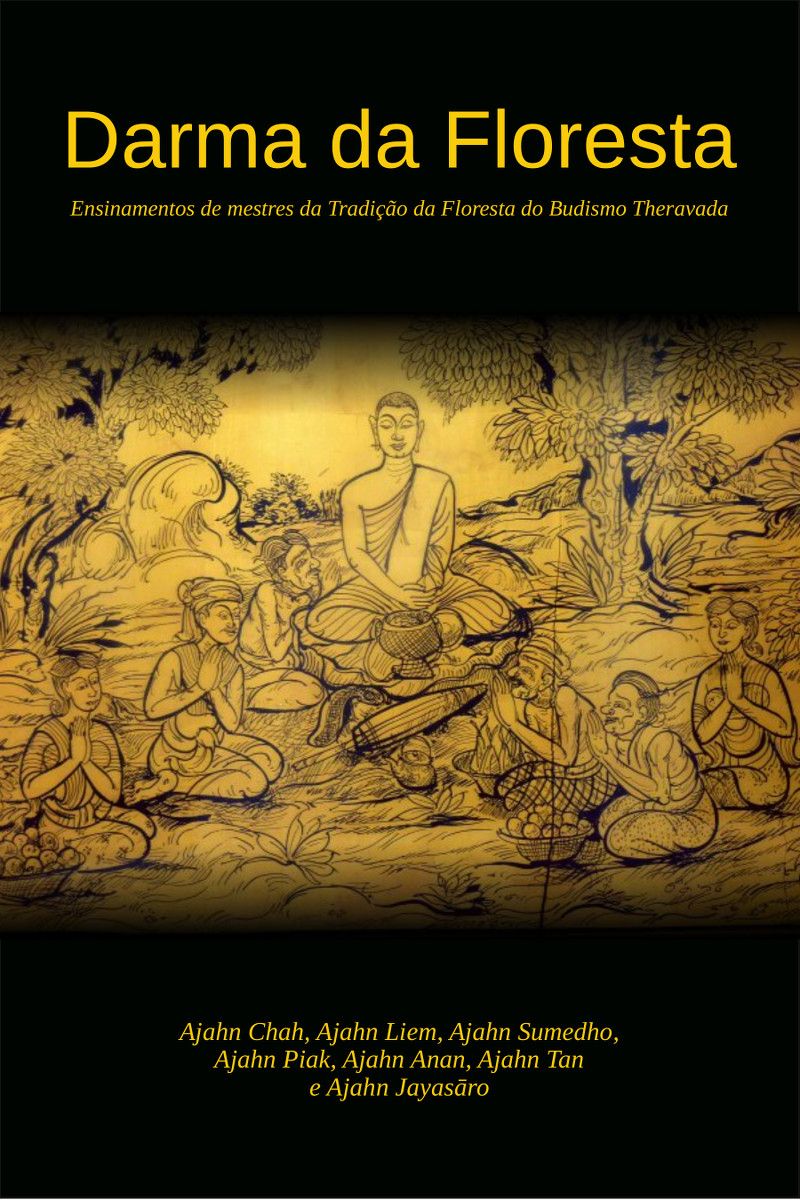
\includegraphics[height={\paperheight + 5pt}]{./webcover.jpg}%
}%
\fi

\frontmatter


\cleartorecto
\thispagestyle{empty}
\vspace*{5em}
\newlength\titleLength
\newlength\xheight

{\centering

\settowidth{\titleLength}{%
  {\Large\chapterTitleFont\scshape\MakeLowercase{\thetitle}}%
}

{\Large\chapterTitleFont\scshape\MakeLowercase{\thetitle}}\\[0.3\baselineskip]
\setlength{\xheight}{\heightof{X}}
\raisebox{0.5\xheight}{\color[gray]{0.4}\rule{\titleLength}{0.1pt}}\\[0.3\baselineskip]
{\itshape
Ensinamentos de mestres da tradição\\
da floresta do Budismo Theravada}

\vfill

Dhamma Desanās de Ajahn Chah, Ajahn Liem, Ajahn Sumedho, Ajahn Piak,
Ajahn Anan, Ajahn Tan e Ajahn Jayasāro

\vspace*{5em}

}




\cleartoverso

\thispagestyle{empty}

{\small\setlength{\parskip}{0.8em}\setlength{\parindent}{0em}%
{\raggedright%

\thetitle

Para distribuição gratuita\\
\emph{Sabbadānaṁ dhammadānaṁ jinati}\\
‘A oferta de Dhamma é superior a qualquer outra oferta.’

Publicado por Amaravati Publications\\
Amaravati Buddhist Monastery\\
Hertfordshire, Great Britain\\
abmpublications@amaravati.org\\
\href{http://amaravati.org}{www.amaravati.org}

Este livro encontra-se disponível para distribuição gratuita em\\
\href{http://forestsanghapublications.org/}{www.forestsanghapublications.org}

ISBN \theISBN

Copyright \copyright\ 2014 Amaravati Buddhist Monastery

Imagem de capa de autoria de Anandajoti Bhikkhu\\
Para mais informações visite \href{http://www.photodharma.net/}{www.photodharma.net}

\vfill

{%\footnotesize

Este trabalho encontra-se licenciado sob a
Atribuição NãoComercial\\ SemDerivações 2.0 Reino Unido: Inglaterra e País de Gales\\
\href{http://creativecommons.org/licenses/by-nc-nd/2.0/uk/deed.pt}{www.creativecommons.org/licenses/by-nc-nd/2.0/uk/deed.pt}

Veja página \pageref{copyright-details} para mais detalhes sobre direitos e restrições desta licença.

Produzido com o sistema tipográfico \LaTeX. Fonte utilizada: Gentium, distribuída por SIL International e Crimson Text, criada por Sebastian~Kosch.

%Produced with the \LaTeX\ typesetting system. Typeset in Gentium, distributed by SIL International, and Crimson Text, by Sebastian Kosch.

\theEditionInfo

}

}}



\cleartorecto
\tableofcontents*

% Preface by Ajahn Vajiro

\chapter{Prefácio}
\markright{Ajahn Vajiro}

Ajahn Mudito pediu-me que escrevesse um prefácio para esta coleção
de ensinamentos de \emph{bhikkus} da floresta da Tailândia. Eu
conheço Ajahn Mudito desde quando ele primeiro aspirou tomar o
treinamento como \emph{bhikkhu} no começo deste século – naquela
ocasião, apenas por e-mails. Desde que comecei a estar mais envolvido
em trazer da tradição da floresta do Budismo para os países de língua
portuguesa, nós tivemos mais contato.

Este trabalho é uma forma de transmitir os ensinamentos dos monges
da floresta da Tailândia. Ajahn Mudito está muito bem qualificado a
preparar esses ensinamentos para as pessoas do mundo que usam o
português como primeira língua. Ele vive a vida de um monge da floresta
na Tailândia e tem dedicado tempo e atenção em aprender destes Ajahns e
discípulos destes Ajahns. Muitos destes ensinamentos não estão
disponíveis em livros de nenhuma outra língua. Os ensinamentos são de
uma tradição oral, e Ajahn Mudito foi o primeiro a transcrevê-los. Eles
foram então utilizados para gerar legendas para vídeos dos Ajahns.
Aquele método foi bom e agora o formato de palavra escrita é um
acréscimo útil.

Estou muito contente que Ajahn Mudito tenha realizado este trabalho
e confio que será uma benção para muitas pessoas.

\bigskip

{\raggedleft
Ajahn Vajiro

Mosteiro Budista Sumedhārāma\\
Ericeira, Portugal
\par}



% Nota do tradutor

\chapter{Nota do tradutor}

Em Abril de 2012 comecei um trabalho de tradução, inicialmente
somente de textos de Ajahn Chah e seus discípulos e mais à frente
também de outros mestres tailandeses, discípulos diretos ou indiretos
de Tahn Ajahn Man Bhuridatto. O resultado pode ser encontrado no site
\href{http://www.dhammadafloresta.blogspot.com/}{www.dhammadafloresta.blogspot.com},
onde é possível ouvir a gravação original em áudio de todos os
ensinamentos contidos neste livro, assim como ver fotos dos mestres que
os proferiram. 

Com o tempo o número de palestras traduzidas no site foi aumentando
até que, seguindo sugestão de uma pessoa do site
www.ouvindoodhamma.com,, foi iniciado o trabalho de seleção de um
pequeno grupo de textos para publicação em forma de livro. Foram
selecionados oito textos de Ajahn Chah e um de cada um de seus
discípulos cujos ensinamentos constavam no site. A proposta do projeto
era transformar o conteúdo do site, que havia sido traduzido com ênfase
em ser o mais fiel possível às palavras dos mestres, num texto mais
amigável ao formato escrito e a um público iniciante. 

Neste livro, em vez do idioma páli, optamos por fazer uso máximo da
grafia portuguesa de palavras relacionadas ao ensinamento do Buda que
já foram incluídas oficialmente na nossa língua. Nominalmente: Buda
(\textit{Buddha}), Darma (\textit{Dhamma}), carma (\textit{kamma}),
nirvana (\textit{nibb\=ana}), parinirvana (\textit{parinibb\=ana}),
bodisatva (\textit{bodhisatta}) e páli (\textit{p\=ali)}. Todos os
demais termos ou foram traduzidos para o português, ou foram utilizados
em suas grafias originais, em páli. Apesar do esforço em traduzir o
máximo possível de palavras em páli para o português, uma grande
quantidade delas permaneceu em seu formato original. Em parte isso se
deveu à dificuldade em encontrar correlatos satisfatórios em português
e em parte pelo contexto em que os ensinamentos foram dados, como vai
ser explicado mais adiante.

Vale a pena mencionar que todos os ensinamentos de Ajahn Chah
publicados aqui são inéditos: jamais foram traduzidos ou publicados em
qualquer outra língua ocidental (a maioria deles nem mesmo em
tailandês) e o mesmo é verdade para a maior parte dos textos de seus
discípulos incluídos no livro. 

No que diz respeito à grafia de termos em tailandês, procurei manter
o padrão mais aceito para evitar confusões desnecessárias. Não existe
um só padrão para romanização de palavras tailandesas que realmente
funcione e por isso diferentes pessoas utilizam diferentes métodos. Por
exemplo, alguns escrevem “ajaan”, outros “ajahn”, outros “atchan” e
assim por diante. Não quero eu também inventar ainda mais um sistema de
romanização, mas uma vez que os sistemas mais populares foram
produzidos para um público anglófono, algumas distorções se apresentam
para nós que utilizamos a língua portuguesa e por isso eu abandonei a
grafia mais usual de algumas palavras: “Luang Por” (\thai{หลวงพ่อ}) foi escrito “Luang Pó”, “Ajahn Dtun” (\thai{อาจารย์ตั๋น})
foi escrito como “Ajahn Tan” e “Ajahn Mun” (\thai{อาจารย์มั่น})
como “Ajahn Man”. 

Um aspecto muito importante do conteúdo deste livro que precisa ser
mencionado é “contexto” – quem disse, para quem foi dito, quando, por
quê, etc. Em especial, quando falamos sobre mestres da tradição da
floresta tailandesa, discípulos de Ajahn Man, entender o contexto se
torna ainda mais importante, pois esses eram mestres que
verdadeiramente ensinavam de coração. A prática deles não ocorreu
dentro de um mundo fechado de livros, de conceitos e teorias: eles
usavam suas próprias vidas como combustível na busca do Darma e por
vezes levavam a prática às suas últimas consequências – muitos deles
chegaram à beira da morte (incluindo Ajahn Chah). 

E não é só essa característica que vem à tona quando ensinam; também
o fato de terem verdadeiramente experienciado em si mesmos níveis
elevados de realizações espirituais faz que seus ensinamentos tenham,
além de espontaneidade, um tom de autoridade que alguns podem achar
incômodo. Por essa razão, acho importante lembrar que os ensinamentos
contidos aqui, em sua maioria, ocorreram num ambiente onde havia um
real clima de amizade e confiança entre mestre e discípulos, onde o
mestre se sentia à vontade para falar abertamente sobre o assunto e em
utilizar uma linguagem mais sofisticada (pois sabia que a audiência
estava familiarizada com termos em páli). O resultado final é
um tanto paradoxal: ao mesmo tempo em que o ensinamento é extremamente
simples e direto ao assunto, também apresenta uma sofisticação de
linguagem que pode exigir do leitor um pouco de esforço em compreensão.
Para ajudar, muitas notas ao longo do texto – e também um glossário ao
final do livro – foram incluídas.

Outro aspecto relevante, principalmente quando o ensinamento é
destinado à comunidade monástica, é o nível de desenvolvimento
espiritual da audiência. Por exemplo: para uma plateia de iniciantes,
Ajahn Chah diz que as pessoas sofrem e não conhecem a si mesmas por não
possuirem \textit{sam\=adhi. }Em outra ocasião, onde os presentes
talvez fossem já bastante hábeis na prática de \textit{sam\=adhi, }ele
critica duramente e diz que \textit{sam\=adhi }“é o cúmulo da burrice”.
Isso deve ser entendido dentro do contexto: um grupo ainda não chegou
àquele nível, outro já chegou e agora precisa ser encorajado a
continuar seguindo adiante e não apenas contentar-se com o estágio
alcançado. A incompreensão desse fator já levou algumas pessoas (em
especial alguns professores leigos nos Estados Unidos) a defender que
Ajahn Chah tanto não ensinava como sequer elogiava a prática de
\textit{sam\=adhi} – nada poderia estar mais longe da verdade.

Por fim, devo mencionar que a compilação deste livro só foi possível
graças à ajuda de Angelo De Vita, com um trabalho importantíssimo de
revisão e consulta, e também Venerável Dhammiko, Gabriel Laera,
Jaqueline Szili, Jair Seixas e Carla Schiavetto, que ajudaram a revisar
e dar sugestões para a melhoria do texto final. Ainda assim, peço que
quaisquer omissões ou erros sejam de minha inteira responsabilidade.
Que o mérito dessa realização seja causa para que todos progridam no
Dhamma, em direção à paz e libertação – nibb\=ana. 

Anumodan\=a.

Mudito Bhikkhu

\textit{Wat Khao Sam Lan}

{\itshape
Nakhon Nayok, Tailândia}



\mainmatter

%\book{\thetitle}
% === Book ===

\cleartorecto
\thispagestyle{empty}
\vspace*{5em}

{\centering
\Large\chapterTitleFont\scshape\MakeLowercase{\thetitle}
\par}


\begin{quotepage}{0.63\linewidth}{Ajahn Chah}
Pensamos que felicidade não tem um lado ruim, mas não é assim.
Felicidade é a número um, ela mesma já é sofrimento. Quer seja
felicidade ou sofrimento, são como uma mesma cobra. Sofrimento é como a
cabeça da cobra, felicidade é o rabo da cobra. Vemos que essa cobra é
longa (…) e pensamos: ‘Eh, a boca é perigosa, o rabo não tem perigo,
(…) não vou chegar perto da boca senão vou tomar uma picada! É melhor
pegar pelo rabo porque a boca está daquele lado.’ Mas quando pegamos, o
rabo ainda é rabo de cobra, não é? A cobra se vira e vem morder, é
sofrimento do mesmo jeito, porque a cabeça da cobra está na cobra, o
rabo da cobra está na mesma cobra.
\end{quotepage}



% Conversa com um doutor

\chapter{Conversa com um doutor}

{\itshape
Conversa informal entre Ajahn Chah, um médico e sua esposa.}

\textit{(Dr.)} - Tanto quanto me lembro de ter lido uma vez, havia
uma pessoa de família pobre e esse garoto tinha inteligência, de forma
que os pais e os irmãos achavam que ele seria capaz de estudar e
conseguir se formar. Então os pais e os irmãos todos abriram mão de
estudar para conseguir economizar dinheiro para pagar os estudos deste
garoto. Todos passaram por muitas dificuldades. Esse garoto foi para a
universidade, mas também estudou o Darma e sentiu inspiração profunda.
Quando terminou seus estudos, aconteceu que… o pai, a mãe e todos os
demais tinham grande esperança de que, quando ele estivesse formado,
ele sustentaria a família. Seria capaz de trabalhar e ganhar dinheiro,
ajudando os irmãos mais novos ou ajudando a dividir o fardo do pai e da
mãe, ou seja, o pai e a mãe iam poder descansar um pouco para poder
ajudar os filhos menores, mais adiante. 

Mas aconteceu que esse garoto, quando acabou seus estudos, ficou
muito inspirado pelo Darma, a ponto de pedir licença do pai e da mãe
para não ir trabalhar, queria ordenar-se monge. O pai e a mãe choraram
e tentaram impedir, mas o filho disse ter muita fé no ensinamento do
Buda: “Não me impeçam!” No fim os pais tiveram que dar permissão para o
filho virar monge\footnote{Uma pessoa só pode virar monge caso
autorizado pelos pais.}, mas do meu ponto de vista, tanto quanto eu li
e ouvi dizer, sinto que eles provavelmente não o fizeram de muita boa
vontade. Essa história ficou presa na minha cabeça. 

\textit{(Ajahn Chah) }{}- Por quê? 

{}- Peço desculpas, Luang Pó, essa é apenas minha opinião, não sou
\textit{expert} em religião, mas penso que neste mundo tem que haver
duas partes: uma parte é a religião, outra parte são os donos de casa
normais, que necessitam exercer profissão, ganhar seu sustento. Por
exemplo: eu tenho família, tenho filho e esposa. Tendo eu
responsabilidade pela minha família, tenho que cumprir meu dever para
com eles. Estou vinculado a eles e tenho que cumprir meus deveres para
com a minha família, a sociedade, a nação. Agora, tanto quanto li aqui
neste lugar, talvez tenha sido escrito por outra pessoa, não sei… diz
que o objetivo é que todas as pessoas virem monges. Eu penso na minha
cabeça que neste momento sou dono de casa, sustento minha esposa e
filho com meu ofício, dou felicidade a algumas pessoas, dou ajuda a uma
parte da população e faço um pouco de doações ao templo, ou seja,
também ajudo a religião. Mas, se todos virarem monges, incluindo a mim
mesmo, os monges vão ter que arar a terra, vão ter que procurar ofício,
não terão tempo para praticar a regra monástica. Os monges não terão
oportunidade de aconselhar e guiar o povo, dar luz para que haja paz de
espírito, para que haja um caminho a seguir neste mundo. 

Por essa razão, na minha opinião, essa pessoa, se for virar monge
está bem, mas somente quando terminados seus deveres, ou seja, ajudar o
pai, a mãe e os irmãos. Ordenar-se agora, neste momento, se perguntar
para mim, se for para eu decidir dentro da minha ignorância, digo que é
uma maldade, muita maldade. Porque é machucar os pais e é uma maldade
para com os outros também, pois todos ajudaram essa pessoa, e aqui
surge o problema: essa minha opinião está certa ou errada?

{}- O doutor também tem razão. Vejamos assim, eu vou lhe fazer uma
pergunta: um quilo de ouro e um quilo de chumbo, se vierem dar ao
doutor, o que o senhor escolhe? 

{}- O ouro.

{}- Pois é, é assim mesmo. Quando uma opinião é firme dessa forma,
aquilo ganha um valor diferente, tal como ouro e chumbo, tem que
escolher o ouro. Eles trouxeram ambos, porque o doutor escolheu o ouro
e não o chumbo?

{}- Porque possui valor.

{}- Pois é, você enxerga que possui mais valor. Da mesma forma nesse
caso, ele enxerga mais valor do que isso a ponto de se decidir dessa
forma. É assim, é a mesma situação. Por isso não devemos pensar assim,
não há nada de errado em pensar, mas tem que refletir até ficar
correto.

Está com medo, hein? O doutor está com medo de que não haja quem
cuide dos pais, não haja quem construa o mundo? Se estiverem
contratando pessoas para tocar música o doutor não precisa se preocupar
pois eles só vão contratar pessoas que souberem tocar música. Se não
souber, como é o seu caso, eles não contratam. Não dá para pegar todas
as pessoas e fazê-las monges, mas proibir para que ninguém vire monge
também não dá. Essas coisas são assim mesmo, não devemos pensar: “que
todos virem monges!”, não dá. “Que ninguém vire monge!”, dá? Não dá,
não é possível, não dá para forçar desse jeito. Aqui temos que enxergar
o que há: quem tiver sabedoria, a que nível, que aja de acordo.

Eu também já passei por isso. Fui dizer que matar animais é demérito
e uma pessoa respondeu: “Luang Pó consegue comer pimenta pura todo
dia?” 

Respondi: “Não, pois não há quem traga pimenta para eu comer todo
dia, tem alguém? Vá buscar, prepare pimenta para eu comer todo dia,
pode ser?” Não concordou. Quem vai ter tempo de preparar pimenta para
monge comer todo dia, sem falta? Esse tipo de conversa é só da boca
para fora, mas neste mundo é assim mesmo. Forçar todas as pessoas a
serem boas ou ruins é impossível. Quem tem sabedoria neste mundo,
escolhe. “Vejam este mundo enfeitado como uma carruagem real, onde
tolos afundam, mas nos sábios não há apego.”\footnote{Verso do
Dhammapada (Lokavagga – 171)} Essa é a garantia que o Buda nos dá. 

Então, nossa intenção em virar monge não é ver nossos pais
perecerem, nossos filhos perecerem, nossa família perecer ou algo do
tipo. Pensamos: “Puxa, minha família está atolada demais na lama, na
sujeira. Se nem eu conseguir sair, estaremos todos presos, assim será
uma perda total…” Então nos esforçamos para sair, por nossa família,
para que nossa família melhore. Mas algumas pessoas chegam a pensar que
não há proveito, que é maldade, como o doutor. Se olharmos por esse
ângulo, é assim. Por isso perguntei: um quilo de chumbo e um quilo de
ouro, se formos dividir, qual você escolhe? 

Isso é igual. Quando ele decidiu virar monge pelo resto da vida
daquele jeito, ele viu que isso tinha muito mais valor, viu o mundo
inteiro como se fosse chumbo, sem valor, portanto não o deseja. Igual
ao doutor que deseja um quilo de ouro mas não quer um quilo de chumbo,
por quê? Porque possui pouco valor, não tem valor, portanto decidiu
pelo ouro dessa forma. Se soubermos refletir, não é o caso que nos
ordenamos para destruir nossos filhos, destruir nossa esposa, nossa
família ou algo do tipo, não é assim. Não é assim.

Isso é muito difícil pessoas conseguirem fazer: alcançar o máximo de
sabedoria até chegar ao ponto que o doutor viu, onde tudo vira do
avesso. É como ser capaz de fazer a palma da mão virar as costas da
mão. Se a pessoa só consegue enxergar da forma que o doutor enxerga,
ainda não será capaz. Ele age daquela forma com boa intenção e está
correto, age por enxergar de verdade os princípios do Darma. 

Se não é assim, então nosso Buda… é só maldade! O Buda é só maldade.
“Não importa quanto sofrimento minha família passe, mas vou ajudar
essas pessoas, ensinar essas pessoas a vir para a luz. Elas já ficaram
na escuridão tempo demais.” – pensando desse jeito ele decidiu
ordenar-se. Como o filho do coronel Pramôt\footnote{Este rapaz
continuou na vida monástica e eventualmente tornou-se um grande mestre.
As pessoas hoje o conhecem pelo nome Ajahn Piak.}, que terminou os
estudos no exterior e veio ordenar-se aqui comigo. Ordenou-se e decidiu
não voltar à vida laica. Inicialmente o pai viu e pensou: “Oh! Quanto
sofrimento!”, mas hoje em dia ele vai ao monastério com frequência,
ouve o Darma com frequência. Hoje em dia não quer mais ficar aqui na
cidade, quer fugir para Wat Pah Pong, não quer ficar aqui. Há uma
mudança quando enxergamos aquilo que antes não enxergávamos e vemos que
não há benefício algum. Existe benefício porque possuímos sabedoria, se
não temos sabedoria não enxergamos benefício naquilo. 

Mas não pense errado: “Todo mundo virou monge, quem vai morar neste
mundo?” Oh! Ainda mais gente, Sr. Doutor! Não é assim! Não pense que o
mundo vai desvanecer – vai ficar ainda mais firme! Não pense que o
mundo vai ficar ralo – vai ficar ainda mais espesso. Quando o senhor
virar monge o senhor vai explicar sobre a maldade para que as pessoas
entendam, fiquem em paz e tenham felicidade – se não muita, então
pouca. Ajudamos. Ajudamos a pegar a bondade e o que há de bom e ensinar
razão: “Não se agridam, afinal todos temos que ganhar a vida, buscar
nosso sustento. Não agridamos uns aos outros!”, todos os pontos de
vista como esse. Se pensarmos: “Eh, se todo mundo virar monge vai ser
uma desgraça”, ninguém vai poder virar monge. 

Veja os dedos da sua mão: Não puxe os dedos para que eles tenham
todos o mesmo tamanho! Esse dedo é assim, aquele é de outro jeito.
Mesmo não sendo todos do mesmo tamanho, ainda são úteis? Têm a
utilidade deles. Pegue esse pequenino aqui, é útil? Se não for do mesmo
tamanho que os demais, corta fora? Do jeito que é ainda serve para
cutucar o nariz! É muito útil. Não podemos pensar desse jeito pois é
uma união. O mundo não pode ser do jeito que o senhor diz, ou então não
é mundo. Desse jeito o mundo não é mundo. Não seria mundo. Mas é
justamente por ser mundo, que é assim. 

Bem onde está certo ensinamos, mas as pessoas não enxergam. Falam
que sim, mas não enxergam. Bem aqui está errado, ensinamos: “bem aqui
está errado”, mas não enxergam. Mas, para alguns, é só verem que ali
está errado e logo entendem, veem que ali está certo e logo entendem.
Algumas pessoas conseguem ver certo e errado. Não fique com medo que o
mundo vá desvanecer. Não pense que não haverá quem construa o mundo no
futuro.

{}- Eu entendo, Luang Pó. Eu tenho um amigo que é monge, estávamos
conversando sobre esse assunto de fazer doações ao templo. Eu disse a
ele que não faço muitas doações, vez por outra apenas. Estávamos
conversando sobre isso e escutei um fundamento correto. Conversávamos
sobre as pessoas que fazem doações. Tal qual tenho observado já faz
algum tempo, algumas pessoas são pobres a ponto de quase não ter o que
comer, os filhos não têm o que comer, mas tendo dinheiro, os pais o
guardam para comprar durian\footnote{Fruta típica da região sudeste da
ásia, na época era considerada um artigo de luxo.} para dar aos monges.

Eu perguntei se isso estava correto. Meu amigo disse que está
errado, doações têm que ser feitas sem ser um fardo. Não deve ser:
“Puxa, nossos filhos ou nós mesmos queremos comer, temos para comer,
mas não vamos comer! Vamos dar para os monges comerem! Assim vamos
ganhar mérito.” Meu amigo monge disse que isso está errado. Doações
devemos fazer na medida em que é possível e não sendo um fardo para os
demais. É como nessa história que ficou presa na minha cabeça, do rapaz
que se formou e virou monge, eu penso que essa história de fazer mérito
deve fazer nascer felicidade no nosso coração e no das demais pessoas.
Não é como: “OK, vou roubar a carteira dessa pessoa para ir fazer
mérito.” Essa pessoa ia usar o dinheiro para cuidar do filho que está
para morrer no hospital e eu vou lá e roubo, aquilo traz sofrimento
para outras pessoas. Da mesma forma eu insisto, é por isso que não
consigo aceitar que essa pessoa que se formou e virou monge ganhou
mérito. Eu entendi o que o senhor me ensinou agora pouco, mas eu
insisto nisso: se for fazer mérito, não é correto que acabe em maldade.
Quer dizer, um grupo de pessoas ter que sofrer. Caso alguém faça
mérito, tem que gerar felicidade no coração de todos os envolvidos. 

Por essa razão, esse monge que se ordenou, como já disse, mesmo que
ele vá ensinar e propagar o Darma ou o que seja… Mas se for perguntar
para mim, eu digo que esse monge ainda é moleque em primeiro lugar –
ainda é moleque. Já há o senhor Luang Pó aqui, o senhor Ajahn ali, e
quantos mais que já estão cumprindo a tarefa de propagar o Darma. Mas
esse aí vai querer fazer como se fosse o Buda que abandonou o Rahula, a
rainha, e foi se ordenar\footnote{Siddattha Gotama, que eventualmente
tornou-se o Buda, abandonou sua esposa e filho recém-nascido para viver
uma vida ascética e buscar o caminho para a iluminação.}? Aquilo é o
Buda, o líder, o nosso mestre, o pioneiro, os outros ainda não eram
capazes de enxergar, ainda possuíam muitas impurezas, ainda não eram
capazes de enxergar o caminho para que haja felicidade para a maioria
das pessoas. 

Eu não elogio a ordenação desse monge, no momento atual já há o
Luang Pó aqui, aquele Ajahn ali, aquele outro lá. Vários que proclamam
o Darma de forma que possamos estar aqui hoje. Portanto essa pessoa não
é importante tal qual o Luang Pó, ou a ponto de se fazer como o Buda.
Isso me faz censurá-lo. Eu censuro fazer mérito sem refletir sobre o
momento apropriado. Se esperássemos dois, três, cinco anos e tivéssemos
resolução firme, não desistiríamos. Teríamos firmeza em praticar o
Darma até que chegasse o momento apropriado. Quando não gerasse
sofrimento para os demais, não gerasse dificuldades para os demais,
quando surgisse satisfação em todos com nossa fé, então sim, seria o
momento apropriado para ordenar-se. Eu censuro muito ele não ter
escolhido o momento correto, é o que eu considero uma maldade. É por
essa razão que eu vim aqui, com todo respeito, discutir com o senhor.
Eu digo que o momento não era apropriado.

{}- Me diga, onde você vai encontrar alguém que saiba prever o
futuro desse jeito?

{}- Essa pessoa, se aguentasse firme mais sete anos e então se
ordenasse – dessa maneira seria uma boa pessoa. Mas supondo que
passados sete anos desistisse, fosse ter esposa, beber cachaça – nesse
caso é uma pessoa ruim, não serve.

{}- Onde você vai encontrar isso? Todo mundo quer ser assim. Se for
“sete anos para se ordenar”, a morte vai esperar? Ele enxergou assim
antes de ir. Morte: “sete anos e então morre”, há algum acordo? As
pessoas nascem, mas na hora de morrer: “sete anos para virar monge!”
Ninguém sabe. Tem algum acordo? Quando uma pessoa vê dessa forma, o que
ela pode fazer? Ela não tem certeza sobre sua própria vida. Eu digo
que, de todas as pessoas, não há quem tenha um acordo do tipo: “setenta
anos, oitenta anos e então morre”, não existe, não tem como saber. Ele
olha e não enxerga sua própria morte, ele não confia em sua própria
morte. Se ele enxerga dessa forma ele vira monge com certeza. Por que
não? Se aquela pessoa enxerga dessa forma! Não é que nem nós aqui. Nós
aqui temos que obrigar a ser “seis, sete anos” para que chegue a hora.
\textit{Akaliko} – morte tem dia e hora? Se aquela pessoa vê dessa
forma, o que é que você quer que ela faça? 

{}- Eu digo que essa pessoa é egoísta. 

{}- Hum?

{}- Essa pessoa é egoísta.

{}- É o quê?

{}- Egoísta. Por quê? Ela toma a felicidade, que é o deleite na
religião, sozinha. 

{}- Se é assim, tenho que dizer o seguinte: o doutor aprendeu
medicina, portanto é egoísta.

{}- Correto, correto.

{}- Pois, é! Sabe por quê? Se ainda existe um ego, ainda há egoísmo.
Mas pessoas que agem desta forma e não são egoístas também existem.
Como o Buda – não foi egoísta, ele destruiu seu próprio ego. Essa
palavra “ego”, “ego”, é apenas uma convenção. Uma pessoa que consegue
atingir aquele ponto não tem mais ego. Nós somos egoístas, então
pensamos que os outros devem ser iguais a nós, pensamos que ele é
egoísta, mas o ego dele já não existe. Há terra, fogo, água e ar, não
há ego. Essa expressão “ser egoísta” pressupõe que terra, água, fogo e
ar são nossa pessoa, são um ser, uma pessoa desse jeito. Esse tipo de
expressão e esse tipo de entendimento estão incorretos e vão juntos
infinitamente. 

O ponto mais alto do ensinamento do Buda é a ausência de pessoa – há
terra, água, fogo, ar, agrupados em uma pilha, só isso. Animal ou
pessoa não existem. Se aquela pessoa atingir esse ponto, como é
possível ele ser egoísta? Pois já não há ego. O que nos faz ser egoísta
é ter um ego dessa forma. Se formos falar sobre não ter ego, ninguém
entende. Conversar sobre coisas mundanas e coisas transcendentes não é
igual. Por exemplo, se eu descrever para o doutor a seguinte situação:
se dissermos “andar para frente” – conhecemos, “andar para trás” –
conhecemos, “ficar parado” – conhecemos. Se vier mais uma frase que
diga: “nem andar para frente, nem andar para trás, nem ficar parado”,
como é que fica? A expressão “andar para frente”, conhecemos. “Andar
para trás”, ouvimos e entendemos. “Ficar parado”, entendemos. Mas vem a
segunda frase: “nem andar para frente, nem andar para trás, nem ficar
parado”, como é que fica? Essa pessoa chegou a um certo ponto, já
aquela chegou a um ponto mais adiante, é assim.

Eu insisto: conversa mundana e conversa sobre o Darma mais elevado –
estendemos a mão, mas não alcançamos. Andar, caminhar – conhecemos.
Andar para trás – conhecemos. Ficar parado – conhecemos. Não andar para
frente, não andar para trás, não ficar parado – não conhecemos, ouvimos
e fica por isso mesmo. Bem aí, aí é que as pessoas não entendem nada a
ponto de haver tantos problemas e confusão demais desse jeito. Mas essa
frase é a forma de expressão daqueles que estão além deste mundo, é a
forma de expressão dos \textit{aryias}.
Crescemos a esse ponto, antes éramos crianças, não
é? Éramos crianças pequeninas, e agora crescemos a esse ponto. Sente
saudades de ser criança? Lamenta não ser criança? Por que foi possível
crescer a esse ponto? Porque é assim: entra comida por aqui, não é
assunto nosso, é assunto do mundo. 

Falamos, mas não acertamos o alvo… Mas todo mundo tem, todo mundo
neste mundo diz ter razão… É verdade, mas quando todo mundo vai
inventando razões, as razões acabam diferentes umas das outras. Gente
burra tem razão, gente esperta tem razão. Gente esperta tem a razão
deles, gente burra tem a razão deles. Significa que essa história de
razão não tem fim. Quando o Buda diz: “Eu ajo além dos motivos, acima
das razões. Além de nascimento, acima da morte. Além da felicidade,
acima do sofrimento”, e aí, como é que fica? É uma história
completamente diferente, completamente diferente. 

Por exemplo, o doutor foi criança, alguma vez brincou com balão
inflável? Via o balão e ficava feliz e alegre por causa do balão:
“oba!, oba!”. Agora cresceu a esse ponto, não é? É diferente de quando
era criança, não pensa mais em brincar com esse tipo de coisa. Por que
não quer brincar? Pois não há utilidade! Já cresceu, vê? Não há
utilidade. Quando éramos crianças, naquela época, víamos o balão como
algo muito valioso. Brincava e se divertia, “oba!, oba!” – sozinho. Não
sabia de nada. Mas quando o balão explodia “pôp!” – chorava… Por que é
assim? Brincar com essas coisas é o que se chama “nossa mente estar
fixa”. 

Então nossa idade se desenvolve, mudamos com o tempo e crescemos a
esse ponto. O doutor ainda vai brincar com balão, como as crianças?
Pois é assim. Como vamos resolver esse problema, quando é o caso que
aquele rapaz pensa dessa forma? O doutor tem que dizer: “Eu não quero
brincar pois não há utilidade.” E as crianças? Isso contradiz a opinião
das crianças. O doutor diz: “Não tem utilidade.”, mas as crianças
discordam do doutor: “É útil sim!” E aí, quem vence? Quem está certo,
quem está errado? As crianças têm as razões delas, os adultos têm as
razões deles, são mundos diferentes. Tem que ser assim. 

Ótimo! As perguntas hoje estão muito boas, quero que faça muitas
perguntas e assim se esclarece. São duas coisas completamente
diferentes, completamente diferentes…

{}- Estou conseguindo enxergar.

{}- Pois é. 

{}- Eu tenho uma opinião, é uma opinião que inventei sozinho, tenho
que admitir. Minha esposa aqui, Pao, cerca de dez anos atrás… Nossa!
Vivia se benzendo\footnote{É comum as pessoas na Tailândia pedirem que
os monges abençoem água para que elas borrifem sobre si para espantar
más energias ou trazer boa sorte.}! Eu perguntava: “Está possuída por
um espírito maligno? Foi fazer algo ruim ou o quê?” Seja lá o que
fosse, tinha que se benzer. Ela chamava para que eu fosse junto mas eu
dizia: “Não fiz nenhum mal, no que diz respeito à minha profissão,
ajudo as demais pessoas. Isso é um tipo de bondade e, em geral, quando
trabalho, trabalho com intenção de fazer direito. Caso cometa um erro,
é sem ter tido intenção, é por não ter tido conhecimento suficiente ou
por ter me equivocado, sem ter intenção de prejudicar ninguém. Eu digo
que não faço maldade.”

Não estou possuído por um espírito maligno, não fiz maldade, então
não me benzo. Pelo contrário, penso que a religião, qualquer que seja,
ensina a ter amor uns pelos outros, a praticar o bem da forma que o
mundo inteiro respeita e a tentar ser uma pessoa pura. Se formos de
acordo com a minha opinião, caso a pessoa chegue a um certo nível,
tendo encerrado seus deveres mundanos, suas responsabilidades, caso
queira ir procurar paz verdadeira – vira monge de vez, vai morar num
local pacífico. Mas só quando não tenha mais preocupações como: “Eh!
Meu filho não vai ter recursos para estudar, como é que fica?” Eu vou
ter que aprender a ser médium, a fazer água benta, a fazer poção
mágica\footnote{Muitos monges na Tailândia ficam ricos vendendo esse
tipo de “serviço”, embora o Buda tenha proibido aos monges possuir
dinheiro e muito menos realizar esse tipo de atividade, que ele
considerava serem “artes de animais”. }, isso não é correto. É por isso
que tenho a opinião de que fazer mérito, e então obter mérito ou não,
depende do coração – se nosso coração for puro, se agirmos sem ter más
intenções, sem maus pensamentos, mesmo que erremos, não acertemos o
alvo, mas tenhamos sensibilidade e procuremos corrigir, essa é uma ação
que penso ser pura o suficiente. Por isso esse tipo de “exibição”, por
exemplo, virar monge – chega a idade costumeira e “pap!”, ordena-se
monge porque mandaram. Quer dizer, ordenou-se por causa das
tradições\footnote{Antigamente era comum na Tailândia que todos os
rapazes se ordenassem monge ao completar vinte anos, por um período
curto de tempo.}, mas no coração talvez não haja paz suficiente ou
pureza suficiente, ou há preocupações e deveres por cumprir. 

Tanto quanto me lembre, temos que receber autorização para
ordenar-se monge e essa permissão deveria ser dada com sinceridade, não
por ter implorado, ter forçado o pai e a mãe dizendo: “Não quero nem
saber, vou virar monge, se me proibirem vou fazer algo ruim…” Isso é
obrigar, e eu digo que é fazer maldade. Por isso digo que, se for
fazer, se for ordenar-se para gerar bondade, depende do coração. Todas
as formas de fazer mérito… como no meu caso: eu tenho preguiça de doar
\textit{pindap\=ata}, mas minha esposa doa todos os dias pela manhã. Eu
tenho preguiça de tirar os sapatos\footnote{Quando os monges saem de
manhã pelas ruas recolhendo comida para sua refeição, as pessoas
costumam tirar os sapatos em gesto de humildade na hora de doar os
alimentos.}, mas não penso nada de mal, não penso de maneira ofensiva,
de maneira que tenho a opinião de que mesmo que alguém faça mérito até
morrer, na minha cabeça eu penso que mesmo que faça mérito até cair
morto, se no coração houver apenas ganância, confusão, arrogância ou se
fizer que os demais sofram, eu digo é melhor parar de fazer mérito
imediatamente. Vá aprender a fazer o coração ficar bom, a fazer as
outras pessoas felizes. Estou errado?

{}- Sobre isso aí, escute primeiro, OK? Existem duas coisas: número
um – a dona de casa se benzendo não deve estar certo.

{}- Mas agora ela já parou.

{}- O que será que aconteceu?

\textit{(esposa do Dr.)} - Eu sinto que me faz feliz, quando doo
\textit{pindap\=ata} fico feliz.

\textit{(Ajahn Chah)} - Pode deixar, eu vou explicar, vou resolver
essa questão. Por que age dessa maneira? Imagine uma galinha que temos
em casa: ela cacareja e corre para perto de nós, damos um par de calças
para ela – ela não aceita. Damos uma camisa – ela não aceita. O que
vamos dar para ela? 

\textit{(Doutor)} - Milho.

{}- Damos milho. Isso é útil para a galinha, não é? Só isso e já é
útil, ela quer aquilo. Camisa é bom só para pessoas, calça é para
pessoas, ela ainda não chegou ao nível humano, o que ela quer é milho.
Ela vem nos procurar, mas nós damos uma camisa e a galinha não aceita,
é melhor dar milho, não é? Desse ponto em diante ela vai melhorando,
melhorando, até virar gente. Quando for gente, se dermos milho para
comer ela não come. No começo é assim, e o doutor mencionou um segundo
item, o que era?

Ah! O senhor disse: “Eu não quero fazer mérito ou, se fizer, pego
minha mente e a transformo em mérito logo de vez.” Mas se o doutor for
uma pessoa esforçada, sendo uma pessoa esforçada, ia aguentar não
trabalhar? Ia aguentar não varrer a casa, ia aguentar não lavar os
pratos ou fazer algo de útil? Se for esforçado, não estou falando de
gente preguiçosa. 

{}- Trabalharia o tempo todo.

{}- Pois é, tem que ser assim. Para as pessoas que têm fé, fazer
doações é bom, mas o que o doutor disse sobre passar do limite também
está correto. Tem que saber moderar, tem que saber o suficiente,
conhecer moderação. Fazer demais sem considerar razão, não dá. Mas a
pessoa que tem fé profunda tem que doar \textit{pindap\=ata }ou fazer
\textit{p\=uja }e assim por diante, aquela pessoa está cheia de fé. Não
é para fazer como os tolos, mas para fazer como os sábios. 

Então podemos comparar com o doutor aqui, que é uma pessoa esforçada
ao máximo, não é preguiçoso naquilo que gosta. Vê a casa bagunçada,
consegue não varrer? Vê os pratos sujos, consegue não lavar? Vê o
cachorro vindo fazer cocô bem ali, toca ele para fora ou o quê? O
doutor tem que ser incapaz de parar de trabalhar, uma vez que é uma
pessoa esforçada. Aqui é a mesma coisa, tem que pensar dessa forma. Por
que age dessa maneira? Isso se manifesta vindo do coração de uma pessoa
esforçada, tem que ser assim. Se for o caso que ela ofereça
\textit{pindap\=ata} à toa, sem noção de nada, eu concordo contigo, mas
se ela faz tendo motivo como o doutor – por que limpa titica de
galinha, por que limpa cocô de porco, por que limpa cocô do cachorro,
por quê? Porque o doutor é detalhista da maneira correta, é uma pessoa
esforçada, não pode ver algo desarrumado, tem que limpar e arrumar. É
ali que se manifesta, não é só passar a tarefa adiante. Essa é a razão.


Aquilo, deixa para ela. Que ela vá atrás de água benta, deixa para
ela. Ela está no nível de galinha, que fazer? O nível é de galinha, mas
o doutor vai oferecer camisa – ela é galinha, não aceita. Que fazer?
Tem milho, então joga para ela comer, é melhor assim, para que ela
fique feliz. Tem que separar em níveis desta forma para poder chamar-se
“pessoa de entendimento”. Então o doutor vá contemplar tudo isso.

Ótimo! Hoje foi muito bom, o doutor já veio duas vezes mas ainda não
havia feito nenhuma pergunta. Ótimo, bote todas as perguntas para fora,
para acabar de vez desse jeito, bote para fora até acabar…


% Budismo estilo Theravada

\chapterAuthor{Ajahn Chah}
\chapterNote{Palestra dada por Ajahn Chah a praticantes leigos na Inglaterra.}
\chapter{Budismo estilo Theravada}
\tocChapterNote{Palestra dada por Ajahn Chah a praticantes leigos na Inglaterra.}
\markright{\theChapterAuthor}

Hoje vim aqui porque meus discípulos, como por exemplo o Sr. Suchin,
convidaram para que viesse me encontrar com as pessoas daqui. Pode-se
dizer que é muita sorte termos nos encontrado aqui. Alguns talvez não
saibam o que é isso que está sentado bem em frente deles. Somos monges
theravada que vêm da Tailândia, fizemos o esforço de vir até aqui hoje.
Viemos nos encontrar aqui hoje para sabermos como é o Budismo
Theravada. Na Tailândia há um local chamado Wat Nong Pah Pong onde há
muitos ocidentais indo estudar a prática da meditação budista. 

O Budismo Theravada que trouxemos aqui é um ensinamento que é sempre
atual, nunca envelheceu, nunca foi danificado e sempre acompanhou os
tempos e as pessoas também. Sempre ensinou todos nós a termos harmonia
e integração como se fôssemos um, com harmonia firme. Por exemplo,
ensina a todos nós de uma mesma maneira: aquilo que é ruim, que
perturba, não é pacífico, é confuso – somos ensinados a tentar
abandonar todas essas coisas. 

Depois disso nos ensina a ter sabedoria, a conhecer o que é errado e
causa perturbação para os indivíduos e para a sociedade como um todo
também. Esses ensinamentos, reunidos, são os pilares do \emph{Buddha
Sāsanā} e se chamam \emph{Sīla, Samādhi, Paññā}.

Em seguida somos ensinados a pacificar nossa mente. Esta nossa mente
aqui, mesmo tendo uma casa enorme para que viva bem, ainda não tem
bem-estar, pois ainda está fervendo por causa da confusão, por causa do
modo errado de enxergar as coisas. Estou falando sobre a mente de todos
nós aqui.

Agora vamos tentar concentrar nossas mentes, unificar a mente com um
objeto, o que se chama \emph{samādhi}. Portanto, prestem atenção no
que vou dizer. Fazer nossa mente ter força é diferente de fazer nosso
corpo ter força. Para que nosso corpo tenha força temos que correr, nos
movimentar, de manhã e à noite. Essa movimentação faz nosso corpo ficar
forte. Já a mente, devemos fazer que ela pare e permaneça quieta, fazer
que se pacifique. Isso trará energia, a mente terá força, isso se chama
\emph{samādhi}. Fazer a mente entrar em \emph{samādhi} não
acontece instantaneamente, porque desde que nascemos nunca treinamos
nossa mente a ficar quieta, nunca treinamos nossa mente a ficar em paz.
Nunca fizemos, então não vai ser logo hoje que vamos conseguir
pacificar nossa mente. Por isso temos que ter determinação em praticar,
quer haja paz ou não. Algumas pessoas, que nunca praticaram, têm medo.
Têm medo que fazer a mente se pacificar vá fazê-los ter problemas
mentais. Têm medo de ficar loucos e todo tipo de coisa. Por que isso?
Porque nunca praticaram, então ficam com medo. Não há nada disso. 

Sentem-se da forma que acharem melhor, mas sentem-se em paz. Tenham
uma postura pacífica e confortável. Todos fechem os olhos e foquem a
atenção na respiração, experimentem. Experimentem focar a atenção na
respiração, façam agora. Façam. Quem quiser sentar na cadeira – sente.
Quem quiser sentar no chão – sente. Pratique agora mesmo, quando
inspirar ou expirar esteja ciente. Não force a respiração a ser mais
rápida ou mais devagar. Não force a respiração a ser mais forte ou mais
fraca. Deixe que ela seja natural e tenha apenas ciência da respiração
entrando e saindo à vontade. Vocês veem a respiração? Estão cientes
dela? Como ela é? Como é “aquele que está ciente?” Vocês enxergam nas
suas mentes? Onde está “aquele que está ciente?” Onde está a
respiração? Como é a respiração? Foquem dessa forma, estejam cientes.
Usem a ciência dessa sensação para acompanhar a inspiração e a
expiração, acompanhem a respiração entrando e saindo à vontade. O seu
dever neste momento não é grande, basta estar ciente da respiração
entrando e saindo. Não precisa pensar: “O que vai acontecer se eu focar
a atenção na respiração? Vou saber alguma coisa? Vou ver alguma coisa?”
Não é dever de vocês pensarem nisso. O dever de vocês é estarem cientes
da respiração entrando e saindo e é só isso.

Normalmente não fazem isso. Há muitos anos, muito tempo, que vêm
negligenciando a respiração, não estão cientes de que o ar entra e sai.
Hoje que possuem esta oportunidade, observem como ele entra, como ele
sai, observem bem. A respiração possui muito valor, é a comida mais
importante dentre todas. Se não comermos esse tipo de comida por duas
horas é um problema sério; já comida como o arroz, mesmo se não
comermos por um ou dois dias, ainda conseguimos sobreviver. A comida da
respiração, se faltar por cinco ou dois minutos, não aguentamos.
Portanto, a respiração tem valor. Hoje todos vocês observem em detalhe
a respiração. Observem a respiração, não deixem a mente escapar para
cima, para baixo, para a esquerda ou para a direita, nem para frente ou
para trás. Que a mente esteja ciente somente da respiração na ponta do
nariz, só isso. Não pense que ficará com problemas mentais, que ficará
louco. Quanto melhor praticar, mais são vai ficar. Vai ficar são, vai
se curar de seus problemas mentais. Não pense que será de outra forma.
Pratiquem.

\clearpage

{\centering\itshape
-- intervalo para prática de meditação --
\par}

\ldots{} Nós não nos conhecíamos previamente, acabamos de nos conhecer
aqui hoje. Eu que estou ensinando, caso diga algo errado ou
inapropriado, me perdoem, me desculpem. Todos nós, naquilo que ainda
não conhecemos, somos ignorantes. Daquilo que ainda não estudamos,
somos ignorantes. Entendam isso. A mente da maioria das pessoas não se
aquieta. Por exemplo, hoje viemos nos sentar em paz desse jeito, as
pessoas que se acham espertas devem perceber: “Puxa, não tem paz
nenhuma, que barulho é esse vindo me perturbar? Barulho das crianças,
barulho dos barcos, vindo perturbar, todo tipo de barulho\ldots{} não há paz.”
A pessoa acha que está pesando de forma correta por causa da sua
esperteza, mas ela não enxerga a burrice naquilo. É o barulho que vem
nos incomodar ou nós é que vamos incomodar o barulho? Isso nunca
pensam. Na verdade somos nós que vamos perturbar o barulho, não é o
barulho que vem nos perturbar. É assim ou não é? Nós vamos perturbá-lo
ou ele vem nos perturbar? Olhem. Pois é, somos burros desse jeito. As
pessoas espertas são burras desse jeito. E ainda assim não admitem. Não
sabemos dessas coisas, pois só olhamos o lado de fora, não olhamos o
lado de dentro. Pensamos que somos espertos mas, na verdade, nós é que
vamos perturbar. Mas pensamos que é ele que vem nos incomodar. Isso é
causa para que não tenhamos bem-estar, é causa para nossa mente não ter
paz nem bem-estar, ficar confusa, pois não conhecemos a nós mesmos.

Como o mundo hoje em dia, todos os países, eles são do jeito que
são, eles não têm nada de mais. Somos nós que pensamos: “Esse é bom,
aquele não é,” gostamos desse, não gostamos daquele e só encontramos
confusão. Na verdade o mundo é do jeito que é. Não conhecemos sobre nós
mesmos, pois somos burros. Vários dos meus discípulos vão estudar nas
universidades do ocidente. Estou falando sobre meus discípulos: estudam
e ficam ainda mais burros, sofrem ainda mais, brigam ainda mais, não se
entendem. Disputam entre si, só brigam, não trabalham. Isso é porque
não conhecem a si mesmos. Hoje eu vim falar sobre a ciência do Buda,
hoje vamos estudar ciência do Buda. Hoje em dia tem muitas ciências, é
de perder a conta as ciências que estudamos. Mas essas ciências não se
complementam. Todas as ciências têm que incluir a ciência do Buda. Se
não incluir a ciência do Buda, não serve. Ainda não se harmonizam,
ainda disputam entre si, ainda têm inveja, ainda guardam rancor, ainda
geram confusão o tempo todo.

Hoje eu aproveitei essa ocasião para dizer isso, trouxe esse
presente. Se você é assim, corrija a si mesmo! Na nossa mente há algo
que não é bom? Aos poucos expulse para fora. Não acumule, aos poucos
expulse para fora. Aquilo que não for bom, que oprima a si mesmo,
oprima aos demais, aquilo na mente que não é bom, apenas expulse para
fora, não deixe acumular até ficar pesado. Como ponto inicial da
ciência do Buda, somos ensinados sobre \emph{Sīla}. 

Número um: não oprimir aos demais seres, pequenos ou grandes,
humanos ou animais. Isso é ciência do Buda para não sofrermos.

O segundo aspecto é que não guerreemos pelas coisas, deixem estar.
Não fiquem disputando os objetos, deixem estar. Isso é ciência do Buda.

O terceiro, se formos leigos: é normal termos família, não traia sua
família. Se trair sua família será mais um assunto para gerar
sofrimento.

O quarto é ser honesto: não minta, tenham sinceridade entre si,
todos vocês. Esse é mais um ponto da ciência do Buda.

O número cinco é não beber coisas que embriagam. Já estamos
embriagados o suficiente na nossa mente com todo tipo de coisas. Se
além disso for beber, ultrapassa o limite da embriaguez, não vai mais
saber o que é o quê. 

Se unir tudo isso, chamamos de ciência do Buda. Essa ciência do Buda
engloba todas as ciências. Faz as demais ciências não perderem o rumo,
faz com que elas não gerem sofrimento. A ciência do Buda as engloba
dessa forma. Assim, todas as pessoas viveriam em harmonia, sem
inimizade e rancor pelos demais. Se aprendermos todas essas ciências e
acrescentarmos a ciência do Buda, podemos dizer que somos budistas:
chama-se \emph{Buddha Sāsanā}. Onde estiver está bem, está em paz.
Esse é o significado do que vim ensinar hoje.

Vocês que estão sentados aqui, alguma vez sofreram? Sofreram no
coração? Por que esse sofrimento? Qual é o problema? A mente pensa
errado e então sofre. Se pensar correto vai sofrer? Isso é para vocês
refletirem. A prática de \emph{samādhi} que fizemos hoje é
justamente para conhecer isso. É ensinar essa mente a conhecer o
caminho correto, conhecer certo e errado. Mas hoje eu peguei leve, não
havia tempo. Se fosse para sentar de verdade, da forma correta,
teríamos que fazer de novo. Hoje eu não vim ensinar, só vim visitar.
Vim visitar, dar um pouco de opinião. Por isso peço desculpas, mas se
fosse para praticar \emph{samādhi} de verdade eu não ia permitir
sentar em cadeiras, tinha que sentar no chão desse jeito. Se for para
treinar de verdade tem que ser assim, desse jeito aí é confortável
demais, dá sono. A prática de \emph{samādhi} de verdade é feita
sentado no chão. Na próxima ocasião nós fazemos de novo, por hoje peço
desculpas.

Só tem casas grandes por aqui. Aonde quer que vá é tudo grande, mas
não há muito bem-estar, não sei o que acontece. Vivem em casas enormes
mas não têm bem-estar. Às vezes não conseguem dormir a noite inteira,
por que será? Qual é a razão disso? Olhem, este local é ótimo, a
natureza aqui é ótima, mas por que só a natureza aqui é boa e não a
mente das pessoas? Por que razão? Por isso, temos que melhorar nossa
mente. Mesmo num prédio como este, de vários andares, ainda não haverá
bem-estar caso nossa mente não esteja bem. Mesmo se melhorar a natureza
ainda mais, a mente não estará bem, pois não a melhoramos. Hoje eu vim
encorajar vocês a melhorarem suas mentes. Isso é algo muito importante.


Por aqui as casas e os alimentos para o corpo, eu digo, já são
suficientes. Só tem gente gorda! Mas comida para a mente, eu digo,
ainda não é suficiente. Algumas pessoas vão sentar à beira do mar,
sentam e ficam olhando\ldots{} Elas não estão bem, a atitude delas é de quem
não está bem. Não sei o que se passa. Eu acho que talvez esteja
faltando um tipo de comida. Às vezes vai perguntar: “Senhor, senhor\ldots{}”,
e nada. “Senhor!”, e eles enfim olham para cima. Eu sinto que estão
famintos, muita falta de comida para a mente. Já viram isso? Olhem,
olhem\ldots{} Há uma causa? Será que há uma causa? Para ficar desse jeito tem
uma causa, isso não vem do nada, há uma causa. Tem que remover essa
causa. Se não remover a causa vai continuar incomodando, não vai haver
bem-estar. Se deitar num colchão macio, não vai ser macio, se morar
numa casa grande, não vai ser grande. A mente se sente apertada, no
final pensa em morrer. Que peso ela está carregando dentro de si? Mesmo
dormindo ainda carrega. Mesmo dormindo ainda carrega e não larga, às
vezes chora a noite inteira. Não sabem o que carregam, vocês não sabem
pois não praticam \emph{samādhi}. Quando possível, investiguem até
encontrar. Está faltando comida para mente, comida para o corpo já há o
suficiente.

Agora é um bom momento, vou pedir para que eles coloquem um filme
para vocês verem. Esse filme foi feito em Wat Nong Pah Pong, na
Tailândia. A \textsc{BBC} de Londres foi filmar. Eu vim visitar aqui em Londres
e trouxe junto. Eles filmaram sobre como vivem os monges. Eles vivem na
floresta – o que é que eles fazem lá? Eles comem, dormem e ficam à toa,
ou o quê? Assim as pessoas podem conhecer a rotina dos monges. Eles
fizeram esse filme para que possamos ver. 

\clearpage

{\centering\itshape
-- intervalo para apresentação do filme --
\par}

\ldots{} É um pouco difícil, é o que chamamos “sentar em meditação.” Não
é o caso de que vamos sentar o tempo todo em meditação. Sentamos só o
suficiente para que a mente tenha uma fundação, para que ela não tenha
confusão. Depois tivemos oportunidade de sentar cerca de trinta ou
vinte minutos, sentamos, treinamos, para a mente ter
\emph{samādhi}, ter frescor. Se temos habilidade em meditar, não é
difícil, é só sentar por dois minutos e já estamos em paz. Mas nunca
cuidamos da mente, há muito tempo que temos deixado ela vagar por todo
lado, aí ela vai de acordo com o hábito dela, pois nunca foi treinada.
Algumas pessoas nunca treinaram a mente, nunca praticaram, pensam que é
trabalhoso, muito difícil. Como na sessão de hoje, algumas pessoas
sofreram muito, trocavam de posição o tempo todo, isso é comum, é
incômodo e desconfortável porque apenas começamos a treinar.

Algumas pessoas se desanimam pois veem que é difícil e trabalhoso
fazer. Aquilo que é difícil é bom fazer. Aquilo que é fácil não vale a
pena. Para que limpar onde já está limpo? Já está limpo! Vá fazer
limpeza onde está sujo, isso sim é útil. Por exemplo esta casa aqui,
antes de virmos praticar meditação aqui, antes de ela ter sido
construída, não era possível ficar aqui. Foi necessário trazer madeira,
ferro, cimento. Havia uma enorme bagunça bem aqui, não era possível
morar aqui. Por quê? Porque a construção ainda não estava concluída.
Agora que já terminou, é confortável? Tem algo bagunçado? Isso é porque
o cimento foi posto em seu lugar, o ferro foi posto em seu lugar, a
madeira foi posta em seu lugar. Não há bagunça alguma. Então é
confortável desse jeito. Mas antes era desconfortável este lugar aqui,
é assim ou não é?

Isso se compara dessa forma. Nós apenas começamos a praticar. Não só
construindo uma casa, mesmo com o estudo, no começo tínhamos preguiça,
não é? Não queríamos ir estudar, tínhamos preguiça, pois era difícil. A
mãe e o pai tinham que obrigar a ir, não é? Então conseguimos estudar e
obtivemos conhecimento e sabemos o valor do estudo. Nós temos que
pensar desse jeito, temos que treinar nossa mente desse jeito,
aconselhar nossa mente assim para que ela tenha força. Quando formos
hábeis, não será mais necessário sentar usando esse método. Poderemos
sentar à mesa, na cadeira do trabalho e estarmos cientes, termos
\emph{sati} acompanhando os estados mentais, e a mente conseguirá se
pacificar. Pratique até a mente ficar esperta, até a mente ficar hábil,
até a mente ser desse jeito. De pé tem essa sensação, deitado tem essa
sensação, indo ou vindo tem que ser assim. Ela já alcançou a paz dela. 

Algumas pessoas pensam que vão ter que se esforçar desse jeito para
sempre, que vai ser trabalhoso e difícil desse jeito para sempre, mas
não é assim. Tendo terminado um trabalho, estamos tranquilos. Se ainda
não terminamos, não estamos bem. Isso também é assim, não é diferente.
Se fosse difícil sem parar desse jeito, eu também já tinha ido embora,
também não ia querer. No começo era sofrido, difícil, trabalhoso, hoje
não é difícil daquele jeito, já deu resultado. Quando é assim, é só
querer e a mente já se pacifica. Onde sentar, fechar os olhos e focar a
mente, ela se pacifica. Ela já foi treinada, é fácil. Quando a mente
está confusa, sentamos tranquilos assim, e ela se concentra: “pup!”
Acabam os problemas. É assim.

Além disso, tendo pacificado a mente, há a contemplação de várias
coisas que surgem e desaparecem. No que surge e desaparece não há nada
de mais. A alegria surge e num instante desaparece, a tristeza surge e
num instante desaparece, não há nada! Mas nós corremos atrás e aí
sofremos, viramos escravos disso, só isso. Isso surge e desaparece,
surge e desaparece. Quando conhecemos o Darma desse jeito, a mente se
pacifica e junto vem a sabedoria. Não há problemas – ou tem, mas são
poucos. Não é preciso resolvê-los, eles logo se resolvem sozinhos. Se
nossa sabedoria ainda não surgiu, sofremos. Por que sofremos? Nós
agimos certo ou errado? Estamos pensando certo ou errado neste momento?
Então somos ensinados a não mirarmos no futuro, a largarmos o passado e
praticarmos neste momento atual. A mente se pacifica. Ou vocês não
concordam? Alguém tem alguma pergunta?

-- Como o Luang Pó pode não se incomodar em visitar o zoológico?
Aqueles animais foram presos contra a vontade deles.

-- Eu não os prendi, quem prendeu é que é o culpado. Eu não tenho
nada com isso. Uma vez fui até o Wat Prabat. Eles prendiam pássaros,
vendiam e soltavam. No dia seguinte eles prendiam e vendiam de
novo.\footnote{Algumas pessoas gostam de fazer mérito libertando um
animal que está preso ou que está para ser sacrificado, como
consequência, espertalhões se aproveitam e prendem animais para
vendê-los em frente a um templo onde as pessoas costumam fazer esse
tipo de coisa.} Um dia eu estava indo visitar e vieram: “Luang Pó,
compre um pássaro para soltar.” Estava numa gaiola. Eu olhei:

“Quem prendeu esse pássaro?”

“Eu prendi.”

“Quem prendeu que solte! Vai trazer para eu soltar para quê? Você
prendeu, você que solte! Eu não prendi, vou soltar para quê? Se eu
soltar o seu pássaro você vai ficar com raiva.”

Ele olhou para minha cara\ldots{} “De onde saiu esse monge!?” 

Use equanimidade quando não puder ajudar. O pássaro estava preso, se
eu soltasse eles me prendiam. Seria uma grande ofensa. O carma daqueles
animais é aquele, fazer o quê? Eu vejo e fico em \emph{upekkhā} –
deixo a mente equânime, não encorajo, não faço contato, apenas olho.
Penso: “O mundo é assim, se não prendessem, alguém ia querer ver? Então
eles prendem, o mundo é assim.” Se formos soltá-los à força, vai ser
bom? Vai virar um grande tumulto, não é? Se olhamos assim, nós
largamos, ficamos equânimes, em \emph{upekkhā}, não desperdiçamos a
mente. Não é largar demais. Eu também sinto pena, mas deixo minha mente
em equanimidade. Deixo parte do carma para a pessoa que prendeu e a
outra parte para o pássaro que foi preso. Fico quieto. Nada de mais, o
mundo é assim. Se sabemos desse jeito, não há nada de mais. Mais alguma
coisa?

-- A dor, o sofrimento e a felicidade, são iguais em que sentido ou
são similares de que forma?

-- São como as extremidades de um pedaço de pau. Elas são
diferentes? Uma extremidade e a outra, há diferença? Felicidade ou
sofrimento – não pegue, não se apegue a eles. Felicidade e sofrimento
são como uma cobra, vemos e deixamos ela ir embora. Se formos pegar,
ela nos pica, não é? “Minha felicidade” pica, “meu sofrimento” pica,
como uma cobra. Felicidade é como uma cobra venenosa, sofrimento é como
uma cobra venenosa. Se vemos que ela é venenosa, deixamos ela ir.
Felicidade e sofrimento são iguais a uma cobra, se formos pegar: “Puxa,
que felicidade!”, quando ela desaparece surge sofrimento, eles têm o
mesmo valor. Tem que pensar de acordo com o Darma para entender. Mas as
pessoas não gostam de sofrimento, só querem felicidade – não dá! Pegar
a felicidade é o mesmo que pegar o sofrimento, pegar o sofrimento é o
mesmo que pegar a felicidade. É assim. Mande mais perguntas! Tem mais
alguma?

-- Pergunta sobre praticar no momento presente: Se ficarmos somente
no momento presente, não pensarmos no que aprendemos e fizemos no
passado e não fizermos planos para o futuro, como vamos progredir?

-- Ainda não entendemos o Darma. O presente é resultado do passado,
não é? O presente é causa para o futuro, não é? Quando contemplamos o
presente, é como contemplar o passado e o futuro. Não passa disso. O
presente é resultado do passado. O presente é causa para o futuro que
vem em seguida. Se contemplarmos o presente, é como se contemplássemos
o passado e o futuro, não precisa ficar repetindo muito.

\speaker{Tradutor} -- Ele está dizendo: a prática dos monges pode
estar de acordo com as tradições do oriente, da Tailândia, mas ele acha
que esse tipo de prática não é completa porque os leigos fornecem todos
os recursos, essa deve ser a opinião de várias pessoas no ocidente. Ele
não disse abertamente, mas acho que é algo do tipo “vocês são
egoístas.” E se é assim, como essa prática pode estar correta?

-- Se você não roubar e eles disserem que você roubou, é verdade?
Pois é, não precisa complicar muito. Praticamos por bondade àqueles
quem têm sofrimento, têm visão incorreta, ensinamos para que saibam o
que é o quê, para que haja harmonia entre as pessoas. Ensinamos as
pessoas a conhecerem o Darma para que haja harmonia, para que não se
agridam. Mas se enxergarmos desse jeito, é como se fossemos egoístas,
mas os monges não querem nada, comem só uma refeição por dia. Dão
suporte aos monges para que eles ensinem as pessoas a conhecer
\emph{Sīla}, a não se agredirem. Se você quer pensar que é egoísmo
fique à vontade. Mande mais uma, mande mais uma! Amanhã vou embora,
quem quiser perguntar, pergunte!

-- Pergunta sobre o Nobre Óctuplo Caminho,
\emph{sammā-ājivā} (modo de vida correto). Ele é advogado e às
vezes tem que brigar e discutir durante o trabalho. Como deveria
praticar na vida dele para que esteja de acordo com o modo de vida
correto?

-- É advogado? É honesto?

-- Ele tenta.

-- Não são só os advogados. Mesmo o rei, se não agir certo, está
errado. Se agir errado não é certo, é errado. Não são só os advogados,
mesmo o rei, se agir mal, não está certo, está errado. O Darma é assim.
Resolva as questões para que fiquem corretas, não aja mal e isso é o
suficiente. Fora disso, tem que procurar. Que método utilizar depende
da nossa sabedoria. Nós temos que refletir sozinhos: onde trabalhamos,
está certo ou errado? Temos que refletir sozinhos. Para ser advogado,
aprender as leis, tem que gastar muito dinheiro. É melhor não agir mal,
já investiu muito nisso, se agir mal, não vai ser bom. Se perguntar
para os monges, eles têm que responder assim. O Darma é assim, e você
então leve e vá praticar de acordo com a sua sabedoria.

-- E na hora de exercer sua função, o que poderia servir como ponto
de referência? Como ele deveria olhar?

-- Olhe para sua própria mente, olhe se a mente está sendo honesta
ou não. Detesta aquela pessoa, mas gosta dessa outra? Ajuda aquela
pessoa, mas não ajuda esta aqui? Olhe para a própria mente, não olhe em
outro lugar. Só há isso, só há a mente, faça a mente estar correta.
Olhe para a própria mente. Visão correta (\emph{sammādiṭṭhi}) nasce
bem ali, bem ali na mente.

-- Os budistas acreditam em vida futura?

-- Hã? O que você disse? 

-- Quando morrer nesta vida, vai haver uma nova vida em seguida?

-- À frente existe? Amanhã existe ou não? O futuro existe ou não? O
passado existiu ou não? O presente existe ou não? Vá pensar sozinho. Se
você perguntar: “Vida futura existe ou não?” e eu disser: “Existe!”, o
que você vai fazer? Você vai acreditar ou não? Se você acreditar você é
burro, porque estamos sentados aqui, eu digo: “Existe” e você
simplesmente acredita sem razão alguma. Sabendo disso, essa não é uma
resposta a ser dada. O que dá para responder é: “Amanhã existe, futuro
existe, passado existiu, presente existe?”, é a mesma coisa. Sabendo
disso, esse problema você tem que resolver sozinho. Se eu disser:
“Existe vida futura” e você acreditar\ldots{} você não tem sabedoria, pois eu
estou apenas sentado aqui, digo: “Existe” e você logo acredita sem
razão alguma. É assim, essa não é uma resposta que se deva dar, é uma
questão que você deve procurar dentro de si mesmo. Tendo feito uma
pergunta, você deve ir praticar. Não pergunte à toa. Você tem que usar
isso como combustível para fazer surgir sabedoria, tem que contemplar
como um aspecto da prática.

Amanhã não haverá atividades. Todos vocês, hoje eu me despeço,
amanhã eu já viajo de volta. Estou muito contente com todos, mesmo que
vocês perguntem todo tipo de questões, estou contente, estou contente
em dar opinião, contente em responder de forma direta. Dessa vez fica
por isso mesmo, eu ensinei e praticamos. 

Vou falar honestamente, a pessoa que vá ensinar meditação, na
verdade, deveria ser um monge. Esse ensinamento teve origem no Buda,
uma pessoa pura. Falando de forma direta, é verdade, os leigos também
conseguem, mas de forma indireta, não vão direto. Tenham cuidado, hoje
em dia existem vários métodos de meditação, muitos métodos hoje em dia.
Muitos professores ensinando meditação. Cuidado para não serem vítimas
de um professor falso\ldots{}


% Para quem conhece o Darma não há brigas

\chapter{Para quem conhece o Darma não há brigas}

{\itshape
Ajahn Chah conversa com um grupo de monges.}

(…) outras pessoas conseguiram obter fogo daquilo, mas não há um
sinal que diga: “O fogo está aqui neste bambu seco, está bem aqui.”
Como ele tem que fazer para vê-lo? Tem que pegar duas varas de bambu e
esfregá-las sem parar, após um tempo surge o fogo, ele está bem ali.
Acreditamos que há fogo ali e experimentamos, pegamos duas varas de
bambu e esfregamos, fazemos até cansar, quando cansamos vem a preguiça,
não é? O bambu está começando a esquentar e nós: “Humm… que preguiça!”
Havia fogo, mas jogamos fora e depois anunciamos a todos: “Não há fogo
aqui, aqui não há fogo.” Nos enganamos. Na verdade há fogo ali, mas se
não criarmos calor suficiente, o fogo não aparece. Isso é porque nos
deixamos influenciar por nossa opinião, não procuramos a verdade. Se
nos esforçarmos em continuar, se tivermos resiliência, energia, esforço
e esfregarmos o bambu até surgir fumaça e fogo, a chama se acende de
verdade. Mas não fazemos o suficiente, então não há fogo, então
decidimos: “Hum, não tem fogo aqui.” Na verdade nosso esforço é que não
foi suficiente. O mesmo ocorre tanto com os monges tailandeses como os
ocidentais, vão indo, indo, mas chega um dia em que pegam um punhado de
flores e vêm dizer:

“Luang Pó, vou deixar a vida monástica…” 

“Por quê?” 

“Acabou minha diligência.” 

Falam sem ter vergonha alguma. Como pode? O Buda praticou e a
diligência dele nunca acabou, esses se ordenam um ou dois anos e acabam
com a diligência… Como podem ser tão “bons” assim? Falaram errado, na
verdade diligência não acaba, pode praticar à vontade que ela não
acaba, nós é que ficamos com preguiça. Vêm dizer que acabou a
diligência, o que acabou fomos nós, diligência ainda há. É assim, então
falei: “Por que não pensam direito? Estão pisoteando a verdade, vão
pisoteando e depois vêm dizer que acabou a diligência. Se pensar
direito, na verdade a diligência não acaba, não é possível que ela
acabe.”

Por exemplo, se sentamos em meditação aqui e eles batem um tambor
ali, “tum, tum, tum”, continuamos sentados, continuamos sentados
focando a mente, mas ficamos irritados, surge irritação. Por que
ficamos irritados? Pensamos: “Viemos procurar paz aqui e eles vêm bater
tambor na nossa orelha!”, e aí ficamos irritados. Por que ficamos
irritados? Porque pensamos errado, por isso nos irritamos. Como
pensamos errado? Pensamos que aquele barulho vem nos incomodar. Isso é
pensar errado, se pensamos errado surge sofrimento, insatisfação, um
bloco de impurezas composto de desejo, raiva e ignorância. Não é
possível resolver esse problema, pois fomos procurar paz mas não
encontramos porque tinha algo incomodando. Monges com muitos anos de
vida monástica morrem\footnote{Significa que aquele monge abandonou a
vida monástica. O Buda dizia que deixar a vida monástica é como a morte
para um monge, e daí surgiu essa expressão entre os monges.} por causa
disso sem perceber o que ocorreu, mas se a pessoa lutar com a sensação
por um longo período, se surge um objeto mental e ela contempla
continuamente – como esse som de tambor que ela diz incomodar – verá
que na verdade está pensando errado. Por que está errado? Pensamos que
o som vem nos incomodar. Tem que olhar isso por muito tempo para que
nasça sabedoria, conhecimento. Pratique bem ali, o sofrimento está bem
ali. Após muito tempo chega a um ponto, um dia, em que surge o saber:
“Hum, aqui não me sinto bem, ali não me sinto bem, o que está me
incomodando? Mesmo que atravesse o mundo procurando onde morar, onde
acharia um lugar onde não haja incômodos?” Pensa, pensa, pensa, até
conseguir entender: “Oh… é assim. Não são eles que vêm me incomodar, eu
é que estou indo incomodá-los!”, ou seja, volta para si. Consegue
voltar desse jeito por ter se irritado, ter sofrido por querer
encontrar paz, então surge o problema naquele lugar, bem onde não
gostamos, onde sofremos, onde nos irrita, e aquilo que é pacífico,
feliz, que não irrita, nasce justamente ali. 

Se temos a opinião: “Não são eles que vêm me incomodar, sou eu que
estou indo incomodá-los”, aquilo se encerra sozinho, é só vermos e
aquilo para sozinho, não precisa forçar nada. Vemos claramente que
somos nós que vamos incomodá-los; se vemos que são eles que vêm nos
incomodar, é por causa da nossa opinião errada, nossa sabedoria ainda
não nasceu. Se vemos: “Oh, somos nós que vamos incomodá-los”, se é
assim, jogamos fora as coisas externas e focamos no interior, não gera
irritação, pois são coisas distintas. Quando a mente sabe desse jeito
ela larga sozinha. Os barulhos podem vir com força total, não importa.
Há bem-estar, há paz. Essa paz não é por não ouvir nada, não saber
nada, essa paz é por ouvir, por saber de acordo com a verdade. Então
podemos soltar a mente, só a utilizamos quando necessário. Mas se
estamos em grupo, viemos procurar paz aqui, os monges estão aqui em
paz, as pessoas não podem vir fazer algazarra aqui. Temos que dizer:
“Pare! Não trabalhe aqui, não fale alto aqui, não venha cantar aqui.”
Temos que usar o método mundano, pois, se deixarmos, eles vão ficar
bagunçando, não gera benefício algum. 

Mas quando chega a hora de verdade, o que podemos fazer? Quando é
hora de largar, tem que largar – neste local faz-se assim, naquele, de
outro jeito. Hoje fazemos assim, amanhã fazemos de outro jeito, depende
da ocasião, de refletirmos quando chegar a hora. Se viermos praticar
aqui e eles vierem cantar e nos irritar, podemos largar. Isso é como
faziam o Buda e os \textit{sāvakas} que já se foram, eles procuravam
evitar as coisas externas que incomodavam. Primeiro faziam como gente
tola e iam construir inteligência em outro lugar, portanto eles fugiam.
O Buda nos ensinou a ser frugal, a viver em reclusão, a satisfazer-nos
com o que temos. Mesmo ele já tendo terminado seu dever em abandonar,
em desenvolver, ele ainda se preocupava conosco. Ele então fugia de um
lugar para outro, mas fugia para lutar, não fugia por ter sido
derrotado, por ser tolo ou por ter defeitos. Ele fugia para treinar,
para vencer. O Buda vivia na floresta, não por odiar a cidade, ele foi
buscar vitória na floresta, buscar paz. Foi treinar na floresta, num
local pacífico. Não fugiu por tolice, ele fugiu por inteligência, fugiu
por sabedoria. Por exemplo, todos nós fugimos do mundo e viemos nos
ordenar, fugimos dos sons, das cores. Alguns odeiam os sons e as cores
exageradamente, fogem continuamente, isso não traz benefício, estão
fugindo por terem sido derrotados. Tem que fugir para vencer, para
fazer conhecimento surgir naquele lugar, conhecer até tornar-se
\textit{lokavidū}, como ensinou o Buda, “conhecer o mundo
claramente”. Enquanto este mundo não estiver claro, tem que treinar,
tem que estudar até vencer. 

Algumas pessoas dizem: “Eh… Isso é
\textit{attakilamathānuyogo}\footnote{A prática de atormentar a si
com o objetivo de obter progresso espiritual.}, é ter medo. Vive na
floresta, só come uma refeição, vai se sentir fraco.” Essa pessoa fala
à toa, qualquer coisa que for desagradável ela diz que é “atta”, mas é
porque ela não gosta, ela se deixa influenciar por suas próprias
opiniões. Tem gente que é assim. Como é \textit{attakilamathānuyogo}?
Elas não investigam \textit{kāmasukhallikānuyogo}\footnote{A
prática de buscar progresso espiritual através da indulgência em
prazeres sensuais.}, não analisam, só analisam
\textit{attakilamathānuyogo}: “Comer uma só refeição não traz
benefício algum. Frugalidade, reclusão, viver na floresta – é tudo
‘atta’.” Então eu digo: “Se é assim, você come – quando mastiga também
é \textit{attakilamathānuyogo.}” Se alguém constrói uma casa, a
madeira não pode ser utilizada enquanto for árvore e estiver na
floresta. Se vamos construir uma casa temos que cortar, plainar,
serrar, tudo coisas difíceis e cansativas. Se isso é
\textit{attakilamathānuyogo}, é melhor não fazer nada de vez! Eles
trabalharam essa madeira, serraram essa madeira, fizeram essa tábua,
com que objetivo? Para construir uma casa e morar ali, fizeram por uma
causa. É a causa, é algo comum, vemos que essa é a causa. Quando há uma
causa como essa, o resultado surge de acordo. O objetivo de construir é
para que tenhamos onde morar, porque é normal as pessoas terem onde
morar, dormir, deitar, ter onde se apoiar. Tem que ter sabedoria desse
jeito. Quando vamos praticar temos que pensar assim. 

Hoje em dia temos muito conhecimento, mas pouca bondade, por quê?
Porque não vemos o segundo nível, vemos o primeiro, só isso, só o
primeiro, não vemos o segundo, o terceiro, etc. Isso é o mesmo que não
saber. Então eu digo que, falando sobre o ensinamento do Buda,
costumamos estudar a teoria, mas essa não é a verdadeira essência.
Então não fazemos progresso no ensinamento do Buda, somos eloquentes
falando, mas não agimos de acordo com aquela verdade, então a coisa
real não surge, é como se não conhecêssemos. Por exemplo, se o
professor na escola ensina e faz junto com as crianças para servir de
exemplo, assim é bom. Mas os adultos não fazem, aqueles que sabem,
aqueles que deveriam fazer, não fazem, então não gera benefício algum,
as crianças ficam ainda mais preguiçosas. 

Eu já falei isso para os monges ouvirem. Quer esteja na cidade ou na
floresta, contemple até entender todas essas coisas, você conhecerá o
ensinamento do Buda através da prática. Tenha poucas opiniões, quem tem
muito conhecimento não consegue morar na floresta, fica com medo de
malária, medo de tigre. Mas a “malária” de Bangkok, os “tigres” em
Bangkok são ainda mais numerosos que os tigres da floresta, não é? Já
levou mordida de tigre? Já foi à floresta e levou mordida de tigre? E
os tigres da cidade, já te atacaram alguma vez? A cidade está cheia de
“tigres” e são muito perigosos. Se vai para a floresta tem medo de
passar fome, ficar fraco, sentir calor, tem medo dos bichos, dos
tigres, mas o calor em Bangkok, ôôôô…, queima ainda mais quente, como
um forno. Não se protege dos “tigres”, então a prática vai acabando,
acabando. Não consegue se livrar, então vai para outro lugar, da
Tailândia vai para Índia, da Índia vai para o Sri Lanka e do Sri Lanka
continua viajando até dar a volta ao mundo. Mas não consegue escapar
deste mundo: se não conhece o mundo, não consegue escapar dele. É
assim. Na verdade não procurou desenvolver o que é necessário para
conseguir viver e praticar na floresta.

Atualmente estudam muito a teoria, fabricam todo tipo de diversões
hoje em dia. Os praticantes são assim, quando a mente vê claramente…
quando começamos a prática, os ouvidos não ouvirem, os olhos não verem:
isso é a paz. Mas é uma paz falsa, se chama \textit{samathā}. Sente
paz, é pacífico, mas logo volta a confusão novamente. É o berço da
confusão, \textit{samathā} é o berço da confusão. É pacífico porque
os olhos não veem, os ouvidos não ouvem. Esse tipo de paz é capaz de
ser motivo para os monges perderem o caminho. Vivem sozinhos, entram em
\textit{jhāna} e vão lá longe, mas não sabem como são as impurezas
mentais, não conhecem o “tigre”. Quando perdem o \textit{samādhi},
desistem. A paz em que os olhos veem formas, os ouvidos ouvem sons, vê
tudo, mas vê a desvantagem naquelas coisas – essa é a paz verdadeira.
Vê, abre os olhos e vê um perigo bem ali. Nossa mente se pacifica, pois
vemos aquilo que gostamos como um perigo e tomamos cuidado. Se surge
algo que não gostamos, não gera mais confusão. Entendam isso. 

O Buda dizia para não ser descuidado, quem é descuidado está
morto\footnote{Verso do Dhammapada (Appamadavagga – 21).}, quem é
descuidado é como uma pessoa que já morreu. É assim, uma pessoa
descuidada é uma pessoa que não sabe, não tem \textit{sati}, quem não
tem \textit{sati} não sabe de nada, quem não sabe de nada não sabe ter
atenção e cuidado, se não sabe ter atenção e cuidado não sabe o que é
certo e errado, se não sabe o que é certo e errado não sabe como
praticar e fica sonso, surge um objeto mental qualquer e a pessoa
quebra, cai em confusão. Pensa que é por culpa disso, por culpa
daquilo, mas não pensa: “É por minha culpa”, é sempre culpa de alguma
outra coisa. É assim, eles se perdem dessa forma, a maioria dos
praticantes se perdem na prática dessa maneira. 

Portanto, estudem o Darma! Vejam o bem que o Buda nos deixou,
estudem o exemplo dele. Eu penso que temos muito mérito. De que forma é
isso? Hoje em dia, as pessoas que têm sabedoria conseguem encontrar os
ensinamentos verdadeiros do Buda, não precisam procurar muito, basta
pegar e ver. É só pegar o livro, ler e entender, o que estiver errado
jogue fora, o que estiver certo, contemple. Na época em que o Buda
começou a praticar, era como agarrar um peixe no meio do oceano, como
um pequeno pássaro voando no céu, não sabia onde se apoiar, ainda não
conseguia ver. Não havia nada para ajudar, então tinha que se virar
sozinho. Atualmente temos coisas para nos ajudar: se formos ao mar,
temos barcos para utilizar; o que não sabemos, estudamos, todos
estudamos, adquirimos conhecimento. Há todo tipo de coisas que podemos
saber através da nossa prática, mas se conseguirmos olhar do ponto de
vista mais elevado, vemos que na verdade não sabemos nada. Se hoje o
Jagaro\footnote{Nome de um discípulo que estava presente quando esse
ensinamento foi dado.} fica com raiva de mim, pensa: “Humm, é
impermanente, é incerto.” Só isso. Se hoje Jagaro gosta de mim ele tem
que ensinar a si: “Humm, isso é incerto.” Se sabe disso, acabou. 

Mate! Mate continuamente, como uma árvore: quando ela começa a
brotar nós cortamos; passa um tempo, cortamos de novo. Se deixar passar
e não cortar, vira uma floresta enorme. Brota e corta, brota e corta.
Eu observei os cupins numa cabana onde morava, antes não tinha
túnel\footnote{Há um certo tipo de cupim que costuma construir um túnel
de barro para servir de passagem pelos locais por onde caminha com
frequência.}, eles vieram e construíram um e foram subindo, todo dia,
todo dia. Pela manhã eu pegava uma madeira e removia o túnel, eles
construíam de novo, vinham pelo outro lado, eu removia. Eles
construíam, eu removia, não podia descuidar ou eles devoravam a cabana
inteira. Eu fazia assim, queria saber quanta diligência tinham os
cupins. Pois foram vários meses! Às vezes me distraía e eles subiam
pelo outro lado. Eu removia, pela manhã eles vinham por aqui, eu
removia, eles vinham por ali, eu removia. No final os cupins se
irritaram: “Puxa, não importa o quanto construímos, vem alguém e
remove!”, após um tempo eles desistiram e foram embora. Cupins! Eu já
fiz esse teste. Isso também é prática. Conosco é a mesma coisa, quando
as impurezas surgirem tente matá-las continuamente, não faça o que elas
mandam e a força delas diminui dia a dia. Quer seja a preguiça ou o
sofrimento, se matamos, eles se dobram, perdem seu ponto de apoio, não
conseguem grudar em nós. Cortamos fora, cortamos o sofrimento todo dia
até virar hábito. Vira hábito, construímos o hábito. Isso é útil.
Quando eles constroem, nós removemos. Os cupins são assim: se
deixarmos, eles sobem. As impurezas mentais também, elas são como
cupins, podem olhar.

O Buda ensinou a construir sabedoria. Se a sabedoria for hábil, as
impurezas somem; se nossa sabedoria for mais rápida que elas, é ainda
melhor. Construa sabedoria veloz, uma arma para lutar, arma do Darma
dentro do seu coração. É só sabermos que isso é uma impureza, aquilo
não é, e já estamos praticando. Aqueles que não sabem dizem: “Eu gosto,
então faço assim, é agradável”, esses levam tempo, às vezes morrem e
ainda não sabem de nada. “Eu me ordenei porque quero bem-estar, quero
paz, não quero que ninguém me dê ordens”, ficam do jeito que der
vontade, largam e aí fica ainda mais pesado. Naquele monastério ninguém
vai ser capaz de ajudar, dar conselho, eles não escutam, aí afundam de
vez. Vem de várias formas isso, é muito variado esse assunto. Se não
entendemos, não conseguimos captar, fica difícil. 

Jagaro, já viu tigre que mora em casa? Tigre morando em casa, já
viu? Tigre na floresta você já viu, e tigre em casa? Já viu?! A
tigresa\footnote{Nesta ocasião Ajahn Chah ensinava a um grupo de
monges, se o grupo fosse de monjas ele certamente alertaria sobre os
perigos do tigre macho.} é feroz, hein! Muito cuidado! Os dentes são
grandes, as unhas afiadas, tome cuidado. O tigre macho não é muito
perigoso, os dentes não são afiados. A tigresa é perigosa, as unhas e
dentes são afiados, se encontrar tigre que mora em casa, tem que ter
cuidado. E você, já viu tigre? Pois é, se esse tigre pegar, você será
devorado. Ele agarra e devora. 

De agora em diante podem parar de viajar. Já viram vários lugares,
mais que o suficiente, agora nos ordenamos, ficamos no mesmo lugar. De
agora em diante, onde houver um professor que consiga nos ajudar, nos
aconselhar – use aquele ensinamento. Vá praticando de acordo com o que
for apropriado, não precisa procurar muito. Lugar para morar, não
precisa procurar nada muito complicado; comida, só o suficiente para
viver, não precisa procurar coisa boa. Onde conseguir desenvolver visão
correta através da prática, viva ali, contemple ali. Isso é levar a
ordenação a um nível mais alto. Pode procurar a prática onde quiser,
não vai encontrar porque as impurezas não estão do lado de fora, não
estão lá. O que nos leva a ficar andando é impureza tamanho grande! O
que nos leva a ficar viajando é impureza tamanho grande. Ela diz: “Vá
ver ali, lá, província tal, bem ali, bem aqui, vá praticar na montanha,
é bem pacífico na caverna…” Se vai à caverna, vê a caverna e pensa:
“Humm, ficar sozinho é bom…” Chama um leigo: 

“Ei! Já veio algum monge passar o retiro das monções (\textit{vassa)
}aqui?”

“Sim senhor.” 

“Tranquilo?” 

Se ele responder: “Não senhor, vieram aqui e quase não duraram os
três meses, vários morreram durante o retiro.” 

“Oh! Vou embora, não quero pegar malária!”, e vai embora. Fica com
medo, as impurezas mandam ir onde não dá medo. Outros morreram, então
fica com medo. 

“Os monges que viveram aqui ficaram doentes?” 

“Ôôô! Ficaram doentes o retiro inteiro.”

Um monge pergunta ao outro: “Vai ficar?” 

“Se você quiser ficar, fique! Eu não fico, vou embora!”

Aí penduram a tigela nos ombros e vão todos embora. Medo. Se estão
na cidade dizem: “Vou para a floresta”; se estão na floresta dizem:
“Vou para a caverna”; se estão na floresta, na caverna, ficam com medo
de malária. Aí não têm onde ficar, penduram a tigela nos ombros e andam
o tempo todo. Vão lá, vêm aqui; vêm aqui, vão lá, sem parar. Procuram
onde praticar, mas não praticam. Isso porque não sabem onde é que se
pratica, então são levados a carregar a tigela para cima e para baixo o
tempo todo. Desse monastério para aquele, dessa montanha para aquela,
além disso as cavernas. Então vai para Loei\footnote{Nome de uma
província na região nordeste da Tailândia.} e vê uma caverna, muito
boa: 

“Oh! Ótimo! Vou ficar aqui, gostei daqui”, então vai. 

Estando lá: “Ôôô, é um pouco difícil de achar água, não tem muita
comida, é difícil ir até a vila, é longe…”

Passa uma semana e vem uma pessoa: “Ôe! Que está fazendo nessa
caverna? É muito ruim, a caverna na montanha onde moro é ainda melhor
que essa.”

Então pensa “Lá vou eu de novo!”, pendura a tigela nos ombros e vai
até lá. Vai desse jeito, os pensamentos mentem para nós o tempo todo.
No final senta e pensa “Ôôe, na floresta eu já morei, na caverna eu já
morei, já fiz jejum seis, sete dias, já fiz de tudo e não vi benefício
algum, me cansei à toa. É melhor largar a vida monástica e ir plantar
maçãs.” Não é? É melhor deixar de ser monge. Faz isso, aquilo, aquilo
outro… cansa: “Chega! Vou deixar de ser monge! Assim não preciso
depender do trabalho alheio, assim não incomodo ninguém. É isso mesmo”
e vai de novo. Aí sofre lavrando a terra e fica irritado de novo:
“Raios! Não tenho tempo livre, passo o tempo todo fazendo isso e
aquilo.” 

Muito bom, não? Ordenou-se monge e achou difícil, muitas regras,
difícil sustentar, incomoda os noviços\footnote{Por causa da regra
monástica, os monges não podem fazer tarefas simples como cavar o solo
ou cortar plantas; esse tipo de trabalho é em geral delegado aos
noviços do monastério.}: “Melhor eu mesmo virar noviço: como noviço
posso plantar para comer, posso cozinhar, assim não dependo dos outros.
Vou deixar de ser monge e me ordenar noviço.” Vira noviço e aí pode
plantar para comer, vive na floresta, na montanha, mas ainda depende
dos leigos, isso é desagradável: “Ainda não posso ter
dinheiro\footnote{Um noviço observa dez preceitos morais que incluem
renúncia à posse de dinheiro.}, melhor deixar de ser noviço, assim
posso ter dinheiro, planto para comer e posso colocar o dinheiro no
banco, é ainda mais confortável. Melhor vestir o manto
branco\footnote{Tornar-se um anagārika (ver glossário).}.” Veste o
manto branco e vai ficando, aí pensa: “Oh! Comer arroz é complicado,
comer grama feito as vacas é o mais confortável! Agora não vou mais
comer arroz, vou comer folhas. Se vierem oferecer arroz, peixe, molho,
não aceito, já estou tranquilo, como pouco, como folhas e raízes da
floresta.” Resultado final: morre. Não pratica para subir, pratica para
recuar, recuar, recuar. Sabedoria naquele momento não funcionou, não
sei onde ela foi parar. 

Se somos discípulos do Buda… ele ordenou-se monge, ele observava
essas mesmas regras que nós, ele agia assim. Se somos discípulos, mas
não conseguimos agir como ele, para que continuar? Vamos ter que
recuar, recuar, procurando lugares agradáveis. Pensando errado desse
jeito não consegue enxergar, pois não tem sabedoria. Está errado, tem
uma natureza obstruindo para que não veja, então recua, recua, até o
fim. Quando volta a ser leigo, morre! Não sei onde fica, não sei onde
fica \textit{sati}, não sei onde vai parar sabedoria, ninguém a chama,
não sei… É assim, se fosse pobre, seria pobre de tudo, de comida, de
dinheiro, de casa, é pobre de tudo. Se a prática é pobre de sabedoria,
todo o resto é pobre. “Esforço já fiz, melhor largar a vida monástica,
melhor ir atrás de esposa, melhor ir jantar”, fica desse jeito. Esses
vão fácil porque falta a ferramenta para se proteger, falta
\textit{sati}, falta sabedoria, falta esforço, falta tudo. Desse jeito
fica impossível. Quando os monges vêm dizer que vão largar a vida
monástica, eu deixo ir. Pergunto: “Pensou bem? Pensou direito? Vá
pensar.” Eu não posso ajudar a pensar, apenas mando pensar mais uma
vez, alguns mudam de ideia e resolvem ficar, alguns não conseguem
pensar em nada, então vão embora. 

Tudo isso vem das palavras do Darma que conhecemos, não vem de outro
lugar, vem das escrituras que estudamos. Mas hoje em dia eles guardam
os livros, ninguém os utiliza. Utilizam só para reforçar suas opiniões.
Na regra monástica, nos discursos do Buda, está cheio de informações
sobre prática, não desapareceram e foram para lugar algum. Nós
estudamos até ficarmos vesgos, mas tendo estudado não utilizamos o que
estudamos. Eu penso: “De onde o mestre tirou essa prática? Tirou disso
que estudamos.” Estudamos, mas não utilizamos o que aprendemos. É só
isso, temos que utilizar, ora essa! Não tem que buscar nada de mais,
nosso modo de prática não tem nada de mais, basta praticar de verdade,
mas nos deixamos levar por outros interesses. O que aprendemos de
correto, \textit{sīla, samādhi, paññā}, todos falam muito
eloquentes, mas não desenvolvem no coração. Isso não é mais útil do que
falar sobre qualquer outro assunto. 

Hoje em dia no budismo existem várias linhagens. Vai lá, eles fazem
assim, vem aqui, eles fazem de outro jeito. Se entendemos o Darma, pode
criar a confusão que for que não nos confundimos. Se conhecemos maçã de
verdade, pera de verdade, uva de verdade, limão de verdade, conhecemos
de verdade todas as frutas e jogarmos todas numa cesta, todas
misturadas na mesma cesta, se quisermos pegar um limão conseguimos
pegar, se quisermos pegar uma maçã conseguimos pegar, conseguimos pegar
qualquer uma. É \textit{Sacca-Dhamma}, não importa quem ensine o quê,
se o monge entende o Darma, se sabe com certeza, eu digo que ele não
balança. Não precisa ter dúvida. Uma é essa história de linhagem,
\textit{Sacca-Dhamma} é outra coisa. Essa linhagem faz desse jeito, a
outra daquele jeito… Ainda mais a molecada hoje em dia – cansativo,
não? Até sobre o objeto de meditação brigam feito cachorros. Esse fala
“inspirando”, aquele “expirando”, esse “\textit{Buddho}”, aquele
“\textit{Dhammo}”, “\textit{sammā-arahant}” e assim por diante,
brigam! Não sabem o que é o quê. Isso é porque não sabem nada sobre a
coisa real. Na verdade todas as coisas se reúnem. Sempre que defendemos
uma linhagem criticamos as demais. Se não defendemos uma linhagem, não
criticamos as outras. O Buda ensinou a estudar todo tipo de coisa, mas
tem que conhecer o fim, onde tudo isso acaba? Aquilo é só a fala de
pessoas, deveríamos ser capazes de ouvir. Por exemplo: a palavra “cão”
não é um termo definitivo, também pode chamar de “cachorro”. É assim,
não precisa se apegar a “cachorro” ou “cão”. É assim. A coisa real
continua no mesmo local que antes. Se entendemos isso, onde formos
entenderemos o significado, eles se unem. 

Tem gente que vai praticar e só foca nos pontos de divergência –
nesse grupo eles aconselham assim, no outro aconselham assim – depois
não sabem o que pegar. Quem pratica “\textit{Buddho}” se apega até
travar, quem pratica \textit{ānāpānasati, }trava;
“\textit{sammā-arahant}”, trava; “inspirando-expirando”, trava. “Eu
estou certo, você está errado.” É sempre assim. Isso não é Darma. Não é
Darma verdadeiro. O Buda disse para memorizar, para estudar os seus
discursos e memorizar – se consegue ler – mas é memorizar para largar
dos apegos. Mesmo em fazer o bem. Eu entendo que ele disse para
praticar o bem, abandonar o mal, fazer o bem, mas esse bem, se nos
apegamos: “É bom de verdade! Eu sou bom!”, já está errado, já ficou
ruim de novo. Se estamos certos podemos dizer, mas se alguém vier e
disser que estamos errados, conseguimos largar. Por exemplo: ele diz
que estamos errados, a gente pensava que estava certo, mas conseguimos
largar e jogar fora. Segure firme apenas a origem do Darma e entenda
que o Darma culmina num único ponto. Não tem outro lugar. Se conhecemos
o Darma do começo ao fim, até o ponto final do caminho, eu digo que
podemos ir a qualquer grupo e não nos confundimos. Jogue maçã, limão,
jogue numa mesma cesta, pode jogar, quando queremos pegar uma maçã,
pegamos só a maçã; se quisermos pegar limão, pegamos só limão, não
pegamos maçã. Se praticamos o Darma, não importa em que grupo estamos:
se conhecemos a verdade do Darma, não erramos. 

É algo parecido com a área da \textit{sīmā}\footnote{É uma área
designada pela sangha para a realização de cerimônias como a ordenação
de novos monges. Os limites dessa área devem ser designados utilizando
pontos de referência geográficos como pedras, árvores, um lago, um rio,
etc.}: em qualquer lugar pode haver \textit{sīmā} se a pessoa
souber enxergar as características da \textit{sīmā}. Pode ser na
água, na floresta, mesmo aqui pode haver: se conhecemos as
características, podemos estabelecer uma. No ponto da verdade, não
importa por onde passe, podemos ter certeza, haverá sempre verdade ali.
Portanto, se entendemos o Darma, não há nada de mais. Mas na hora de
aprender tem que segurar, segurar firme, tem que segurar, segurar
\textit{sīla}, segurar \textit{samādhi}, segurar \textit{paññā}
como fundação. Tem que segurar firme. Na verdade isso são expressões
que falamos no começo, tem que começar segurando aquilo. 

É como se mandassem carregar uma tora de madeira: “Não largue,
hein!”, nós então carregamos. Após um tempo carregando fica pesado, não
é? Como fazer para ficar leve? Largue, jogue fora! Dizem para jogar
fora, mas a pessoa que ouve não quer jogar fora, pensa: “Se eu não
segurar isto, o que vou fazer? Se jogar fora esta tora não vou ter
madeira, que benefício vai ter?” A pessoa que está com o peso, quando
dizem para jogar fora, pensa que não há benefício, que vai desperdiçar
a madeira. Ela não vê o que pode ganhar com isso, então carrega até
quase morrer esmagada. Chega uma hora em que não aguenta mais e joga
fora; quando joga fora não sente mais peso, e se não há peso surge a
leveza. É isso que ganhamos, ganhamos a leveza. Quando vamos pegar
pensamos que não dá para não agarrarmos, não carregarmos, não há
benefício em jogar fora, abandonar, mas o Buda ensinou a jogar fora, a
abandonar para que surja benefício. A pessoa que carrega a madeira
pensa que se jogar fora não vai ganhar nada, carrega até quase morrer,
só quando está a ponto de morrer esmagado é que joga fora, e aí surge a
leveza. É isso que ganhamos quando largamos, abandonamos isso e a
leveza, o bem-estar, surgem bem aqui. 

Quando o desejo nos obriga a entender errado, não vemos o que
poderíamos ganhar, então agarramos daquele jeito. Se conhecemos a
verdade dessa forma, não há muito o que estudar. Nesse mundo só há uma
única coisa, não há várias. Nós somos só isso, só corpo e mente, só
esses dois. Se formos estudar tudo, nunca vai acabar. Se queremos
atravessar essa montanha, não dá para pegar um trator e remover a
montanha. Vai acabar morrendo antes de conseguir. Pegue um facão e
corte uma picada suficiente só para passar. Assim também dá para
atravessar a montanha. Temos essa oportunidade, então fazemos assim.
Praticar o Darma é a mesma coisa. Se vemos o Darma, onde formos não há
nada de mais. Tudo toma parte no Darma. Quando vemos algo, sabemos se
está de acordo com o Buda ou não, se é apropriado ou não. 

Hoje em dia, as pessoas que vão praticar se apegam a isso, se apegam
àquilo: “Esta pessoa está certa, você está errado.” Ficam competindo,
criam ainda mais inimizade, pensando: “Eu estou certo.” O Buda ensinou
a largar. Se eu digo que está certo e você que está errado, brigamos.
Onde vai acabar isso? Onde vai haver fim? Eu digo que está certo, você
diz que está errado. Se pelo menos eu ou você largarmos um lado: “Se
estiver certo está certo, se estiver errado está errado, larga.” Não há
sobre o que brigar, acaba bem aqui. Eu estou certo, você está errado,
eu estou certo, você está errado – onde vai acabar? Não tem como
acabar, por causa do desejo, discutem até morrer. Se pelo menos um
largar, não há briga. A prática é assim. 

O Buda ensinou a ter refinamento, contemplar tudo, pois está bem
ali. Por exemplo, quando fazemos um exame na escola, eles nos colocam
um problema, é um problema e nós temos que resolver o problema. Na
verdade, todos aqueles problemas possuem uma solução, não há exceções;
é um problema, mas a solução está ali, vem junto com o problema. Se a
pessoa não sabe, vê apenas o problema, não há solução, então sofre, é
difícil, complicado. Se a pessoa conhece, todos os problemas têm
solução. Está ali dentro, está bem ali. Se está pesado aqui, fica leve
bem aqui, se está escuro aqui, nasce luz bem aqui, se há prazer aqui,
haverá dor bem aqui, eles se anulam. Não precisa procurar em outro
lugar, tudo é assim, está bem ali. 

O Buda disse para praticarmos e descobrirmos sozinhos. Por que ele
não explicou o caminho da libertação claramente? Por que não explicou
nirvana claramente? Essas coisas não podem ser explicadas claramente. O
problema não está na pessoa que explica: o problema está na pessoa que
ouve, que pergunta. Não se alcança conhecimento no Buda, se alcança em
si mesmo. Entender não vem de outra pessoa, vem de si, tem que praticar
para entender bem ali. Aquele que ajuda só leva até a entrada,
“\textit{Akkhātāro Tathāgatā” –} o Buda apenas aponta o
caminho, ele não pratica no lugar dos discípulos. “Por que é assim?
Mostra que ele não era inteligente!”, pois essa é a inteligência do
Buda. Essa é a inteligência dele. Qualquer coisa, se virmos só
exteriormente, não virmos em si, “qual linhagem está certa”, etc.,
vamos ficar em dúvida para sempre. É assim em tudo. No Darma é assim.
Se explicar, as pessoas começam a brigar e, se brigam, veem o Darma?
Não veem, se perdem ainda mais, só brigam. 

Falando claramente, isso não é o Darma brigando. Não sabem o que é o
quê, se fosse Darma poderiam ir a qualquer grupo sem brigar. Não há
como brigar sobre o Darma, só se pode ouvir – eles falam, nós ouvimos e
contemplamos sozinhos. Se estiver certo, há uma prática naquilo; se
estiver errado, há uma prática naquilo. Não duvide se esse problema tem
solução ou não, não duvide – todos os problemas têm solução. Tudo que
nasce na nossa mente – gostar, não gostar, prazer, dor, etc. – todos os
problemas cessam sozinhos quando olhamos de volta para nós mesmos.
Sabemos sozinho, sabemos por completo, automaticamente. Senhores, este
é nosso verdadeiro lar. Aqui vocês não vão balançar, nunca. Não importa
o que seja, não errarão, não haverá como praticar errado. 

Eu já contei essa história, uma vez vieram me perguntar: “Aqui vocês
praticam \textit{samathā} ou \textit{vipassanā}?” Acho difícil
responder: se pego uma faca, desse jeito, não consigo separar o lado
afiado do lado cego da faca. Ambos têm que estar ali. Eu vejo assim,
essa faca tem tanto afiado e cego. Você pratica \textit{samathā} ou
\textit{vipassanā}? Eu acho difícil responder, porque ambos estão
juntos nisso, se desenvolvem juntos, a raiz cresce, o tronco cresce, as
folhas crescem junto. Só difere a localização de cada. Podemos dizer
\textit{samathā}, quer dizer paz, essa paz é por ter se isolado dos
objetos mentais, não sabe de nada, foge para a floresta, os objetos
diminuem, joga eles fora. Dessa forma a mente consegue se pacificar,
mas por que se pacifica? Porque as impurezas ainda não surgiram naquele
momento, se esconderam – é muita burrice. Desse jeito os praticantes
fogem continuamente, se obcecam pela paz. Em outros lugares exageram,
dizem não que precisa ir buscar paz em lugar algum, paz está aqui,
podemos alcançar paz aqui mesmo. Se consegue fazer, tudo bem, pode
falar, mas é difícil fazer. Quando começamos a aprender temos que fazer
de acordo com o formato dos livros até conseguir. Não é: “Temos que
abandonar tudo isso!”, mas no coração não conseguir largar. “Essa
imagem do Buda – não faça reverência a ela! Largue isso!”, fala como se
fôssemos pegar, alisar, agarrar a imagem, não precisa exagerar a esse
ponto. Temos que praticar olhando a razão: “É correto isso ou não?”
Assim surge de forma harmoniosa, vemos com clareza, então podemos
abandonar aquela prática, isso é automático. Isso é difícil, é uma
parte da prática que está oculta. 

Eu digo: more na floresta, mas não se obceque pela floresta. More na
cidade, mas não se obceque pela cidade. Se gosta de ir em peregrinação,
vá, mas não se obceque nisso. More no monastério, mas não se obceque
pelo monastério. É assim, a verdade é assim. Isso é para entendermos.
Veja por si mesmo, pratique sozinho. Onde quer que consigamos
resultados, temos que praticar ali mesmo. Prática é assim. Às vezes,
pode-se dizer, conhecimento vem de praticar dessa forma. Por exemplo,
somos leigos e temos um amigo, vários amigos, vamos à casa dele e ele
frita um peixe para comermos. 

“Eh, de onde você tirou esse peixe?” 

“Pesquei com vara.” 

Então fritou para nós. Nós entendemos: “Ah, para conseguir peixe
tenho que pescar com vara.” Mais à frente vai visitar um outro amigo,
ele está cozinhando um peixe: 

“De onde tirou esse peixe?” 

“Peguei com uma rede.” 

Se assusta: “Eh, aquele teve que usar vara, esse pegou com rede, por
que não são iguais?” Isso é porque não tem sabedoria, se tem sabedoria,
de onde veio o peixe não é problema. Basta ter peixe para comer, é o
que importa. As pessoas no mundo são assim. Não pense: “Eh, ele usou
vara, todos os peixes do mundo vêm de pescar com vara”, se for rede, o
mundo inteiro pesca com rede, se comprou, todos os peixes vêm do
mercado, pois foi dali que ele obteve aquilo. Desenvolver a mente,
alguns mestres conseguiram graças a \textit{ānāpānasati}, outros
conseguiram usando o mantra “\textit{Buddho}”, alguns contemplaram como
forma e mentalidade e viram claramente, a mente se pacificou. Quando
estudamos com esse, ele nos ensina da mesma forma que ele obteve paz.
Como o que vai buscar peixe, ele nos conta como fez para conseguir
peixe. Não devemos nos apegar: “Eh, para conseguir peixe tem que usar
vara, tem que usar rede, para conseguir peixe tem que ir comprar, tem
que usar um arpão.” Não se apegue a usar arpão, usar vara, usar rede, o
significado verdadeiro é conseguir peixe para comer. Bem ali o
resultado se exprime. 

Prática é a mesma coisa, é muito ampla. A maioria de nós pensa
superficialmente, então é difícil nos entendermos. Eu digo que é
\textit{paccatam,} esse Darma é \textit{paccatam} de verdade. Todas as
maldades da nossa mente, quem consegue ver se não nós mesmos? Toda a
felicidade que há em nós, a pureza ou as mentiras que há em nós, quem
consegue saber e ver se não nós mesmos? Se nós não vemos, quem virá
resolver nosso problema? Vamos sempre ser ladrões, quem vai nos
corrigir? É assim. Então ele ensinava a ver a si, a conhecer a si,
“\textit{sakkhiputtha”}, seja testemunha de si mesmo, não é dever dos
outros. Isso é ser superficial, pegar os outros como testemunha… livros
não servem de testemunha, qualquer um que lê consegue dar sermão, é
assim. A verdadeira testemunha é o Darma. Não é outra coisa. Por
exemplo: fizemos algo errado, deixe o resultado vir. Por exemplo, as
coisas das quais não sabemos a causa, vemos e deixamos estar, não
estamos perdendo nada porque pelo menos estamos vendo o malefício do
nosso carma – isso é mais útil. 

As pessoas vêm até aqui mas eu não tenho nada de mais, vivo quieto
minha vida na floresta, em reclusão. Gosto de viver na floresta, então
vivo aqui, em seguida os demais monges também vieram viver aqui. É algo
bom. É dever de um monge viver desse jeito. A forma ideal é essa, já as
outras formas, depende da sabedoria de cada um. O Buda ensinava a não
se obcecar. Pratique, mas não se obceque, onde quer que viva, não se
obceque. É só isso, assim encontra bem-estar. O que é bem-estar?
Vivendo num certo local, ninguém vem nos incomodar, nos dar bronca, nos
criticar, então temos bem-estar. Não se apegue a isso. Se acontecer de
irmos a um local onde nos criticam, vamos ter bem-estar? As impurezas
mentais estão escondidas. Isso é bem-estar por ter o que deseja, ter o
objeto mental que lhe agrada. Mas em alguns lugares teremos objetos
mentais que não nos agradam, vamos sentir bem-estar? Isso é muito
importante. Hoje não temos doença, então podemos dizer que estamos bem;
amanhã, mês que vem, ficamos doentes, por exemplo, surge dor no corpo
ou na mente, vamos conseguir aguentar? 

Buscamos reclusão para lutar, nos isolamos para lutar; se não
estamos cientes disso, fugimos o tempo todo. Aqui não há paz, então
foge; aqui não há paz, foge de novo; aqui não há paz, foge, pois se
ficar vai sofrer. Acha que sofrimento é inútil. Já eu, penso que
sofrimento é útil, é a Nobre Verdade do sofrimento, se não encontrarmos
sofrimento, não lutarmos com ele, não o entenderemos. Se vê o
sofrimento e foge sempre, sofrerá sempre. É assim que vai ser, vai
continuar apanhando da felicidade e do sofrimento. Mas se encontrar
algo ruim e não conseguir aguentar, não fique ali – fuja, admita
derrota. Fuja, mas fuja para vencer, não fuja para ser derrotado, fuja
para resolver o problema, para aprender e voltar para lutar mais uma
vez. É assim. 

Qualquer coisa que vemos, recolhemos e guardamos, colocamos onde é
garantido: é impermanente, é sofrimento, é \textit{anatta}. Acabou.
Todos os Darmas acabam ali. Acabou o valor, vira um monge sem valor,
sem veneno, sem perigo, não está preso a mais nada. Isso leva à
sabedoria, com certeza, vê a corrente do nirvana de verdade. Quando vê
um problema, a solução surge sozinha, nasce sabedoria ali mesmo, é
\textit{anicca, dukkha, anatta}, sempre. É bem aqui, não precisa
especular: “Como é o nirvana? Será que é felicidade ou sofrimento?”;
tudo se reúne aqui, acaba bem aqui. É assim que os monges têm que
praticar para não se perderem; se usarem isso, não se perdem. Isso
protege contra se perder. Com o tempo vai contemplando até não ver mais
nada, vê só nascer e desaparecer, vê só \textit{anicca, dukkha,
anatta}, então a felicidade e o sofrimento ficam sem valor. Ficam sem
valor. Para que procurar mais? Os apegos se encerraram. Só sobra o
Darma puro, só há nascer e desaparecer, nada de mais. Se falamos assim
temos onde segurar, essa é a fundação.

Isso se chama praticar o Darma. Eu falo tal qual contemplei, não
tenho muito estudo, não sei muito, não tenho nada de mais; em geral
vivi na floresta e sempre tive essa sensação. Mesmo quando ensino meus
discípulos estrangeiros que são formados, eles têm diploma de mestrado
mas não vou correndo atrás do conhecimento deles, eu falo de acordo com
a linguagem que conheço: “É assim, assim…”, falo desse jeito, fica a
critério de cada um saber utilizar, eu fico tranquilo. Não precisa de
toda essa confusão com esse ou aquele método, falo de forma resumida
sobre fazer a visão ficar correta. Se estiver correta, acabou a
necessidade de consertar problemas, se não há necessidade de consertar
problemas, não há o que fazer, se não há nada, largamos, é a natureza
do Darma. Se fazendo algo sente preguiça, oponha-se à preguiça e vá
fazer aquilo, vamos conhecer o Darma, a prática, o que fizermos será
Darma, não vamos ficar sem Darma. Se fazer algo é errado, procuramos
evitar, temos medo de errar, então não fazemos: isso ainda não está
puro, ainda há desejo de fazer aquilo. Enquanto não enxergarmos que não
é nosso dever fazer aquilo, ainda haverá desejo. 

Quando não houver mais desejo, já não haverá mais “abandonar”, já
não haverá “praticar” – acabou, só isso. Pode chamar do que quiser,
quem quiser chamar do quê, que chame! O sol é assim, pode chamar do que
quiser, o nome é apenas uma convenção. Quando as pessoas nascem botam
um nome “Senhor X, Senhor Y”, mas na verdade ali não há nome algum, é
assim. É assim a prática, quem praticar seguindo dessa forma não
fracassa! Os monges estrangeiros vêm pedir para morar aqui, eu os
recebo, mesmo dos demais grupos, por exemplo o grupo Dhammayuta, pedem
para viver comigo, eu não proíbo, só pergunto: “Você pratica dessa ou
daquela forma? Seu professor não se opõe? Então pode ficar, mas se vai
ficar aqui, vai ter que praticar do nosso jeito.”


% Duas pontas da mesma cobra

\chapterAuthor{Ajahn Chah}
\chapterNote{Discurso dado por Ajahn Chah a um grupo de leigos em Wat Pah Nanachat.}
\chapter{Duas pontas da mesma cobra}
\tocChapterNote{Discurso dado por Ajahn Chah a um grupo de leigos em Wat Pah Nanachat.}
\markright{\theChapterAuthor}

\ldots{} podemos dizer que a fé, a crença firme dos monges estrangeiros, é
muito boa, muito boa. A ponto de nem conhecerem o idioma tailandês, mas
eles aguentam, se esforçam. São pessoas que têm fé. Encontrar fé é
raro, encontrar fé é difícil, encontrar quem leve a sério é difícil.
Mas acho que no nosso país os monges são bons, eles respeitam o modo de
prática, mas levar a sério – quase não levam. Os
leigos em Ubon também, é só verem os monges e pedem os
preceitos,\footnote{Na Tailândia, em quase toda ocasião religiosa, é
costume que os leigos peçam que os monges lhes deem os cinco preceitos.
Quase ninguém tem real intenção de seguir os tais preceitos, é feito
apenas como cerimônia.} parecem famintos. Mas quando damos eles não
levam, ou levam para ir brincar, levam os preceitos para ir brincar. Se
nós estamos por perto vêm pedir como se estivessem famintos, mas quando
damos, jogam no lixo. Sempre foi assim. 

Uns dias atrás as comunidades de várias filiais\footnote{Wat Pah
Pong possui centenas de filiais dentro da Tailândia e dezenas fora do
país.} vieram me visitar, várias centenas de pessoas. Conversamos sobre
isso e perguntei: “O que vocês querem aqui? Eu venho ensinando já faz
quase trinta anos. Várias filiais vieram se reunir aqui hoje, hoje eu
enfim quero perguntar, pois nunca perguntei. Vocês vêm ouvir Darma, vêm
praticar, eu me esforço para ensinar aqui há quase trinta anos. Vocês
alguma vez já se decidiram ou já fizeram, alguma vez observaram os
cinco preceitos de forma regular?” Perguntei: “Quantas pessoas se
decidiram a ser \textit{upāsikās}\footnote{Uma discípula leiga (o
gênero masculino da palavra é “upāsakā)”.} e observar os
cinco preceitos pelo resto da vida? Tem alguém?” Todo mundo ficou
olhando para os lados\ldots{} Não tem quem tenha coragem, mas pedem os
preceitos só para ir jogar no lixo. Pedem de novo e de novo. Pobre
gosta de pedir, não é? Pobre gosta de pedir; pede, mas não toma conta,
então continua pobre como antes. É só verem os monges e: “Me dá, me
dá!” Esse negócio é só pedir, não precisa cuidar, não precisa fazer
nada em troca. É como as pessoas que são pobres por
preguiça: pedem sempre. 

Naquele dia eu perguntei mas não tinha quem quisesse os cinco
preceitos. Mostra que não enxergam nada de mais. Eu vi aquilo e: “Oh,
que tristeza!” e falei, naquele dia eu falei: “Eh! Juntando todo mundo
aqui\ldots{} Achei que tinha gente aqui, perguntei e não tem gente, só tem
resto de gente! Neste salão inteiro só tem resto de gente.” Dei uma
bronca para ficarem com vergonha. Se não fizer assim não vão ter
vergonha, ainda vão pedir de novo e de novo. É difícil mudar. Nossa
tradição é fazer assim, normalmente é assim. Pede e fica ainda mais
pobre, pede e não trabalha, pede e não cuida, vê alguém vindo e pede.
Quanto mais pede, mais pobre fica. Não possui nada, não possui nada em
seu próprio corpo e mente, então tem que pedir. É desse jeito.

Quer dizer, estão praticando, mas falta prática. Conseguem estudar,
conseguem saber, mas falta prática. Falta muito. Quando ouvem isso
devem sentir vergonha, não? Somos os verdadeiros donos do budismo, não?
Mas os discípulos que vêm do exterior saem em disparada na nossa
frente, não é? Podem olhar. Eles vêm treinar aqui, o ambiente deles
muda de várias formas – eles aguentam. A comida muda
mais que tudo – eles aguentam. Muda tudo, até mesmo
a língua, muda tudo, muda, mas eles se esforçam. Me lembra um ditado
antigo: “Se não estiver em falta, não deseja.”; não está faltando,
então não deseja. Abrem os olhos e veem monges, mas veem só com os
olhos de fora; com os olhos de dentro não enxergam. Então sentem-se
cheios,\footnote{Em tailandês existe uma palavra específica para quando
se come até ficar satisfeito: \thai{อิ่ม}. Quando alguém
está “\thai{อิ่ม}”, essa pessoa já não sente mais fome. O
“cheio” usado neste trecho se refere a isso.} como as coisas que temos
em casa: se não estiver faltando, nos sentimos cheios, porque temos.
Aqui é a mesma coisa, enquanto há a sangha na Tailândia nós estamos
cheios, cheios de quê eu não sei – cheios de vento
ou o quê, eu não sei. Ficam felizes com isso. 

Outro dia fui até a capital, fui até Bangkok, encontrei com uma
pessoa que é funcionário publico. Enquanto vivia aqui nunca se
interessou pela sangha, mas quando foi morar no exterior ficou com
fome. Ficou com fome – não via monges, queria ver os
monges. Foi visitar um monge discípulo meu que vive em Londres, um
monge ocidental. Ficou impressionado e sentiu que naquela ocasião foi a
primeira vez em que viu o ensinamento do Buda, entendeu o ensinamento
do Buda. Esse tipo de coisa acontece por causa da falta de interesse. 

{\itshape
-- neste ponto houve uma pausa e então Ajahn Chah começa o discurso
formal} --

Saudações a todos que tiveram a determinação de vir aqui hoje fazer
mérito, tendo o Sr. Comandante\footnote{Em Ubon há uma base militar.
Provavelmente a pessoa referida é um membro da aeronáutica tailandesa.
} como líder que trouxe todos vocês aqui para fazer mérito. Portanto
hoje Wat Nong Pah Pong e Wat Pah Nanachat possuem um vínculo. Wat Nong
Pah Pong realizou a \textit{Mahā-Pavāranā}\footnote{Cerimônia
realizada ao fim do retiro das monções, onde os monges convidam uns aos
outros a apontar qualquer falta ou mau comportamento que tenham
cometido durante o período.} e hoje realiza a cerimônia de
\textit{kaṭhina}.\footnote{Cerimônia realizada ao fim do retiro das
monções, onde a comunidade monástica deve costurar e tingir um manto e
o oferecer como prêmio a um dos monges que tenha bom comportamento,
como forma de reconhecimento de suas nobres qualidades.} Terminada a
\textit{kaṭhina} esperei um bom tempo, pois o Sr. Comandante me
convidou desde aquela época e não esqueci, mesmo tendo outros deveres,
me esforcei para vir nos reunirmos aqui e trouxe vários discípulos,
tanto monges tailandeses como monges estrangeiros, misturados, todos
vieram se reunir aqui. 

Hoje me senti bastante cansado, mas ainda tive que sair. Para quê?
Para receber os visitantes. Eles vêm de manhã, de noite e ficam
bastante tempo. Eu os ensino. De manhã, desde após a refeição, me sento
ali e os visitantes vêm sem parar. Demorou até eu poder sair de lá e
vir até aqui. O tempo vai passando e a força do velho vai diminuindo,
diminuindo. Mesmo a voz vai diminuindo, o fôlego vai diminuindo.
Portanto hoje estou usando a força do coração, porque o Sr. Comandante
se esforçou em vir aqui e eu tenho que prestigiá-lo. Então peço que
prestem atenção, eu vou ensinar mas por pouco tempo, não muito. Mas eu
trouxe vários discípulos. O pessoal de Korat\footnote{Nome de uma
província tailandesa.} aguenta ouvir se eu mandar os monges ensinarem
hoje? E eu fico apenas de líder, falo só um pouco. 

Terminadas as atividades em Wat Pah Pong, a \textit{kaṭhina}, vim
aqui. Este ano a \textit{kaṭhina} foi muito tranquila, pois as pessoas
só fizeram mérito, não fizeram demérito. Fazer demérito é mais difícil,
mais complicado. Este ano fizemos mérito de verdade. A comida que as
leigas ofereceram aos monges era vegetariana, então foi tranquilo. Mas
não teve muita gente hoje à noite. Juntando todos deve ter sido umas
quatrocentas pessoas. Mas só tinha “gente.” Só tinha gente que veio
ouvir o Darma, não tinha gente que veio à toa. Silencioso e pacífico,
pois não teve nada, não teve música, gincana, teatro, não teve nada.
Começamos convidando os monges novatos que vieram se ordenar comigo
este ano, por volta de vinte monges. Pedi que eles subissem e falassem
sobre como se sentem em terem se ordenado em Wat Nong Pah Pong. Um por
um, todos eles falaram e durou por volta de duas horas. Além disso, nos
reunimos só para ouvir Darma. Eu sinto que este ano nossa prática de
mérito rendeu mérito de verdade. Foi tranquilo. Naquele dia era o
\textit{uposatha}. Normalmente no \textit{uposaha} as pessoas que estão
observando o \textit{uposatha-sīla}\footnote{Entre os oito preceitos
do uposatha-sīla há um que proíbe se alimentar após o meio-dia.} não
jantam, então foi tudo bem, não teve sujeira e bagunça. Bom. Foi bem em
todos os aspectos. 

O Buda gostava que mérito fosse feito de maneira simples. Não
precisa complicar, é simples por natureza, faça com simplicidade, faça
correto, faça com tranquilidade, não precisa se aborrecer. Ontem à
noite eu liderei centenas de pessoas, mas sinto que foi tranquilo, não
houve nenhum problema. Isso é fazer mérito de verdade e faz nos
alegrarmos. Mérito é alegria naquilo que fizemos: as coisas que fizemos
estão livres de maldade, as perversidades não poluem. Mesmo antes de
fazer há alegria, enquanto fazemos há alegria, quando terminamos de
fazer ainda temos alegria. Essa alegria é o que o Buda chamava de
mérito, o que nós encontramos frequentemente é a alegria em fazer
mérito: mérito é a alegria. 

Mérito hoje em dia\ldots{} Existem vários tipos de alegria. Às vezes
ficamos alegres com coisas erradas, por nos enganarmos. Ficamos alegres
por coisas que não sabemos, então ficamos alegres. Um exemplo: hoje as
pessoas de Korat vieram, até mesmo o Sr. Comandante. Quando entrou no
carro a carteira que ele havia posto no bolso caiu. O Comandante não
sabia, então veio com alegria, ele pensou que o dinheiro ainda estava
lá. Na verdade ele deveria já estar triste desde a hora em que a
carteira caiu. Nesse caso, ele está feliz por ignorância. Quando ele
chega ao Wat Pah Nanachat, ele olha o bolso e: “Oh! Me lasquei!” Se
assusta, resmunga, não é? Deveria se assustar desde a hora em que a
carteira caiu do bolso. Aquilo ainda não gerou efeito pois ainda não
sabemos. Às vezes, coisas que nós não sabemos trazem alegria, tem
alegria por não saber, por entender que nosso dinheiro ainda está ali e
então está alegre. Mas quando sabe a verdade, quando chega aqui, a
carteira sumiu e a mente fica perturbada. Essa é uma alegria
equivocada. 

Fazer mérito é a mesma coisa, o Buda ensinou a fazer para que haja
alegria. A mente é algo muito importante. Os sábios então ensinavam que
o coração do ensinamento do Buda não é nada de mais, tem dois ou três
itens apenas. Eles ensinaram: não fazer nenhum tipo de mal através de
corpo, fala e mente, isso é correto. “\textit{Etaṁ
buddhāna-sāsanaṁ}”, esse é o ensinamento do Buda. Esse é o coração
do ensinamento do Buda. Esse é um aspecto. O segundo é fazer que nossa
mente seja meritória, boa, isso também é “\textit{Etaṁ
buddhāna-sāsanam}”; esse é outro aspecto do coração do ensinamento
do Buda. “\textit{Sacitta-pariyodapanaṁ}”, purificar nossa mente é
“\textit{Etaṁ buddhāna-sāsanaṁ}”; esse é o ensinamento do Buda, é o
coração do ensinamento do Buda. Só três aspectos. Não são muitos, só
três frases. Temos que pegá-las e colocar dentro dos nossos corações.
Que esses três aspetos estejam em nossos corações. Nossos corações
serão o coração do ensinamento do Buda. Sentado será o ensinamento do
Buda, andando será o ensinamento do Buda, deitado será o ensinamento do
Buda. O tempo todo esses três aspectos. O Buda queria isso, é o que se
chama \textit{Buddha Sāsana}. 

A ciência do budismo é a mais elevada de todas. Quer dizer, o saber
no budismo tem que estar livre de sujeira, fé cega, tem que estar
limpo. Enquanto fazemos algo nos sentimos bem, ao terminar nos sentimos
bem. Isso fica firme em nossos corações. Quando abandonamos o mal,
alcançamos o coração do ensinamento do Buda. Quando abandonamos o mal
nossa mente fica tranquila, não há confusão. Aquela é uma mente limpa,
pura, isso é mérito, bondade nascendo bem ali, é paz nascendo bem ali.
Pegamos o coração do ensinamento do Buda e sobrepomos com o nosso
coração. Em seguida nosso coração se purifica, pois não há nada, só há
coisas corretas. É o que se diz “a mente estar limpa.” Quando essas
três coisas se reúnem na mente de uma pessoa, ela terá alcançado o
ensinamento do Buda. Não esquenta, não se agita, isso é o que se chama
mérito, inteligência em fazer mérito. Quando faz mérito fica alegre com
inteligência, livre de sujeiras. Portando, mérito deve ser feito com
sabedoria, inteligência. A inteligência faz ser limpo, sem sujeira. 

A maioria de nós budistas faz mérito só por fazer, mas não
alcançamos a fundação do ensinamento do Buda, fazemos mérito sem
inteligência. Tudo é assim. Portanto mérito não é muita coisa, mas é
algo correto. Abandonar o mal é que é importante, não é? Abandonar o
mal é mais importante. Abandonar o mal é limpar o local, como quando
vamos construir uma casa. Quando vamos construir uma casa, o terreno é
muito importante. Se a fundação for firme e duradoura, aquela casa vai
ser forte, firme e vai durar muito tempo, esse é um tipo de fundação.
Fazer mérito é a fundação da nossa mente, faz nossa mente se pacificar,
pois se livra de defeitos. Mesmo sentado é mérito, deitado é mérito, o
que quer que faça é mérito. Faz mérito surgir na mente. Mérito não tem
que surgir em outro lugar, tem que surgir na nossa mente por termos
tirado a sujeira para fora, o mal para fora, o que há de errado para
fora. É só isso, o mérito surge ali. 

Quando nós simplesmente fazemos mérito sem remover o mal, surge
confusão, bagunça, de várias formas. Eu já observei, a maioria dos que
vêm fazer oferendas vêm procurar mérito – vêm em vários automóveis –
mas, olhando com atenção, é verdade que vieram fazer mérito, mas não
abandonam o mal, está errado bem aí. Não alcançam a fundação do
ensinamento do Buda; quando fazem, não surge benefício no coração.
Quando não surge benefício no coração, não há sabedoria, nossa prática
está defeituosa. Que isso fique de lição de casa para todos vocês. Não
é longe, não é muito, só isso já é suficiente. Abandonar o mal é o
começo.

Portanto quando formos fazer mérito, como hoje, o Comandante
levantou as mãos e disse “\textit{Mayaṁ banthe tisaranena saha pañca
sīlāni yācāma}”,\footnote{Versos recitados pelos leigos quando
pedindo os cinco preceitos aos monges.} o que é isso? Isso é tirar a
sujeira para fora do coração – não matar seres, não
roubar, não ter comportamento sexual impróprio, não mentir, não falar
mal dos outros, não beber. Tirando a sujeira é possível não ficar
limpo? A mente fica limpa, com certeza. Os antigos chamavam isso de
\textit{sīla}, colocavam bem ali. Limpar é a fundação, é
\textit{sīla}. Quando é \textit{sīla, samādhi} surge: paz nos
objetos mentais por estar livre de confusão. Quando nasce paz,
sabedoria vem junto. Quando sabedoria vem, entendemos todas as coisas
que surgem. A fundação do ensinamento do Buda é \textit{sīla,
samādhi} e\textit{ paññā}. Essas três coisas são a fundação, o
coração, é o que é importante no ensinamento do Buda. Quando essas três
coisas surgem, já é o caminho, é \textit{sīla, samādhi, paññā},
essas três coisas resumem o ensinamento do Buda. O ensinamento do Buda
se resume em \textit{sīla, samādhi} e\textit{ paññā.} Esse é o
caminho que nós temos que trilhar. 

Quando nós praticamos dessa forma, nossa sensação muda. Nós sabemos
o que é sofrimento, vemos sofrimento, sabemos a causa do sofrimento,
conhecemos o cessar do sofrimento, conhecemos o modo de prática para
cessar o sofrimento. Só isso, saímos por esse caminho. As pessoas
não-iluminadas, quer seja na época do Buda, quer seja nos dias de hoje,
têm que sair por esse caminho. Tem que conhecer o sofrimento.
Sofrimento vocês já devem ter encontrado. Outro dia eu conheci uma
pessoa importante que veio me visitar, foi só ir conversando e surgiu
sofrimento no coração. Ele estava sentado bem na minha frente e as
lágrimas começaram\ldots{} ping, ping, ping. Eu não sabia o que era. Não vi
nenhum machucado, não tinha nada, e as lágrimas correndo. Elas vêm do
sofrimento, o sofrimento as espreme para fora. Eu pensei: “É isso,
enquanto as lágrimas não acabarem, não acaba o sofrimento.” Sentado bem
ali e as lágrimas correndo desse jeito! Eu me perguntei: “Eh, essas
lágrimas saem de onde? Deve ter algo espremendo para elas saírem, as
lágrimas jorrando desse jeito\ldots{}” Eu não perguntei, mas vendo o evento
sabemos – se há lágrimas, tem que haver sofrimento.
Mesmo sendo uma pessoa importante, sofre por dentro, sofre na mente.
Tem dinheiro, bens, \textit{status}, mas ainda sofre. O sofrimento
surge baseado em quê? Baseado em insatisfação. Mesmo tendo coisas muito
boas, ainda não está satisfeito. Falta aquilo que quer
– então sofre. Então ele me perguntou: 

“Eu estou sofrendo, como posso resolver isso?” 

“Você sabe como é esse sofrimento? De onde ele nasce? Você sabe?
Você consegue traçar? Não tenho como saber em seu lugar, você tem que
saber sozinho. Antes de nascer o sofrimento, qual foi a causa? De onde
ele surgiu? Olhe na sua mente agora, você vai ver sozinho. Não precisa
ir procurar em outro lugar.” Eu levantei o
cuspidor\footnote{\thai{กระโถน} – Uma espécie de
cesto de lixo pequeno. Serve para cuspir, jogar lixo e, às vezes,
urinar.} e disse: 

“Desse jeito não é pesado, mas é só levantar que ele começa a ficar
pesado, é só largar que some o peso. Por que é assim? Se levantarmos o
cuspidor ele fica pesado porque fomos levantá-lo, então surge o peso. É
fácil de enxergar. Estando pesado, qual é o método para que o peso
desapareça? Experimente largar. Fica leve, não é? Por que fica leve?
Porque largamos o cuspidor.” Eu peguei o cuspidor de novo e expliquei
mais uma vez: “É assim, o sofrimento é assim. Não está em nenhum outro
lugar, não procure em outro lugar, o sofrimento está bem aqui. Pense
nisso.” Eu expliquei por um período curto, as lágrimas desapareceram e
ele voltou a conversar comigo com voz normal. “Caso no futuro o Sr. não
estiver bem e quiser consultar os monges, procure a causa até
encontrar. Procure até não haver sofrimento.”

Fazer mérito, ouvir o Darma, é para resolver o sofrimento, resolver
o problema. Nesta vida em que nascemos existe sofrimento, mas quando
surge o sofrimento, ficamos com medo. O Buda ensinou para quando o
sofrimento surgir, não ter medo dele, conhecer o sofrimento.
Normalmente vamos atrás do sofrimento, gostamos do que é sofrimento,
mas quando surge o sofrimento ficamos com medo! Na época do Buda era a
mesma coisa. As pessoas sofriam e então iam procurar o Buda. Quando
estão com calor vão para a sombra, se não estiverem com calor ficam
debaixo do sol, vão onde querem. Todo mundo é assim. 

Portanto sofrimento é \textit{Sacca Dhamma}. Todo mundo já passou
por sofrimento, mas não sabem como desfazer o sofrimento, não sabem de
onde ele surge. Então pensam, pensam, e no final choram
– não conhecem a saída. Eu digo que tem que
investigar. Tem que investigar, tem que haver um caminho para resolver
o problema, porque o Buda ensinou que o Darma desfaz o sofrimento das
pessoas. Resolve de verdade o sofrimento que nasce do coração das
pessoas, mas nós não sabemos quando o sofrimento surge. Temos que
traçar de onde é que esse sofrimento vem e descobrir a forma de
resolver. Então ele declarou sofrimento sendo \textit{Sacca Dhamma} –
\textit{Dukkha Sacca}, \textit{Samudaya Sacca, Magga Sacca, Nirodha
Sacca}\footnote{A Nobre Verdade do Sofrimento, a Nobre Verdade da Causa
do Sofrimento, a Nobre Verdade da Cessação do Sofrimento e a Nobre
Verdade do Caminho que Leva à Cessação do Sofrimento.} O Buda saiu por
esse caminho, todos os \textit{sāvakas} saíram por esse caminho,
todos as pessoas têm que sair por esse caminho. 

Isso é uma Nobre Verdade; portanto, quando surge o sofrimento, nós
temos que refletir para entender com inteligência: “isso é só
sofrimento.” Na verdade o sofrimento é contínuo, mas não estamos
cientes disso. Onde estamos agora é só sofrimento. Quando surge o
sofrimento, chamamos de sofrimento; quando o sofrimento desaparece,
chamamos de felicidade. Não enxergamos claramente, pensamos que é
felicidade só porque o sofrimento desapareceu, mas quando desaparece,
reaparece em seguida e sofremos. Sofrimento
surge e desaparece e então é felicidade e agarramos. Agarramos o
sofrimento, agarramos a felicidade, pensamos que são coisas distintas.
O Buda ensinava: só há sofrimento surgindo e desaparecendo, não há nada
além isso. 

Pode investigar, vai que ver que é assim. Sofrimento surge e
sofrimento desaparece. Se nasce, pensa: “Isto é sofrimento;” se
desaparece, pensa: “Isto é felicidade,” mas na verdade é só sofrimento
nascendo e desaparecendo e nós agarrando aqui e ali. Só agarramos
sofrimento, nada mais. Mas nós dizemos que são vários: às vezes é como
felicidade, às vezes é como sofrimento. Nós desejamos felicidade. Tendo
desejado felicidade, quando ela desaparece, o sofrimento surge
novamente. 

A fundação do ensinamento do Buda é a paz. Estar livre dessa
felicidade, desse sofrimento, isso é a paz. Desejamos felicidade, mas
felicidade é um sofrimento refinado que nós ainda não enxergamos. Quer
seja felicidade ou sofrimento, ambos\ldots{} Pensamos: “Eu gosto de
felicidade, quero felicidade, preciso procurar felicidade.” Pensamos
que felicidade não tem um lado ruim, mas não é assim. Felicidade é a
número um, ela mesma já é sofrimento. Quer seja felicidade ou
sofrimento, são como uma mesma cobra. Sofrimento é como a cabeça da
cobra, felicidade é o rabo da cobra. Vemos que essa cobra é longa, o
rabo está aqui, a boca lá longe e pensamos: “Eh, a boca é perigosa, o
rabo não tem perigo, não tem boca desse lado. Não vou chegar perto da
boca senão vou tomar uma mordida, vou tomar uma picada! É melhor pegar
pelo rabo porque a boca está daquele lado.” Mas, quando pegamos, o rabo
ainda é rabo de cobra, não é? A cobra se vira e vem morder, é
sofrimento do mesmo jeito, porque a cabeça da cobra está na cobra, o
rabo da cobra está na mesma cobra. Mas nós não sabemos disso, não
sabemos que felicidade é assim, sofrimento é assim. Na verdade eles
estão na mesma cobra. Nós só construímos sofrimento, só isso. 

Por isso o Buda ensinava: não há muito mais além de sofrimento
surgindo e sofrimento desaparecendo, só isso. Não há nada além disso.
Se procuramos a felicidade é por pensarmos que felicidade é bom, é bom
demais, pois então gera ainda mais sofrimento, porque não vemos que é
sofrimento. Quando se volta e olha o Darma do Buda: “Ah, essa
felicidade não é paz.” Felicidade e sofrimento, se olhar, são iguais,
são o mesmo, mas em uma ocasião se chama felicidade e em outra se chama
sofrimento. Portando, caso deseje felicidade, quando esta desaparece,
surge sofrimento. Eles são o mesmo dessa forma. Então o Buda ensinou
para termos paz. Tendo paz, quando o sofrimento surge, sabemos: “Eh,
não é isso, larga!” Entendemos o que é.
Quando a felicidade surge é a mesma coisa: não se apegue, é apenas algo
comum. Temos que construir bastante esse carma. Construir, construir
até ficar grande e alto, alto até ultrapassar essa felicidade e
sofrimento. É o que se chama paz. 

Quando a paz já se desvinculou da felicidade e do sofrimento, essa é
a fundação do ensinamento do Buda de verdade. Que isso fique de lição
de casa para todos vocês. Vá refletir se é verdade ou não, porque neste
Darma o Buda não elogiou as pessoas que acreditam nos outros, ele não
elogiou. Ele elogiou ser \textit{paccataṁ}: acreditar com sabedoria que
nasce em nossa própria mente, por isso ele dizia \textit{paccataṁ}
– saber por si mesmo. A maioria das pessoas vão
ouvir os monges ensinarem ou vêm me ouvir. Algumas pessoas devem
acreditar em tudo, mas eu peço licença para proibir: não acredite em
tudo, não desacredite, não acredite nem desacredite, deixe de lado até
que sabedoria surja. Em uma ocasião, Sāriputta estava ouvindo o
Darma. O Buda foi explicando e num certo momento ele perguntou:
“Sāriputta, você acredita em mim?” Sāriputta respondeu direto: “Eu
ainda não acredito, Senhor.” O Buda disse “Muito bem Sāriputta, os
sábios não acreditam facilmente. Eles investigam antes de acreditar.”
Não é? Mostra que devemos ver por nós mesmos, o Buda deu permissão. Se
fosse hoje em dia e alguém dissesse: “Eu não acredito,” o
professor deve ficar com raiva, não? Se a mãe perguntar:
“Filho, você acredita em mim?” e ele responder: “Não acredito,” será
que a mãe fica com raiva? Se o pai perguntar: “Filho, você acredita em
mim?” e ele disser: “Não acredito,” será que o pai fica com raiva? Isso
o Buda falou com cordialidade: “Você acredita, Sāriputta?”, e
Sāriputta respondeu: “Ainda não acredito.” Ele concordou: “Muito bem
Sāriputta, um sábio não deve acreditar facilmente, ele investiga com
razão antes de acreditar.” É assim, ele queria que nós conhecêssemos
nossa própria mente, portanto tenham interesse, tenham cuidado. 

Todas as coisas que temos em nós, olhos, ouvidos, nariz, língua,
corpo, estão sob a mente. Por isso o Buda ensinou que essa mente é algo
importante. Tenham cuidado com suas mentes. Você é bom ou ruim por
causa da sua mente, portanto tenha cuidado com a sua mente. Essa mente
é mais venenosa do que todas as cobras venenosas. Mas se o veneno se
acabar, ela se torna mais pacífica do que qualquer outra coisa.
Portanto essa mente é algo muito importante. Quando falamos, a mente
chega primeiro. Quando fazemos algo, a mente chega primeiro. Qualquer
coisa, a mente chega primeiro. Portanto o Buda declarou que o assunto
do ensinamento dele é a mente, é sobre a mente, é o ensinamento da
mente. 

Eu vou contar, eu tenho um discípulo estrangeiro, ele formou-se em
psicologia.\footnote{Em tailandês, a palavra “psicologia” se traduz
“ciência da mente”
(\thai{จิตศาสตร์}). Portanto a
ironia: uma pessoa expert em “ciência da mente” ainda sofre!}
Formou-se em psicologia e veio para a Tailândia, ordenou-se comigo em
Wat Pah Pong. É psicólogo, tem conhecimento, passou no exame, formou-se
em psicologia. Mas\ldots{} sofre o tempo todo. O salva-vidas morreu afogado! A
pessoa estudou sobre a mente, se formou em psicologia, aprendeu apenas
a teoria, mas não teve efeito na mente. Ainda não aprendeu, ou não
sofreria o tempo todo. Tendo se formado em psicologia, deveria conhecer
sua própria mente. Esse é um exemplo: a mente foi criando problemas
constantemente até que desistiu da vida monástica. Isso é se formar em
psicologia de acordo com a teoria: o livro é de um jeito, os textos são
de um jeito, a realidade é de outro. Portanto o Buda ensinou que
aprender o Darma é bom, mas não é o mais elevado. Conhecer o Darma é
bom, mas não é o mais elevado. Praticar o Darma é bom, mas não é o mais
elevado. Ver o Darma é bom, mas não é o mais elevado
– o Buda jogou tudo fora. O que é que faz ser o mais
elevado? Ser Darma. Se for Darma, a mente é Darma, todos os Darmas se
reúnem na mente. \textit{Eko Dhammo}, só existe um Darma: a mente.
Portanto a fundação do ensinamento do Buda é a mente. É o que se chama
\textit{Buddha Sāsana}. Por isso eu sou capaz de dizer que a ciência
do Buda é a ciência mais elevada, é a ciência que faz as demais
ciências se completarem em seguida. Possui tanto conhecimento quanto
bondade, possui sabedoria. As demais ciências possuem conhecimento, mas
não possuem bondade, é essa a razão. 

Por isso peço a todos que vieram fazer mérito aqui hoje: estejam
cientes de que a mente é a causa. Tenham cuidado com suas mentes,
estejam cientes. Por exemplo: neste momento estamos felizes. Quem nos
fez ficar feliz? As orelhas ou os olhos? Pode olhar: foi a mente. Hoje
estamos com raiva, por quê? Vocês sabem? Os olhos estão com raiva ou as
orelhas? Pode olhar: o coração não está muito bem, por quê? Por causa
da mente. Tal como o Buda ensinou a ensinar a mente, quando tivermos
ensinado nossa mente e ela tiver aprendido, a felicidade nos seguirá.
Olhos, ouvidos, nariz, língua e corpo são secundários; a mente é o que
é importante. Portanto peço que todos vocês que vieram aqui estejam
atentos: Cuidado com a mente. Esta mente é capaz de gerar os piores
males, esta mente é capaz de gerar os maiores benefícios. Se agirmos de
forma correta, gera muito benefício. 

Mente todo mundo deve ter, não é? Mas ela não tem forma. As pessoas
sabem o que é a mente? Todos vocês devem ter trazido suas mentes aqui
hoje, mas se perguntar onde está a mente, fica difícil falar. Olhe por
este ângulo: quem é que prestou atenção no ensinamento que dei hoje?
Quem é que prestou atenção? Quem é essa pessoa que prestou atenção,
onde ela está? Saiba isso, você vai entender que aquilo que prestou
atenção é nossa mente. É o que nos faz correr para cima e para baixo,
nos faz bons ou ruins, nos faz felizes ou tristes, é por causa dela.
Portanto vocês cuidem disso para que possam ver claramente o que se
chama “o coração do ensinamento do Buda.” Se nós entendermos isso, tudo
fica mais leve.

Mas nós aqui, bastar ensinar para respeitar \textit{sīla} e já é
difícil. “Não agridam uns aos outros, não tenham inveja,” só isso e
ninguém consegue enxergar. Se for para ter cuidado com a mente, é ainda
mais difícil. O começo é \textit{sīla}: que nós tenhamos
\textit{sīla}! Como este gravador aqui, o Sr. X deseja muito ter
esse gravador, mas pertence a outra pessoa, então ele devolve, tem medo
que roubar seja maldade – só isso já é suficiente.
Não tem coragem de levar, não tem coragem de roubar
– só isso já é \textit{Sīla-Dhamma}. Não precisa
roubar, pode usar o gravador à vontade. Esse é um exemplo e há outros.
Quem ver isso já viu o suficiente: tem que abandonar, tem que saber
aguentar. 

“Praticar” é praticar o Darma. “Aguentar” é querer fazer o mal, mas
tentar ensinar a mente a não fazer. Isso é prática. Pratique
continuamente até a mente ficar hábil, até que ela conheça certo e
errado, maldade e bondade, benefício e malefício. Eu ensino as pessoas
de um jeito fácil, mas é um pouco difícil. Como é que ensino? Aonde
quer que eu vá eu escuto: “Não sei nada, não consigo aprender, não sei
estudar.” Eu digo: “Não precisa, pode parar. Quando for praticar repita
este mantra fácil para conseguir enxergar: ‘Faz o bem, recebe o bem.
Faz o mal, recebe o mal,’ antes de ir dormir. ‘Faz o bem, recebe o bem.
Faz o mal, recebe o mal’ e foque na respiração. Esteja ciente e repita
‘Faz o bem, recebe o bem. Faz o mal, recebe o mal.’” Até a consciência
levar o bem e o mal para dentro de si, até nossa mente se purificar,
entender “bem” e “mal.” Quando ela entender o mal, ela abandonará o
mal. Quando ela entender o bem, ela praticará o bem. Se for mal ela não
pratica, ela abandona. Constrói o bem naquele momento. A nossa mente
aceita, entende o bem e o mal. 

Na maioria dos casos, os leigos não diferenciam bem e mal. Às vezes
é algo ruim e vão fazer aquilo. Faz com que sofram, chorem, mas ainda
não entendem que aquilo é ruim, não diferenciam bem e mal. Tem que
diferenciar ambos. Quando usamos isso como mantra, entra na corrente da
nossa mente e separamos o bem do mal, entendemos a diferença entre
mérito e demérito, começamos a ser uma pessoa fácil de ensinar.
Pratique com a sua mente. Quando for praticar repita: “Faz o bem,
recebe o bem. Faz o mal, recebe o mal.” Se
conhecemos bem e mal, agimos de acordo, construímos bondade,
abandonamos maldade sozinhos, no final alcançamos a paz. Não deixe a
mente se apegar à bondade ou à maldade, pois caso nos apeguemos por um
longo período, nos apegarmos e não largarmos, não afrouxarmos\ldots{} Por
exemplo: “Só eu estou certo, todo mundo está errado!”, esse pensamento
se apoia na bondade e essa bondade, se nos apegarmos e não largarmos,
pode gerar maldade. Certeza! Pode nascer maldade. Morre por causa da
bondade, não sabe usar a bondade, não sabe moderar. Constrói bondade e
pensa: “Agora ficou bom!” e aí não larga, se apega com firmeza sem
largar. Isso também gera problemas. Em última instância o Buda ensinou
a largar, a conhecer o bem, conhecer o mal. Se conhece, o bem não gera
problemas, o mal não gera problemas, pois nós não nos apegamos. O Buda
ensinava desse jeito. 

De qualquer forma, resumindo, mente é algo muito importante. Possui
muitos malefícios, possui muito benefícios. Choramos por causa da nossa
mente, rimos por causa da nossa mente, ficamos tristes por causa da
nossa mente, ficamos felizes por causa da nossa mente. Se vocês ainda
não veem claro, olhem. Se surgir raiva, olhe na mente: “Quem está com
raiva? Os ouvidos estão com raiva, ou os olhos?” Olhe! Vocês vão saber
de onde nasce a causa. Olhem. Quando ficarem felizes, isso vem dos
ouvidos ou dos olhos? Ou vem da mente? Se vocês acompanharem desse
jeito, estudarem desse jeito, vocês vão conhecer a causa. Se conhecerem
a causa, ela desaparece bem ali onde ela nasce. Não é? Ela desaparece
bem ali. Isso é o que se chama ser uma pessoa que pratica o Darma no
ponto correto. Tudo no mundo vai mudar, vai ver o mundo como
\textit{Lokavidū}. Se enxergamos como \textit{Lokavidū} vemos que
as coisas sempre foram assim, mas somos nós que queremos que sejam de
outro jeito, que não sejam assim, e aí nasce insatisfação. O Buda
nasceu neste mundo e tomou este mundo como objeto de contemplação. Ele
viu nirvana, a saída do sofrimento, neste mesmo mundo. Por isso é
\textit{Lokavidū}: conhece claramente o mundo. Nós não conhecemos
claramente o mundo, nosso mundo tem escuridão. Que vocês reflitam sobre
isso. Que isso fique de lição de casa para vocês. Hoje eu dei
conhecimento, opinião, o suficiente. Por isso peço licença para
encerrar a palestra aqui. 



% Problemas do mundo

\chapter{Problemas do mundo}

{\itshape
Ajahn Chah conversa com um grupo de discípulas leigas. (Devido a
interrupções na gravação, algumas frases estão inacabadas e outras
perderam um pouco seu contexto.)}

- (…) e também pratique meditação, não precisa ser nada de mais,
apenas não deixe a mente ficar confusa ou irritada, deixe ela se
pacificar.

- Onde devo me sentar para que haja paz?

- Com um monte de impurezas mentais desse jeito, será que vai
haver paz!? Fala sério!

- Qual a forma mais fácil de pacificar a mente?

- Não importa! Não precisa ser fácil, as causas têm que estar
presentes para que seja fácil. Qual a forma mais fácil de encher a
barriga? Se comer só uma colherada, vai ficar cheia? Falam desse jeito:
“Quero conseguir rápido.” Eu me ordenei e quase morri pelo
\textit{Buddha S\=asana }e ainda não alcancei paz e você quer sentar e
num momento já alcançar paz!? Fala sério! As pessoas têm muito desejo,
então sentam e só dá confusão.

- Somos muito impacientes.

- Senta e não tem paz, só tem confusão! O quê? Quem? Sim, viajei
ao ocidente duas vezes, dois meses em cada ocasião. Fiquei muito tempo.

- E teve quem oferecesse?

- Oferecesse o quê?

- Comida…

- Ôôe, ofereceram! Se não oferecessem como ia ser? Onde eu ia
comer?

- Mostra que há interesse pelo budismo por lá…

- Estão interessados, estão começando a se interessar. Estão
começando agora. Os ocidentais vão ao templo e não conversam sobre
outras coisas, vão para praticar meditação e pacificar a mente, então
só há silêncio. Não são iguais aos tailandeses: quem vende cesto vai
conversar sobre cesto, quem tem horta vai conversar sobre horta.
Conversam sobre qualquer coisa, então não têm tempo de pacificar a
mente e aí querem alcançar o mais rápido possível. Vão ao templo
conversar sobre isso e aquilo, voltam para casa e dizem que foram ao
templo. Na verdade não procuram o \textit{Buddha S\=asana }dentro da
própria mente. Já os ocidentais vão ao templo e sentam na almofada em
silêncio, ninguém fala. Pacificam a mente. Já nós aqui vamos conversar
sobre isso, aquilo… arrastam o templo inteiro para dentro da conversa,
depois vão comer.

Muitas cerimônias… Os estrangeiros não estão interessados nisso, não
estão interessados. No país deles não há esse tipo de interesse:
estudar escrituras, ir comer, etc. Eles não estão interessados. Estão
interessados em procurar paz, vão direto ali. Eles não vão ao templo
dessa forma, são só os tailandeses é que vão. O filho ou a filha vai
estudar no exterior e o pai e a mãe vêm visitar, então vão ao templo
para comer, conversar, se divertir e voltam para casa. Não se vê quem
vá para praticar meditação – eu observei. Não vi nenhum tailandês ir
praticar meditação. Só vão conversar.

- Vão passear.

- Só isso, não dá em nada. Os estrangeiros não fazem assim, eles
buscam o verdadeiro ensinamento do Buda. Os tailandeses têm o
ensinamento do Buda mas não o conhecem, vão estudar outras coisas. Por
lá tem que ir sentar em meditação, pacificar a mente. Teve uma pessoa
chamada Sudama que foi para os Estados Unidos, ela mora na Rua
Plêngsit\footnote{Rua de um bairro nobre de Bangkok.}. Quando fui lá
ensinar meus discípulos, estava cheio de estrangeiros e essa Sudama,
acho que era cristã, ficou curiosa em saber o que estávamos fazendo e
então veio ver. Ela sabe falar tailandês. Fui ensinar meditação e um
dia ela veio perguntar: “Luang Pó, em Bangkok tem esse tipo de
atividade?” Veja isso, ela não sabe onde se pratica meditação, ela só
veio a conhecer no exterior e não sabia se também havia na Tailândia. É
uma pessoa pobre. Eu dei uma bronca nela… Tem que levar bronca primeiro
para poder começar a praticar. Mostra que nunca foi a um templo, não
conhece essa atividade. Naquela ocasião praticamos nove dias, faz a
mente se pacificar e surgem diversos tipos de sabedoria. Chama-se
Sudama, acho que já voltou para cá. Mora na Rua Plêngsit. Falou que
quando voltasse viria me visitar no monastério, ainda não a vi
aparecer.

Várias pessoas daqui vão viver lá, vão estudar, e só fazem contato
com o budismo no exterior. Só vão entender no exterior, quando moravam
na Tailândia não entendiam nada. Os monges ficam ali, os leigos ficam
aqui, e é assim, cada um na sua e não dá em nada. Algumas pessoas vão
lá e se sentem solitárias, não têm ninguém, olham ao redor e os velhos
são gringos, os jovens são gringos, as crianças são gringas, todo mundo
é gringo, não tem tailandeses. Quando veem um tailandês, como eu, eles
vêm me procurar. É como se viéssemos da mesma vila, todo mundo se
conhece. Eles trazem os filhos para oferecer\footnote{Tradição comum no
interior da Tailândia. As pessoas pedem que o Ajahn aceite ser padrinho
do filho deles com a ideia de que assim o mérito do Ajahn vai ajudar a
proteger a criança. Isso é feito apenas como cerimônia, o monge não
assume de fato nenhuma responsabilidade pela criança.}, oferecem para
quem não tem filho! Eles vêm oferecer – várias pessoas! Eles chamam os
amigos para vir junto. Não dá em nada. A maioria dos tailandeses são
estudantes, só vão entender lá, só lá é que fazem contato com o
budismo. Quando fui, vieram muitos desses aí. Me assustei: “Eh! De onde
veio essa gente!?” Ensinei o método de praticar, os estrangeiros
praticavam, mas os tailandeses não sabiam praticar. Eles sentam e é
como se algo estivesse queimando, então pensei muito sobre isso e
refleti sobre o \textit{Buddha S\=asana}. 

Vão procurar os monges, mas vão por outros motivos. Não deveria ser
assim. Vão procurar amuletos de vários tipos, só confusão! Eu não quero
ouvir essas coisas. Isso não é assunto de monge, não é assunto do
\textit{Buddha S\=asana}. Todos só vão procurar isso. E então não
conhecem o assunto real do \textit{Buddha S\=asana}; se tivéssemos o
\textit{Buddha S\=asana} ia haver toda essa confusão? Eles pegam
somente aquilo que é o oposto, só as coisas de que gostam.
\textit{Sīla} que é o verdadeiro aspecto do \textit{Buddha S\=asana}
capaz de proteger as pessoas, eles não têm… não têm. 

- Ajahn, alguns têm medo que se a Tailândia não tiver mais
confusão, respeitar o \textit{Buddha S\=asana }e todos praticarem o
Darma, os países estrangeiros virão criar confusão aqui…

- Incerto.

- Eles querem roubar nosso país…

- É incerto, isso são as outras pessoas vindo nos agredir, não dá
para evitar, é assunto deles. Nós não temos como evitar, mas…

- Se respeitarmos o \textit{Buddha S\=asana} isso deve nos
proteger.

- Protege a si mesmo, não protege aos outros.

- Protege o nosso país?

- Pode ser, mas não é garantido. Até o Buda eles queriam matar!
Não é incrível? Um Buda nasce no mundo e eles queriam matar. É assim o
mundo. Se nasceu no mundo, só vai encontrar perigos e desgraças. É um
tipo de carma, não está além do sofrimento. Neste mundo há violência.
Com o passar do tempo as pessoas que seguem uma religião vão mudando.
Mas conseguir evitar todos os perigos é muito difícil neste mundo. Este
mundo é um perigo.

- Mas, por exemplo, queremos cuidar do nosso monastério, mas tem
sempre alguém vindo roubar…

- Vai fazer o quê? Proteja, se não conseguir proteger, entregue
para eles! Não tem como carregar o monastério nas costas, no final a
gente morre. Mundo, isso é coisa do mundo. O \textit{Buddha S\=asana}
se estabelece neste mundo, mas não é capaz de proteger o mundo, isto
está além do âmbito dele. Quando chega a hora, tem que ir de acordo com
sua natureza. Não é possível proteger com garantia. O Buda ensinava que
é impermanente, tudo isso é impermanente. Ainda estando vivos,
procuramos felicidade e tranquilidade, procuramos proteger o país
desses perigos todos. Se não tivermos \textit{sīla,} surge ainda
mais confusão. É assim.

- Eu ouvi dizer que antigamente o \textit{Buddha S\=asana
}prosperava em Pequim\footnote{A pessoa refere-se ao fato de que no
passado existia budismo na China, mas depois o país se tornou
comunista. Note que essa gravação ocorreu na época da guerra do Vietnã
e havia um perigo real de a Tailândia também tornar-se um país
comunista.}, deve ser verdade…

- Isso eles dizem, mas é algo que dizem sem saber.

- Hoje, na China, religiões são proibidas…

- Às vezes foi porque acabou o combustível. Quando isso passar
talvez as coisas melhorem. Na verdade as pessoas que hoje em dia são
budistas ainda não alcançam o coração do ensinamento do Buda. Como os
que dizem “Oh! Nada vai acontecer, nós temos o \textit{Buddha
S\=asana}, nada vai acontecer conosco”, esse tipo de coisa. Eles
entendem que o \textit{Buddha S\=asana }tem um poder mágico e é capaz
de proteger o mundo inteiro. Não é possível se nós não praticarmos. O
Buda ensinava a praticar desse jeito, se esforçar dessa forma. Não é
para jogar a responsabilidade para que ele tome conta de todos nós.
Fácil demais, não? É assim. Está com medo? Medo por quê? Se acontecer
está bom, se não acontecer também está bom. Que diferença faz? Não se
apegue demais.

Algumas pessoas pensam errado, têm tanto medo dos comunistas que
ficam loucos: “Vou lutar até morrer!”, só confusão. Todas as coisas têm
seu lado bom, por exemplo, uma pessoa que não é budista, vamos ensinar
o budismo e ele não enxerga porque não reflete sobre aquilo. Na verdade
há algo de bom ali, mas ele não enxerga. Como as pessoas ruins que
depredam o mundo, às vezes tem um lado bom ali mas ainda não
enxergamos, temos a mente fixa em outro entendimento daquilo. Há vários
tipos de coisas escondidas. Mas eu digo que bom é ficar quieto. Não
pense muito.

(…) não é possível vencer: quando chega a hora, se degenera. Por
exemplo, nós nascemos, antes de nascer estávamos na barriga da mãe, não
é? Quando saímos da barriga viramos crianças, garoto, garota, etc., até
conseguir andar. No final o cabelo e os dentes caem, dá para evitar?

- Não dá. Os olhos começam a ficar embaçados…

- Dá para evitar?

- Não dá.

- E vocês gostam disso ou não?

- Não gostamos.

- Não gostam, mas não conseguem evitar. Pois é, que fazer? É algo
natural, é melhor aceitarmos. Aceitem, aceitem essa situação, nós temos
que envelhecer. Envelhecer é bom? É! Se não envelhecêssemos não
cresceríamos a este tamanho. Íamos ficar igual a um feto que não
nasceu, se não envelhecêssemos. Graças à força da velhice é que nos
desenvolvemos até este ponto. Temos que saber a causa, velhice tem sua
razão de ser. Se desenvolve e no final se degenera até desaparecer.
Isso é a natureza, o mundo é assim. Isso podemos aceitar, é assim.

(…) Se olharmos o que fizemos no passado, como é que é? O mundo é
assim. O Buda e o \=Ananda eram mendigos. Eles saíram em
\textit{pindap\=ata}, o \=Ananda e o Buda. Umas pessoas com
\textit{micch\=a-ditthi}\footnote{Visão Incorreta, mas nesse caso
específico, significa pessoas que não gostavam do Buda e do ensinamento
dele.}, não sabiam de nada, eles tinham a opinião de que esses
monges não serviam para nada a não ser pedir esmolas. Não viam
utilidade nenhuma neles. Pensavam assim e sentiam desdém. Às vezes o
Buda ia em \textit{pindap\=ata }com o \=Ananda e essa gente criticava,
xingava. Às vezes ameaçavam caso eles não fossem embora. O Buda ficava
com ainda mais sabedoria, o \=Ananda ficava ainda mais tolo, ficava com
raiva, com vergonha. O Buda via de acordo com o Darma, que as pessoas
são assim mesmo. Duas pessoas: o discípulo pensa de um jeito, o
professor pensa de outro. O discípulo ficava cada vez mais tolo, pois
não aguentava ouvir aquilo. O Buda era como uma pipa soprada pelo
vento, voava ainda mais alto. O \=Ananda ficava tremendo como uma pipa
que não aguenta a força do vento.

O Buda ficava de pé bem em frente à casa dos
\textit{micch\=a-ditthi}, com a tigela à mão, e as pessoas da casa
xingavam “Que monge é esse? Não serve para nada! Eu não vou dar nada,
vá embora!” O \=Ananda ficava ainda mais confuso, com raiva e
envergonhado, o Buda ficava com ainda mais sabedoria, ficava ainda mais
tranquilo. Ele pensava: “Neste mundo as pessoas ignorantes são assim.”
O \=Ananda não sabia de nada e ficava ainda mais tolo, o Buda sabia das
coisas e ficava ainda mais sábio. 

Quando o Buda disse para o \=Ananda: “Vamos embora”, \=Ananda
avisou: 

“Eu não aguento essas ofensas.” 

O Buda respondeu: “\=Ananda, para onde ir então?”

“Vamos àquela outra casa mais à frente.”

“\=Ananda, se naquela casa eles também falarem desse jeito, para
onde vamos?”

“Vamos mais à frente. Vamos sair dessa vila e vamos para a outra.”

“Se naquela vila eles falarem assim, para onde vamos?”

“Vamos à outra vila ainda mais à frente.” O Buda perguntou:

“Se na outra vila eles falarem assim, para onde vamos?”

“Vamos para outro distrito.” O Buda respondeu: 

“Se no outro distrito eles falarem assim, para onde vamos?”

“Vamos àquela outra cidade.”

“Se naquela cidade falarem assim, para onde vamos?”

“Vamos para a outra cidade ainda mais à frente.”

“Quando não houver mais para onde ir, para onde vamos, \=Ananda?
Aqui eles falam, lá eles falam, onde vamos conseguir escapar disso?
‘\textit{Natthi loke anindito}’, neste mundo não há quem não
seja criticado.” 

Se nós caminharmos o mundo inteiro e eles nos criticarem, como é que
vai ser? O mundo é assim mesmo. As pessoas que têm
\textit{micch\=a-ditthi }falam de um jeito, os que têm
\textit{samm\=a-ditthi }falam de um outro jeito, não tem para onde ir. 

“\=Ananda, se vencermos aqui, mais à frente vamos vencer. Se
perdermos nesta cidade, na cidade mais à frente vamos continuar
perdendo. Que fazer?”

O \=Ananda não sabia responder. Isso também é assim, onde vai
conseguir escapar? Não apenas indo em \textit{pindap\=ata}, pedir
esmola, como dizem as pessoas. Mesmo um casal que se casa com
sinceridade, se gostam, se amam, ou mesmo do pai e da mãe ainda temos
que ouvir palavras desagradáveis. Fazer o quê? O mundo é assim.
\textit{Lokavid\=u – }se nós não conhecermos o mundo, nossa vida neste
mundo será grosseira. Não vamos ter onde morar, aonde formos será
assim. O problema do mundo é assim. Aonde quer que vá, não é possível
evitar que digam que somos bons ou ruins. No mundo é assim, tem que ser
assim. O Buda ensinou ao \=Ananda “Nós temos que vencer bem aqui! Se
vencermos aqui, mais à frente vamos vencer, onde quer que formos vamos
vencer. Vamos vencer no mundo inteiro.” Isso é algo sobre o qual o Buda
alertava seus discípulos: quando algo desagradável vem, algo agradável
vem junto com aquilo.

Nem precisa falar das outras pessoas, mesmo nós às vezes não
gostamos do que nós mesmos pensamos. Às vezes pensamos assim, mas
acontece daquele jeito; pensamos daquele jeito, mas acontece assim, aí
não gostamos. Nem precisa falar dos outros, nós mesmos às vezes somos
assim. Por isso precisamos nos esforçar para refletir e ver que o mundo
é assim, não é possível fugir desse tipo de fala: o Buda tinha que
ouvir essas coisas, os \textit{s\=avakas} tinham que ouvir essas
coisas. Portanto temos que começar a entender que o mundo é assim,
temos que aguentar. Aguentar. Aguentar todo tipo de coisa. Aos poucos
ensine sua mente. Como se diz: cabeça fria. Cabeça fria… Vá fazendo e
aos poucos se desapegando. Se entendermos essas coisas seremos capazes
de vencer esses estados mentais.

Nasce sabedoria pensando assim, fazendo assim. Só isso. Não dá para
proibi-los: “Não me critique! Não me critique!”, não dá, o mundo é
assim. Viver no mundo é assunto mundano. Se entendemos, podemos dizer
que isso nos ensina a ser uma boa pessoa; se pensarmos bem, tudo isso
nos ensina a refletir, só há Darma ali. Não pense: “Que ele não venha
me criticar, cada um no seu canto!” Não pense dessa forma. Queremos que
eles pensem de um jeito, mas as pessoas não pensam daquele jeito. E aí,
como é que fica? Queremos que eles pensem assim e eles não pensam
assim. Onde vai acabar isso? Não queremos que eles falem desse jeito e
eles falam exatamente daquele jeito! Onde vai acabar isso? Aquela
pessoa não para e nós não paramos, onde vai acabar isso? Não vai
acabar. É assim. O correto é: se ele não parar, nós paramos. Não é? É
assim que se resolve. Se ele não parar, nós paramos. Se nós paramos,
ele não corre para lugar algum, ele estava correndo por uma razão.
Quando paramos de correr atrás dele, ele também para, se volta e
reflete sobre nós e sobre si mesmo. As pessoas que têm sabedoria
pensam: “Ôôô, estou errado! Ele está tranquilo, ele consegue parar.” O
problema acaba bem ali. Hoje em dia é a mesma coisa, o mundo é assim.

Quem não conhece esse Darma sofre continuamente, não sabe que o
mundo é assim. Portanto, nós que temos sabedoria temos que contemplar
dessa forma, temos que fugir através da sabedoria. Onde as pessoas não
nos critiquem, não existe. Elas nos criticam uma vez, é como se
afiássemos nossa faca uma vez. Elas nos criticam com frequência, é como
se afiássemos a faca com frequência, não é? Se afiamos a faca com
frequência, está sempre afiada, não é? É assim. Todas as coisas que
elas dizem serem boas, serem ruins, são ótimos ensinamentos, só que nós
não usamos para refletir. Se nos agrada, gostamos; se não nos agrada,
não gostamos, desse jeito. Desse jeito não dá, o mundo é assim. Por
isso as pessoas sofrem o tempo todo – pois não pensam dessa forma. Vai
aumentando, aumentando, e sofre com frequência – aí nasce sabedoria com
frequência. Sofre com frequência, tem sabedoria com frequência, tem
sabedoria com frequência e então surgem benefícios com frequência. Isso
é resultado do nosso pensamento correto.

(…) deve ser porque estamos indo para casa que esfria, se nós
pensarmos que não vamos mais embora deve esquentar. 

- O senhor ainda não enterrou as \textit{nimitas}\footnote{Neste
caso específico, nimitas significam pedras que demarcam os limites do
bôt (uma espécie de templo). É tradição que essas pedras (em geral
esféricas) sejam enterradas sob o solo. }?

- Ainda não, ainda não está pronto, a estátua principal do Buda
ainda não veio. Vem de Bangkok.

- E essa que está ali?

- Aquela é a secundária, a principal é do mesmo tipo, mas maior,
mais alta, por volta de quatro metros. Hã? Ajahn Kitbóbut\footnote{A
palavra ‘ajahn’ significa ‘professor’ mas também é utilizada na
Tailândia de forma parecida com ‘doutor’ no Brasil, ou seja, qualquer
pessoa que possua um certo status é chamado de ‘ajahn’ tal como no
Brasil qualquer pessoa que possua uma posição de certo respeito é às
vezes chamada de ‘doutor’. } é o artesão. Se não estiver bonita ele não
vai trazer. Nós não fizemos um contrato escrito, fizemos um acordo
verbal para agosto e agosto já passou… Encomendamos essa estátua sem
fazer contrato. Vários milhares de bahts e não há contrato. Ele não
gosta de fazer contrato, mas se não houver contrato como é que vai ser?
Por volta de 300.000 ou 400.000 bahts. Mandamos fazer a estátua e não
há contrato, não há documento. As pessoas comuns não fazem isso, as
pessoas hoje em dia não aceitam. Se fosse para fazer um contrato, Ajahn
Kitbóbut disse: “Eu vou fazer essa estátua, mas eu não sou empregado.
Eu não sou empregado, não quero pagamento, vou oferecer minhas
habilidades ao monastério de forma satisfatória, assim é mais correto.”

Sendo assim, como fazer? Eu falei “Vamos fazer assim:” – eu reuni a
comunidade leiga – “esses 400.000 bahts para construir a estátua, se
for para vocês conversarem com o artesão, a estátua não vai sair, pois
um não confia no outro. Façamos dessa forma, se for para construir, vai
ter que ser assim; acreditem em mim. Certo ou errado, dessa vez abram
mão. Esses 400.000 bahts vocês deem para mim, não se envolvam. Se eu
jogar no rio, vocês não digam nada, se eu usar para abrir uma loja,
vocês não digam nada, já não é mais assunto de vocês, é assunto meu.
Deem para mim e vocês abram mão do direito a dar opinião. Não fiquem
pensando ‘Como é que vai ser?’ Não pensem, fiquem tranquilos. Eu me
decidi a construir essa estátua, a ter uma estátua. Se conseguir,
ótimo, se não conseguir, ótimo. Que ninguém fique chateado. Se for
assim vamos conseguir fazer. Não é necessário fazer contrato, vamos
tratar em termos de bondade, honra, mérito de ser gente. Se o Ajahn
Kitbóbut não morrer, tiver senso de dever, tiver apreço pela honra
dele, já está bom. Ele nasceu nesta vida, se quiser jogar isso fora,
que jogue! Eu também jogo fora esses 400.000 bahts, sem remorso. Nem
quero saber para onde vai. Se não for assim, não vai ser possível
construir essa estátua.”

Feita a forma, veio folhear a ouro aqui em frente ao monastério, na
rotatória. Encheu de gente, folheamos a ouro bem aqui, as pessoas ao
redor. Terminado, botou a estátua no caminhão e foi embora. As pessoas
disseram: “Eh… por que levou embora?” Eu disse: “Para onde for, não
importa! Que leve embora! Deixe estar. Qual o problema? Se ele pode
fazer assim, nós também podemos. Nós já abrimos mão, então deixem ir.”
Aconteceu que ele disse que ia trazer de volta em agosto, agosto já
passou e ainda não veio. Os leigos vieram me pressionar, eu falei:
“Calma, calma, se sumir, que suma! Não tenham medo, nós já abrimos
mão.” E aí fui ajustar a estátua, fui a primeira vez e achei que já
estava bom, mas não gostei, ajustei de novo. Na segunda, achei que ia
ficar bom, mas ainda não gostei e mandei fazer de novo. Ajustei três
vezes. Um dia ele veio ouvir Darma e disse: “Não tenho coragem de
prometer. Na verdade não falta muito. Eu vim dizer ao Luang Pó que eu
vou terminar essa estátua antes do ano novo com certeza, mas já prometi
várias vezes e então não tenho coragem de prometer de novo.”

- Ele tem reputação, não?

- Com uma reputação daquele tamanho, se ele quiser jogar fora o
Wat Pah Pong, que jogue! Eu também jogo fora os 400.000 bahts. O Darma
tem preço? O Darma não tem preço. Dizer que não tem preço não é o mesmo
que dizer que não vale nada. O Darma não tem preço. É assim. Já as
\textit{nimitas,} colocamos no lugar e um rio de gente veio folhear
ouro\footnote{No caso anterior, da estátua do Buda, significa de fato
folhear a ouro – o artesão usa ouro derretido para cobrir a imagem. Já
no caso nas nimitas citado aqui, significa que as pessoas vão trazer
pequenas folhas de papel metálico de cor dourada (só em casos muito
raros são de fato folhas de ouro) e, usando um pouco de cera de abelha,
colam esse metal à nimita (às vezes também às estátuas do Buda).
Algumas pessoas fazem isso como uma forma de reverência, mas a maioria
faz porque acha que como resultado desse ato elas vão ficar ricas.}, e
aí fechei, quando fui para o exterior eu fechei. Se forem fazer quando
não estou, vira uma bagunça. Eles não podem mais folhear a ouro, mas
não dão ouvidos, ainda vêm jogar coisas dentro\footnote{As nimitas são
enterradas sob o solo, e o significado aqui é que as nimitas já foram
postas nos buracos, mas ainda não foram enterradas, e as pessoas se
aproveitam para jogar objetos dentro do buraco como forma de reverência
(na maioria dos casos jogam moedas ou pequenas imagens do Buda).}.
Antigamente vinha um rio de gente folhear ouro. Então eu fechei.
Enquanto isso o Ajahn Kitbóbut continua trabalhando e eu vou esperar.
Agora só falta ele trazer de volta. Trazer de volta e construir a base.
Eu disse para juntar o preço da base com o preço da estátua, ele então
disse que se juntar com o preço da estátua ele não faz. “Eu trabalho
mas não sou empregado, se for para fazer como oferta, eu faço.” Bom,
não? Falou assim, bom, não? Então está bom! Eu sei que ele vai fazer um
bom trabalho.

Não tem perigo. Se não fosse assim, eu não teria oferecido minha
vida ao \textit{Buddha S\=asana}. Monge joga fora várias coisas, joga
fora tudo. Coisas que no mundo as pessoas desejam, acham divertido, os
monges jogam tudo fora. Não é? Se não jogar fora, não consegue virar
monge. Como vai conseguir? Eu já joguei fora minha vida, por que não
haveria de jogar fora 300.000 ou 400.000 bahts, algo que não faz parte
do meu corpo? Se tiver que dar, dou, se fizer, fez – já conversamos. Se
ele fizer algo errado, quem está errado é ele. Ele está errado, nós
estamos certos. Se foi ele quem fez errado, para que vamos esquentar a
cabeça? Temos que esquentar quando somos nós que fazemos errado. Se a
outra pessoa foi quem fez errado, para que vamos esquentar? A gente
costuma ser assim, mas na verdade deveria ser a pessoa que fez errado
que deveria esquentar. Ela faz errado e nós é que esquentamos, é muita
burrice. Entende? Fique de olho. Quem é dono de casa, dona de casa,
fique de olho: quando os outros fazem algo errado, somos nós que
sofremos. Pense direito. Quando acontecer, vai lembrar: “É como o Luang
Pó falou.” Não é melhor se a pessoa que fez errado sofra? Agora, ela
fazer errado e nós sofrermos é o quê? É o cúmulo da burrice! É assim.
Estudamos, mas passamos por cima disso; essas coisas, as pessoas não
sabem. Ele fez errado, ele que sofra! Vamos sofrer ao invés dele para
quê? Esse conhecimento é difícil encontrar onde estudar.

Difícil estudar, mas na verdade é assim. Quem fizer errado que
sofra, para que vamos sofrer? Nós já conversamos, ele disse que ia
fazer, já combinamos. Se ele não fizer, é ele quem está errado, vamos
sofrer para quê? Nós não temos culpa. Que seja! Aonde formos vai ser
assim. Isso é o que se diz: “Em qualquer trabalho que fizer, não vença
as outras pessoas – vença a si mesmo para vencer os outros.” Se vencer
os outros não vence a si mesmo, não vence ninguém. Se vencer a si mesmo
vai vencer os outros. Isso, os estudantes passam por cima. A maioria só
quer vencer os outros e por isso sofrem. Não é? Se não vencer a si
mesmo, quando estará bem? Vencer os outros é só sofrimento. Não serve
para nada. Os estudantes passam por cima disso. Aprendem coisas muito
elevadas, mas passam por cima disso. Não aprendem de forma balanceada,
então passam por cima, não tocam no ponto certo. Não serve.

Bondade é a mesma coisa: as pessoas só querem “bem, bem, bem”, mas
também tem que haver equilíbrio. Se for bom demais, vira maldade, não
é? Nós só queremos “bem, bem”, e vira maldade. Idade é a mesma coisa,
quer viver muito tempo. Bom, não é? “Que tenha longa vida, que tenha
longa vida…” Eu estou doente e as pessoas dizem: 

“Que o senhor viva até os 100, 200 anos!” 

“Hum!? Não venham amaldiçoar o monge! Vêm amaldiçoar o monge para
quê? Já viu gente velha? Não podem andar, ficam deitados, não conseguem
comer. Vocês gostariam de ser assim? Então para que vêm pedir que eu
seja assim?”

Vocês querem? Eu não vejo utilidade nenhuma, não tem utilidade. Só
vêm amaldiçoar o monge. Se fosse para ter vida longa de forma
agradável, então tudo bem, se puder andar, então tudo bem, mas com
idade avançada não consegue sequer cuidar de si mesmo, como isso pode
ser bom? É como as pessoas que amam o pai e a mãe, cuidam com todo
amor, mas se eles estiverem doentes por muito tempo, cinco anos, seis
anos – não morrem nem vivem de verdade e no final todo mundo vai
embora. Às vezes até esquecem de dar comida… Até que ponto nossos
filhos, genros e noras nos amam? Se passar da medida eles não conseguem
amar. Eles jogam fora, não é? Eles pensam consigo mesmos: “Quando será
que ele vai morrer? É muito difícil.” Eles pensam consigo mesmos, ficam
reclamando como se fosse um mantra: “Disseram que ia morrer, já
amanheceu e ainda está vivo. Que dificuldade!”

Entendem? Que as coisas não aconteçam de acordo com os nossos
desejos! Aceite o que vier, não deseje vida longa. Algumas pessoas
querem vida-longa caso estejam felizes; caso estejam com raiva, querem
morrer hoje mesmo, agora mesmo, aqui mesmo!\footnote{Na Tailândia, uma
forma bem-humorada de expressar raiva é dizer “Quero morrer! Quero
morrer!” } Quem vai conseguir agir de acordo com os desejos da mente?
Se quiser viver muito, vai a vários templos estender sua vida, nove
templos\footnote{Algumas pessoas têm a superstição de que se fizerem
uma certa cerimônia, num certo dia, num número específico de templos,
elas conseguirão estender seu tempo de vida.}, vai se benzer para ter
vida longa. Mas quando está com raiva: “Quero morrer agora, hoje!
Amanhã não quero, tem que ser agora!” Às vezes bebe inseticida e morre,
muitos se matam com um tiro. Dá para dizer que pensamos certo? Eu quero
só o suficiente, esta vida em que nascemos não nos pertence, não nos
pertence. É como se fôssemos comprar açúcar no mercado:

“Quanto é um quilo?”

“Um quilo, 20 bahts.”

O vendedor vai colocar no saco e o cliente diz: “Não quero, deixa
que eu coloco sozinho!”, bom, não? O vendedor só coloca no saco, ele
não compra açúcar; se o comprador quer colocar sozinho, é assunto dele,
a gente vende e fim de papo. Isso é pensar na medida certa.
Experimente. Sempre que surge sofrimento é porque passou do limite. Às
vezes é pouco demais, às vezes é muito; quando chega no ponto, é a
medida certa, vem à tona a palavra “suficiente”. Não é?

Por exemplo, estamos limpando uma cumbuca ou um prato, quando está
limpo dizemos: “Já chega, é o suficiente.” Tranquilo, não? Se ainda
estiver sujo, ainda não é o suficiente, ainda não acabou, aí
continuamos limpando. É o que se chama “pessoa insuficiente”. Uma
pessoa suficiente é tranquila: “OK, já chega”, fica tranquilo e não se
preocupa. Isso é uma pessoa suficiente, na medida certa. Já pensou
dessa forma alguma vez? A sabedoria dos monges da floresta vai por esse
lado, ela não voa muito alto.

Vocês funcionários públicos também, se é de baixo escalão não está
satisfeito: “É muito difícil ter que depender dos outros”, reclama que
é difícil. Então vai desejando, desejando, buscando o caminho e no
final vira chefe, vira líder. Quando vira chefe pensa: “Agora está
bom”, mas é bom só naquele pequeno instante, quando conquistou; logo
fica com medo de cair, pois subiu alto demais, tem que ter cuidado. Ter
que depender dos outros não é agradável; quando nós somos chefes, são
eles que dependem de nós. Aí vêm os subalternos: “Conserte aquilo para
mim.” Foram eles que fizeram errado e nós é que temos que consertar! O
que fazer? Se não consertarmos, faz com que reclamem; às vezes causa
muitos problemas, pois são nossos subalternos. Quando vira chefe as
dificuldades de ser chefe surgem.

É por isso que digo: pegue só o suficiente. Conseguiu algo,
satisfaça-se com aquilo. Tranquilo. Dê comida todo dia; se não crescer,
então que fique pequeno! Regue as flores todo dia; se morrerem, que
morram! Coloque adubo todo dia, fazemos nosso esforço e isso é o
suficiente, a planta que cresça sozinha. A gente pensa, mas não pensa
direito. Ou o que é que vocês dizem? Pode falar, o que você diz? Daqui
a pouco vocês já vão embora, se alguém quer dizer alguma coisa, fale. 

Vir ver os monges é bom, é auspicioso. Se temos um estado mental
bom, não precisamos de um palácio, ao pé de uma árvore já estamos
felizes. Mesmo sentados na grama estamos tranquilos. Se a mente está
fervendo, pode deitar num colchão bem macio, mas sente queimar por
dentro. Vira para um lado, vira para o outro, não acha conforto, a não
ser que a mente esteja bem; caso contrário, não acha conforto. Confuso,
não? Nascer como ser humano é confuso, não? Hein? Confuso, não? É assim
o mundo. Aonde quer que vá é assim, há conforto só por um segundo. O
mundo é assim. Eu estava conversando com uma discípula: 

“Trabalhar com os outros é difícil, mas se fico sozinha fico com
medo de fantasma; se fico com os outros, acabo brigando.”

“E onde você vai encontrar bem-estar?”

“Se eu morar sozinha vou ficar bem.”

Aí fica com medo de fantasma. Se tem várias pessoas – brigam. Como
fazer para acertar? Se não pensarmos certo, não fica certo. Onde mora o
bem-estar? Em estar correto. Isso é \textit{Sacca-Dhamma}. Se algo
sumir, que suma, se não puder recuperar, que suma! Vai chorar para quê?
O que venha a acontecer conosco, se for para acontecer, que venha!
Depois que surgir vai desaparecer, não force a permanecer! Esse negócio
é assim. Temos que aceitar, aceitar o Darma do Buda. Aceitar todos os
acontecimentos, não fuja dos acontecimentos! Quando algo acontecer,
temos que conhecer aquele acontecimento, temos que aceitar. As pessoas
não aceitam o Darma do Buda, se recusam a aceitar. 

Eu observo quando vou ensinar onde há um funeral, ensino sobre
\textit{anicca, dukkha, anata}, sobre a incerteza. Algumas pessoas
ouvem, algumas ficam sonolentas, algumas dormem, não entendem o Darma.
Mais um morre e choram de novo. Por que isso? É por não ouvir o Darma,
não aceitar o Darma. Se aceitar o Darma, pensam: “Oh, morreu, isso é
normal”, aceita o Darma. Se conhece, aceita. Se estiver doente, toma os
remédios; se sarar, sarou, se morrer, morreu, se nascer, nasceu, é
assim mesmo. Se aceitar os acontecimentos dessa forma, fica tranquilo.
O problema é que não aceitamos o Darma, só ouvimos a nós mesmos.

Ensino os monges que estão internados no hospital: se sarar, aceite,
se não sarar, aceite. Tranquilo. Caso só aceite se sarar, se não sarar
não aceita – sofre, sofre até chorar. Tem que haver resolução: se
sarar, aceito; se não sarar, aceito. Mas no coração tomamos partido do
sarar, o não-sarar não queremos, aí sofremos. Se sarar tem que aceitar,
se não sarar tem que aceitar, tem que aceitar ambos por completo. Se
sarar, sarou – se não sarar, não sarou. Tranquilo. Continuamos os
mesmos, não perdemos nada. Se deixa influenciar por si mesmo e então
não aceita o Darma do Buda. Eu já vi isso, um parente morre, vai
embora, alguém que eles amam morre, vai embora, os monges ensinam dia
após dia, mas quando alguém morre ainda choram daquele jeito. Choram,
“que pena, que pena…” mesmo quando o monge está ensinando ainda choram
na frente dele: “Que pena…” Por que não refletem: “Chorar para quê? Por
que não ficar bem?” É que eles não aceitam, não praticam, não
contemplam. Só pensam em querer que a pessoa permaneça, que ela não vá
a lugar algum.

A mãe de uma pessoa morreu, ela estava chorando quando veio ouvir o
Darma e eu perguntei “Por que está chorando? A sua dívida já não é
grande o suficiente? Ainda não está satisfeita? Ela cuidou de você
desde que era criança, procurou dinheiro para construir casa para você
com muita dificuldade. Ela morreu e você ainda chora? Que defeito você
está achando no pai e na mãe? Ainda não é o suficiente? Ainda quer se
aproveitar mais deles ou o quê? Ou quer que eles ainda venham ajudar a
pagar as contas? Pense bem, por que está chorando?” Tem que pensar. Eu
digo que já chega, se conseguir aceitar fica tranquilo. Se estiver de
acordo com o Darma, fica tranquilo. Não tem mais problemas. Tem que se
preparar desde antes, meditar…


% Mudando de Comportamento

\chapter{Mudando de Comportamento}

{\itshape
Ensinamento dado à comunidade monástica de Wat Pah Pong.}

(…) \textit{upajjhāya}. Tendo pedido tutela ao
\textit{upajjhāya}, se não houver oportunidade de viver com ele, o
\textit{upajjhāya} então o delega a um professor, um que seja
bem-comportado, ensine bem e pratique bem. O aluno pede para viver
junto a ele e pede tutela àquele professor, vive sob a tutela dele.
Essa é uma fundação muito importante. Podemos comparar, quer seja no
mundo ou no Darma. Atualmente é assim: o aluno que quer estudar deve
permanecer na escola por cinco anos; após cinco anos ele vai estudar em
outro local. É igual no mundo. Todas as pessoas têm seu comportamento,
carregam seu próprio comportamento. Pois esse comportamento existe
graças ao poder dos desejos, da ganância. Ganância surge tendo
ignorância como fundação e então ela tem a oportunidade de se apoiar
naquele comportamento. 

Quando nos ordenamos monges temos que mudar de comportamento, temos
que pedir tutela ao \textit{upajjhāya}, ao professor, para que ele
nos supervisione sempre. Não deve se ausentar do professor. Caso se
ausente por dois dias, deve pedir tutela novamente, pois a anterior se
quebrou. Os monges e noviços devem agir assim. Caso se ausentem, mesmo
que só dois ou três dias, a tutela se quebra. Quando o mestre, o
\textit{upajjhāya} ou o professor vier, tem que renovar a tutela, tem
que pedir tutela novamente.\footnote{Se o discípulo se ausenta sob
permissão do professor, não é necessário pedir tutela novamente, pois
esta ainda está vigente.} É feito dessa forma para que fique mais
atento, mais cuidadoso. Não seja descuidado em pedir tutela, não seja
descuidado em seguir tutela, porque ainda está sob tutela. Temos que
contar com a supervisão do \textit{upajjhāya} e do professor até o
quinto ano de vida monástica.\footnote{A regra monástica sugere um
período de tutela de cinco anos, mas esse período pode ser estendido
caso o professor entenda que o aluno ainda não é maduro o suficiente
para cuidar de si mesmo.} 

Após cinco anos já saberá o suficiente; caso tenha morado com um
\textit{upajjhāya} ou um professor que pratica de forma correta,
conhecerá o modo de prática. Conhece e então sente vergonha e
medo,\footnote{Esse é um aspecto do treinamento frequentemente
enfatizado pelo Buda. Em \textit{páli}: “hiri” e “ottappa”.} sabe o
que é uma ofensa à regra monástica com profundidade. Quer esteja de pé,
andando, sentado, deitado, onde quer que vá, não age como bobo, não
pensa à toa, não faz à toa. Mas ainda há ganância, raiva, ainda há de
tudo, mas está ciente, não tem coragem de fazer aquilo, não age sob a
força dos desejos. Não importa o quão doloroso e difícil seja, não tem
coragem de fazer. Por quê? Medo. Medo e vergonha. Tem vergonha do que é
errado, não tem coragem de fazer, não tem coragem de dizer. Tem
vergonha, medo. Vergonha e medo transformam-se em \textit{sīla}
impecável. Tornam-se hábito e no final a mente se pacifica. 

Tem que se tornar uma pessoa de hábitos de comportamento e fala
diferentes do que eram antes. Muda do comportamento velho para um
comportamento novo. Comportamento de monge, de noviço, comportamento de
asceta. Muda de comportamento. As pessoas que praticam também, pode
olhar nossos monges e noviços, se já possuem um comportamento
estabelecido, têm que mudar aquele comportamento. Para mudar de
comportamento, a mente tem que mudar. Se tentar mudar sem mudar a
mente, a mente não toma conhecimento e não consegue mudar. Pode ouvir
todo dia sem falta, mas não consegue mudar. Por quê? Porque a mente
ainda não tem medo, não tem vergonha, ainda não adquiriu novo
comportamento. Se adquiriu o novo comportamento ela sente vergonha e
medo, não tem coragem de falar, muda todo o sistema de corpo e fala
daquela pessoa. Muda tudo, a não ser o que é \textit{vāsanā}. 

Como por exemplo o Sāriputta. Esse \textit{vāsanā} os
\textit{sāvakas} largam com facilidade, mas só em parte. Não como o
Buda, só ele consegue largar por completo, consegue abandonar qualquer
forma de comportamento. Esse \textit{vāsanā} é o comportamento que
as impurezas mentais condicionaram em vidas passadas, elas
condicionaram por várias vidas. Viemos agindo dessa forma até ficarmos
habituados, falamos até ficarmos habituados, agimos até ficarmos
habituados, até virar nossa personalidade, até entrar nos ossos, até
fixar-se firme nos ossos. Como um bêbado. Bebe todo tipo de bebida, é
um boêmio de longa data, mesmo quando não bebe, anda como se estivesse
bêbado. Sempre que olham pensam que está bêbado: fala como bêbado. Isso
é porque já se fixou firme na mente, nos ossos, já virou parte da
personalidade dele. Mesmo quando não bebe é um bêbado, mas na verdade
não há nada, não está embriagado. Isso não é possível mudar.
\textit{Vāsanā} é a mesma coisa. 

Como o Sāriputta. No passado ela era um macaco. Ele nasceu como
macaco, e os macacos gostam de correr, balançar, pular para frente e
para trás. O Sāriputta também não conseguia largar esse hábito, esse
\textit{vāsanā}. Às vezes andava até uma poça de água e pulava,
“pum!”, como um macaco. Mas era só um pulo, não havia nada de mais. Não
tinha a ver com nada. Tinha a ver com o \textit{vāsanā} dele ser
assim; quando fazia, não havia nada de mais. Não gerava impureza, não
gerava ganância, maldade ou demérito. É o que se diz, a mente se
acostumou àquele hábito. 

Isso é a mesma coisa. Se viermos praticar querendo encontrar paz,
querendo praticar, temos que abandonar nossa forma anterior de ser.
Mudar nosso corpo, nossa fala, nossa postura, nosso modo de falar,
nosso modo de agir. Muda tudo. Vai mudando de pouco em pouco. Isso é o
que se chama pedir tutela e ganhar um novo hábito. Quer dizer, jogamos
fora o hábito antigo, a forma antiga de falar, a forma antiga de
brincar, a forma antiga de fazer piadas, jogamos fora. Ao ver isso ele
joga fora. Ao jogar fora, ele muda. Abandona o demérito, pratica o
mérito, abandona a maldade, pratica a bondade, abandona o comportamento
antigo e toma um novo. Quando o novo comportamento vem, ele muda a
mente por completo. Sabe sentir medo, sabe sentir vergonha, sabe todo
tipo de coisa. Isso já é uma nova vida. É como nascer em uma nova vida.
Morre daquela vida e nasce nessa outra. Morre daquele comportamento e
nasce nesse outro. São duas pessoas diferentes, mas são a mesma pessoa:
morreu e nasceu de novo. Muda, muda, muda. 

De acordo com o nível de prática, chamam-se \textit{Sotāpanna,
Sakadāgāmi, Anāgāmī, Arahant.} Esses são nomes de pessoas
que conseguiram remover impurezas mentais. São a mesma pessoa, não são
várias pessoas, são a mesma pessoa. Existem vários nomes porque eles
mudam de acordo com a característica da mente, tomando a capacidade de
abandonar e remover impurezas mentais como ponto de referência. Quando
remove aquelas impurezas, aquele comportamento, não há diploma como há
no mundo. Quando faz contato com aquele conhecimento, muda, abandona,
fica diferente. É o que dizemos “nasce novamente”, muda. Pode chamar de
“nascimento \textit{aryia}” se quiser. Ele já escapou do inimigo
anterior, aquilo que passou era um inimigo. Aquilo que nos fazia
degenerar se acaba. Não há mais inimigos, já os ultrapassamos. Os
\textit{aryias} ultrapassaram os inimigos, escaparam dos inimigos, o
coração escapou dos inimigos, a fala escapou dos inimigos, o corpo
escapou dos inimigos do ensinamento do Buda, do que é belo e bom.
Escapa. É um inimigo e nós escapamos dele. Matamos o que é inimigo à
nossa sinceridade. 

No começo é como nascer de novo – ganha um novo comportamento, adota
um novo comportamento. Os monges também. Pode olhar aqui mesmo: eles
praticam, praticam, até virar hábito. Podem comparar como são agora com
o que eram no passado – é muito diferente. Mudam de sensação,
pensamento, são completamente diferentes. Isso se chama “comportamento
interior”. Quando o Buda diz que uma pessoa já não precisa de tutela, é
porque a mente já não pratica mais o mal. Por isso se diz que o
\textit{Sotāpanna} é uma pessoa que não volta. É uma mente que não
volta, é uma mente que caiu na correnteza do nirvana. Não chega a oito
vidas.\footnote{De acordo com as escrituras, um sotāppana alcança
iluminação em no máximo 7 vidas.} Aqui podemos observar que o que
mudou foi o comportamento. Quando surge sabedoria, é capaz de remover
essa impureza. Quando tem ainda mais sabedoria do que isso, não
consegue mais se apegar, acontece sozinho. Aquele comportamento muda. 

Vê a coisa velha e joga fora, como se fôssemos à floresta e
entrássemos para colher frutas. Vemos as frutas que ainda estão verdes
e colhemos, enchemos a sacola. Em seguida vemos frutas que estão
melhores que aquelas, então temos que jogar fora as frutas verdes.
Quando vemos assim, jogamos fora, mudamos. Nossa mente é igual.
Mudamos, vemos a desvantagem do antigo e abandonamos ainda mais,
jogamos fora. Quanto mais vemos, mais abandonamos. O que estamos
praticando aqui – se pensamos que está correto, que é bom – é um
aprendizado contínuo, vamos abandonando continuamente. Por isso o nome
vai de acordo com a prática, com o nível da mente que vai mudando,
mudando. Chama-se comportamento. 

Então, todos nós também temos que mudar nosso comportamento antigo.
Quando mudando de comportamento, no começo temos que obrigar, mas em
seguida não é preciso obrigar, a mudança ocorre sozinha. No começo
temos que nos adaptar, ensinar, aconselhar a nós mesmos, aguentar.
Vamos praticando até conseguirmos ficar de pé sozinhos, então não há
mais problemas. Vira nossa própria natureza, nossa personalidade. Nasce
uma sensação firme na mente, não admitimos mais, não admitimos fazer
errado, não admitimos fazer o mal. 

Então, o \textit{Sotāpanna} é uma pessoa que não volta,
\textit{sotā patipanno} – pessoa que segue adiante, não volta, segue
adiante, vai continuamente. Como ir a Ubon ou Warin, quanto mais
formos, mais próximos ficamos, mais próximos ficamos até chegar a Ubon.
É uma pessoa que flui adiante, \textit{sotā} significa fluir. Como os
rios e pequenos riachos, que fluem em direção ao oceano. É a mesma
coisa. Isso sabemos no aqui e agora, não dependemos da aprovação de
ninguém, basta praticarmos e saberemos. Aquilo que é pesado fica leve,
aquilo que é difícil fica fácil. Aquilo de que gostamos, mas que quando
fazemos gera malefício, não temos coragem de fazer. Portanto, aqueles
que praticam o Darma, se forem leigos, são diferentes dos demais
leigos. Se forem monges, são diferentes dos demais monges, graças à sua
prática. Em seus modos, seu ir e vir, comer, em tudo que fazem, não há
bobagem, não brincam. A mente fica hábil. No começo o mestre ajuda a
obrigar, nós nos obrigamos a treinar. Com o passar do tempo a mente
enxerga e então mudamos. Quando ela muda, não quer mais voltar a ser
como antes. Não quer voltar ao que era antes, pois é errado, não está
certo. Portanto, o \textit{Sotāpanna} consegue remover impurezas
desse jeito e é uma pessoa que não volta. Não volta a fazer maldade,
não volta a causar destruição. Mesmo que ele queira fazer, queira
falar, queira o que seja, não segue aquele impulso. Se chama “uma
pessoa que não volta”. 

Todos nós também, podem olhar, nos ordenamos e, se praticarmos,
vamos mudar. Mudamos nosso comportamento antigo, nossa sensação antiga,
nosso modo de falar antigo. Tem que mudar, muda continuamente, tem que
mudar. Por quê? Porque estamos atentos, temos cuidado, chama-se
“\textit{sīla samvara”}. \textit{Sīla} é aquilo que controla,
para que tenha medo, vergonha, até se desenvolver e não querer mais
fazer o que é ruim, o que não é bom, graças à \textit{sīla. Sīla}
nos faz mudar de comportamento, nos faz ver claramente: “Isso está
errado, aquilo está certo”, nos faz ter vergonha e medo. Esses dois,
medo e vergonha, são a totalidade de \textit{sīla}. Quer seja
\textit{sīla} de monge, noviço, leigo, todas as formas de
\textit{sīla}. Se não tiver vergonha e medo, fica tudo sujo. 

Portanto, aqueles que são sábios não sentem dificuldade em observar
\textit{sīla}. Se não entendemos \textit{sīla,} sentimos
dificuldade em observar. Não precisa ler a regra monástica do começo ao
fim: “Se fizer isso é uma ofensa, se fizer aquilo é uma ofensa”, tentar
fazer dessa forma é muito difícil, não tem como não ser. Na verdade os
sábios observam \textit{sīla} resguardando suas mentes para que
sejam dessa forma normalmente e pronto, isso já é \textit{sīla} por
completo. Já é \textit{sīla}. Portanto, quando a prática chega ao
nível mais alto, a prática de \textit{sīla} se refina ainda mais, o
cuidado, a atenção, pois a mente fica hábil, a mente vê. Não precisamos
forçá-la, ela é correta naturalmente, ela vê por si claramente, então
se distancia ainda mais do que é ruim. Ela vê que a prática, que todas
essas observâncias, têm muito valor. Vemos o mal naquilo que fazíamos e
que não é bom. Quando vemos o mal naquilo, podemos praticar. Qualquer
coisa em que ainda não vimos o mal, não conseguimos abandonar. Qualquer
coisa em que ainda não vimos o benefício, não queremos praticar. Na
hora de abandonar vemos o malefício, na hora de praticar vemos o
benefício, assim fica fácil. É como se fôssemos puxados. Vemos o
malefício e fugimos dele, vemos o benefício e vamos em busca dele.
Quando vê o malefício dessa forma, a sensação, o pensamento que surge
naqueles sábios que se dedicam a essa prática é: “Quando conseguirei
escapar disso?” Surge desencanto, desilusão, procuram um caminho para
não voltar a nascer, não buscam mais nascimento, buscam aquilo que não
nasce, tentam encontrar aquilo que não nasce mais. Procuram abandonar,
procuram remover, observam e verificam seus corpos, fala e mente, onde
estiver errado – praticam bem ali, se esforçam bem ali. É assim mesmo. 

Portanto, esse comportamento que o Buda ensinou, deixou para nós,
está muito correto. Quem não tem esse comportamento tem que mudar o
antigo. Ainda tem o comportamento antigo, portanto tem que mudar de
comportamento. Se o praticante quiser seguir de acordo com o Darma,
deve mudar. Quando sabe e vê, ele muda. Aquele monge fica diferente dos
demais monges, o noviço fica diferente dos demais noviços, o leigo fica
diferente dos demais leigos, pois é algo diferente. 

Aqueles que praticam o Darma têm que conhecer moderação. Mesmo em
casa, por exemplo, tendo uma esposa ou esposo, ainda consegue tornar-se
um \textit{Sotāpanna}, mas tem que conhecer moderação. O
\textit{Sotāpanna} conhece a moderação dele, não é uma pessoa que não
conhece moderação, ele conhece moderação. Conhece moderação de que
forma? Tendo sede, bebe água e chega. Tendo fome, come e chega. Isso é
conhecer moderação. No nosso grupo é assim: quando comemos, chega.
Beber álcool, drogas, cerveja, o \textit{Sotāpanna} não vai nessa
direção. Se tem uma família, toma deleite somente em sua família, quer
dizer, não admite buscar diversão nas diversas formas de sensualidade.
Não busca esse tipo de diversão. É como se ele caminhasse até cansar
parasse neste mundo só um minuto para descansar e depois fosse embora.
Só isso. Não vê como algo bom, algo elevado, não vê como algo especial,
ele vê como algo normal. Viver, comer, para aquele que pratica, é
tranquilo. Vivendo em casa ele é diferente das demais pessoas, o modo
de viver é diferente dos demais, vive com felicidade. Se vive no
monastério é a mesma coisa. Se é monge também é diferente dos demais
monges. O modo de ser dessa pessoa é diferente das demais. Ela possui
um coração saudável. Não tem coragem de fazer o mal, respeita o Buda, o
Darma e a Sangha ao máximo. 

Prática é a mesma coisa: se formos desenvolver nossa mente, temos
que saber o que se passa na nossa mente, o que estamos sentindo. Tem
que ter medo, vergonha, não ter coragem de fazer o que não é nosso
dever. Nosso dever é apenas abandonar. Essa sensação nasce graças à
prática: estando ciente, abandona. Não é para estar ciente mas não
abandonar, isso é ficar só na teoria, não alcança o coração. É a mesma
coisa, o que estamos estudando juntos, desenvolvendo juntos, requer que
pratiquemos muito. Tem que ser muito. Não é só vir aqui no dia do
\textit{uposatha} e ouvir o sermão. Se praticarmos vamos ver, se
praticarmos vamos saber, até mudarmos de comportamento. Se mudamos não
precisamos mais ficar direcionando muito, só um pouco e a mente vai
sozinha. Por exemplo, se for \textit{Sotāpanna} não precisa mais
direcionar. Ele já caiu na correnteza, ele segue sozinho, ele consegue
ir sozinho. É uma pessoa que já não precisa de tutela. 

Hoje em dia quase não existe quem siga essa regra. Se ordenam e em
um ou dois dias já vão embora, seis ou sete dias e vão embora sem
avisar ninguém, de acordo com o que der vontade. Ainda não terminou a
tutela, ainda toma o comportamento antigo, o jeito antigo, a sensação
antiga e vai praticar. Ainda é um leigo, um dono de casa, não tem
comportamento de monge, pois ainda não mudou. Portanto o Buda disse que
se ainda não tem vergonha, não tem medo, não tem disciplina, mesmo que
tenha sessenta anos de vida monástica, ainda deveria estar sob tutela.
Mesmo que tenha setenta anos de vida monástica, ainda deveria estar sob
tutela. Deixamos a tutela quando conseguimos cuidar de nós mesmos, é
isso. No mínimo cinco anos. É verdade, se durante os cinco anos teve
determinação em praticar, se esforçou em fazer, estará bom. Quer seja
monge ou noviço, onde for viver será bom. Após cinco anos pode-se
dizer: “Dá pro gasto.” Sabe executar tarefas, é hábil em remover
impurezas mentais. Portanto o Buda determinou que houvesse a tutela.
Enquanto estamos sob tutela dependemos de outra pessoa, dependemos do
\textit{upajjhāya}, dependemos do professor. Ou, caso deixe aquele
professor, tem que buscar um monge de bom comportamento,
\textit{sīla} impecável, e pedir tutela a ele. Esse é o modo de
prática do Buda. Assim não degenera. Se agir assim, não se degenera, só
encontra progresso à frente. 

Bom, ajudem uns aos outros. Se ajudarmos alguém a ficar dentro da
ordem monástica, ele se beneficia ao máximo. É fácil de ensinar, não é
um fardo. Não é um fardo para o professor nem para os demais monges,
pois já sabe o que é errado, o que é perigoso e abandona ambos – caso a
mente seja desse jeito. Isso consegue acontecer graças à prática, a
saber aguentar, a fazer esforço. Olhe num único ponto: nossa mente.
Olhe aqui porque “saber” está na nossa mente, nosso comportamento está
na nossa mente. A mente é um ponto no nosso corpo, este amontoado
chamado forma, esta forma que usamos para sentar, há um único ponto em
que sabemos, vemos, é o ponto do coração. Os olhos, ouvidos, nariz,
língua e corpo passam pelo ponto do coração. Portanto, o Buda dizia
para saber cuidar do coração. Ter habilidade em cuidar do coração. Ter
\textit{sati} cuidando do coração, porque quando guardamos ali,
cuidamos ali, naquele ponto, qualquer objeto mental que passe vai
chegar àquele ponto. Quando chegar naquele ponto nós saberemos. Quando
sabemos, é como um visitante que chegou, temos que recebê-lo. Se somos
uma pessoa esperta, recebemos com sabedoria, conseguimos lidar com
aquele objeto mental. Se não somos espertos, temos que recebê-lo com
ignorância e ele vai nos puxar pelo nariz.\footnote{Na Tailândia rural
era comum o uso de argolas no nariz para domar búfalos.} A mesma coisa
com os objetos mentais. 

Portanto, ele dizia para aprender, mudar de comportamento, conhecer
todas essas coisas. Quando chega o \textit{uposatha} estudamos
\textit{sīla}. A mesma coisa para nós praticando o \textit{uposatha}
hoje, é para podermos ser dessa forma. Para podermos ver dessa forma,
ser dessa forma. A prática do ensinamento do Buda não requer muito,
basta observar nossa mente, viver com o mestre e observar. Quando um
objeto mental surgir, não se apresse em ir atrás dele, não vá correndo
atrás dele: “Eu gosto muito disso”, quando a mente estiver assim, não
vá atrás dela. “Disso não gosto nem um pouco!”, não diga ainda,
observe. Observar é uma forma de enriquecer a sabedoria. Faça, largue
aquilo, largue isso. Dessa forma sabedoria consegue surgir. Se formos
correndo atrás dos objetos mentais, sabedoria não consegue surgir. Se
corrermos para aquele lugar, sabedoria não consegue surgir. Por quê?
Porque aquele lugar não é onde nasce sabedoria. Sabedoria nasce onde
vemos essas duas coisas. 

Corra, veja e volte. Depois de segui-la, voltamos para nosso lugar,
é aqui que nasce sabedoria. O que segue os objetos mentais é a
ignorância, é ela que segue. O Buda dizia para ficar firme: quando os
objetos mentais fazem contato, aqui continua firme. Firme significa
normal. Se algo desagradável fizer contato – continuamos firmes. Essa
firmeza que não se inclina à esquerda ou à direita, é bem aqui que
sabedoria nasce. Talvez perguntem: “Por que não mais vamos atrás dos
objetos mentais?” Porque a mente vê que aquilo é incerto, que aquilo
não é de verdade. Aquilo é incerto, não é preciso ficar correndo atrás,
não precisa se apegar. A mente age sob essa razão, ela entende todas
essas coisas de acordo com a verdade dessa forma. 

Por isso observe sua mente continuamente, contemple continuamente.
Sabedoria nasce da mente, sabedoria nasce na mente. Fazer a mente ficar
esperta é fazer sabedoria nascer ali. Se vamos correndo atrás, não
temos esperteza, somos burros. Se corremos atrás, não somos espertos,
não somos sábios, então somos burros, ficamos correndo de um lado para
o outro. Corre, corre, sem saber para onde está indo. Quando está
feliz, corre até o limite da felicidade; quando está triste, corre até
o limite da tristeza; quando gosta, corre até o limite do gostar;
quando não gosta, corre até o limite do desgostar. Só sofrimento. O
Buda ensinava a ficar firme, a ser unificado. 

Falando de forma simples, pratique “\textit{Buddho}”\footnote{Na
Tailândia é comum o uso da palavra “Buddho” como mantra para ajudar a
desenvolver samādhi.} até a mente ficar unificada o tempo todo. Mesmo
o Buda e os \textit{sāvakas} tinham felicidade e sofrimento, tinham
coisas de que gostavam e não gostavam, mas eles conheciam aquilo e não
corriam atrás. Largavam, pois viam o mal daquilo. Esse tipo de Darma
não é um Darma para desenvolver, é um Darma para abandonar. Quando
surge deleite, estamos cientes; quando insatisfação surgir é a mesma
coisa, eles têm o mesmo valor. Ele ensinava a largar, largar esses dois
objetos mentais. Não é para largar por ignorância, é largar por
conhecer todas essas coisas. Eles surgem rápido. Quando é felicidade,
sabemos que é a mente feliz. Surge sofrimento e sabemos, mas não nos
apegamos ao sofrimento. Não há dono daquele sofrimento nem daquela
felicidade. Assim que está ciente, solta. Surge e desaparece, surge e
desaparece. Os elementos surgem e desaparecem, só isso. 

A mente é livre. A mente não se mistura com os objetos mentais:
mente é mente e objetos mentais são objetos mentais. Quando separamos a
mente dos objetos mentais, vemos que são distintos. Um objeto ruim
surge, mas a mente ainda está boa, ela não fica ruim atrás do objeto. O
que é ruim é o objeto, a mente não corre atrás. Objetos bons, ruins, de
que gostamos, de que não gostamos, são apenas objetos mentais. É apenas
o Darma surgindo e desaparecendo. Se sentarmos e olharmos, vemos apenas
surgir e desaparecer, surgir e desaparecer. Quando ouve ou vê, está
ciente, o mesmo quando de pé, andando, sentado ou deitado. Vê que
aquilo é do jeito que é, não sofre por causa daquilo, não fica feliz
por causa daquilo. Não se apega à dor ou prazer que vem daquilo. É da
natureza daquilo surgir e desaparecer em seguida, vê o surgir e
desaparecer, surgir e desaparecer. Naquela hora ele sabe que aquilo que
surge tem que desaparecer. Vê o Darma surgindo e desaparecendo. Vê o
Darma surgindo e desaparecendo, o que mais haveria de ser? 

É como uma onda no mar que cresce, cresce, e nós observamos. Quando
ela chega à margem ela: “Ahhh!”, quebra e se dispersa, não sobra nada.
Essa onda acabou, vem a seguinte, vem até a margem; quando chega, se
dispersa novamente. É assim o ano inteiro, a vida inteira, é desse
mesmo jeito. É como uma onda atingindo a margem. Esses Darmas são a
mesma coisa: surgem e desaparecem, surgem e desaparecem, desaparecem e
surgem, surgem e desaparecem. Eles são assim mesmo. A mente não nasce,
não desaparece junto com aquilo. A mente não nasce ou desaparece junto.
Por que não nasce nem desaparece junto? Porque vê que tudo isso é
existência, vida. Não é possível ficar correndo atrás disso. Quando a
mente sabe de tudo isso, quando se torna uma pessoa esperta – larga, a
mente larga. 

Largar não é o mesmo que não saber, tem que saber para poder largar.
Se usar a linguagem do Darma, podemos dizer que a mente ficou vazia. Se
disser que a mente fica vazia, é como o Venerável
Mogharaja.\footnote{Sutta Nipata 5.15 (Mogharaja-manava-puccha)} Māra
não conseguia alcançá-lo, a morte não conseguia alcançar, ele já tinha
uma proteção. Māra é a morte, ela não conseguia alcançar. Não
conseguia alcançar o Venerável Mogharaja. Por que não conseguia
alcançar? Porque ele sabia de acordo com a verdade, que não existem
seres ou pessoas. O que nasce e morre é só “nascer e desaparecer”,
mente e corpo surgem e desaparecem de acordo com a natureza delas. Ele
não morre – Māra não conseguia alcançá-lo. Terra, fogo, água, ar se
dispersam de acordo com a natureza deles, não há um ser ou pessoa ali.
É vazio dessa forma, não é vazio de outra forma. Não é vazio sem saber
de nada, sem conhecer prazer, dor, não saber de nada – vazio.
Normalmente a mente de uma pessoa não consegue ser vazia dessa forma.
Se ficar vazia dessa forma, ainda vão existir dúvidas. 

Temos que procurar o que é vazio naquilo que não é vazio; temos que
procurar libertação nas convenções.\footnote{Trocadilho entre as
palavras “somut” (\thai{สมุด}) e “vimut”
(\thai{วิมุต}), pode ser interpretado como “o
incondicionado no que é condicionado”.} Temos que procurar frescor no
calor, procurar paz na confusão, procurar felicidade no sofrimento. Tem
que ser assim mesmo. A mente vazia não é vazia sem saber de nada. Ela
larga dos apegos, larga desejo, larga raiva, larga ignorância. Esses
objetos mentais não conseguem mais criar desejo ou raiva, pois não há
mais dono. Surge prazer, mas não há dono daquele prazer. Surge dor, mas
não há dono. Quando forma, sensações, percepções, formações
mentais\footnote{Os cinco khandhas (o quinto sendo “consciência”).}
morrem e se dispersam, não há alguém para morrer. Māra não consegue
alcançar, não consegue alcançar essa pessoa. Portanto Māra não
conseguia alcançar o Venerável Mogharaja. Māra só consegue alcançar
aqueles que se apegam a “eu”, “meu”, “nós”, “ele”. Só alcança aqueles
que têm impurezas mentais, que não sabem de acordo com a verdade. Por
isso se diz “mente vazia”, “mente vazia”. Se só pensarmos a respeito,
não veremos nada de mais. Pensa, fala isso, fala aquilo mas não sabe
nada. Não sabe nada sobre o que é vazio, pois ele é justamente o
pacificar de todas essas coisas, não é outra coisa. 

É o que se chama comportamento. No começo isso nasce do
comportamento e vai mudando continuamente, \textit{Sotāpanna,
Sakadāgāmi, Anāgāmī, Arahant}, etc. Essas são manifestações
da mente, vêm da prática e recebem esses nomes por abandonarem essas
impurezas mentais, não é outra coisa. Não pergunte: “Eu pratiquei esse
tanto, minha mente chegou a esse ponto, que nível é esse, o que já
atingi?”, não pergunte pois só cria confusão. A mente e esses termos
são diferentes, não são iguais. Já leram? “Desejo, raiva, ignorância”,
já leram? O que surge no seu coração e a palavra nos livros, são
diferentes? Se só ler o livro é fácil: “Eh, desejo é assim, raiva é
assim” – fácil. Mas quando nasce na nossa mente é daquele jeito? Eles
vêm com violência, a coisa real é assim. Portanto, é característica da
prática enxergar mais fundo do que isso. O conhecimento teórico não
leva a abandonar. Com o conhecimento que vem da prática, se conhercemos
de acordo com a verdade, conseguiremos abandonar. Se aquilo é ruim,
vemos de verdade; se é útil, é útil de verdade. Gera malefícios ou gera
benefícios na mente de verdade. É assim, e por isso o comportamento vai
mudando continuamente. Vai nascendo continuamente, continuamente nossa
mente, por isso temos que procurar sabedoria na nossa mente. 

Na maioria dos casos as pessoas pensam que essas são unidades
separadas. Por que o Buda separou em \textit{sīla, samādhi,
paññā}? Separou para que os que estudam a teoria aprendam fácil,
entendam fácil. Essa característica se chama \textit{sīla}, essa
\textit{samādhi} e essa \textit{paññā}. Mas na verdade
\textit{sīla, samādhi, paññā} são a mesma coisa. São o mesmo,
mas separamos, por exemplo nosso corpo: estes são os olhos, estas as
orelhas, esta a boca, este o braço, todas as coisas no corpo de alguém,
são a mesma pessoa. É a mesma pessoa. Separamos para saber “ali são os
olhos, orelhas, nariz, pés, corpo” – separamos. Pode separar o quanto
quiser, eles não vão a lugar algum, continuam sendo a mesma pessoa. O
praticante tem que ser assim, vai unindo, unindo. Unindo
\textit{sīla, samādhi, paññā. Sīla, samādhi, paññā} são
um mesmo corpo. Se são um mesmo corpo, fica difícil estudar a teoria,
então separam: corpo e fala são \textit{sīla}, mente é
\textit{samādhi}, \textit{paññā} é \textit{paññā}. Separam. A
característica de sentir, pensar, saber com clareza chama-se
\textit{paññā}, a característica que é pacífica se chama
\textit{samādhi}, a característica que tem cuidado e atenção se chama
\textit{sīla}. 

O nariz inala e sente fedor, sente perfume. Os olhos veem uma forma,
os ouvidos ouvem um som, tudo se reúne no saber da mente. Por que
separamos? Para saber que aqui é o nariz, conhecer o nariz. Este é o
nariz, estes são os olhos, esta é a boca, esta é a carne, a pele, os
pelos, separa tudo mas ainda fica no mesmo lugar. Quando juntamos tudo
isso e contemplamos, vemos que este corpo é algo incerto; então a mente
consegue escapar, consegue largar, ver a desvantagem daquilo. Entende e
vê todos os fios de pelo, todos os fios de cabelo, todos os ossos,
todos os tendões, vê tudo e surge \textit{nibbidā} – desencanto com
este corpo. Separamos para podermos entender mais facilmente, só isso,
mas no final tudo se reúne. 

A prática é a mesma coisa, \textit{upacāra samādhi, appanā
samādhi}. Como é \textit{appanā samādhi}?\textit{ Upacāra
samādhi, khanika samādhi, appanā samādhi}, tudo isso diz
respeito à mesma mente. \textit{Khanika samādhi} é ter paz por um
período curto. \textit{Upacāra samādhi} vai indo aos poucos, senta
um período maior. São períodos de tempo, esse período é curto, aquele é
longo. \textit{Appanā samādhi} fica direto várias horas, é firme;
quando a mente está assim se chama \textit{appanā samādhi,
upacāra samādhi, khanika samādhi}. É a mesma mente. Quando tem
pouco \textit{samādhi} tem um nome, quando tem mais
\textit{samādhi} que aquilo, tem um outro nome, quando chega ao
máximo tem um outro nome. Esse assunto temos que estudar para poder
conhecer. Por exemplo, estude como é \textit{khanika samādhi}, como é
\textit{upacāra samādhi}, como é \textit{appanā samādhi}, pode
estudar antes, mas ainda não vai saber. Tem que fazer, aí vai ver que
existe paz por um período curto – \textit{upacāra samādhi} anda,
\textit{upacāra samādhi} passeia, reflete. Passeia dentro daquela
paz por um período. \textit{Appanā samādhi} é firme, tem ainda mais
força que os dois tipos anteriores de \textit{samādhi}. Esses três só
podem ser encontrados na mente daquele que pratica. Se perguntar antes,
não vai entender: “O que é isto?” Não vai entender porque quando chega
em \textit{upacāra samādhi} não surge nenhuma placa com os dizeres:
“Aqui é \textit{upacāra samādhi}”, não aparece desse jeito. Só as
características são visíveis. Se temos sabedoria vemos: “Este nível é
leve desse jeito, aquele é leve daquele jeito, aquele outro é assim”,
enxergamos a mente desse jeito, de acordo com os textos. Essas são
manifestações da mente. 

Tem que ver por si mesmo, não precisa pensar nem complicar muito. No
começo da prática, peço que tenha atenção e cuidado com
\textit{sīla}. Esse é o começo de tudo, tem que virar comportamento.
Se estiver em grupo é como se estivesse sozinho. Se está sozinho, está
sozinho. Não há diferença, está ciente. Tem diligência o tempo todo
dessa forma. Isso é o que se chama prática: quando a mente enxerga, é
assim. Ela não abandona seu dever. Quando chegar a esse nível, cuide
para que a mente continue assim, procure cuidar dessa mente
continuamente. Então saberá, verá tudo o que surgir naquela mente. Como
uma tela de cinema: não olhe para outro lugar, olhe para a tela.
Qualquer evento que ocorrer vai aparecer na tela; a mente é a mesma
coisa. Não precisa dar nó na cabeça, não precisa pensar demais. Tenha
cabeça fria e cuide para que nada consiga lhe enganar. Conhecemos
aquilo que gostamos e aquilo que não gostamos de acordo com a verdade,
largamos aquilo até isso virar comportamento. Quando largamos ficamos
tranquilos. Quando carregamos é pesado, quando largamos fica leve,
vemos de acordo com a verdade na nossa prática. Não é de outra forma,
não precisa ter dúvidas. Peço apenas que pratiquem, cada um por si,
pouco ou muito, mas se comportem de acordo, criem as condições,
respeitem o treinamento. 

Quando a mente se distrair, um pouco que seja, esteja ciente e
largue aquilo. Quando quiser dizer algo que é ruim, largue e tente
unificar a mente, isso se chama \textit{samvara-sīla}:\textit{
}cuidado, atenção, unificar a mente. Vá diminuindo até chegar ao ponto
em que é fácil de olhar. Quando sobrar somente corpo e mente, já
acabou. Declarar possuir poderes psíquicos, quebrar o
celibato,\footnote{Ambos são ofensas à regra monástica.} isso está
longe, mas acontece bem aqui, temos que praticar bem aqui. É fácil ver,
temos que verificar a regra monástica bem aqui. Temos que treinar, pois
esse treinamento é a nossa prática. Não precisa olhar isso ou aquilo:
veja que nossa mente sofre e será capaz de largar esse sofrimento. Veja
a mente se apegando a desejo, raiva e ignorância, pouco a pouco. Não
precisa ver \textit{garudās, nāgas, devatas,
brahmas},\footnote{Diversas classes de seres celestiais.} pratique bem
aqui, não precisa olhar para essas coisas, já é suficiente olhar para
sua própria mente. O Buda queria que víssemos isso, soubéssemos isso de
acordo com a verdade, nada mais.


% Prática correta

\chapterAuthor{Ajahn Chah}
\chapterNote{Ajahn Chah ensina um grupo de pessoas que veio experimentar a vida monástica por um período curto de tempo.}
\chapter{Prática correta}
\tocChapterNote{Ajahn Chah ensina um grupo de pessoas que veio experimentar a vida monástica por um período curto de tempo.}
\markright{\theChapterAuthor}

\ldots{} quando êxtase surge, há felicidade, não dá para descrever, mas
quem chegar nesse ponto vai saber. Quando surge a felicidade,
unificação mental surge. Então há pensamento aplicado, pensamento
sustentado, êxtase, felicidade e unificação mental.\footnote{Quatro
fatores do primeiro jhāna.} Essas cinco coisas se unem no mesmo
ponto, não importa que elas tenham características diferentes; elas se
unem no mesmo ponto. Nós enxergamos todas elas. Como frutas que estejam
no mesmo cesto: não importa que elas sejam diferentes, vemos todas
naquele cesto. Quer seja pensamento aplicado, pensamento sustentado,
êxtase, felicidade ou unificação mental, se olharmos na mente, vemos
todos. É dessa característica, é desse jeito, existe assim. É
felicidade de que jeito? Pensa de que jeito? É êxtase de que jeito? Não
dá para falar. Quando elas se unem naquele lugar, nós vemos, acontece
dentro do nosso coração. A partir daqui fica diferente, a prática fica
diferente do que era antes.

Tem que ter \textit{sati}, \textit{sampajañña}. Não se engane! Não
pense: “O que é isso?” Isso é só uma característica da mente, uma
capacidade da mente, não fique com dúvidas na hora de praticar. Se
afundar no chão – não importa. Se flutuar no espaço – não importa. Se
for morrer sentado aqui – não importa, não fique duvidando, prática é
assim. Olhe: quando ela é assim, qual é a característica da nossa
mente? Fique com isso. É só isso. Vá praticando. Isso já é dar
resultado. Já deu resultado. Há \textit{sati}, \textit{sampajañña},
está ciente de si quando está de pé, andando, sentado ou deitado. Desse
ponto em diante, quando vemos alguma coisa não nos prendemos como
antes, não nos apegamos. Quando vemos aquilo surgindo continuamente –
gostar, não gostar, felicidade, sofrimento, ter dúvida, não ter dúvida
– há investigação, reflexão, investigação dos resultados dessas
atividades. Não aponte: “Isso é aquilo!”, não faça isso em hipótese
alguma. Apenas esteja ciente. Veja que todas as coisas que surgem na
mente são apenas sensações. Isso é impermanente, nasce e cessa. Nasce e
então permanece, permanece e então cessa, só vai até aí. Não há “eu,”
“meu,” “nós,” “ele.” Não devemos nos apegar a nenhuma dessas coisas. 

Quando vê que corpo e mente são assim por natureza, quando sabedoria
vê dessa forma, viu por completo. Vê a impermanência da mente, vê a
impermanência do corpo, vê a impermanência da felicidade e do
sofrimento. Amor e ódio não são permanentes. Só vai até aí, a mente
vira e: “Oh\ldots{}”, se desencanta.\footnote{A palavra tailandesa
“\thai{เบื่อ}” agrega uma conjunção de significados
difícil de reproduzir em português. Ela expressa o tipo de cansaço
mental que é uma mistura de tédio, irritação, falta de interesse e
desânimo.} Se desencanta com este corpo e mente, se desencanta com as
coisas que surgem e desaparecem, coisas que são incertas. Só isso. Onde
sentar-se, verá. Quando a mente se desencanta ela procura o caminho de
saída, procura o caminho de saída de todas essas coisas. Não quer ser
assim, não quer ficar assim, vê a desvantagem. Viu a desvantagem neste
mundo, vê desvantagem na vida em que nasceu. É assim. Quando a mente é
assim, onde quer que nos sentemos, vemos \textit{anicca, dukkha,
anatta}, e não há mais onde segurar nada. 

Aí, caso sente sob uma árvore, ouve o Buda ensinando. No topo de uma
montanha, ouve o Buda ensinando. Numa área plana, ouve o Buda
ensinando, ouve. Vê todas as árvores como uma só, vê seres de todos os
tipos como de um só tipo. Não há nada além disso, nasce e então
permanece, permanece e então muda, cessa; só isso. Então vemos o mundo
mais claramente, vemos o corpo e a mente mais claramente, vemos o mundo
material e imaterial mais claramente. Fica mais claro em
termos de \textit{anicca, dukkha, anatta}. Se as pessoas se apegam
pensando: “É permanente, é verdadeiro,” imediatamente surge sofrimento.
É assim que ele surge, mas se virmos que corpo e mente são assim, ele
não surge. Vemos que corpo e mente são assim mesmo, não nos apegamos a
eles. Onde quer que nos sentemos teremos sabedoria. Mesmo vendo uma
árvore nasce sabedoria, vê os seres nascendo nesta terra e surge
sabedoria, vê os insetos e surge sabedoria, no final todos se unem no
mesmo ponto, são Darma. 

O ponto é: são incertos,\footnote{Em tailandês
“\thai{ไม่แน่}”. Essa expressão é recorrente no
ensinamento de Ajahn Chah, ela é um aspecto de “anicca,” expressa
impermanência, incerteza, imprevisibilidade, a característica de não
ser garantido, não confiável e, portanto, não digno de apego.} essa é
a verdade, esse é o \textit{Sacca-Dhamma}, é algo impermanente. Onde há
permanência? Só há permanência no fato de que surge e é assim, não é de
outra forma. Só isso, não há nada de mais além disso. Se virmos dessa
forma, terminou a viagem. No budismo, pensar: “Eu sou mais ignorante
que ele” ainda não está certo. Pensar: “Eu sou igual a ele” ainda não
está certo. Pensar: “Eu sou melhor que ele” ainda não está certo – pois
não há “eu.” É assim. Remove o apego à ideia de “eu.” É o que se chama
\textit{lokavidū}, sabe claramente de acordo com a verdade. Se
enxerga de verdade desse jeito, a mente é verdadeira, ela conhece a si
mesma, sabe até o fim. Ela já cortou a causa e, não havendo causa, não
surge mais nada, a chuva não consegue mais chover.

Eu estou falando sobre a prática, ela decorre dessa forma. As
fundações que devem que praticar, novatos iguais a vocês, são: número
um – ser honesto, sincero; número dois – ter vergonha, medo, vergonha
de fazer o mal; número três – ter humildade na mente, satisfazer-se com
pouco, ser frugal. Se a pessoa é frugal ao falar e nas demais coisas,
ela vê a si mesma, ela não se envolve em confusão. Essa é a causa, essa
é a fundação. Naquela mente não há nada. Só há \textit{sīla}, só há
\textit{samādhi} na nossa mente, está cheio de \textit{paññā} na
nossa mente, não há outra coisa. A mente naquela hora está andando
dentro de \textit{sīla, samādhi, paññā}.

Por isso, praticantes, não sejam descuidados. A instrução “não ser
descuidado” nós quase não ouvimos – pouco, ouvimos pouco. Descuidado\ldots{}
Descuidado significa: com todo tipo de coisa, não seja descuidado.
Mesmo que esteja correto – não se descuide. Errado – não se descuide.
Bom – não se descuide. Tem felicidade – não se descuide. Todas as
coisas – não se descuide. Por que não devemos nos descuidar? Porque
tudo isso é incerto – segure desse jeito. Nossa mente é a mesma coisa:
caso haja paz, largue a paz. Também queremos ter alegria, é bom, mas
entendemos o assunto? Ruim – entenda; bom – entenda. 

Por isso treinar a mente é, na verdade, assunto de nós mesmos. O
mestre ensina o método para treinar a mente. Se vamos treinar a mente,
tem que ser nós mesmos, pois a mente está em nós. Conhecemos tudo que
está em nós, ninguém é capaz de saber tão bem quanto nós essa história
de prática. Se fizer de forma correta desse jeito, ficamos numa boa.
Andando estamos bem, sentados estamos bem. Se quer ver por si mesmo,
tem que fazer de verdade, não faça de mentira. Alguns dizem: “Se fizer
de verdade não vou ficar cansado?” Não fica, pois faz na mente, pratica
na mente, treina na mente. Caso haja \textit{sati} e
\textit{sampajañña}, tem que ser capaz de saber o que é certo e errado.
Se sabe isso, conhece o modo de prática. Não precisa muito. E, tendo
conhecido todas as atividades, todos os modos de prática, traga tudo de
volta a si mesmo.

Como com os monges e noviços que moram juntos, existem duas coisas:
emular e imitar.\footnote{Mesmo em tailandês o significado dessa
expressão não é óbvio, o ponto chave aqui é o jogo de palavras
\thai{เอียง - อย่าง}
(“íeng” - “yáng”). O que ele quer dizer é que não devemos só imitar a
expressão externa do comportamento de alguém, mas sim olhar mais
profundamente e procurar aprender com o que há de bom naquela pessoa.}
Emular e imitar – não se deve imitar, deve-se emular. Por exemplo, Tahn
Ajahn Tongrat que é um grande mestre do passado. As pessoas que não
eram inteligentes não conseguiam receber o Darma dele, pois o imitavam.
Não o emulavam, mas o imitavam. O hábito do Tahn Ajahn Tongrat era
falar de forma descuidada, era o comportamento dele. Volta e meia ele
pedia coisas.\footnote{Dentro do círculo de monges da floresta é
considerado deselegante um monge pedir algo aos leigos, principalmente
se isso os estiver incomodando. Conta a história que no vilarejo onde
Luang Pó Tongrat morava havia uma família muita avarenta, que não dava
nada de esmola aos monges quando eles saíam em piṇḍapāta. Luang Pó
Tongrat, famoso por sua personalidade excêntrica, usava o seguinte
recurso para “ajudar” aquela família a deixar a avareza e fazer mérito:
ele ficava de pé bem em frente à casa gritando “E aí? Cadê a comida?” e
não ia embora enquanto eles não trouxessem um pouco de arroz para
oferecer. A família então tentou outra estratégia para não doar: no dia
seguinte, quando Luang Pó chegou, a dona de casa se desculpou dizendo
que não havia cozinhado porque havia acabado a lenha. Na manhã seguinte
Luang Pó apareceu na porta da casa com um feixe de lenha nos ombros:
“Tá aqui a lenha, eu fico aqui e espero você cozinhar o arroz.”
Detalhe: é óbvio que uma colher de arroz tem muito menos valor que um
faixo de lenha – ele realmente estava fazendo aquilo por compaixão
àquelas pessoas.} Quando ele dava bronca em público, eram broncas
ferozes. O comportamento dele era assim. Mas na mente dele não havia
nada, no fundo, ele já não tinha nada. Aquilo era apenas falar, o
objetivo era o Darma. Na verdade, no que quer que dissesse ou fizesse,
o objetivo dele era o Darma, mas eramos nós que não entendíamos nada. O
objetivo dele era o Darma, não causar o mal – e não causava. Andava
para cima e para baixo, não era circunspecto. Onde quer que fosse o
comportamento dele era assim. Alguns monges o imitavam e se
prejudicavam. Era assim.

Portando todos nós, como eu já contei, \textit{dukkhā patipadā
dandhabhiññā, dukkhā patipadā khippabhiññā, sukhā patipadā
dandhabhiññā, sukhā patipadā khippabhiññā}. Não podemos
competir para ver quem tem mais \textit{pāramī} que o outro. Dá
para comparar quem tem mais força no corpo, mas não dá para competir
sobre \textit{pāramī}. É como aquele monge disse: “Eu tenho boa
intenção, quero progredir, tenho boa intenção, mas ainda não é
possível.” Mas tem que tentar, vá dando chibatadas. \textit{Dukkhā
patipadā dandhabhiññā} é a pessoa cuja prática é difícil, há
atrito, tudo é difícil, pratica com dificuldade e alcança o Darma
devagar. Significa que acumulou pouco \textit{pāramī}. Tem que
usar esta oportunidade aqui para acumular muito, não desista. Como um
pobre, se ele pensa: “Eu sou pobre, não vou trabalhar,” aí piora de
vez. Se nos achamos pobres, temos que ter esforço no mínimo igual à
demais pessoas e aí poderemos comer. Isso é igual, nós temos que
praticar muito, treinar muito, desenvolver muito, e também será
possível para nós.

Esse é o \textit{dukkhā patipadā dandhabhiññā}. O
\textit{dukkhā patipadā khippabhiññā} pratica com dificuldade mas
alcança rápido, diferente do anterior. Alcança rápido, quase morre, vai
aos trancos e barrancos mas alcança rápido. Se machucar não importa, se
doer não importa, alcança rápido. Esse é o segundo tipo. O terceiro é
\textit{sukhā patipadā dandhabhiññā}: esse pratica fácil, mas
alcança devagar. Não há muito atrito, não há muita confusão, vai aos
poucos, mas usa muito tempo. Às vezes alcança quando já está quase
morrendo. Na época do Buda tinha gente assim. \textit{Sukhā
patipadā khippabhiññā}, o quarto tipo aqui, pode-se dizer, pratica
com felicidade e facilidade, alcança rápido, esse tipo também existe.
Isso o Buda declarou. É assim.

Isso é igual\ldots{} É igual ao \textit{ugghatitaññu},
\textit{vipacitaññu}, \textit{neyya}, \textit{padaparama}. O
\textit{ugghatitaññu} não precisa de muito, é só ele olhar e já sabe o
que deve fazer e como fazer. É só a sensação do sofrimento surgir:
“pup!” e ele resolve: “pup!”, muito rápido o \textit{ugghatitaññu}.
\textit{Vipacitaññu} é preciso aconselhar, dar símiles para ele ouvir,
ele não consegue abandonar o sofrimento em uma ou duas noites, mas ele
consegue corrigir seus erros. É possível dar conselhos, dá para
resolver o problema. Esse é o \textit{vipacitaññu}. \textit{Neyya\ldots{}}
Estou falando da mente aqui, o nome da mente é \textit{ugghatitaññu},
\textit{vipacitaññu}, \textit{neyya}, \textit{padaparama}. Estamos
falando sobre a mente. Existe mente que alcança muito rápido, se fosse
um cavalo não precisava bater, era só levantar o chicote e ele já
começaria a correr, era só ver a sombra do chicote e já começaria a
correr. O \textit{vipacitaññu} é do tipo que dá para aconselhar,
levanta o chicote e ele não corre – então bate! Só então esse cavalo
corre. O terceiro tem que bater sem parar – ainda não corre. Então bate
com frequência, caso contrário ele não corre – esse é o \textit{neyya.}
O \textit{Padaparama}, pode bater à vontade – não vai, não corre, não
anda. Se deixa levar por qualquer emoção: ensinamos o suficiente para
que possa enxergar, mas ele não anda, fica quieto ali mesmo, bate e ele
ainda fica parado. Essa mente não enxerga, há muita escuridão. Esse é
difícil, o cavalo desse quarto tipo aqui, o Buda joga fora. Não está
jogando fora nada de mais, é algo que só oprime, não dá para ensinar,
não entende – então joga fora. Por que isso? Carma do passado. Carma do
passado vem interferir a ponto de o carma novo não conseguir se
manifestar. Como água numa garrafa que já está cheia e não está
vazando; se quiser colocar água nova, não consegue. Tem que jogar fora
a água velha antes. Tem que usar a água velha até acabar antes de
colocar a nova. Isso é igual, se tiver carma interferindo é difícil. Se
tiver carma antigo interferindo, é muito difícil. 

Então, de qualquer forma, para nós aqui, se vai ser rápido ou
devagar, ou o que quer que seja, é fazer o bem e isso é bom. Quando
faz, nada se perde, tendo feito é bom. Fazer o bem desfaz o mal, fazer
correto expulsa o que é errado. Assim só traz benefícios; se nesse
momento ainda não deu resultados, numa ocasião futura dará. Carma,
quando o carma antigo está dando resultado, o carma novo não consegue
se manifestar. É assim. Alguém aí já acumulou carma? Se esse carma está
dando resultado, o carma que nós estamos fazendo agora não consegue
dar, mas não é desperdiçado. Quando esse carma se exaurir, aquele carma
surge em seguida.

Por isso eu disse que não há desperdício: faça como reserva para
colher benefícios. Todas as coisas, caso ainda não tenha chegado a hora
delas, elas permanecem. Todos vocês que vieram praticar no Wat Nong Pah
Pong durante o retiro das monções, tenham sempre a atitude de “deixar
estar” para com os demais monges e noviços. Tenham consideração pelos
outros, ajudem-se uns aos outros. Ajudem-se a acumular
\textit{pāramī}, tenham firmeza e seriedade. Entendam que todos
nós que viemos nos reunir aqui hoje somos filhos do Buda. Não somos
filhos de pai e mãe, somos filhos através do Darma. Se não agirmos de
acordo com as instruções do pai e da mãe, só os difamamos. 

Tal qual declaramos: “\textit{Buddhaṁ saraṇaṁ gacchāmi, Dhammaṁ
saraṇaṁ gacchāmi, Sanghaṁ saraṇaṁ gacchāmi}” e assim por diante,
essa é uma fala muito importante. Nós tomamos o Buda como refúgio, nós
o estimamos. \textit{Dhammaṁ saraṇaṁ gacchāmi}, nós temos o Darma
como refúgio, nós o estimamos. \textit{Sanghaṁ saraṇaṁ gacchāmi}, nós
tomamos a Sangha como refúgio, nós a estimamos e assim por diante. É
fácil falar, mas difícil fazer; é fácil falar, mas difícil agir de
acordo. Se não tivermos sinceridade, não diminuirmos nossa arrogância,
não alcançaremos o Buda, o Darma e a Sangha. Portanto não discuta e
brigue sobre o modo de prática. Viemos construir \textit{pāramī},
então acerte o alvo. É verdade que o tempo é curto, é verdade que a
quantidade de tempo é pequena, pois que seja pequena como uma cobra que
é pequena, mas tem veneno. Não seja pequena de outra forma, seja útil.
Pense assim: “Fazer maldade 100 ou 1000 anos é ainda pior. Vir fazer
bondade, que seja cinco ou sete dias, é muito melhor.” Tem esse
potencial, dá resultado. 

Portanto, a maioria das pessoas, antes mesmo de chegar na metade do
retiro\ldots{} na verdade, a característica das pessoas é com o passar do
tempo ficarem descuidadas. Quebram as regras de conduta que foram
estabelecidas. Começam de um jeito e terminam de outro. Mostra que
nossa prática ainda está defeituosa. Portanto, aquilo que no começo do
retiro nos decidimos a fazer, façamos até que esteja completo. Que
nesses três meses pratiquemos de maneira uniforme, do começo ao fim.
Todos têm que se esforçar, todos. Antes de começar o retiro nós
decidimos praticar de que forma, vamos fazer o que, como vamos
praticar, o que foi que decidimos? Lembrem-se. Lembre-se, se estiver
ficando desleixado tem que se reajustar continuamente.

Como praticar \textit{ānāpānasati}: a respiração entra e sai
de maneira contínua; quando a mente se perde nos pensamentos nós a
reestabelecemos, firmamos de novo. Quando ela vai seguindo os
pensamentos nós a reestabelecemos, firmamos de novo. Isso é igual,
firmar a mente é assim, firmar o corpo é assim, tem que haver esforço.
Os outros tipos de coisas que fazemos desde que nascemos até os dias de
hoje, vários anos, já conhecemos. Não dá para fazer ainda mais maldade,
coisas ruins, já fizemos muito. Agora viemos decididos a construir
bondade durante três meses. Todos nós neste retiro, pensem que estão
nascendo de novo, comecem de novo, abandonem os velhos hábitos. Quer
vocês continuem como monges ou vão embora, que isso passe a fazer parte
da sua personalidade. Fazer o bem não é desperdício, fazer o que é
correto não vira desperdício. Só não é bom para a maldade, só não é
correto para o errado. Não vai para lugar algum, fica na sua própria
mente. 

A maldade, quando fazemos, é só pensar e nos sentimos mal, quer
tenha sido ontem, anteontem, dois ou três meses atrás – quando
lembramos nos sentimos mal. Por exemplo, na época em que nós éramos
leigos destruímos a cabeça da estátua do Buda aqui, isso é um exemplo.
É só entrarmos no monastério e vermos a imagem do Buda que sentimos:
“Ôôô! Que maldade!” Mesmo estando fora do monastério, é só pensarmos e
sentimos a maldade, não nos sentimos bem. Mesmo que venhamos nos
ordenar dessa forma, ainda pior: vamos fazer reverência à imagem do
Buda todo dia e não tem cabeça porque nós a destruímos. Isso se chama
fazer o mal, é maldade, não nos sentimos bem. Quando fazemos maldade,
mais tarde sofremos. A bondade quando feita não gera sofrimento, isso é
igual.

Agora que viemos virar monges; se nos comportarmos direito, vamos
nos sentir muito bem. Depois que largarem a vida monástica, quando
pensarem em Wat Nong Pah Pong, vão sentir felicidade, sentir que
fizeram algo de bom para que o pai e a mãe possam se orgulhar. Vai ser
nosso refúgio, vai ser o refúgio dos nossos filhos e netos. Este local
é onde construiremos bondade nesta vida. Tenham isso bem firme no
coração de vocês. Muito bom. Fazer as coisas é assim, se fizer o mal
encontra o mal mais tarde\ldots{}


% Nascimento e Renascimento

\chapter{Nascimento e Renascimento}

{\itshape
Ensinamento dado por Ajahn Chah à comunidade monástica de Wat Pah Pong.}

(…) se há algo a que não nos apegamos, aquilo não vem a existir,
sofrimento não nasce. Sofrimento nasce de existência, tem que haver
existência para que nasça. Nascimento, nasce na
existência.\footnote{\thai{ภพ-ชาติ}. Essas duas
palavras tailandesas têm um significado difícil de traduzir ao ocidente
pois existem dentro do sistema de pensamento que enxerga a vida como
uma em uma longa sequência de vidas. Em geral, essas duas palavras são
utilizadas nesse contexto. A diferença para nós é semelhante à
diferença entre “a vida” e “uma vida” -- o significado “uma dentre
várias” já vem embutido na palavra. Não há tradução direta para o
português, o melhor que conseguimos arrumar foi “existência” para
\thai{ภพ} e “vida” para \thai{ชาติ}, embora “vida” no
sentido de “estar vivo, possuir vida” é melhor traduzida como
\thai{ชีวิต}. Mesmo para alguém que fale o idioma
tailandês, o jogo de palavras feito por Ajahn Chah aqui é um pouco
inusitado e requer um certo esforço para entender.} O próprio apego é
a existência. Agarrar-se, apegar-se é existência para que sofrimento
nasça, para sofrimento nascer – pode olhar. Não olhe longe, olhe o
presente, olhe o nosso corpo e mente neste momento em que estamos
praticando. Quando surge sofrimento, por que é sofrimento? Olhe bem
naquele momento! Quando surge felicidade, por que é felicidade? Olhe
bem naquele momento: onde quer que ela nasça, investigue bem ali.
Sofrimento nasce do apego, felicidade nasce do apego, só isso.
Nascimento necessita de existência, vida. Se há vida ela tem que vir da
existência, então há vida. Na vida há velhice, na velhice há doença,
morte, sofrimento, angústia, etc. Não precisa olhar longe, olhe bem
aqui. Apego faz nascer felicidade, faz nascer sofrimento, sem se dar
conta. Se há algo que goste, se apega: “Isto é meu, disto eu gosto,” e
fica feliz. Vê? Nasceu. Nasceu por quê? Apego. É fácil de ver, não
precisa olhar muito. Naquilo onde houver existência, será mais um lugar
onde nascerá sofrimento. Sofrimento nasce da existência, sofrimento é
vida; quando há vida, há existência – sofre. Nasce bem ali. 

Esta vida já sabemos: ela nasce da existência; seja felicidade ou
sofrimento, nasce da existência. Só isso já vem a ser uma vida. Nasce
felicidade, nasce uma vida, nasce sofrimento, nasce mais uma vida. Não
é o caso que as pessoas nasçam e morram num dia ou noutro, não é assim.
São os objetos mentais que morrem e nascem, morrem e nascem. Isso é o
que Buda chama “pessoa nascendo uma vida,” mil vidas. Nisso ele não
está interessado, no que se chama pessoa morrendo e nascendo o Buda não
estava muito interessado. No que ele estava interessado é o momento
mental que nasce e morre – quantas vidas nisso? 

O nosso corpo nasceu e nós ainda não morremos, não é? Estamos
sentados aqui, ainda não morremos. Mas morte na mente não é uma ou
duas, são dez mil, cem mil. Às vezes tem felicidade e gosta, às vezes
tem sofrimento e não gosta – estão vendo? Mas nós já nascemos quantas
vezes? Quantas vidas, existências? Isso é que é importante. O corpo não
tem importância; enquanto a mente estiver se apegando, não precisa
duvidar – vai continuar sendo escravo dos desejos, se falarmos em
termos da realidade última da mente. Sendo assim, sabemos na nossa
mente: uma pessoa sem sabedoria, um tolo, nasce continuamente. Está
desejando aquilo que vem a nascer, deseja aquilo que nasce, ou seja,
vida, e não quer morrer. Está vendo? Nascer e não morrer, isso existe?
O Buda ensinou assim, mas nós queremos nascer, contudo não queremos
morrer – é digno de se ouvir? É para dar risada? É bobagem? Tem
sabedoria? 

Vida. Se há vida, ela nasce da existência e tem que morrer, mas as
pessoas desejam muito, desejam nascer mas não querem morrer. Olhe, em
nós mesmos é assim. Como querer que não haja sofrimento? Tem que ser
assim. Isso é a pessoa que se deixou iludir pelo mundo, perdeu-se no
mundo, não vai a lugar algum, deseja estar aqui. Na verdade o mundo
real nasce, envelhece e morre o tempo todo. Os antigos mestres,
praticantes de verdade, viam assim. Eles viam que é assim – nasce,
morre, nasce, morre, não há nada garantido em lugar algum. Se
contemplar, verá por todos os aspectos. É assim mesmo, não há nada
garantido em lugar algum. Nasce, morre, nasce, morre, não há real
substância. Andando ele sente que é assim. Sentado ele sente que é
assim. E aí, como é que vai ser? Só há sofrimento. No mundo como um
todo, só há sofrimento. Como uma grande barra de ferro que foi posta na
fornalha e está quente por inteira. Pegue, ponha a mão para ver: em
cima está quente, embaixo está quente, dos lados está quente, só há
quente, não há onde não esteja quente, por quê? Ela saiu da fornalha, a
barra inteira está vermelha de calor, tem onde esteja fria? 

Por isso o Buda ensinou a contemplar até que não haja mais
nascimento. Se falamos “que não haja nascimento” as pessoas se
assustam, não é? Morrer e não nascer é a pior coisa possível. As
pessoas no mundo entendem: morrer e não nascer é a pior coisa no mundo
– a pior! Não tem quem queira morrer, não é? Na verdade, se morrer e
não nascer, está encerrado. Não há nada nascendo, não há mais nada, não
há nada. “Vai ser felicidade?” Não há felicidade, e aí? “Então é
sofrimento.” Não há sofrimento. “Então não é agradável.” Naquele lugar
o pensamento de que não é agradável não existe. Como é que fica? Se
formos pensar “hum… eu não estou gostando…” o pensamento “não estou
gostando” não existe ali, acabou. Se formos falar é assim; se for falar
de acordo com a verdade, as pessoas se incomodam, não é? “É doido
varrido, oh…” Então tem que ensinar de acordo com o mundo:
“\textit{āyu, vanno, sukham, balam}”.\footnote{Palavras finais dos
versos que são recitados por monges como forma de benção ou
agradecimento (anumodanā).} Eles ficam felizes e dizem
“\textit{saaaaaaadhu}!”, não é? Idade: que chegue ao máximo. Feição: a
mais bela possível. Felicidade: que tenha ao máximo. Que tenha energia
ao máximo. Bom, não é? Essa é a benção que se dá às pessoas mundanas,
elas gostam assim. 

Isso aqui, se não contemplarmos de acordo com a verdade, não
entenderemos nada. Tem que conhecer a causa; se não houver causa, não
dá em nada, não há efeito. Hoje em dia também é assim. Temos que ver
com clareza, temos que não nascer, tem que não nascer. Experimente,
para não nascer tem que entender o que é nascimento. Mesmo o pensamento
“Puxa, essa pessoa me desagradou, me fez ficar com muita raiva,” já não
existe. “Essa pessoa me agradou, eu gostei muito,” já não existe, há
apenas a expressão mundana que fala “gosto muito,” “odeio muito.” Falam
de um jeito, pensam de outro – são diferentes. Tem que usar as
convenções do mundo para poder se entender com os demais, só isso. Eles
já não têm mais nada, eles estão acima. Tem que estar acima desse
jeito, é lá que os \textit{aryias} moram. Conosco é a mesma coisa,
temos que praticar desse jeito, fazer um esforço. Não fique em dúvida,
vai duvidar do quê? 

Quando eu ainda não praticava, pensava: “Estando o ensinamento do
Buda presente no mundo, por que algumas pessoas praticam e algumas não
praticam? Ou praticam um pouco e desistem, esse tipo de coisa, ou
aqueles que não desistem não praticam com dedicação total, por quê?
Eles não sabem…” Eu então fiz uma promessa no meu coração: “Pois bem!
Nesta vida eu ofereço este corpo e mente. Até a morte, vou praticar de
acordo com o ensinamento do Buda em todos os aspectos, então vou saber,
vou praticar para saber nesta vida. Ficar sem saber é doloroso, então
vou me entregar por completo, vou me esforçar! Não importa quão sofrido
ou difícil, tenho que praticar. Se não for assim, vou ficar para sempre
na dúvida.” Eu pensava dessa maneira, então me decidi a praticar: “Não
importa quão sofrido ou agradável, tenho que praticar. Esta vida vai
ser como um dia e uma noite, só isso. Vou jogá-la fora! Jogar fora! Vou
praticar de acordo com o ensinamento do Buda, com o Darma, até saber
porque toda essa confusão e dificuldade neste \textit{samsāra}. Eu
quero saber isso, eu quero ser assim.” Eu pensava em praticar e sentia
alegria naquilo. 

Neste mundo os monges renunciam a alguma coisa? Se é monge e ainda
não desistiu, ainda pratica – joga fora tudo. Não há nada a que ele não
renuncie: formas, sons, odores, sabores, toques – joga fora tudo. Todos
os contatos, joga fora tudo. Renuncia ao máximo; aquilo que o mundo
deseja, ele joga fora por completo. Por isso nós, sendo praticantes,
temos que nos contentar com pouco. Temos que possuir frugalidade,
contentamento. Mesmo em falar, conversar, comer, beber, tem que haver
simplicidade ao máximo. Come com simplicidade, dorme com simplicidade,
seja o que for, faz com simplicidade. Da forma que se diz “é nosso modo
de ser normal.” Do tipo “simplicidade” – desse tipo. 

Vá praticando, quanto mais pratica… Quanto mais pratica, sente mais
alegria. Vemos nossa mente, coisas estranhas e incríveis. Queremos que
as pessoas também vejam, mas está fora da nossa capacidade fazê-las
ver. Por isso esse Darma é \textit{paccattam}, sabemos por nós mesmos.
Se é sabendo por nós mesmos, então temos que praticar sozinhos. Na
nossa prática contamos com o Ajahn em parte apenas. Por exemplo, hoje
eu estou ensinando, vocês estão ouvindo? Estão. Isso ainda não é útil,
falando claramente, mas o que estou dizendo ainda é algo que vale a
pena ouvir. Ainda não é algo útil para nós mesmos; mesmo que haja
alguém que acredite só porque eu falei, ainda não gera benefício por
completo. Se alguém acredita piamente no que eu digo, aquela pessoa
ainda é burra. Se ouvir e for investigar com razão, for contemplar até
ver claramente na sua própria mente, até conseguir largar sozinho,
fazer sozinho – isso sim é algo que já deu muito fruto, já conhece o
gosto dele e a pessoa sabe por si mesma dessa forma, de verdade. 

Por isso o Buda não falava diretamente, não dá para falar com
clareza. É como explicar a luz para uma pessoa cega, dizer: “Puxa, é
branco de verdade, é amarelo mesmo, é preto de verdade!”, não dá para
dizer. Explica, mas é como não ter explicado, pois explicou para um
cego. Explica, mas não traz benefício, pois aquela pessoa é cega. Por
isso ele voltava e dizia para fazer e ser \textit{paccattam}, a ver
claramente em si mesmo. 

Quando vê claramente em si mesmo, torna-se \textit{sakkhiputtha},
viramos testemunha de nós mesmos, de verdade. Não temos dúvida, quer
estejamos de pé, sentados ou deitados. Se alguém vier dizer: “Sua
prática está completamente errada!”, ainda não nos preocupamos, ainda
temos nossa fundação, não esquentamos a cabeça. Tem alguma fundação?
Por exemplo, estamos sentados aqui, sentados, estamos confortáveis. Se
não houver algo fora do comum, estamos confortáveis. Se houvesse um
jarro e surgisse vontade de pegar, ele pesa um ou dois quilos, é o peso
dele. Eu estendo a mão para levantar aquele jarro, é algo fora do
comum, eu sei: “Hã… isso aumentou de peso, dois quilos.” Se estamos
apenas sentados, esse peso não existe. O peso vem de estendermos a mão
e levantar o jarro, aí sentimos que há peso por volta de dois quilos
aqui. Isso só nós sabemos. Mas se alguém disser: “Não há peso, você não
está sentindo peso algum,” acreditamos nele? Nós não temos que pensar:
“Eu não sinto peso – eu sinto peso,” não precisa falar. Por isso o Buda
dizia para saber por si mesmo, não dá para explicar de verdade esse
caminho. Só há “botar a mão na massa” e praticar. A sangha também é
assim, eles praticam.

Eu vejo que aqui a maioria das pessoas têm essa atitude: vão indo,
olham aqui, olham ali, perguntam isso, perguntam aquilo, pensam: “Se eu
falar algo que lhe agrade, ele vai dizer que é bom e ficar feliz.” Mas
não é assim, isso não resolve o sofrimento, não corrige as opiniões.
Essas explicações – não é que não se deva ouvir – é bom ouvir. Tendo
ouvido, vá contemplar até ver claramente em si mesmo, só isso. É bom
ouvir, não seja desrespeitoso, é digno de ouvir, digno de respeito, vá
contemplar. Se for pensar, um praticante tem que ser assim. Aonde quer
que formos, não é possível que alguém explique para que possamos saber
com clareza, exceto nossa própria sensação, nossa própria visão – ela
vira o elemento de \textit{sammāditthi}. Prática é assim, conosco é a
mesma coisa. Nessa prática, mesmo se formos ordenados monges por cinco
anos, dez anos, mas não tivermos praticado mais que um mês – fica
difícil. A verdade é essa. 

Na verdade temos que lutar com as sensações o tempo todo. Feliz,
confortável – tem que saber. Triste – tem que saber. Gosta – tem que
saber. Não gosta – tem que saber. Tem que conhecer convenção, tem que
conhecer libertação; convenção e libertação vêm juntos. Se conhece o
bem conhece o mal, conhece junto, eles nascem juntos. Isso é o
resultado que nasce do trabalho do praticante. Portanto, o que quer que
seja que gere benefício para si e gere benefício para as demais pessoas
– de acordo com o ensinamento do Buda que diz: “Tendo beneficiado a si
mesmo, beneficie os demais” – isso é agir de acordo como o Buda. 

E eu sempre ensino: aquilo que deveriam fazer, não querem fazer.
Como a rotina do monastério que eu ensino com frequência. As pessoas
falam que não querem se dedicar porque não sabem fazer, mas na verdade
é preguiça, é irritação, é confusão, essa sim é a causa. Se formos para
algum lugar e não houver envolvimento, vai haver alguma coisa? Comida é
a mesma coisa. Se comermos e não houver envolvimento, como é que é?
Gostoso? Experimente para ver. O ouvido – se alguém falar e não nos
envolvermos, entendemos alguma coisa? Se não entendemos nada, vemos o
problema? Não havendo problema, há razão? Onde corrigir? Tem onde
corrigir? Tem que entender assim. 

Antigamente eu vivia no norte, fui morar com uns monges velhos.
Tinham se ordenado já com idade avançada, tinham dois ou três anos de
vida monástica. Eu já era monge havia dez anos. Fui ficar com os
velhos, mas eu havia me decidido a praticar, então recebia a tigela
deles, recebia o manto deles, limpava o cuspidor, todo tipo de
coisa.\footnote{Estes são deveres normalmente realizados pelos monges
recém-ordenados.} Eu não pensava “Estou fazendo isso para essa ou
aquela pessoa,” não pensava desse jeito, eu fazia como uma prática. Se
os outros não fizessem, eu fazia. Era lucro para mim, era algo que me
dava bem-estar, alegria. Quando vinha o dia do \textit{uposatha} eu já
conhecia os protocolos,\footnote{Deveres dos monges no preparar do local
para a cerimônia do uposatha.} mesmo sendo um monge jovem. Eu ia
preparar o salão do \textit{uposatha}, varria, colocava água para
lavar, água para beber, todo tipo de coisa – tranquilo. Aqueles que não
conheciam os protocolos ficavam na deles; eu não dizia nada porque eles
não sabiam – isso eu tomei como prática. Eu fazia e me sentia alegre,
tranquilo. Preparava os assentos e tudo mais e, quando dava a hora,
vestia o manto e praticava meditação andando numa boa, alegre. A
prática ia bem e tranquila, tinha energia. Minha prática tinha energia,
muita energia. 

Onde quer que seja necessário trabalho no nosso monastério, quer
seja na nossa habitação ou na dos outros, onde estiver sujo – pode
limpar. Não precisa fazer para os outros verem, para se exibir, faça
por sua própria prática. Se fazemos assim é como se varrêssemos a
sujeira para fora dos nossos corações. Varrer as cabanas é como varrer
a sujeira para fora dos nossos corações pois somos praticantes. Que
isso esteja nos corações de todos nós. Não precisa muito, não precisa
pedir harmonia – surge sozinha. Que seja Darma dessa forma. Tranquilo,
tranquilo, pacífico, quieto. Ajudem uns aos outros. Procurem fazer seus
corações serem desse jeito e nada será capaz de perturbá-los. Quando
houver algum trabalho pesado que requeira que todos ajudem – ajudem.
Quando nos ajudamos é tranquilo, não leva muito tempo, ajudem e fica
fácil, logo está feito – essa é a melhor forma. O manto, a comida, as
cabanas, os medicamentos são os nossos suportes.

Eu também já passei por isso, mas saí lucrando. Fui morar onde havia
muitos monges, alguns deles diziam: “Ei, no dia tal vamos tingir os
mantos, OK? Ferva a tintura.” Eu fervia bem a tintura, alguns monges,
amigos meus, apareciam, lavavam o manto e iam embora em seguida,
penduravam para secar e iam dormir numa boa. Não ajudavam a ferver a
tintura, não ajudavam a lavar a panela, não ajudavam a arrumar nada;
eles pensavam que eles desse jeito estavam levando vantagem. É o cúmulo
da burrice, acumula ainda mais burrice em si mesmo porque pensa: “Não
trabalho e os amigos arrumam tudo, vou só quando estiver pronto.” Isso
é o cúmulo da burrice, aumenta a burrice ainda mais. Pode ver: aquilo
não gerava benefício algum para eles, olhem bem isso. Isso é o
pensamento ignorante das pessoas. Elas pensam: “Nós somos bons, limpos,
onde der para se esquivar, ficamos ali mesmo. Não precisamos trabalhar;
o trabalho que tem que fazer, não fazemos. Se der para se esquivar, é o
que há de melhor.” Isso é o cúmulo da burrice. Temos que ter essa
opinião nos nossos corações, e aí não vai ser possível ser assim. Eu já
fui assim, já me deparei com isso, já vi isso, tendo visto, entendi: “É
assim.” Quando era hora de ficar com esse grupo, eu ficava. Quando era
hora de ir embora, eu ia, não tinha problema algum. Portanto as coisas
erradas e certas são os assuntos da nossa prática. 

Numa época vieram alguns amigos de prática, eu já contei essa
história várias vezes. Naquela época o Venerável Sumedho veio e o
doutor… como é o nome? Esses europeus vindo me procurar e eu nunca os
tinha visto antes. Apenas tinha ouvido falar que o país deles era muito
divertido, mas nunca havia visto. Eu pensei: “Agora eles terão
oportunidade de ficar conosco,” quando ouvi a notícia… Dr. Burns! O
nome era Dr. Burns. Eu fiquei incomodado, com medo, fiquei com medo:
“Xiii, eles vão morar comigo, eles só têm prazer, tudo confortável,
como eles vão conseguir ficar aqui? Comida quase não tem, não é boa,
molho de pimenta com peixe azedado… Verduras e legumes comuns da roça…”
Fiquei incomodado, pensando desse jeito. Então eles vieram e: “Hummm…”,
consegui refletir: “Hummm… tente pensar desse jeito: Eu só tenho dez
dedos na mão, cinco em cada mão. Se eles pedirem para ver minha mão com
dez dedos cada, eu tenho para mostrar? Cada mão tem cinco dedos; se
eles quiserem ver uma mão com dez dedos, sete dedos, oito dedos, eu vou
ter para mostrar? Eles vieram para a Tailândia, por quê? Porque vieram
estudar o budismo, estudar a cultura tailandesa da Tailândia: ‘Como é
que os tailandeses moram, como é que eles comem, o que eles fazem.’
Eles querem conhecer. Se eu arrumar tudo para eles, eles vão ficar é
burros. Se ficarem comendo pão,\footnote{Originalmente não havia
produção de trigo na Tailândia. Pão era considerado um artigo de luxo.
Atualmente, com o processo de ocidentalização, pão é um produto comum e
pode ser encontrado em qualquer lugar.} vão ter ganho algo para quando
voltarem para casa? ‘Como é na Tailândia? Como eles praticam?’, eles
não vão saber nada. Vai ser causa para que sejam burros desse jeito.
Portanto eles podem ficar.” Então ficaram. Foi só pensar assim e fiquei
feliz, tranquilo, mas para eles foi difícil. Como o Venerável Jagaro,
esse pessoal aqui, vem para cá e tem problemas de digestão. Ficam
doentes um ano, dois anos – eu também fico com pena, mas no final eles
ficam mais espertos, dá resultado. Eles aprendem várias coisas, eles
praticam, eles conhecem, passam a conhecer o método de prática do
budismo na Tailândia – muito bom. 

Tem que investir… Tem que investir. Portanto, quando for falar ou
fazer algo, tem que haver a sensação: “O que é que vim fazer aqui?”
Queremos comer bem, dormir bem, esse tipo de coisa, mas “O que é que
vim fazer aqui? Qual o propósito de ter vindo até aqui?”, temos que
saber. Se pensarmos assim sempre, vai despertar nosso coração o tempo
todo. Não perde atenção, fica desperto o tempo todo. Quer esteja de pé,
você estará praticando. Andando, estará praticando. Deitado, estará
praticando. Se estiver praticando é assim. Aqueles que não praticam não
são assim. Sentados é como se estivessem em casa. De pé, estão em casa.
Não demora, vão brincar em casa, vão brincar com as pessoas em
casa,\footnote{Vão deixar o monastério e voltar à vida laica.} ficam lá
arrumando confusão com elas. O coração fica desse jeito, não pratica.
Ficam assim, sem treinar e controlar a própria mente, largam a mente ao
vento, às emoções. É o que se chama “seguindo as emoções.” Como uma
criança em casa, se fizer tudo o que ela quer, é bom? O pai e a mãe
fazer tudo que a criança quer, é bom? Se fizer tudo seguindo suas
emoções, é como uma criança. Se tem inteligência, tem que se irritar
com isso, pois é burrice. 

Tem que ser assim, treinar a mente tem que ser assim, tem que se
sentir assim, tem que conhecer, tem que saber treinar sua própria
mente. Se nós não treinarmos nossa mente, esperar que os outros o façam
por nós é difícil, muito difícil. Por isso, agora eu já me decidi:
quando vier até Wat Pah Pong aqui, de agora em diante, vou me esforçar,
já me decidi. Por quê? Minha vida já não vai durar muito, vou me
esforçar para ensinar aqui. De manhã, na hora da \textit{pūja}, deixo
a cargo de Ajahn Chu e Ajahn Liem ajudarem. De noite, deixe para mim,
eu lidero os monges e noviços aqui. Vou tentar fazer com regularidade.
Já me decidi assim, já refleti. Vou tentar fazer mesmo que ninguém
venha, vou tentar fazer assim. A oportunidade é essa, é uma boa
oportunidade. Quando penso no Buda lá atrás, vejo que é correto. Velho
daquele jeito, abriu mão da vida, do agregado corporal e do mental –
largou. Se for para morrer, que morra dentro dessa nossa prática. Isso
é suficiente.

Tem que se esforçar, todos os monges e noviços, tem que refletir,
tem que se esforçar na prática de \textit{samādhi}, tem que haver
continuidade. Se vocês praticarem \textit{samādhi} com frequência, a
\textit{sīla} de vocês vai melhorar, vocês terão atenção e cuidado.
Se vocês tiverem atenção e cuidado, a \textit{paññā} de vocês vai
melhorar. \textit{Paññā} melhorando, \textit{sīla} melhora.
\textit{Sīla} melhorando, \textit{samādhi} melhora.
\textit{Samādhi} melhorando, \textit{paññā} melhora. É um ciclo
desse jeito. Esse é o dever que temos que cumprir, temos que nos
esforçar. Se houver alguma dúvida no modo de prática, que não sejam
muitas, não fique duvidando muito. Ao invés disso, pratique muito. Na
minha prática já tive muitas dúvidas, mas não tinha muita coragem de
pedir respostas para as dúvidas. O mestre já havia ensinado, mas eu
ainda não sabia por mim mesmo. Ele falava de acordo com a opinião dele.
Ainda não resolvia, mas era bom, era um ponto de referência que eu
tinha para investigar. Não me deixava influenciar pelas minhas opiniões
ou as dos outros, ia estudando até ver por mim mesmo.

Não pense que, estando aqui, não está praticando: prática não possui
obstáculos. Dá para praticar de pé, sentado ou deitado; mesmo varrendo
e limpando o monastério é possível alcançar a iluminação. Mesmo olhando
um raio de sol é possível alcançar a iluminação. Não precisa ir sentar
de olhos fechados o tempo todo, cuidado! Quer estejamos de pé,
sentados, deitados, onde quer que seja, temos que estar prontos. Por
que tem que ser assim? Porque assim há a oportunidade de alcançar a
iluminação a qualquer momento, em qualquer lugar em que tenhamos
determinação, quando estivermos contemplando. Por isso, não sejam
descuidados, não sejam descuidados. Cuidado, estejam cientes. 

Nos sentamos, saímos em \textit{pindapāta}, surgem várias
sensações antes de voltar para o monastério. Bem ali tem vários Darmas
ótimos surgindo. Quando voltamos para o monastério e nos sentamos para
comer, tem vários Darmas ótimos surgindo para conhecermos e estudarmos.
Conhecer que é assim que isso nasce. Se tivermos dedicação o tempo
inteiro, não vai ser de outro jeito. Vai haver ideias, problemas,
Darmas, vai haver \textit{dhammavicaya}, investigação do Darma, o tempo
todo. Será \textit{bojjhanga}, “\textit{Bojjhango sati-sankhāto
dhammānam vicayo tathā. Viriyam-pīti-passaddhi-bojjhangā ca
tathāpare. Samādh’upekkha-bojjhangā satt’ ete sabba-dassinā.
Muninā sammadakkhātā bhāvitā bahulīkatā.
Sanvattanti…}”\footnote{Trecho da Bojjhanga Pārita.} Na medida que
estudamos, somos eruditos. Estamos estudando alguma coisa? Estamos
estudando esses objetos mentais. Darma vai nascer nesta mente, não
precisa ir estudar com ninguém, em lugar algum, estude bem aqui. Sempre
que tivermos \textit{sati}, temos o que estudar. 

“\textit{Bojjhango sati-sankhāto dhammānam vicayo}” – se tiver
\textit{sati} tem \textit{dhammavicaya.} Eles estão em contato direto,
são fatores da iluminação. Se temos \textit{sati}, temos
\textit{dhammavicaya,} não ficamos à toa. É fator da iluminação: se
estiver nesse sistema, alcança a iluminação. Está bem aqui, eu acredito
firmemente nisso: aqui dentro da nossa mente, a prática, a contemplação
não tem dia ou noite, não há horário. Nos esforçamos ao máximo, é
assim. Outros assuntos não atrapalham. Se estiverem atrapalhando,
notamos, corrigimos. Tem que virar \textit{bojjhanga}, o fator da
iluminação, ter \textit{dhammavicaya} no coração o tempo todo,
investigar o Darma o tempo todo. Por isso \textit{bojjhanga} são os
fatores da iluminação. “\textit{Bojjhango sati}” – tem \textit{sati},
“\textit{dhammānam vicayo}” – surge investigação do Darma o tempo
todo. 

Quando a mente é assim, caso ela já tenha caído na correnteza, ela
não investiga outras coisas: “Vou passear por lá, vou passear por aqui,
por ali, aquele município, aquela província,” não vai desse jeito. Isso
é se perder no mundo, então morre ali mesmo. Não vai desse jeito. Se
for, morre e é enterrado bem ali. Há lucro e prejuízo o tempo todo, tem
que pensar assim. Por isso se esforcem. Não é só sentar e fechar os
olhos e vai haver sabedoria. Olhos, ouvidos, nariz, língua, corpo,
mente estão sempre presentes; estamos sempre acordados, estamos sempre
cientes, estudando o tempo todo. Do lado de fora vemos uma folha de
árvore, vemos os animais e estudamos o tempo todo. Trazemos para dentro
– é \textit{opanayika-dhamma}. Vemos claramente em nós mesmos – é
\textit{paccatam}. Mesmo que haja objetos de fora entrando em contato
conosco, é \textit{paccatam}, não há desperdício. 

Falando de maneira simples, é como um forno de produzir carvão, já
viram? Forno de produzir tijolo, já viram? Se fizerem direito, acendem
o fogo à frente do forno, cerca de um metro, e toda a fumaça é sugada
para dentro do forno. Podem olhar, de onde vem isso, por que falo
assim? Vemos claramente assim, é a forma de comparar. Se fizer direito,
um forno de produzir tijolo vai ser assim: acendemos o fogo na frente
do forno, cerca de dois ou três metros; quando surge a fumaça ela é
sugada para dentro do forno por completo, não sobra nada. O calor se
acumula no forno, nada escapa, tem que ser assim. Como a fornalha de
cremar defunto: quando eles acendem, o fogo é sugado todo para dentro,
o calor vai atuar o mais rápido possível. É assim a sensação do
praticante, é a mesma coisa. Quando é assim, qualquer sensação é sugada
para dentro de \textit{sammāditthi}. É só os olhos verem, os ouvidos
ouvirem, o nariz sentir um cheiro, a língua sentir um gosto, tudo é
sugado para dentro e vira \textit{sammāditthi}, é assim que é. Isso é
um símile, tenho que explicar desse jeito.

Que vocês levem a sério, quer seja monge residente, quer seja
visitante recém-chegado, quer seja monge recém-ordenado, quer seja
candidato à ordenação – tem que entender dessa forma. É o modo de
prática aqui em Wat Pah Pong. Tem que conhecer o modo de se comportar
aqui em Wat Pah Pong. Eu estando aqui, não me envolvo muito com
ninguém, com os discípulos. Algumas pessoas podem não entender,
pensando: “Ele não pergunta nada, ele não conversa nada,” não sejam
burros a esse ponto. Tome Pó Kao Pân\footnote{“Pó Kao” (pai branco) é o
nome utilizado na região nordeste da Tailândia para se referir a homens
que moram no monastério e observam oito preceitos (anagārika).} como
exemplo. Nunca perguntei, esse ano fui perguntar: 

“Pó Pân, de onde você é?” 

“De Nong Pen Nok.”

“E há quanto tempo mora aqui?”

“Oito anos.” 

“Já mora há oito anos, ainda não está entediado?” 

“Ainda não estou entediado.”

“Como pode ser que ainda não esteja entediado!?”

“É porque decidi vir morrer aqui.” Isso é muito bom de ouvir:
“Decidi vir morrer aqui.” 

“E até que ponto você vai praticar? Como é que vai ser?”

“Vou até encerrar.” Este ano perguntei a Pó Kao Pân:

“E já está chegando perto?”

“Já está chegando.” 

Isso eu ouvi sair da mente de Pó Kao Pân. Ele veio morar aqui, nunca
reclamou: “Luang Pó, minha prática está confusa, eu quero virar monge,
eu quero virar noviço…” Nunca. Nunca ouvi: “Eu estou desse, daquele
jeito…” Nunca ouvi. Mesmo doente, eu só pergunto:

“Tem dinheiro para usar?” 

“Tenho um pouco.” 

Não sei se tem ou não tem, sei lá. Os filhos vêm visitar ou não –
nunca me interessei. Oito anos até ter perguntado, perguntei este ano.
Isso é o que se chama “árvore na floresta,” não precisa regar, não é?
Ela suga a energia do sol, usa o sol como adubo, não morre – natureza é
assim.



\begin{quotepage}{0.6\linewidth}{Ajahn Liem}
Se não tiver felicidade nem sofrimento, o que é que há? Há frescor. Há
frescor, há bem-estar. Frescor é bem-estar, no bem-estar há felicidade.
O Buda disse que felicidade maior do que essa não existe,
‘\textit{natthi santi param sukham}’ – felicidade maior que
paz não existe. Paz exterior e paz mental que fazem parte do Darma
fazem surgir frescor. O modo de ser que faz surgir aquilo que chamamos de darma.
\end{quotepage}



% Gratidão à natureza

\chapter{Gratidão à natureza}

{\itshape
Ajahn Liem fala à comunidade leiga de Wat Pah Pong.}

Saudações a todos. Hoje é um dia em que temos um dever. É um dia
precioso e esse dever precioso é um adorno para nós. Quando chega um
dia como este, damos importância a reforçar nossas qualidades e
\textit{p\=aram\=\is}, o que há de belo e bom, pois entendemos que é
uma parte do que dá valor à vida. Se temos qualidades e bondade, o
valor da nossa vida fará nascer felicidade e progresso. O dia de ouvir
o Darma, o dia do \textit{uposatha}, faz parte das atividades que
devemos realizar. É um dever para nós, seres humanos. Temos que dar
importância a reforçar isso, nos encontrando para tomarmos parte nessas
atividades. Essas atividades que realizamos nos ajudam a ganhar uma boa
disposição, uma mente humilde, a ter o que se chama “algo belo”. Para
obter isso, utilizamos o ato de dar importância. No começo utilizamos
dar importância a essas atividades para criar a fundação. Se
construirmos a fundação, nossa personalidade naturalmente seguirá
naquela direção. 

O dia de ir ao monastério praticar o Darma é condizente com nossa
intenção de reforçar nossas boas qualidades; portanto, viemos dar
importância a isso. Hoje é dia três de agosto e, no budismo, esse é um
dia em que fazemos mérito\footnote{Naquela ocasião, o dia de três de
agosto era o dia do uposatha.}. É o dia da Lua Nova do oitavo mês,
podemos dizer que é o dia de realizarmos nosso dever. É o dia três de
agosto e em agosto tomamos parte em expressar respeito, na forma de
pessoas que possuem gratidão\footnote{Em agosto se celebra o dia das
mães na Tailândia.}. Todos temos que pensar em nossa dívida de
gratidão, temos que ter gratidão. Se não soubermos ter gratidão, é
possível irmos na direção de não mais nos desenvolvermos, porque não
ter gratidão é o caminho da degradação, é o caminho da ruína. Não se
encontra desenvolvimento ou, se quiser, pode-se dizer que não há
desenvolvimento algum. O Buda então comparava, dava o símile na forma
de linguagem, dizia que é um caminho que temos que abandonar, não dar
importância. Nos lembramos da dívida de gratidão para quem? É bom
pensar com gratidão ao pai e à mãe, não é ruim, pois são aqueles que
cumpriram o dever de nos dar suporte. Nos deram nascimento, cuidaram de
nós, nos sustentaram para que pudéssemos nos desenvolver tanto
fisicamente como intelectualmente. Tudo isso graças àqueles que
cumpriram seu dever com bondade e compaixão, que tiveram bem-querer.
Tal qual dizemos que bem-querer é o Darma que sustenta o mundo. Devemos
dar importância a isso. 

Outro item é ter muita gratidão, gratidão completa. E aquilo a que
devemos ter gratidão completa são aos recursos da natureza. Os recursos
naturais geram a oportunidade para nascermos. Não podemos dizer que não
temos envolvimento – temos que nos envolver com os recursos naturais. O
que são os recursos naturais? Podemos entender que a natureza faz parte
das coisas com as quais temos que nos envolver sempre, o tempo todo.
Acho que somos capazes de saber: não está além da nossa capacidade de
pensar e entender com o que estamos envolvidos o tempo todo. É aquilo
que recebe e sustenta diversas coisas, ou seja, o chão, a terra. A
terra é parte dos recursos naturais, temos que ter gratidão a ela,
reconhecer o valor dela. Se reconhecemos seu valor, nós nos adaptamos,
mudamos. Mudamos qualquer comportamento que seja ruim, porque
normalmente já sabemos que ficar de pé, andar, sentar, deitar, tudo,
até mesmo o realizar do nosso ofício, é possível graças à terra, ao
chão, àquilo que chamamos de “mãe”, “mãe terra”. Provavelmente todos já
vimos na forma de imagem na cidade de Warin, onde eles fizeram uma
imagem representando a mãe terra em que ela espreme seu cabelo para que
a água saia\footnote{Diz a história que, na noite em que o bodisatva
alcançou a iluminação, ele invocou a “mãe terra” para dar testemunho
dos longos anos que passou desenvolvendo os dez p\=aram\=\is. Ela,
então, personificada na forma de uma mulher, espremeu a água de seu
longo cabelo, e essa água se transformou em uma grande enxurrada que
arrastou M\=ara e seu exército, que tentavam obstruir o bodisatva. }.
Fizeram uma representação e podemos ver. 

Então isso é algo que devemos entender. Quando entendermos, vamos
prestar reverência, vamos agir de forma a não causar degradação, para
que não desapareça. Se houver degradação haverá consequências, haverá
consequências que podem causar o desaparecimento da nossa vida e também
da espécie humana. Temos que entender assim. Quando entendemos assim,
temos que saber como devemos agir para surgir o sentimento de querer
evitar causar degradação ou destruição. O mesmo que fazemos em relação
a nossos pais: nós os veneramos, honramos nossos pais praticando o que
se chama “bom comportamento”, quer dizer, agir de forma a não fazer o
pai e a mãe sentir preocupação e apreensão. No mínimo temos que nos
comportar de forma a não criar problemas. Se nossos atos criam
problemas, os pais se sentem mal, faz os pais sentirem mal-estar; no
mínimo, sofrem. Por exemplo: se nosso filho ou filha tiver problemas,
fizer coisas que a sociedade não aceita e isso virar um assunto,
disputa na sociedade, a ponto de haver brigas e ir parar num tribunal,
os pais devem ficar incomodados, não têm felicidade, não dormem
tranquilos, não sentam tranquilos, não têm tranquilidade quando estão
de pé. Por que isso? Porque aquele filho não dá importância àqueles que
cumpriram o dever de criá-los. 

Isso é a mesma coisa: nós dependemos dos recursos do mundo, que é o
berço, é onde nascem todas as coisas que têm vida. As coisas vivas e as
coisas que criam condições para que haja vida dependem do mundo,
dependem da plenitude do mundo. Portanto, no que diz respeito à
plenitude do mundo, temos que ser sensíveis e agir com sabedoria e
compreensão. Se nosso saber e compreensão forem completos, agiremos de
forma a nos harmonizarmos. Provavelmente todos já ouvimos falar de
qualidades que entendemos serem aquelas que fazem surgir felicidade por
toda parte. Isso existe no modo correto de agir, conduzir a si,
conduzir a si de forma a ter bem-querer, desejar que haja felicidade
por toda parte. Temos que evitar agir de forma a fazer surgir disputas.
Disputas fazem surgir mal-estar, e mal-estar faz surgir destruição.
Isso é algo sobre o qual devemos refletir. Portanto, nosso
comportamento, especialmente no nosso país, pode-se dizer na nossa
terra, na nossa sociedade… Já estudamos e sabemos isto: conduzir a vida
depende de ações, boas ações, o que chamamos de \textit{supatipanno –
}pessoa que age bem. Ao conduzir a vida de modo a obter os requisitos
básicos para sobreviver, peço que ajam com boas ações. Pensem assim,
pensem de maneira ampla, pensamento do tipo sem barreiras, sem limites,
que é um aspecto do \textit{Appamaññ\=a} \textit{Dhamma}\footnote{“As
quatro qualidades imensuráveis”, ou seja: bem-querer (mett\=a), alegria
pelo bem-estar alheio (mudit\=a), compaixão (karun\=a) e equanimidade
(upekkh\=a).}, que é a fundação para viver como um \textit{aryia}. Os
\textit{aryia}s vivem com \textit{Appamaññ\=a} \textit{Dhamma}. 

Todos devemos ser capazes de entender que somos parte da mesma
família. Não é de outra forma. Somos uma espécie e temos um vínculo de
acordo com a verdade da natureza. Não diferimos em absolutamente nada.
Mesmo nossos sentimentos são iguais. Esse sentimento todos conhecem:
todos queremos a felicidade, mas o sofrimento não aceitamos, recusamos.
É assim: não importa em que situação, é sempre igual. Dizemos que
queremos o que é bom. O que não é bom – recusamos. Se vemos assim, se
nos sentimos assim, será característica nossa que sempre que fizermos
algo, terá que ser útil. Ser útil para si e para os demais também. Se
for útil para si e para os demais, trará união. Irá se expressar em
cuidar um do outro, morar juntos ajudando uns aos outros. Isso é algo
necessário. Não é possível evitar. Temos que contar uns com os outros.
O mesmo com relação a nós que estamos vinculados aos recursos naturais,
temos que cuidar. Se somos praticantes do Darma, temos que dar
importância a isso. 

Hoje em dia todos sabemos que a evolução natural, isso quase não
falam mas na verdade ela tem a ver com nossa vida, tem a ver com nossa
prática. Por isso, tem que se dizer e avisar que essa evolução tem
ambos, lado positivo e negativo. O mesmo ocorre com as mudanças na
nossa sociedade. Atualmente elas indicam a aproximação de um colapso,
aproximação do desaparecimento desta sociedade. O que significa colapso
e desaparecimento? Significa o extermínio. Em poucas palavras,
extermínio. A sociedade está de uma tal forma que não gera uma sensação
boa. Temos que pensar, investigar: de onde vem isso? Deve vir de algo
que tem uma causa. Causa do quê? Causa da falta de plenitude da
natureza. Deve ser assim. Quando é assim temos que considerar,
refletir. Eu, por isso, costumo ensinar que nós devemos viver sabendo
ter moderação. Em p\=ali se chama \textit{bhojane mattaññut\=a.} Ter
moderação no consumo tem a ver com viver com equilíbrio, com beleza.
Equilíbrio e beleza não têm o que adicionar ou remover. 

É como nossa mente; se for comparar, é como nossa mente. Se não
tivermos a sensação de deleite ou aversão, como fica? Se olharmos,
vamos ver que se não tivermos deleite ou aversão, ou seja, nem preto,
nem branco – se disser que é preto, não é; se disser que é branco, está
errado. É um estado que tem a característica de ser Darma, faz com que
não sinta nem felicidade nem sofrimento. Se não tiver felicidade nem
sofrimento, o que é que há? Há frescor. Há frescor, há bem-estar.
Frescor é bem-estar, no bem-estar há felicidade. O Buda disse que
felicidade maior do que essa não existe, “\textit{natthi santi param
sukham}” \textit{–} felicidade maior que paz não existe. Paz exterior e
paz mental que fazem parte do Darma, fazem surgir frescor. O modo de
ser que faz surgir aquilo que chamamos de Darma. Darma de quem?
Daqueles que têm bem-querer pelo mundo inteiro, que chamamos de
\textit{aryia}s. Devemos pensar sobre isso. 

Portanto, se queremos nos desenvolver
para que haja plenitude, para que não causemos destruição, devemos
procurar um método, ou reajustar nossas ações. Simplificando: se antes
bebia, para de beber; se antes fumava, não precisa mais fumar; antes
passeava à noite, para de passear\footnote{No Sigalovada Sutta (Digha
Nikaya, 31), o Buda cita o ato de passear à noite como um mau hábito
que os leigos devem evitar (vale lembrar que antigamente não havia nem
automóveis nem iluminação elétrica nas ruas, e passear à noite era algo
perigoso, que normalmente não era feito por “pessoas de bem”).}, e
assim por diante. Como é o resultado? Conseguem ver? Se parar de beber,
na sociedade em geral e dentro da sua família, não haverá
mal-entendidos e confusão, quer dizer, não vai gerar brigas e
desavenças, pois sabemos que a bebida faz o sistema nervoso da pessoa
tornar-se um sistema nervoso de monstros e demônios, de pessoas ruins e
de seres do inferno. E é algo que é fácil de ver, não é difícil de
observar. É fácil de ver esse fenômeno. É algo
gráfico o suficiente para podermos notar. É
algo que conseguimos ver. E parar de fumar – fumar não é algo bom,
queima o dinheiro que ganhamos usando energia e inteligência, aumenta a
quantidade de coisas supérfluas de forma negativa. Temos que
simplesmente abandonar esse hábito, não tem nada de
mais, e ainda traz benefícios para a saúde.
Isso se manifesta dessa forma. Por exemplo, não passear à noite, pois
nossa sociedade é uma sociedade de parceria, sociedade de grupo; se não
passeamos à noite, falando de forma simples, nossa família se sente
acalentada. Nossa sociedade não vai nos olhar com maus olhos. Se
passeamos à noite, nos olham com maus olhos, como uma pessoa ruim,
alguém em que não se pode confiar; não faz surgir a sensação de
confiança. Isso é algo que podemos ver por
nós mesmos. O Buda tinha boa intenção dessa
forma, ele então recomendou um modo de vida que gerasse a sensação de
inocência e segurança, que trouxesse a sensação do Darma para que
tenhamos bem-estar. 

Bem-estar nasce do quê? Nasce de não ter doenças. Nosso corpo é uma
das ferramentas para vivermos. Se essa ferramenta não está em mau
estado nem está danificada, ela não nos gera preocupações. Não ter
preocupações ajuda a termos uma vida que não gera sofrimento. Surge
assim. Pensem nisso, reflitam sobre isso, e conduzam suas ações de
forma a gerar plenitude no nosso viver juntos na sociedade. Quando a
sociedade vive tendo Darma, ela nos traz felicidade. Como eu gosto de
falar com frequência: “Esteja bem aonde quer que vá, tenha Darma sempre
em sua mente.” Darma é a bondade, é o que é correto, bom e belo. Se
nossa mente tem Darma, nosso coração tem Darma, nossas atividades serão
compostas de Darma. Tudo que fizermos será construtivo, fará haver a
sensação de poder contar uns com os outros. Isso é semelhante.
Portanto, devemos praticar usando nosso modo de vida no nosso país, na
nossa sociedade. É verdade que temos essa ou aquela profissão, mas
temos que ter profissão deste tipo: profissão do tipo que traga
felicidade. Essa é nossa profissão básica, que requer nossa energia,
energia do corpo, energia em aguentar as dificuldades, a qualidade da
resiliência – temos que tê-la. Se tivermos essas coisas, elas vêm à
tona. Portanto, em nossas diversas atividades devemos agir de forma a
não gerar disputas e causar problemas. 

A saúde do corpo. Não ter doenças não vem de outro lugar: vem da
alimentação, nossa alimentação, nosso sistema digestivo. Quando comemos
temos que saber: o que há naquela comida que estamos consumindo, trará
malefício ou benefício? Pensem assim. Não é o caso que o Buda não tenha
ensinado sobre isso: ele ensinou, mas nós não nos interessamos em
aprender, então ficamos desse jeito. Portanto, as atividades que
produzem os alimentos – eles vêm da atividade que chamamos de “sol nas
costas, enxada no chão”. É uma atividade que requer esforço,
resiliência, e é necessário que tenhamos parte nessa atividade. Se
pensarmos assim… Quando vejo aqueles que fazem esse trabalho, penso que
temos vida graças a eles; eles se esforçam a ponto de podermos dizer
que devemos muita gratidão a eles. Não olho por outro ângulo,
olho como pessoas que fazem algo muito útil
para que possamos ter vida – é graças a eles. Não devemos
menosprezar essa atividade: em outras
palavras, não devemos ridicularizar, não devemos oprimir, não devemos
pensar que são escravos. Antigamente diziam: “É jeca, é uma pessoa que
não merece respeito.” Mas quando eu olho, vejo uma pessoa de muita
dignidade, muita honra; é uma pessoa de muita beleza e bondade. Se
olharmos assim, sentimos felicidade. Ficamos felizes, felizes em vermos
uma pessoa desse tipo. Quando trabalham é como se nos ensinassem, é
como se fossem nossos professores, aqueles que nos
trazem luz; podemos dizer que fazem e servem
de exemplo para que todos vejam. Isso é uma coisa boa. 

Nós aqui temos que pensar e refletir para dar luz ao Darma. Se
pensarmos e refletirmos para dar luz ao Darma, nossa mente não
conhecerá rancor. Rancor é a mente que ainda não está correta. Temos
que estar atentos a isso. Portanto, esse tipo de coisa hoje em dia
ocorre por se deixar levar pela onda. Caso
se deixe levar pela onda, só há perdas, pois a maioria das pessoas não
usam o cérebro, não utilizam sua própria capacidade. Dependem da
capacidade de pensar dos outros, então em tudo que fazem dependem de
algo. É verdade que dependemos do clima. Na época de chuvas, plantamos;
se não chover não podemos plantar, dependemos disso. Isso é depender da
natureza, ela cria as condições. Temos que pensar nisso. Se
a utilizarmos sem haver paz dentro de nós,
talvez não surja uma intenção bondosa. Temos que treinar nosso cérebro,
treinar o pensamento para enxergar por todos os ângulos. O
mesmo para quando fazemos algo, temos que
fazer de forma plena, fazer de forma útil. Isso é parecido. 

Portanto, podemos observar as diferentes formas de agir, podemos
observar em nossa sociedade. Em alguns lugares, todos os dias, o tempo
todo, vêm pessoas me dizer que hoje em dia o modo de agir para ganhar a
vida faz o tempo de vida de nós, seres humanos, diminuir,
rebaixar-se, encurtar-se. Em tudo é assim. Vocês já devem ter
ouvido falar que antigamente o ato de dar
continuidade à raça humana, o ato da procriação, requeria no mínimo 25
anos de idade. Antigamente era assim, não faz muito tempo – por volta
de sessenta anos atrás. Víamos assim. Mas hoje em dia não é assim. Por
quê? Não sei o que acontece, eu também penso: “O que será isso? O que
está acontecendo na sociedade, no modo de vida de nós, seres humanos?”
Crianças com apenas oito anos! Olhem o que
vem acontecendo. Me faz sentir que nosso modo de agir e de viver está
errado, distorcido. Não está dentro de um sistema alinhado à natureza.
Então esse tipo de coisa ocorre: obsessão sexual, doenças de todo tipo
vêm surgindo. Temos que pensar que dependemos uns dos outros, tudo tem
conexão com nossa vida. 

Quando esse tipo de acontecimento surge, temos que procurar um
método para mudar nosso modo de vida, olhar sob um ponto de vista que
nos leve a entender a natureza. A natureza é pura, como água limpa,
água não contaminada. Como uma região que não oferece perigos, por
exemplo. Dessa forma não haverá doenças, e o sistema que
sustenta a vida se adapta e volta a um
estado apropriado. As doenças diminuem, aquelas que ainda persistem são
as doenças da natureza, como o Buda disse: “Nascer é um tipo de doença,
envelhecer é um tipo de doença, adoecer e morrer
são um tipo de doença.” É uma doença
natural, não é uma doença que gera desarmonia. Se pensarmos dessa
forma, devemos mudar nossa forma de agir, mudar pensando em como
devemos fazer para conseguir pureza, para que haja benefício, não haja
malefício ou perigo. 

Por exemplo, nosso modo de ganhar a vida. Podemos ganhar a vida com
atividades básicas como antigamente, do tipo que antes as pessoas davam
muito valor. Antigamente, mesmo as famílias que conhecemos através dos
livros de história, a família do Siddhattha\footnote{Siddattha Gotama:
o Buda.}, a família do Buda, quando davam nome às pessoas, davam nomes
relacionados a alimentos, cereais, comida. Chamavam-se Sukkodana,
Suddhodana, Amitodana, Dhotodana. Que espécie de nomes são esses? São
nomes de coisas que têm vínculo com o corpo, o que chamamos de
\textit{bhojana} ou \textit{bhojanam – }comida, alimentos. Se traduzir,
chamam-se “alimentos que trazem benefícios
ao corpo”. É assim. Isso é para sabermos que eles expressavam honra
dessa forma. 

Se desejamos isso, temos que agir, temos que praticar sabendo como
manipular os recursos da natureza sem gerar desarmonia. A água não vira
veneno, o solo não vira uma ameaça, não tem substâncias que causam
doenças, perigos à saúde. Hoje em dia não é assim. Por exemplo, se
formos para os lados do distrito Kantararom, distrito Yang Som Nói,
dizem que é uma área contaminada por produtos químicos, substâncias
venenosas à saúde do corpo. Estamos brincando com fogo… Ontem fui ao
distrito Nam Yu, fui a Kantalak e os vi usando aquilo. Ôôô… que fazer?
É difícil as pessoas mudarem de comportamento. Quando olho, vejo que
não tem jeito, eles não têm como evitar, então agem daquele jeito.
Quando fazem, sentem que aquilo não é seguro. Se aquilo acumula no
agregado corporal, surgem anormalidades, vai ao hospital e volta com
uma doença grave, fica desse jeito. Vi quem? Vi um leigo, vi um leigo
que conhecia, conversamos e perguntei: “Por que faz assim?”; “Não tem
importância.”, ele disse. Ele pulverizava inseticida para repelir
insetos, matar ervas daninhas, esse tipo de coisa. Perguntei “Por que
faz assim?” Ele disse que não tem escolha, esse é o único jeito. Eu
então disse: “Ôôô, se eles viverem é bom, os insetos são seres vivos,
mas eles também são úteis para nós. Até os
besouros\footnote{[E41?][E21?][E07?][E01?][E35?][E19?][E39?][E19?] é um
tipo de besouro que pode ser consumido como alimento.} ainda conseguem
ser úteis.” Se olharmos assim, entendemos. Temos vínculo com tudo, se
dermos o devido respeito não há problema, não há perigo algum, mas
temos que saber o que estamos fazendo. 

Depois recebi a notícia de que ele passou mal, foi levado de
motocicleta ao posto de saúde e voltou com uma doença grave, algo desse
tipo. É realmente assustador. Ontem estava conversando com uma leiga
que veio me procurar e ela disse: “Oh, aquele homem morreu, Luang Pó.”
Pois é, desse jeito morre mesmo, uma pessoa em plena idade produtiva.
Não desligava o trator, pulverizava o dia inteiro, então ocorre desse
jeito mesmo. Por que é assim? É porque ele não tinha outra opção, nunca
teve interesse em mudar, resolver o problema, se não fizesse assim não
conseguiria viver na sociedade, então é assim. Então digo que mesmo que
não tenha oportunidade de fazer direito, procure estudar, procurar
conhecimento complementar.

Por exemplo, investigar o passado, investigar o futuro. Se olharmos
no passado, antigamente a terra não tinha nada, nosso mundo não tinha
nada, era uma matéria sem vida alguma, ali não existia nada que
possuísse vida, mas isso mudou com a evolução da natureza. Antes o
mundo era quente, mas então houve evolução. Se falar sob um certo
aspecto, podemos dizer que era quente e há sinais que indicam o nível
do calor. Dizem que o solo deste mundo explodiu, chamamos de vulcão.
Quando vemos, chamamos de vulcão. Tsunami, quando surge na água, no
meio do oceano. É algo quente, sendo quente há coisas que nascem
daquele calor, temos que pensar assim, também há coisas que nascem do
calor. Não é o caso que aquele calor não tenha nada, ele tem algo. No
mínimo tem uma parte da natureza que chamamos de bactérias ou
micro-organismos, depende de como queremos chamar
seguindo os termos técnicos. 

Se são micro-organismos podemos observar de acordo com a evolução do
mundo, em outras palavras. O mundo esfriou, esta superfície do mundo é
fria, mas abaixo da superfície é quente. A superfície esfriando fez com
que surgissem organismos que chamamos de bactérias ou micro-organismos.
Parte das bactérias são causadoras de doenças; se olharmos assim, mesmo
nós somos uma forma de doença, vemos que também somos uma forma de
bactéria. Se olharmos um pouco mais além, no desenvolver da evolução da
natureza, há lado positivo e lado negativo. É possível que a evolução
seja algo positivo ou negativo. Se pensarmos
assim, temos que pensar em como agir para desenvolver o lado positivo,
temos que pensar; pensar, mas sem ficar loucos. Temos que pensar que é
assim, é natural dessa forma. Então vemos o benefício que surge do lado
positivo, do lado bom, e o utilizamos, como a comida. A comida que
comemos, se olharmos sob um certo ângulo, veremos que comemos coisas
que não são atraentes, comemos coisas que possuem formas muito pequenas
de vida. Muito pequena é pequeno a que ponto? É pequeno a ponto do que
se diz “invisível”, exceto caso tenhamos a capacidade que se chama
visão divina\footnote{A capacidade de ver que vai além das pessoas
comuns, desenvolvida através da prática de sam\=adhi e jh\=ana.}.
Parece que hoje em dia todo mundo tem, antigamente ninguém tinha, agora
qualquer um fala que tem visão divina\footnote{Ele está criticando
pessoas têm “visões” e logo se apressam em concluir que aquelas visões
são verdadeiras, que elas desenvolveram “visão divina”, quando na
verdade é apenas a imaginação delas ou, em muitos casos, resultado de
problemas psiquiátricos. }. Vemos que aquilo com o qual nos envolvemos
deve ter algo a ver com criar algo composto.


Por exemplo nosso corpo, não pense que é vazio, tem de tudo aqui. Há
micro-organismos no sistema digestivo, podemos dizer que fazem parte
daqueles órgãos. Eles fazem o corpo ser capaz de se adaptar, ajudam o
sistema imunológico, constroem o sistema imunológico. Se há sistema
imunológico, não há doenças. Quando vamos consultar o médico por causa
da degradação dos órgãos e das células, ele então diz que é por não
haver adaptação ou por não haver anticorpos. Se não há anticorpos,
temos doenças, temos que pensar assim. Se pensamos assim, temos que
construir uma composição harmoniosa. Então ingerimos aqueles
micro-organismos. A comida que consumimos está cheia de
micro-organismos. Dependendo do tipo, às vezes gera dano, como quando
comemos algo que faz o corpo se degradar, há dano. Mas se comermos
aquilo que cria uma boa composição, teremos anticorpos. Isso conhecemos
bem, conseguimos entender, mas temos que estudar através de nossa
própria experiência. Isso é algo bom, é útil, e o que é bom é um
mérito. Por exemplo, se nosso corpo não tem doenças dizemos que temos
mérito, temos um tesouro, temos um bem. 

Isso também faz parte da nossa prática, também temos que cuidar da
saúde do corpo, também temos que cuidar da saúde da nossa mente. O
corpo tem que ter sistema imunológico, tem que ter
fortaleza; a mente também tem que ter,
possuindo paz e frescor, possuindo felicidade, permanecendo sem
desarmonia. Isso já é felicidade, já faz surgir felicidade, mas essa
felicidade é uma felicidade individual. Porém, a felicidade que
chamamos de excelente, de \textit{aryia}, nasce dessa felicidade
individual, é dessa forma. Se surgir essa felicidade, é um mérito
nosso, é uma bondade nossa, entendemos assim. 

Portanto, todos nós que chegamos a esse estágio nas nossas vidas
temos que desenvolver boas qualidades
mentais; a bondade, as habilidades que fazem
parte da vida, temos que utilizá-las também. Assim felicidade e
progresso surgirão em nossa sociedade. Nossa
sociedade terá paz e felicidade. Trará paz, seremos como pessoas que
têm familiares por toda parte, seremos capazes de ser como um só. Hoje
eu ofereci vários pensamentos, para que possamos refletir, ponderar e
contemplar, utilizar raciocínio que fará termos felicidade e progresso.
Hoje já ofereci pensamentos o suficiente. Peço licença para encerrar
aqui.




% Ajahn Sumedho

\cleartoverso

\begin{quote}
“Um ideal, nós reconhecemos: um homem ideal, uma mulher ideal – é apenas
um padrão. Não é como alguém consegue viver de forma permanente. Nossa
humanidade, nossa condição humana nos faz ter que nos adaptar a todo
tipo de situações que não podemos prever no nível do ideal, as quais
temos que aguentar e aprender com elas. No ideal, você pode pensar em
como você deveria ser um homem ou mulher ideal, isso é uma coisa, não
é? Mas a vida em si é uma energia em constante mudança em que não
conseguimos prever o que vai acontecer…”
\end{quote}



% Os cinco obstáculos

\chapterAuthor{Ajahn Sumedho}
\chapterNote{Palestra dada por Ajahn Sumedho durante um retiro de meditação.}
\chapter{Os cinco obstáculos}
\tocChapterNote{Palestra dada por Ajahn Sumedho durante um retiro de meditação.}
\markright{\theChapterAuthor}

Um dos primeiros obstáculos à clareza mental (\textit{nīvaranas})
é a luxúria, cobiça. Esse é o tipo de problema que surge por focarmos
nos aspectos desejáveis das coisas, você se obceca em desejar algo.
Focar nos aspectos desejáveis, esperando, ansiando prazeres, prazeres
sensuais – isso é chamado luxúria. Uma mente cheia de luxúria é uma que
não desenvolveu a faculdade da discriminação muito bem. A pessoa está
tão obcecada com as qualidades agradáveis de algo ou alguém, que ela só
quer obtê-lo. Ela anseia, antecipa, planeja, trama ou fantasia sobre
aquilo. Mantemos a mente ocupada, temos que criar tudo isso. Se você
parar de pensar, o desejo não surge, desaparecerá. Enquanto você
continuar a pensar naquilo, é claro, a luxúria vai continuar sendo um
problema para você. 

Um modo de lidar com luxúria é apenas estar ciente de como a mente
funciona: se você adicionar algum impulso, se surgir uma atração e você
então focar naquilo, então, é claro, surge luxúria. Luxúria é isso. Mas
se você parar de focar a mente naquilo que você quer, que você deseja,
mantenha sua atenção, não deixe a mente ficar presa em fantasiar,
ansiar, esperar, criar histórias – então o hábito da luxúria irá
diminuir, desaparecer. Se sua mente ainda está ocupada pensando nessas
coisas, então, ao invés de pensar nas qualidades desejáveis de alguém,
pense mais nas qualidades indesejáveis. Por exemplo, se você sente
desejo sexual por alguém, então você foca no cabelo bonito dele, nos
olhos, dentes brancos como pérolas, olhos brilhantes e pele linda.
Vemos a superfície exterior como se fosse algo desejável. A mente com
luxúria não foca, não vê nenhuma das qualidades indesejáveis, quando
você sente luxúria você não nota as verrugas, as cicatrizes, as sardas.


Quando nos ordenamos, um dos ensinamentos que nos é dado, o
\textit{upajjhāya} ensina \textit{kesā}, que significa cabelo,
\textit{lomā}, pelos, \textit{nakhā}, unhas, \textit{dantā},
dentes, \textit{taco}, pele. Cabelo, pelos, unhas, dentes e pele.
Recitar isso faz parte da cerimônia de ordenação. Qual o significado
disso? Por que dizemos isso quando nos ordenamos? Essa é uma reflexão
para a vida monástica. Quando dizemos “cabelo, pelos, unhas, dentes e
pele,” isso é no que tendemos a sentir atração nas outras pessoas,
quando apenas olhamos a beleza de alguém. Mas se nós começarmos a olhar
isso à parte, com mais discriminação, o impulso da luxúria diminui. Se
só vemos cabelo, quando só olhamos cabelo, não sentimos luxúria. Mas se
estiverem todos conectados e arrumados de uma maneira agradável sobre a
pele e os dentes e as unhas e etc., então nós sentimos essa atração. Se
você encontrar o cabelo de alguém na sua sopa, não desperta luxúria.
Nem precisa mencionar se for um dente ou um pedaço de pele! Tende a
estimular aversão, não é? Quando você vai além do cabelo, pelos, unhas,
dentes e pele – fica ainda menos atraente. Se você olhar, digamos,
sangue, linfa, veias, nervos, estômago, baço, bexiga, coração, pulmões,
intestino delgado, intestino grosso, estômago, esse tipo de coisa,
gordura e pus, muco… Isso é o que chamamos “reflexão sobre aquilo que
não é atraente.” Aquilo que não é atraente, que não desperta luxúria. 

Nós todos temos essas coisas, todos temos esses órgãos, coração,
fígado, baço, gordura, muco, pus, sangue e todas essas coisas, mas não
refletimos sobre isso. Quando temos luxúria só vemos que belos olhos,
que belos dentes, belo cabelo, bela pele, não pensamos no fígado, baço,
entranhas, esqueleto. Então essa é uma outra maneira de usar o processo
do pensamento, a capacidade discriminatória, para quebrar a tendência
de focar em quão desejável uma pessoa é, um outro ser humano é. Não é
para criar aversão por outros seres humanos, mas para remover a paixão.
Há uma diferença. Não estamos fazendo isso para pensar em quão nojenta
uma pessoa é, não estamos tentando estimular nojo ou aversão, mas sim a
“não-paixão,” significando um frescor mental, não uma mente presa em
“eu tenho que ter, eu quero, eu preciso, eu devo,” qualidades
excessivas da luxúria, mas sim o frescor da “não-paixão.” É uma forma
hábil de utilizar nosso pensamento: em vez de fantasiar sobre como
maravilhoso será, ansiar, esperar, planejar, usar nossa capacidade de
pensamento para reflexão sem paixão. 

Existem essas duas maneiras de lidar com luxúria, eu penso. Uma é
esta maneira: sendo mais discriminativo, trabalhando com a tendência de
focar na beleza, estar fascinado e obcecado com beleza. Ou apenas
impedindo que a mente crie qualquer coisa que seja, apenas estar
atento, notar a sensação da luxúria, o calor no corpo que surge, mas
não criar nada ao redor daquilo, não seguir com qualquer tipo de ação,
fala ou pensamento, ter apenas atenção pura naquilo.

O segundo obstáculo é o obstáculo da aversão. Nós podemos focar,
podemos sentar em meditação nos sentindo incrivelmente negativos e
aversivos, bravos, raivosos. Quando sua mente está cheia de ódio, raiva
e aversão, é claro, você não tem concentração, sua mente não consegue
se concentrar. Mas, uma vez que tendemos a nos sentirmos culpados sobre
a aversão, no nosso histórico cristão, judaico, nós tendemos a sentir
muita culpa pelo ódio. Então a raiva, nós não sabemos o que fazer com
ela, e nos sentimos culpados por isso. Então desenvolvemos um sistema
muito complexo chamado “culpa,” em que sentimos que odiamos a nós
mesmos por sentirmos ódio – é chamado “culpa.” Nós nos odiamos e temos
aversão por nós mesmos por odiar alguém, ou por estar com raiva. Isso é
complexo, somos seres complexos, não é só o ódio, esse tipo de aversão
a algo, mas é também a aversão à aversão. Por causa disso, investiguem:
aquilo sobre o que você sente aversão, você tende a querer aniquilar,
se livrar. A reação imediata é reprimir, tentar escapar. “Eu sou
terrível,” então tentamos fazer alguma outra coisa, pensar em alguma
outra coisa. Dessa maneira, se você é alguém que está tentando
aniquilar ou se livrar da raiva, ódio, ou suprimindo para fora da
consciência, então você tem que permitir que ela se torne plenamente
consciente.

A raiva reprimida ou o ódio que você guardou na sua mente por toda
sua vida, você deve permitir que se torne um ódio plenamente
consciente. O que significa que você deve trazê-lo à tona porque sua
tendência pode ser de reprimir, empurrar, se livrar daquilo. Ao invés
disso, uma forma hábil é realmente odiar, sentar e realmente odiar,
plenamente, completamente, odiar conscientemente. Mas não é
direcionado, não é um ódio maléfico, não é com o propósito de criar
sofrimento para ninguém, mas é o que chamamos de “soltar o ódio,” uma
purificação da mente em que o ódio só pode acabar quando nós o
compreendemos, quando permitimos que ele cesse ao invés de apenas
reprimir. Nós temos que conscientemente permitir que o ódio se torne
consciente em nossas mentes, não apenas reagir com aversão ou
repressão, aniquilação. Às vezes nos sentamos e nos encontramos ficando
muito aversivos, talvez muitas memórias vindo à tona, sentimentos de
amargura, decepção com parentes, marido, esposa, sociedade, filhos,
seja lá o que for, esse tipo de coisa, e há a tendência de suprimir,
tentar se livrar daquilo. Nós devemos pacientemente trazer à tona para
que se torne plenamente consciente. 

Eu descobri isso no monastério. Querer se livrar do ódio era meu
principal problema, era a culpa e o medo do ódio. E sendo um monge você
pensa que deveria amar a todos, tentando ser um santo, querendo ser
santo e amar a todos e tendo então esse tremendo fardo de culpa por
sentir essa tremenda amargura e ódio. Então eu descobri que um modo
hábil de soltar isso era odiar conscientemente, tentar trazer à tona,
trazer à consciência, tentar pensar, realmente investigar, pensar em
odiar a todos que conseguisse lembrar. Estar disposto a simplesmente
odiar, pensar com aversão e ouvir tudo isso, não acreditar naquilo, mas
ouvir minha mente. “Ele fez isso com ela, ele fez aquilo, ele fez isso
comigo, ela disse aquilo, ele disse isso…” Após um tempo soa ridículo,
se você realmente ouvir, se você levar o ódio ao absurdo, é bastante
divertido. “Minha mãe nunca me amou de verdade, meu pai isso, aquilo…
eu não recebi minha devida parte, ninguém me entende.” 

Ouça, traga à tona, à forma consciente, ouvindo, mas não
acreditando. Acreditar é “ninguém me ama e eu fui mal tratado pela
vida,” e se você começar a acreditar, então é o que realmente acontece.
Mas sim escutar as reclamações, o amargor, a decepção para que você
saiba o que eles são: são condicionamentos da mente que agora você pode
conscientemente aceitar na consciência e deixar que se vá. É um “deixar
ir,” um tipo de limpeza da mente em vez de: “Eu não deveria ser desta
maneira, eu não deveria odiar as pessoas, afinal de contas eu deveria
amar a todos, mas eu tenho esses rancores e não consigo perdoar as
pessoas, eu sou terrível,” e então começamos a odiar a nós mesmos.
Portanto, nós ouvimos nosso ódio por nós mesmos. Ouça, se você tem
muita aversão por si, traga à tona. “Eu não valho nada, eu sou
estúpido, não sirvo para nada, inútil.” Então você consegue ouvir o
condicionamento da mente, o sentimento reprimido de aversão, e pode
deixá-los ir de forma plenamente consciente. Você tem uma perspectiva
deles, você os vê claramente e então pode deixá-los ir.

Você não está tentando simplesmente se livrar deles: “eu não deveria
estar pensando assim, isso é nojento” e então reprimir, mas reconhecer
que muito da nossa vida tem sido raiva reprimida e aversão, porque na
sociedade ocidental, posso falar sobre os Estados Unidos da América, os
americanos são pessoas muito idealistas e portanto eles vêm de um
idealismo muito elevado sobre o que um homem deveria ser – é um ideal,
e então temos medo do modo como somos. Nós sentimos uma tremenda falta
ou uma tremenda inabilidade de fazer jus àquele ideal, então começamos
a pensar sobre nós mesmos de formas muito negativas. Porque é muito
raro conseguirmos viver no padrão em que achamos que devemos estar o
tempo todo, o nível ideal. Tendemos a nos sentir incrivelmente culpados
por nossas fraquezas, por nossos fracassos, nossos medos, covardia,
falta de energia, aversão, tudo isso. Nos sentimos terrivelmente
culpados, aversivos a nós mesmos por não fazermos jus a esses altos
padrões.

Um ideal, nós reconhecemos: um homem ideal, uma mulher ideal – é
apenas um padrão. Não é como alguém consegue viver de forma permanente.
Nossa humanidade, nossa condição humana nos faz ter que nos adaptar a
todo tipo de situações que não podemos prever no nível do ideal, as
quais temos que aguentar e aprender com elas. No ideal, você pode
pensar em como você deveria ser um homem ou mulher ideal, isso é uma
coisa, não é? Mas a vida em si é uma energia em constante mudança em
que não conseguimos prever o que vai acontecer, então temos que
aprender a aguentar e aprender através de tentativa e erro. Mas, por
causa dessa falta de entendimento de como as coisas são, tendemos a
criar um monte de culpa, remorso, aversão para conosco ou o mundo, por
causa da nossa falta de entendimento. Agora poderemos entender.

Esse é o obstáculo da aversão, é aversão porque é algo que tendemos
a não gostar e querer nos livrar. Então, nós temos que trazê-la para
nós, torná-la uma aversão plenamente consciente, ouvi-la. Se você
encontra muita raiva por seu esposo ou esposa, tem a sensação de que
eles não te entendem, sensação de insatisfação – ouça aquilo. Ouça a
aversão em vez de tentar descobrir o que está errado em você ou seu
esposo. Isso é o suficiente, ouvir a aversão para que se saiba
exatamente o que é. Talvez haja fundamento para ela, mas não é
necessário transformar em nada. É melhor deixar passar do que esperar
que o mundo, seu esposo, seus pais, seus amigos, filhos se enquadrem em
todos os seus desejos.

Em Chitrust\footnote{O primeiro monastério da tradição da floresta
criado no ocidente, Ajahn Sumedho foi o fundador e o primeiro abade
deste monastério.} eu era o monge chefe do monastério, às vezes eu
podia ver aversão surgindo com relação a algumas pessoas no monastério,
eles estavam causando problemas, sendo difíceis. Eu dizia “Por que eles
têm que fazer aquilo? Por que eles não podem ser iguais a todo mundo?
Por que eles têm que criar problemas com tudo? Por que eles não podem
ser mais atentos, ter mais consideração? Por que eles não podem ser
sensíveis? Por que eles não podem praticar como eu venho ensinando? Eu
estou ensinando, fazendo meu melhor para ensinar e eles não fazem
nenhum esforço, ficam com preguiça e de repente fogem, nem me dizem que
estão indo, eles simplesmente fogem!\footnote{Quem já viveu num
monastério ou numa comunidade de praticantes já deve ter passado por
essa experiência: muitas pessoas estão procurando por algo que elas
mesmas não sabem o que é, e às vezes elas aparecem no monastério
esperando que o local faça jus aos ideais delas, sem dar importância às
pessoas que vivem ali ou ao modo de agir já estabelecido no local. Esse
tipo de gente costuma criar muitos problemas, reclamam, criticam, criam
divisão, tentam angariar partidários, criar revoluções, e após toda
essa bagunça, como é comum às pessoas de mente confusa, elas
simplesmente se entediam e vão embora, desaparecem, vão procurar novas
“causas nobres” pelas quais lutar em algum outro lugar.} Vivendo de
esmolas! Ingratos, insensíveis.”, etc., e vai dessa forma. E também
sobre qualquer um que lhe cause frustração, ou que seja difícil, você
pode pensar: “Queria que ele fosse embora, queria que ele fugisse.”

Ouvindo isso, ouvindo essa aversão em minha mente – eu usei isso
como meditação. Alguém sendo muito difícil e eu reagindo de maneira
negativa – eu ouvia. E o que saiu disso, o que eu descobri é: “Eu quero
que todos vocês ajam de uma maneira que nunca me incomode, que sempre
me gratifique, me faça feliz, não façam nada que me traga medo, dúvida
ou preocupação, e vocês devem viver suas vidas exclusivamente para o
meu benefício e conduzam a si da forma que eu quero, para que eu não
tenha que me incomodar.” É o que eu percebi estava dizendo, era como eu
estava agindo. “Eu quero que todos os monges, todas as monjas neste
monastério, todos os leigos ajam de forma que não me incomode.” É muito
estúpido, não é? Se é isso que eu quero, é inútil, não é? Esperar que
todos ao meu redor se comportem de forma que não me cause sofrimento,
nem me deixe nervoso ou incomodado por nada. Quando eu realmente
descobri isso comecei a ficar muito mais tolerante e mais disposto a
permitir que mais pessoas fossem do jeito delas. Não me sentia mais
ameaçado por idiossincrasias ou excentricidades nas pessoas ou pela
rebeldia delas ou a teimosia, eu não mais as tomava pessoalmente como
uma ameaça para mim. Comecei a relaxar, a dar bastante espaço para as
pessoas e ser capaz de refletir melhor àquelas pessoas em vez de apenas
forçá-las a se comportar. Os relacionamentos ficaram muito melhores
quando comecei a permitir que as pessoas trabalhassem com os problemas
delas, em vez de forçá-las à conformidade ou me livrando daqueles que
não se conformavam: “Você não é adequado para ser um monge, saia
daqui!” Você pode permitir às pessoas serem como são porque você não
exige que elas sejam de outra forma. Você percebe que é assim que elas
têm que ser naquele momento. Essa é uma boa reflexão para as pessoas
também, não é? Então você pode realmente ajudá-las porque apenas
forçar, castrar, amedrontar as pessoas até elas conformarem é apenas
condicionamento por medo novamente, como animais. Elas talvez se
comportem porque estão com medo, ou porque querem me agradar, mas não
por real sabedoria ou por entenderem o problema. 

Então ficou claro, e ficou muito mais fácil ser um professor quando
eu não estava carregando tudo, quando eu não estava sentindo medo ou
ameaçado pelo que estava acontecendo à minha volta. Na verdade isso
veio através de refletir sobre minha própria mente. O que estava
realmente me incomodando era medo. Medo de que as coisas dessem errado,
medo de fazer algo errado, medo de alguém arruinando algo ou me
causando muito sofrimento ou perturbando a comunidade. Havia um medo,
um protecionismo paternal, do tipo que, eu observo, pais e mães devem
sentir – querer proteger a família de qualquer coisa danosa ou
subversiva. Então se você vê alguém causando muitos problemas ou
desilusão dentro do monastério, quer se livrar deles: “Saia daqui, nós
não queremos você aqui porque você está perturbando tudo.” Um tipo de
desejo de proteger. Como um “pai,” pai tentando proteger sua família de
influências estranhas, incomuns ou subversivas. Isso era se apegar e
tornar-se um pai. 

Refletindo nisso, você consegue ver o tipo de armadilhas em que
podemos entrar, porque soa bastante razoável – se incomodar, proteger
os monges e monjas… Muito admirável. “Ele é um ótimo abade, muito
protetor, ama muito sua família, toma conta dela, isso é admirável.”
Mas também é uma armadilha no sentido de que, se identificando com um
pai, sendo protetor, terá um resultado cármico muito forte. O senso de
dependência e também a exclusão daqueles que você não sente se encaixam
no grupo primário ou no monastério. Você não está criando uma família,
você não quer um grupo privado de amigos íntimos à exclusão dos demais
que você acha não fazem parte, que você pensa podem causar problemas ou
perturbações. Então, você abre o Darma para qualquer um que vier e
pedir, não importando quais são seus sentimentos sobre aquela pessoa.

A forma de medir isso é a quantidade de sofrimento que você tem, não
importa o que esteja fazendo. Machuca. Quanto sofrimento vocês têm em
relação aos seus filhos? Protecionismo, querendo que eles se comportem,
medo de cometer erros, medo de que você faça algo errado, culpando a si
mesmo por não ter sido capaz de sempre ser o melhor e mais sábio.
Sofrimento dos pais, vocês podem refletir sobre isso, esse tipo de
apego, posições às quais você se apega. E todos esses apegos nos trazem
a esse sofrimento. Portanto, a quantidade de sofrimento que você tem
reflete isso. 

O primeiro obstáculo é luxúria ou ganância, o segundo é aversão.
Dois extremos, as grandes paixões. Desejo por algo e desejo de se
livrar de algo. Os três obstáculos seguintes se manifestam quando as
grandes paixões diminuem em sua vida, grandes quantidades de luxúria e
ódio. Quando está livre delas você encontra os estados mentais mais
entediantes, deludidos, eles se tornam mais conscientes, como torpor e
abatimento.

Torpor e abatimento. Antes sua mente tinha uns pensamentos de
luxúria bastante interessantes, ódio verdadeiramente passional e
inveja. De repente é esse abatimento, tédio, cansaço. É aqui que muitos
monges abandonam a vida monástica, quando eles têm que enfrentar
abatimento e torpor, porque daquela luxúria e ódio você tira muita
energia, você ganha muita vitalidade, uma fantasia sexual lhe dá muita
energia. Se você está se sentido abatido e começa a fantasiar sobre
sexo, você… Se você está abatido e deprimido e ódio surge, você pensa:
“Aquele fulano…” Quando estou realmente bravo posso me sentir realmente
vivo, muito afiado, claro. Indignação, eu tenho muita tendência à
indignação, eu fico indignado: “Como ele se atreve a dizer aquilo!? É
revoltante!” E parece tão correto, se alguém faz algo que você sabe é
muito irritante ou estúpido ou horrível, o que quer que seja: “Como ele
se atreve!? Terrível!” É tão correto, tão indigno, tão vivo, e além
disso eu tenho tanta razão! Tem muita energia conectada a isso.

Eu noto que alguns monges em Chitrust tendem a obter muita energia
ficando indignados com coisas. “Você sabe o que aquela pessoa disse?
Sabe o que ele está fazendo? Ele está saindo para fumar cigarros na
floresta!” Se você está num estado abatido e vê alguém fazendo algo
errado, você pode ficar indignado: “Como eles se atrevem!?” Você
assiste àquilo, observe como você obtém energia, porque fantasias de
luxúria, indignação, aversão, raiva passional, ódio e tudo isso lhe dão
muita energia. E então quando você pensa em abatimento e torpor, esses
são estados muito desagradáveis, não gostamos deles porque você acaba
existindo nesse tipo de estado mental abatido, deprimido, e a vida
parece sem esperança como um deserto infinito. Nada naquele deserto a
não ser areia e tédio, nada interessante para olhar, nada tentador. Nem
sequer algo para se indignar, só cansaço, abatimento. Então, nós
podemos afundar nesse abatimento e não colocar nenhuma energia, porque
se nossa energia está sempre vindo da cobiça, da luxúria ou do ódio,
quando essas coisas não estão operando, nós não temos energia alguma.

Temos que começar a trazer energia da nossa própria mente, não é? É
aqui que você começa a trazer energia para o momento. Então você mantém
sua postura, você existe com o abatimento, você investiga o abatimento,
a sonolência – alerta. Às vezes temos tanta aversão ao abatimento que
só queremos nos livrar dele, e por simples força de vontade nos
colocamos eretos para conquistar o torpor, então você vai dessa forma
por um período, muita energia, mas logo vai de um extremo ao outro,
você cria um hábito. Eu vi monges fazendo isso na Tailândia, você os vê
sentados eretos assim, de repente eles simplesmente caem desse jeito e
voltam imediatamente à postura ereta. Não é muito atento, não há
reflexão, você não está trabalhando com o abatimento, você só está
tentando se livrar dele. “Eu odeio este abatimento e eu não vou me
submeter, vou aniquilá-lo.” Há aversão ali, não é? Você ganha a energia
para fazer esse extremo somente por aversão ao abatimento. Quando
passa, você cai. Você precisa usar algo mais sutil, uma reflexão mais
sábia sobre o abatimento e sonolência em vez de apenas ter aversão e
tentar aniquilá-los através de um ato de força de vontade. Portanto,
quando você se sentir abatido, conscientemente note o abatimento e
sonolência. Você aguenta, você trabalha com aquilo, você mantém a
energia, tente manter o corpo ereto e vencer. Continue trabalhando com
isso, com gentileza e paciência. Até você começar a largar o
abatimento, permitir que o abatimento e o torpor se vão, ao invés de
apenas reprimi-los. Se não, você está apenas reprimindo de novo, o que
significa que ele vai continuar voltando.

E o quarto obstáculo é igualmente desagradável: inquietação. É
quando você está inquieto, você se sente inquieto, sua mente não possui
ódio passional, cobiça, você certamente não está abatido, você apenas
quer ir a algum lugar. Uma terrível inquietação, ansiedade, agitação.
Nós também tendemos a tentar reprimir isso, mas quanto mais você tenta
reprimir, mais agitado você fica. Para se concentrar, você não coloca
mais energia na postura, você apenas mantém a postura e aguenta com
paciência, olhando a inquietação, observando com uma atitude bondosa.
Bondade, paciência. Estar disposto a aguentar o que há de desagradável
naquilo sem reagir, sem fugir, estar disposto a aguentar, para sempre
se necessário, com uma paciência incrível.

E o último é “dúvida,” estado mental cheio de dúvidas. Esse é um
grande problema para as pessoas, elas sempre se enroscam em dúvidas.
Dúvidas sobre si mesmas, dúvida sobre o que elas deveriam fazer, dúvida
sobre a prática, dúvidas sobre budismo, dúvida sobre o professor,
dúvida sobre toda e qualquer coisa. “Não sei se estou fazendo certo,
não sei… talvez eu não seja capaz, talvez este não seja o caminho certo
para mim, talvez isto esteja além da minha capacidade, talvez eu
devesse investigar o cristianismo mais cuidadosamente, talvez eu
devesse… talvez \textit{mahāyana} seja mais… não tenho certeza sobre
o Ajahn Sumedho… o que eu faço em seguida? Devo concentrar na minha
respiração ou… Não foi o que ele disse? Quando você ganha um certo
nível de concentração você chega a atenção pura… o que significa isso?”

Dúvidas. Dúvidas. Então, você não é isso. Dúvida, esse estado de não
saber algo. Na nossa mente estamos acostumados a saber coisas. Nós
tendemos a evitar dúvidas ou, assim que uma dúvida surge na mente,
tentamos encontrar a resposta. Você quer tudo decifrado: “Eu faço isso
e depois faço aquilo, então eu sei exatamente o que fazer.” Mas se você
deixar: “Eu não sei o que devo fazer em seguida…” você se sente muito
incerto, inquieto, inseguro, e não gostamos disso. Queremos respostas
definitivas, tudo definido, claro, clarificado, enumerado em detalhes,
este estágio, o próximo, etc. “Onde estou agora como praticante do
Darma? O que já alcancei? Já alcancei alguma coisa? Será que alcancei
algo? Eu vou perguntar ao Venerável Sumedho: ‘já alcancei alguma
coisa?’” Eu costumava tentar espremer informações de Ajahn Chah… era
inútil. Ou tentava ludibriá-lo a dizer algo sobre minhas realizações.
Porque gostamos de saber, nós esperamos saber o que alcançamos.
Ridículo, não é? Então, esse tipo de dúvida, pensar que alguém sabe
algo que você deveria saber e assim por diante, você traz isso à
consciência. 

Esse é um método muito hábil, a mente em dúvida. Você pode usar o
\textit{koan}: “Quem sou eu?” Quem sou eu? A mente fica bem vazia, não
é? Eu sou o Venerável Sumedho, não é? Eu já sei disso. Não estou
fazendo essa pergunta para obter essa resposta, não é? Eu já sei essa
resposta. “Quem sou eu?” Há a pergunta e, naquele momento, se você
estiver realmente atento, no final da pergunta que você fez há um
vazio, a mente fica em branco por um instante, não é? “Quem sou eu?” –
vazio. Naquele instante não há nada na mente. Então você começa “Bom,
eu sou… como assim ‘quem sou eu,’ o que é que eu deveria ser?” Começa
de novo.

Então você pergunta “Quem sou eu?” e ouve aquele vazio, o ponto onde
não há pensamentos. Continue se concentrando naquilo, e trazendo aquilo
à tona, estando plenamente atento àquele ponto em que a mente está
vazia. Quando se fala sobre a mente vazia as pessoas pensam: “O que
isso significa? Eu acho que nunca experienciei vazio, talvez seja algo
sobre \textit{suññata}, o que eles querem dizer com isso?” É claro que
a mente não está vazia quando você pensa: “O que eles querem dizer com
\textit{suññata}?” Você está ocupado procurando uma resposta e então
você não nota o vazio, não é? Você pensa que há uma resposta, algum
tipo de resposta para isso. E você se sente muito desconfortável: “O
que ele quer dizer? Certamente não é isso. Eu tenho que desvendar,
descobrir. Talvez eu deva ler mais livros sobre Zen ou algo do tipo…”
Você lê todos os livros Zen e sua mente ainda não está completamente
vazia e você ainda não entende. “Eu não entendo o que esses budistas do
Zen estão falando. Eu li todos esses livros falando sobre vazio, ‘o som
de uma mão batendo palmas’ e ‘qual é seu rosto original’ e ainda
continuo questionando, para que isso?” É porque ainda estamos
procurando por algo, aquele vazio é… As pessoas que têm esse desejo
desesperado por coisas definitivas, tudo definido e esclarecido e têm
muita fé em respostas e conceitos, acham o vazio ameaçador…




\begin{quotepage}{0.51\linewidth}{Ajahn Piak}
“\ldots{}uma pessoa com visão boa explicar algo a uma pessoa cega é difícil. É
melhor você ir curar sua visão, depois venha conversar comigo!”
\end{quotepage}



% Perguntas de praticantes brasileiros

\chapterAuthor{Ajahn Piak}
\chapterNote{Em entrevista, Ajahn Piak responde a perguntas enviadas por praticantes brasileiros.}
\chapter{Perguntas de praticantes brasileiros}
\tocChapterNote{Em entrevista, Ajahn Piak responde a perguntas enviadas por praticantes brasileiros.}
\markright{\theChapterAuthor}

-- Luang Pó, a primeira pergunta é “Por que a Tailândia, apesar de
ser um país budista, ainda possui violência, ainda possui problemas com
pessoas se comportando mal, como em qualquer outro país?”

-- Eu acho que é normal, em todos os países só há confusão. Não é
“ser país budista” que faz não haver confusão. Se todas as pessoas
agissem de acordo com os ensinamentos do budismo não haveria confusão.
É igual no mundo inteiro. No islamismo, no cristianismo, por que eles
têm confusão? Porque confusão vem das pessoas. No mundo inteiro são as
pessoas que criam confusão, mas o propósito da religião não é gerar
confusão. 

-- Pergunta de uma mulher. Ela pergunta se é errado querer ir morar
sozinha, largar o marido e ir morar sozinha, porque a sensação dela é
que viver num relacionamento é um obstáculo em desenvolver a si, faz
desperdiçar muito tempo em nossa prática, pois temos que viver com
pessoas que não se comportam de forma correta. Está errado? Se ela
quiser largar do marido e ir viver sozinha?

-- Se tivermos essa resolução é bom, mas temos que olhar qual é
nosso objetivo, não é? Se vivemos no mundo, o modo de ser é assim:
quando você cresce você tem que ter um marido ou esposa, tem que ter um
emprego, esse é o modo de viver das pessoas no mundo. Mas se você pensa
que quer praticar para alcançar nirvana, você vai ter que fugir dessas
coisas todas. Mas você vai ter força de vontade suficiente? Porque
algumas pessoas têm fé, mas quando vão praticar não conseguem os
resultados que queriam, ou seja, paz. Se praticarmos mas ainda não
encontramos \textit{samādhi}, ficamos desapontados e voltamos para
onde estávamos antes. Temos que ter fé e ter sabedoria. Se tivermos fé
mas não tivermos sabedoria, não vamos conseguir alcançar o ponto, não
vamos alcançar o objetivo que havíamos determinado. Temos que ter fé e
também sabedoria.

-- Uma pergunta parecida, suponha que não largue o marido…

-- Comece praticando os cinco preceitos. Treine observando os cinco
preceitos ainda junto à família.

-- Ela quer saber se vivendo uma vida conjugal ainda é possível
conseguirmos fazer progresso na nossa prática do Darma.

-- Sim, só depende das nossas ações. Mas na maioria dos casos as
pessoas não conseguem fazer, porque na vida conjugal há muitos fardos,
muitos deveres, não temos liberdade.

-- Mais uma mulher, ela diz que os hormônios femininos – essa é a
sensação dela – fazem as mulheres terem uma libido muito forte. Ela diz
que é difícil aguentar, é difícil lidar com isso. Ela pergunta se há
algum artifício para não se identificar com aquilo, ela quer sair desse
ciclo.

-- Se ela quer sair disso ela tem que observar – se for fazer de
forma correta – tem que observar os oito preceitos,\footnote{Um dos oito
preceitos é o voto de celibato.} quer dizer, praticar
\textit{nekkhamma pāramī}.\footnote{A capacidade de renunciar,
principalmente prazeres sensuais.} Mas será que ela consegue fazer?
Isso é que é importante.

-- A pergunta é “Se desejamos que algo aconteça, esse desejo
consegue realmente ajudar aquilo a acontecer? Por exemplo, nosso
pensamento é capaz de fazer que aquilo aconteça?”

-- Isso é pensar, mas temos que agir, não é só pensar.

-- Se apenas pensar…

-- Não há ação.

-- Se, por exemplo, alguém está doente e nós rezamos, pensamos “que
ele melhore,” desse jeito, ajuda?

-- Ajuda mas pouco. Procurar um médico funciona melhor.

-- A próxima pergunta é: “A energia do Buda ainda envolve o mundo?”
Ela pergunta: “Essa energia consegue nos ver? Está ao nosso redor? Ou
ela desaparece quando o Buda alcança parinirvana? A energia dele
desaparece?”

-- Cinco mil anos após o Buda ter alcançado nirvana ela
desaparecerá. Mas ela ainda está presente nos lugares em que as pessoas
têm fé; nos lugares em que as pessoas não têm fé, ela não existe.

-- Significa que a energia mental do Buda ainda está presente no
mundo?

-- Ainda está.

-- Pergunta: “O Buda e os arahants desaparecem após o parinirvana?
E se for assim, como é possível alguns mestres dizerem que ainda
conseguem conversar com o Buda e com arahants?”

-- Isso eu não respondo, pois perguntou alto demais. Depois que
você tornar-se um arahant venha falar sobre esse assunto. É difícil
explicar, as pessoas não conseguem entender. Alto demais, se você ainda
é uma pessoa comum e pergunta sobre isso, foi alto demais.

-- É verdade que o Buda ensinou para acreditarmos que, após
morrermos, vamos renascer? O Buda ensinou assim de verdade ou não? A
pessoa que perguntou viu num livro que o Buda ensinou a não acreditar
em nada: se não vemos por nós mesmos, não devemos acreditar. Então a
pergunta é a seguinte: “Se quisermos ser budistas, somos obrigados a
acreditar nisso?”

-- Tem dois aspectos. Isso é crença, significa acreditar – nós
acreditamos. No começo temos que ter fé, acreditar. Não acreditar em
absolutamente nada tem nível alto e baixo. O baixo é, na verdade, não
acreditar em nada que qualquer pessoa diga. O alto, na verdade, é o
Buda tendo declarado, ensinado: “praticando assim vai acontecer isso,”
e a pessoa então vai praticar e treinar até conseguir, como
Sāriputta. Em uma ocasião o Buda estava ensinando à sangha sobre
prática, sobre o Darma, e perguntou:

“Sāriputta, acredita em mim?” 

E ele disse “Não acredito.” 

Os demais disseram “Sāriputta não acredita na doutrina do Buda!”

Mas o Buda perguntou “Por que não acredita?”, e Sāriputta
respondeu:

“Antes tenho que ir praticar até conseguir. Quando conseguir, vou
acreditar. Se ainda não consigo fazer, não acredito.” Tem alto e baixo,
se estiver muito baixo não acredita em ninguém. O alto é praticar até
conseguir, e só depois acreditar.

-- Uma pessoa comum é capaz de ver seres de outros mundos, como
anjos, fantasmas e esse tipo de coisa?

-- Se tiver visão divina\footnote{A capacidade de ver que vai além
das pessoas comuns, desenvolvida através da prática de samādhi e
jhāna.} consegue… Se tiver! Eu não quero falar sobre isso, pois, se
falar, é como se estivesse declarando ter poderes psíquicos.\footnote{É
uma ofensa à regra monástica declarar possuir esse tipo de capacidade a
um leigo.} É uma pergunta que não deve ser respondida, mas se a mente
daquela pessoa consegue ver, então vê!

-- E ele pergunta como fazer para desenvolver essa habilidade.

-- Faça sua visão ficar boa. Seus olhos ainda não estão bons, vá
curá-los e vai ver.

-- Como faz para melhorar a visão?

-- Vá praticar.

-- Praticar e desenvolver \textit{samādhi}?

-- É.

-- E como é possível saber se aquilo que vemos, por exemplo, se
estivermos vendo um anjo, como podemos saber se aquilo é de verdade ou
é apenas a nossa imaginação?

-- É difícil responder isso porque ele ainda não sabe. Ele ainda
não sabe o que é o quê. Isso é difícil falar porque explicar certas
coisas… uma pessoa com visão boa explicar algo a uma pessoa cega é
difícil. É melhor você ir curar sua visão, depois venha conversar
comigo!

-- É mais fácil.

-- É mais fácil. Explicar para uma pessoa cega entender é difícil,
essa cor ela não vê, como explicar o céu se ela não vê?

-- A pergunta é “Se uma pessoa é leiga e ensina prática de
meditação, é apropriado que ela cobre? Quando as pessoas vêm aprender
ele cobra e às vezes ainda se envolve amorosamente com as pessoas que
vêm aprender.”

-- Depende da opinião, mas, na verdade, ensinar ou transmitir o
Darma deveria ser feito de graça. Ensinar o Darma como doação. Mas, às
vezes, em alguns lugares, eles querem obter algo e então abrem um curso
de meditação. Aqueles que não têm dinheiro são proibidos de participar.
Às vezes é assim. Mas se for olhar de acordo com a forma correta,
deveríamos ensinar o Darma como doação.

-- E ter relacionamento com as pessoas que vêm estudar, é
apropriado? Se uma moça vem estudar…

-- Budista pode ser homem, mulher, criança, não importa.

-- Digo, ele vai namorar com as alunas.

-- Como?

-- Às vezes se aproveitam da situação em que se é um professor para
namorar com as alunas ou alunos…

-- Isso mostra que, como dizer… você é um professor, mas você ainda
não alcançou o Darma. Ainda não entrou no Darma, você ensina mas não
tem Darma no coração. Você vai ensinando, e enquanto ensina surge
desejo e você logo vai para a cama com aquela pessoa… Você está
ensinando o Darma mas está ensinando para obter dinheiro, fama,
elogios, ou para buscar marido e esposa? Isso não é ensinar o Darma.
Você tem que lembrar que você não é iluminado, mas consegue ensinar
porque leu e memorizou. Os mestres falaram e você escutou, você leu as
escrituras, você estudou, memorizou e portanto é capaz de repetir o que
ouviu, mas você ainda não é Darma. Se você não é Darma ainda há algo
defeituoso em você.

-- Supondo que uma pessoa bebe álcool, mas só um pouco, não o
suficiente para ficar embriagado, não o suficiente para interferir em
sua clareza mental, ele pergunta: “Isso é pecado?” Se ele beber só um
pouco de álcool, sem ficar bêbado, é pecado?

-- Não sei se é pecado ou não, mas é uma quebra dos cinco
preceitos. Esse quer beber de um jeito ou de outro…

-- A religião cristã ensina que as pessoas homossexuais, quer sejam
homens ou mulheres, todas irão para o inferno. É o que ensina a
religião cristã. Ele quer saber se a religião budista ensina a mesma
coisa ou não.

-- Eles se envolvem de maneira correta ou incorreta? Por exemplo,
se duas pessoas são casadas elas podem ter relacionamento sexual, mas
se não forem casadas, se aquela pessoa for esposa de uma outra pessoa,
você então está errado. Seguindo os cinco preceitos você pode ter
esposo ou esposa, não tem problema. Pode fazer sexo, não tem nada de
errado. Mas se sair disso, se você tem uma esposa ou esposo e vai se
envolver com outra pessoa, você está errado.

-- Uma pergunta estranha: quando ele senta em meditação ainda
consegue ouvir outras pessoas conversando sem entender a linguagem
deles. Ouve somente o som. Então quer saber se isso está certo, se
fizer isso há algo de errado? Às vezes ele está trabalhando e gosta de
fazer isso, foca a mente de modo a não ouvir linguagem, ouvir somente o
som. Tem algum problema?

-- Não tem nada demais não entendermos a língua dos outros. Não é
sentando em meditação que você vai conseguir entender todas as línguas.

-- Eles falam a mesma língua…

-- Então é como não estar interessado. Se não está interessado não
tem problema.

-- Mais uma: quando ele foca na respiração ele sente que, se forçar
muito, a mente não se pacifica, não fica parada. Se ele relaxa, larga,
a mente vai pensar em outros assuntos. Ele não sabe como fazer para
encontrar o equilíbrio. Se forçar a mente se excita, se relaxar a mente
se distrai.

-- Tem que ter equilíbrio: feche os olhos de forma equilibrada,
inspire e expire de forma equilibrada. O equilíbrio faz surgir paz.

-- Pergunta: quando senta em meditação, sente que a mente se
pacifica mas somente quando está se sentindo bem; se não está bem ou se
tem um barulho incomodando ou algo que o incomoda… Se for algo que ele
gosta, sente paz, mas se não gosta não consegue suportar, não consegue
ficar parado, a mente foge para outro lugar, ele pede o conselho do
Luang Pó.

-- Procure um lugar onde não haja som para se sentar, assim vai
surgir pouca confusão. Mas não está correto o que ele disse, se ele
ouvir uma música e a mente canta junto com a música, onde vai haver
paz? Se ouvimos algo que gostamos a mente fica pensando naquilo que
gostamos; se não gostamos, ela pensa naquilo que não gostamos.

-- A última é: “Como ter \textit{sati} na hora em que estamos
trabalhando ou conversando com outras pessoas?”

-- Tem que treinar, se esforçar em treinar. Neste momento o que
estamos fazendo? Se a mente escapar, estabelecemos novamente. Escapa,
estabelecemos de novo, tem que fazer assim. Reestabelece um bilhão de
vezes, mil, dez mil, cem mil, um milhão, vai reestabelecendo até
conseguir fazer. Quando ela escapa não é nada de ruim, quando voltamos
a ter \textit{sati} estabelecemos de novo, até conseguir.

-- Ele tem dúvida se praticando assim, tendo \textit{sati} na vida
diária, isso é prática de verdade, dá resultado de verdade fazer isso?

-- Se quiser praticar para valer contemple seu corpo e mente sendo
\textit{anicca, dukkha, anatta}. Tem que contemplar o corpo sendo algo
vazio, \textit{anicca, dukkha, anatta}; não é “meu,” não sou “eu,” não
é estável, permanente. Tem que contemplar bem aqui.

-- É só isso, muito obrigado.




\begin{quotepage}{0.6\linewidth}{Ajahn Anan}
“Pensem: nesta vida temos uma boa oportunidade de treinar nossa mente,
tivemos a oportunidade de encontrar o Darma do Buda. Ocorrer de
nascermos e encontrarmos o Darma dele não é algo fácil. O Buda está no
Darma: quem enxergar o Darma, enxerga o Buda; quem alcançar o Darma,
alcança ser ‘Buda;’ depende da nossa mente.”
\end{quotepage}



% Sati, Samādhi, Paññā

\chapter{Sati, Samādhi, Pañña}

{\itshape
Ensinamento dado por Ajahn Anan à comunidade leiga e monástica de Wat
Marp Jan.}

Sentem-se em meditação e foquem \textit{sati} em um só objeto. Por
exemplo, usem o entrar e sair da respiração como objeto, foco de
\textit{sati}. Quando focamos \textit{sati} em um só objeto de forma
contínua, qual é o resultado? No \textit{Satipatthāna Sutta}, já
estudamos – usamos o corpo, as sensações, a mente ou o Darma como
fundação para \textit{sati}. Porque, por natureza, \textit{sati }fica
por toda a parte, foca no exterior, não foca na fundação que traz
firmeza. Focamos na fundação que traz firmeza, como por exemplo o
corpo, a primeira fundação é o corpo. A respiração faz parte do corpo,
ou seja, no ato de ir e vir, quando temos atividades e deveres,
estabelecemos \textit{sati} ao mesmo tempo em que trabalhamos, estamos
cientes dos nossos movimentos, ou quando estamos parados temos
\textit{sati}, estamos cientes. Isso é desenvolver \textit{sati},
desenvolver presença mental. 

Quando \textit{sati} aumenta, nós observamos como é a mente, quando
a mente possui apego ou aversão, quando a mente possui desejo, raiva,
ignorância, estamos cientes. Se a mente não tem desejo, raiva ou
ignorância, estamos cientes. Se há raiva, quando pensamos que não
demorará muito e teremos que morrer, é possível abandonar a raiva, o
rancor, a má vontade – se tivermos \textit{sati} olhando a mente. Temos
uma fundação firme, como quando saímos para lutar contra um inimigo:
temos que ter firmeza na nossa fundação, temos que ter uma fundação
para nossa ação. 

Nos esforçamos para focar \textit{sati} nas fundações, como a
respiração ou o mantra\footnote{Na Tailândia é comum o uso de mantras
como objeto de meditação, mas, diferente de outras religiões ou escolas
budistas, não há a crença de que esses mantras possuam propriedades
mágicas sobrenaturais, eles são utilizados apenas como um foco para a
mente.} “\textit{Buddho}”. Pode ser “\textit{Dhammo}”,
“\textit{Sangho}”, pode ser “\textit{Bhagavā}”, pode ser
“\textit{Sammā Arahant}”, ou pode ser “\textit{Araham Sammā}”,
“\textit{Sugato Lokavidū}” ou qualquer trecho do
\textit{Buddhābhitthutim}, \textit{Dhammābhitthutim},
\textit{Sanghābhitthutim}\footnote{Versos recitados durante a pūja,
que descrevem as qualidades do Buda, Darma e da Sangha.}. Às vezes os
mestres usam “\textit{Buddham Saranam Gacchāmi}”, “\textit{Dhammam
Saranam Gacchāmi}” – que é o mesmo que “\textit{Buddho, Dhammo,
Sangho}” – como apoio para a prática. Isso é capaz de fazer a mente
parar e ficar em paz. Quando encontramos um objeto de meditação que
pacifica nossa mente, temos que usar esse objeto com frequência. Se
frequentemente ficamos com raiva, temos que usar bem-querer
(\textit{mettā)} com frequência, como “\textit{aham sukhito homi}” -
que eu tenha felicidade, que todos os seres tenham felicidade. Nós
desenvolvemos bem-querer, treinamos a mente. Como se nossa mente
estivesse quente e nós balanceássemos usando algo frio, como a água. Se
o nosso corpo estiver muito quente, nós temos que buscar a ajuda do
frio. Se nossa mente estiver quente, temos que utilizar uma meditação
que esfrie, como o bem-querer, os quatro \textit{brahmavihāras –}
bem-querer (\textit{mettā}), alegria pelo bem-estar alheio
(\textit{muditā}), compaixão (\textit{karunā}) e equanimidade
(\textit{upekkhā})\textit{ –} para ajudar nossa mente a pacificar-se.
Isso é treinar \textit{sati}; quando \textit{sati} está bem treinada,
surge firmeza mental – \textit{samādhi}. 

\textit{Samādhi} é quando nossa mente se estabelece firmemente,
mas firme de que forma? No Nobre Caminho Óctuplo é citado “pensamento
aplicado/sustentado, êxtase, felicidade, equanimidade”\footnote{Os
fatores do primeiro jhāna.} Quando focamos num objeto de meditação,
\textit{sati} se torna contínua, \textit{samādhi} se firma, há
êxtase, felicidade – é energia para que a mente se desenvolva e surja
sabedoria. Quando nossa mente se firma, contemplamos para gerar
sabedoria. Quando nossa mente pensa, treinamos em contemplar que as
sensações e pensamentos, sensação de felicidade e sofrimento, nascem,
se estabelecem e desaparecem, só isso. Então vemos que este corpo,
nasce, se estabelece e desaparece. Isso é treinar a mente a ter
\textit{sati}. Treinar a mente a se firmar, treinar a mente a ter
sabedoria. No final, quando tivermos sabedoria, não será necessário
treinar, não será necessário focar no objeto de meditação, não será
necessário contemplar para gerar sabedoria pois ela surgirá
automaticamente, porque a mente já largou, já se desapegou. É o caminho
mais rápido, não precisa fazer nada. Essa é a mente cuja sabedoria está
completa. Mas, no começo, na hora em que vamos focar a mente, fazer que
ela fique quieta e em paz, andamos de acordo com o Nobre Caminho
Óctuplo. 

Em alguns lugares dizem que focar a mente não é correto, que
utilizar um objeto para interromper os pensamentos não é correto. Isso,
temos que refletir, não está completando todos os aspectos do Nobre
Caminho Óctuplo que são \textit{sīla, samādhi }e\textit{ paññā}.
\textit{Sīla} educa nosso corpo e fala, isso não há quem contradiga,
todos concordam que é necessário manter o corpo e a fala dentro dos
cinco preceitos. Isso é igual. Desenvolver \textit{sati} é para
entendermos como é nossa atenção. Se nós prestarmos mais atenção, vemos
a movimentação do corpo. Se a mente se unificar em \textit{samādhi} e
nascer sabedoria, vemos: “Oh! Esse andar para cá e para lá… Corpo é
apenas corpo, não é um ser, pessoa, um ‘eu’ ou ‘ele’”. Isso é só falar,
mas quando entendemos de verdade, vemos andar para cá e para lá e
percebemos: “Oh… não sou eu, não é meu!” A mente e o corpo conseguem se
separar e vemos claramente que o corpo é apenas corpo. Então
conseguimos largar, abandonar o apego, remover o apego, a mente fica à
vontade pois não há “eu”. 

Se enxergar de acordo com a realidade, que não há “eu”, já é
\textit{Sotāpanna}. Não é difícil. Se treinarmos com firmeza,
treinarmos nossa mente, alcançar \textit{Sotāpanna} não é tão difícil
como pensamos. Se enxergarmos que o corpo é apenas corpo, de maneira
clara, enxergamos o Darma naquele mesmo momento. Mas agora nossa mente
está com este corpo e ainda não enxerga, por quê? Há algo escondendo?
Há ignorância, desejo e apegos escondendo a verdade. Mesmo se
ensinarmos à mente: “Isso aqui não somos nós, OK?”, podemos ensinar mas
ela ainda não vê, ela ainda não viu, então ainda entende que são “eu”.
Temos que treinar, treinar a mente a ter \textit{sati, samādhi,
paññā}, ter diligência em praticar, contemplar mais e mais. 

Se nós aqui formos até a Índia, o local onde o Buda nasceu, se
iluminou, ensinou e alcançou parinirvana, e sentirmos fé, surgir êxtase
e felicidade gerando \textit{samādhi}, peço que contemplem que este
corpo e mente são impermanentes e assim verão o Darma, verão o Buda. Ou
se não formos e ficarmos praticando aqui na Tailândia, faça sua mente
entrar em paz, ficar quieta, com êxtase e felicidade, nossa mente em
paz e quieta, e contemple que este corpo e mente não são “eu”, não são
“meu”, claramente. Nasce conhecimento que é \textit{bhāvanā-mayā
paññā}\footnote{Conhecimento que nasce da prática, em oposição ao que
nasce do estudo de textos ou de ouvir ensinamentos.}; se virmos o Darma
vemos o Buda, este Buda aqui. Vemos na nossa própria mente, vemos
nirvana na nossa mente. 

Pensem, nesta vida temos uma boa oportunidade de treinar nossa
mente, tivemos a oportunidade de encontrar o Darma do Buda. Ocorrer de
nascermos e encontrarmos o Darma dele não é algo fácil. O Buda está no
Darma: quem enxergar o Darma, enxerga o Buda; quem alcançar o Darma,
alcança ser “Buda”, depende da nossa mente. Se esforcem em praticar ao
máximo: quando tiver oportunidade, faça \textit{pūja} no templo ou em
casa, procure treinar sua mente para que ela se aquiete, se pacifique.
No começo eu também treinei como vocês leigos. Eu era leigo, tinha fé
em ir ao templo, tinha fé em praticar, seguia os cinco preceitos de
forma contínua, tinha fé em fazer \textit{pūja}, praticar meditação,
estudar o Darma, ouvir o Darma, buscar o caminho de prática. Eu
procurei um livro sobre o \textit{Satipatthāna Sutta} e li… Ele
ensina de maneira direta, mas minha mente ainda não entendeu. “No ir e
vir, tenha \textit{sati}. Parado, tenha \textit{sati}. Falando, tenha
\textit{sati}. Em todas as posturas, tenha \textit{sati}, esteja
ciente. Respirando, tenha \textit{sati}.” Eu tentava praticar, mas
ainda não enxergava que o corpo é apenas corpo. 

Que fazer? Vai praticando, praticando. No final, se a mente se
unificar firme em \textit{samādhi}, veremos que os elementos são
apenas elementos, todas as coisas no mundo são só o que são – nascem,
permanecem e desaparecem. O apego por todas as coisas materiais deste
mundo desaparece: não há desejo por elas, o que deseja, é o Darma. Isso
já é ver o Darma: tem fé inabalável no ensinamento do Buda, tem
determinação em praticar, vê que, no mundo inteiro, o agregado do corpo
nasce, permanece e desaparece. Não há refúgio, a morte se aproxima a
todo momento. O conhecimento de \textit{vipassanā} surge claro, se
unifica e nós vemos o Darma, não é muito difícil. 

No começo sentimos como que tateando no escuro, não conseguimos
achar o ponto certo. Como é que se pratica? Ficamos confusos, em
dúvida. Mas mesmo em dúvida, continuamos praticando. Pode ser assim
mesmo, só não desista. Mesmo que esteja em dúvida: “Como devo praticar?
Quero resultados rápidos”, não diminua o esforço, vá praticando
simultaneamente às dúvidas. Na verdade não queremos ter dúvidas, mas as
impurezas mentais nos fazem ficar confusos porque queremos resultados
rápidos. É o comportamento normal que ensinamos à nossa mente, então
fica com dúvidas sem parar na hora de praticar. Surge
\textit{samādhi} e fica em dúvida de novo: “O que é isso? É êxtase ou
felicidade?” e tenta encaixar de acordo com os livros. Mas isso é só
memória: a coisa de verdade já surgiu bem à nossa frente. Êxtase é a
sensação de alegria – nós estamos alegres, está em linha com os textos,
é o que estamos praticando. 

Luang Pó Chah ensinava a praticar até o ponto em que a mente entra
em paz e se aquieta. Contemplando, entendemos que este corpo e mente
são apenas \textit{anicca, dukkha, anatta}. Toda vida que nasce tem que
morrer. Nasce fé no Buda, já viu o Darma, já é \textit{Sotāpanna},
não precisa ter dúvida. Então continua praticando, continua
investigando, enxerga ainda mais claramente que este corpo não é “eu”,
não é “meu”. O entendimento se aprofunda de acordo com o nível, e no
final surgirão \textit{nimittas}\footnote{Imagens que surgem na mente
quando ela se estabelece num nível superficial de samādhi.}, mas isso
vem depois. Queremos que desde já apareçam \textit{nimittas} para
vermos claramente. Nisso temos que ter calma: caso não estejamos vendo
\textit{nimitta} alguma, não tem importância. Não é necessário se
preocupar com \textit{nimittas}. Pacifique sua mente, contemple, cuide
para que sua mente não sinta apego ou aversão, já está bom. Não é
necessário ver \textit{nimittas}. Ver \textit{nimittas} é melhor do que
não ver? Não dá para comparar. Às vezes não precisa ver
\textit{nimitta} alguma e a mente consegue remover as impurezas. Então
já está correto, contemplando e comparando o exterior com o interior é
possível alcançar a iluminação, entendam isso. 

Procurem praticar. Acontece que nossa prática ainda não está
pacífica e ficamos com dúvidas. Temos dúvidas e aí ficamos procurando
qual é o método correto. Em alguns lugares eles ensinam: “Não precisa,
não precisa focar em nada, apenas se desapegue. Não precisar fazer
nada, se desapegue…”, e nós entendemos? Como Luang Pó Chah ensinava: o
método mais rápido é não fazer nada. Nós entendemos isso? “Não fazer
nada.” Como pode ser possível? Mas vamos praticando, temos que
desenvolver \textit{sati}, desenvolver \textit{samādhi, paññā}, até
estarmos repletos e não precisarmos fazer mais nada. No começo é
necessário praticar, temos que fazer \textit{sati} ser contínua,
\textit{samādhi} ser firme. Não pense “Não precisa \textit{samādhi}
nenhum. Se surgir cobiça, raiva, ignorância, deixa surgir, é natural,
nasce e desaparece sozinho!”, não é assim, tem que treinar. Cobiça,
raiva, ignorância ainda surgem, mas em seguida vão diminuindo, em
seguida permanecem menos tempo, pois \textit{sati} fica mais forte,
sabedoria aumenta e então é possível derrotar as impurezas. Não é: “Não
precisa fazer nada, apenas esteja ciente, isso surge e desaparece
sozinho.” Até está certo, caso permaneça apenas ciente, mas essa
ciência tem força suficiente? Se não treinarmos \textit{sati} para
saber, não treinarmos \textit{samādhi} para estabelecer-se firme, não
vamos conseguir saber de forma clara. 

Eu usei \textit{paññā }para desenvolver \textit{samādhi} –
comecei com \textit{sati}. No começo \textit{samādhi} ainda não se
estabelecia, eu não via muita utilidade em \textit{samādhi}, eu
pensava: “Estou desenvolvendo \textit{sati}”, contemplava e conseguia
me desapegar; desse jeito me sentia à vontade. Alguns monges
praticavam, mas ainda tinham emoções se manifestando. Eu dizia: “Esse
aí ainda não pratica direito, pois ainda tem impurezas, ainda tem
impurezas se mostrando. Se praticamos \textit{sati} desse jeito,
conseguimos acompanhar, mantemos \textit{sīla}. Se não, as impurezas
mentais se mostram no corpo e na fala. Eu consigo controlar minha mente
com \textit{sati}, estou ciente de apego e aversão e consigo
contemplar.” Eu sentia que isso era mais leve, melhor. Outros monges
tinham \textit{samādhi}, mas, quando surgia uma emoção, ela vinha à
tona e eu pensava: “Isso mostra que sua \textit{sati} ainda não é
suficiente.” Aí eu ficava achando defeito naqueles que desenvolviam
\textit{samādhi}: “\textit{Sati} ainda não é suficiente!” Aqueles que
tinham \textit{samādhi} diziam: “Eu já desenvolvi \textit{sati}, seu
\textit{samādhi} é que não é suficiente, você ainda não entende
direito.” E aí discutíamos. Mais à frente o \textit{samādhi} daquele
que tinha \textit{sati} firmou-se e melhorou, a \textit{sati} daquele
que tinha \textit{samādhi} melhorou pouco a pouco. Pouco a pouco
vimos: “Oh, ambos são necessários: tendo \textit{sati},
\textit{samādhi} se firma; tendo \textit{samādhi} tem que ter
\textit{sati}, ter \textit{paññā} junto,
\textit{magga-sāmaggiya}\footnote{“Harmonia do Caminho” - os oito
aspectos do Nobre Caminho Óctuplo devem estar harmonizados entre si.}!”
Entende que corpo e mente são \textit{anicca, dukkha, anatta}. 

Nesse ponto já não há mais discussão, já não discutem mais sobre o
que é mais importante: termos \textit{sati,} mas \textit{samādhi}
ainda não é suficiente, termos \textit{samādhi,} mas pouca
\textit{sati}; não discutem mais. Entendem que o Caminho Nobre tem oito
aspectos, eles se unem em \textit{sīla, samādhi e paññā –
magga-sāmaggiya}. Isso é algo importante: a pessoa que desenvolve
\textit{sati} tem que firmar a mente – \textit{samādhi. }A pessoa que
desenvolve \textit{samādhi} para vencer as impurezas tem que ter
\textit{sati –} atenção e cuidado – porque é possível separar a mente
dos objetos mentais. \textit{Samādhi} estando firme, quando surgem
emoções é possível separá-las. Nós vemos claramente que a mente é uma
coisa, as emoções são outra. Exteriormente é possível parecer, para as
pessoas que olham, que está com raiva, tem raiva, ódio, mas na mente
não há, a mente é uma coisa, as emoções são outra, elas se separam. Se
nós treinamos de modo comum, observando \textit{sīla}, quando temos
raiva a mente e as emoções vão juntas, isso é no nível de
\textit{sīla}; no nível de \textit{sati} somos capazes de saber
claramente que raiva surgiu e desapareceu, mas quando
\textit{samādhi} se estabelece, \textit{sati} sabe: “Vai surgir
raiva”, mas a raiva e a mente, a emoção e a mente se separam. 

Isso talvez nós ainda não entendamos, mas se continuarmos praticando
veremos claramente que a mente é uma coisa, e as emoções são outra. Por
exemplo, eu vivia com Luang Pó Chah, várias vezes ele mostrava, às
vezes ele mostrava como se estivesse com muita raiva para ensinar os
discípulos. Era só um segundo e aquela raiva desaparecia e ele voltava
a seu estado feliz normal, dava risada, conversava, sorria. Conseguem
ver? Mente e emoções são distintas uma da outra. Peço que treinem nesse
ponto e nós veremos o Darma. Procurem abandonar desejo, aversão e
ignorância, firmem-se em sua prática. Procurem desenvolver
\textit{samādhi}, procurem treinar \textit{sati} para que seja
contínua. Contemplem para que surja sabedoria, enxerguem que este corpo
é apenas corpo, não é um ser, pessoa, “eu” ou “meu” e veremos o Darma.
Possam todos vocês fazerem progresso no Darma. 



\begin{quotepage}{0.58\linewidth}{Ajahn Tan}
“Mas eu disse para meu coração que, caso não estivesse pronto, eu então
seria a melhor pessoa possível e tentaria observar os preceitos,
sempre. Mas se eu estivesse pronto, me ordenaria. E não me ordenaria
temporariamente ou de brincadeira. Se me ordenasse seria uma única vez
e para o resto da vida.”
\end{quotepage}



% A mente controlada por ilusões

\chapter{A mente controlada por ilusões}

{\itshape
Palestra e sessão de perguntas e respostas dada por Ajahn Tan durante um
retiro de meditação.}

A natureza da mente que ainda está envolta em delusão é de
habitualmente se perder, se apegar às emoções e pensamentos de todos os
tipos, como se fossem de fato nossa mente. A correnteza de emoções que
vêm da nossa mente – ela se apega a essa correnteza como se fosse ela
própria. As emoções são manifestações da mente. Se surge desejo, raiva
ou deleite por diversas coisas, nossa mente se apega frequentemente a
essas manifestações ou emoções como se fossem ela própria.

A mente de todos nós deseja a verdadeira felicidade, não há quem
deseje o sofrimento. Já observamos ou não? Por que dentro de nossas
mentes há sofrimento e confusão? Uma vez que desejamos felicidade, por
que às vezes surge sofrimento na nossa mente? Se tivermos um pouco de
atenção, veremos o sofrimento surgindo na nossa mente vindo do desejo,
da raiva, do deleite e da aversão. Por que não procuramos o caminho
para cessar o sofrimento na nossa mente? Visto que temos
inteligência\footnote{Em tailandês, a palavra comum para “inteligência”
é o composto “sati-paññ\=a”. Às vezes é óbvio que o autor está se
referindo ao significado comum; outras vezes, dá a impressão que ele se
refere ao significado mais profundo, em \textit{páli}. A pessoa que
esteja lendo pode então escolher sozinha como quer interpretar o uso do
termo nas diferentes ocasiões ao longo do texto.}, alguma vez já
refletimos sobre porque é que é possível treinar um elefante, treinar
um cavalo ou um cachorro, mas essa mente que nós pensamos ser nossa,
por que não seria possível treinar para que ela melhore? Por que
devemos desenvolver a prática de \textit{sam\=adhi}? Porque nossa
mente, se não possuir \textit{sam\=adhi}, é como o mato e o vento que
sopra das quatro direções. O vento são as emoções que surgem na nossa
mente. Quando o vento vem de qualquer direção, o mato se inclina de
acordo com o fluxo do vento: nossa mente se agita e flui de acordo com
o fluxo das emoções.

Faça sua mente firme como uma montanha que é muito resistente. As
montanhas não se agitam com o vento; mesmo que seja um tufão soprando,
não importa quão forte, ou um tornado, não são capazes de fazer uma
montanha se agitar. A mente de um \textit{an\=ag\=amī} ou
\textit{arahant} também é assim, não se agita com o fluxo das emoções.
Para fazer que a mente tenha \textit{sati}, tenha \textit{sam\=adhi},
nós temos que treinar em focar a mente em \textit{sam\=adhi}, ou seja,
focar \textit{sati} em um objeto de meditação para que a nossa mente
tenha paz. Focar \textit{sati }de maneira contínua numa fundação faz
surgir êxtase, felicidade; surge a equanimidade de \textit{sam\=adhi}.
Se praticar bastante, a mente se unifica, é \textit{ekaggat\=a arama,
ekaggat\=a citta,} tem \textit{sati }firme no momento presente. Focar
\textit{sati }em uma fundação de forma contínua faz surgir
\textit{sam\=adhi}; quando \textit{sam\=adhi }surge, gera força para
\textit{sati}, se torna energia para
\textit{sati-paññ\=a}\footnote{Veja nota anterior sobre
“inteligência”.} na nossa mente.

Nossa mente ou \textit{sati}, que vem sendo agitada como o mato, se
perde nas emoções, desejos, raivas, deleites e aversões. Quando
começamos a ter \textit{sati}, a capacidade de lembrar, essa capacidade
de lembrar consegue acompanhar as emoções que surgem na mente. As
emoções não surgem no céu ou na terra, elas surgem na mente das
pessoas. Basta termos \textit{sati }vigiando nossa mente e nós veremos
as emoções, todas as diferentes manifestações da mente surgindo em nós
mesmos. Se perdemos a atenção, se quebramos \textit{sati}, nossa mente
se perde no fluxo das emoções como desejo, raiva e sofrimento que
surgem na mente. Quando perdemos a atenção ou quebramos \textit{sati},
as impurezas – desejo, raiva, delusão – obcecam nossa mente. Tudo que
nós pensarmos, falarmos ou fizermos estará sob o poder do desejo e da
raiva.

Para que \textit{sati-paññ\=a }surja é necessário desenvolver
\textit{sam\=adhi p\=aramī}. Quando temos a força de \textit{sati,}
vemos as emoções e todo tipo de manifestações da mente. É como se nesse
local houvesse uma cerca. Se formos para o andar de baixo ou para a
cozinha, não veremos as pessoas que entram e saem pelo portão. Mas se
nós colocarmos uma cadeira na porta de entrada e nos sentarmos ali,
veremos todas as pessoas que entrarem e saírem. Portanto, se tivermos
\textit{sati}, focarmos \textit{sati }na mente, vamos ver as emoções e
todas as manifestações da mente.

As emoções não nascem nos olhos, ouvidos, nariz, língua ou corpo; as
emoções não nascem nas imagens, sons, odores, sabores ou tato; todas as
emoções, quer seja desejo, aversão ou deleite de todos os tipos, nascem
em nossas mentes. Os olhos são apenas a ponte de contato com as
imagens. Quando os olhos veem uma imagem, surge uma sensação na mente:
surge deleite, aversão ou indiferença. Os ouvidos são a ponte de
contato com os sons; a sensação de deleite, aversão ou indiferença
surge na mente apenas. O nariz contata cheiros, a língua contata
sabores, o corpo com frio, calor, macio e duro, mas todas as sensações
surgem na nossa mente.

Portanto, se nós ficarmos atentos e tivermos \textit{sati }cuidando
da mente o tempo todo, vigiando a mente, veremos os objetos mentais e
as manifestações da mente. Treinar e desenvolver \textit{sam\=adhi
p\=aramī }é causa para que \textit{sati }nasça e consiga acompanhar
e conhecer os objetos mentais e as impurezas que surgem na mente.
Quando estamos nas posturas comuns, quer seja de pé, andando, sentado
ou realizando alguma atividade, tenhamos \textit{sati }cuidando da
mente, em todas as posturas. Realizando qualquer trabalho, tenha
\textit{sati }focada naquele trabalho. Caso esteja livre de trabalho,
use \textit{sati }para observar sua própria mente, faça sua mente ficar
livre de objetos mentais. Caso haja emoções, pensamentos de diversos
tipos surgindo na mente, teremos inteligência para refletir e ver a
impermanência deles. Quando desejo, ódio, deleite e aversão surgirem,
\textit{sati-paññ\=a }tem que enxergar a impermanência, largar os
objetos mentais, e então a mente fica em equanimidade. Mas se
\textit{sati-paññ\=a }não tiver força suficiente, então focamos
\textit{sati }no objeto de meditação por três ou cinco minutos e o
pensamento ruim some da nossa mente.

Focar \textit{sati }na respiração, ou no mantra “\textit{Buddho}”, é
possível em qualquer postura, quer seja de pé, andando, sentado ou
deitado – é possível focar \textit{sati}, desenvolver
\textit{sam\=adhi} da mesma forma. Mas quando desejamos desenvolver
\textit{sati} e \textit{sam\=adhi} de forma contínua, procuramos a
oportunidade de praticar sentado ou andando em meditação. Por exemplo,
todos nós tivemos a oportunidade de vir praticar neste local. Este
local está afastado de imagens, sons, cheiros, sabores e toques – as
emoções ou pensamentos na nossa mente diminuem. Se nos esforçarmos em
usar \textit{sati }para olhar a mente, veremos todas as formas de
pensamentos surgindo na mente. Quando as distrações de fora diminuem,
os pensamentos em geral vão para assuntos do passado ou do futuro.

Se tivermos \textit{sati }e virmos os pensamentos sobre o passado,
usamos inteligência para refletir: “O passado já se foi, para que
pensar nisso?” Traga \textit{sati }de volta ao momento presente ou de
volta à respiração. Se a mente estiver pensando no futuro: “Amanhã ou
depois de amanhã, o que vou fazer?”, nós usamos inteligência para
refletir: “O futuro ainda não chegou, para que me preocupar?” Traga
\textit{sati }de volta à respiração ou ao mantra “\textit{Buddho,
Buddho}” e a nossa mente se pacifica. Se a mente estiver pensando no
futuro, use inteligência para refletir: “O futuro ainda não chegou,
para que me preocupar?” e traga \textit{sati }de volta ao momento
presente.

Experimentem usar uma técnica de meditação chamada
\textit{maranasati}. Por exemplo, hoje a noite iremos dormir às onze ou
à meia-noite. Use \textit{maranasati }para imaginar que às onze ou à
meia-noite morreremos. Às vezes essa técnica de \textit{maranasati }é
capaz de fazer nossa mente não ser capaz de pensar em nada que esteja
além do horário das onze ou meia-noite, pois sabemos que às onze ou
meia-noite vamos morrer, e a mente volta para o momento presente. Usar
inteligência para contemplar a morte, não para criar medo, mas para
despertar nossa mente para que não seja descuidada com a vida.
Contemplar a morte para cortar a ganância, o ódio e a ignorância da
nossa mente. Ou usem seus próprios métodos para trazer a mente de volta
ao presente, de acordo com a habilidade de cada um.

Portanto, quando estamos num lugar como este, devemos treinar em
focar \textit{sati }e desenvolver \textit{sam\=adhi }continuamente:
desde o momento em que acordar e abrir os olhos, estabeleça
\textit{sati }em sua mente. Quer esteja fazendo um trabalho sozinho ou
em grupo, tenha \textit{sati }naquela atividade. Quando tiver tempo
livre, procure uma oportunidade para praticar sentado em meditação.
Quando cansar, mude de postura e vá praticar meditação andando. 

A primeira vez, na época em que eu era leigo, em que vi a mente e os
objetos mentais, eu tinha um pouco mais de vinte anos. Antes eu tinha o
entendimento incorreto de que os pensamentos e emoções que surgem na
mente são a própria mente. Mas foi na ocasião em que surgiu confusão na
minha mente, após ter voltado da faculdade por volta das sete horas da
noite. Estava voltando para casa por volta das nove ou dez horas e a
mente não parava de pensar. Pensava em todo tipo de coisas, mas por
sorte tive \textit{sati }e consegui me perguntar: “Eh? Esta é a minha
mente, por que não consigo controlá-la?” Eu tive \textit{sati }para ver
os objetos mentais surgindo na mente e tomei a decisão de achar um
caminho para conseguir controlar minha própria mente. Eu não queria
pensar de forma confusa ou naquilo que é danoso.

Na minha casa havia um
altar\footnote{\thai{ห้องพระ} – Tradução
literal: “quarto do Buda”. Antigamente, na Tailândia, as pessoas
reservavam um cômodo da casa onde moravam para colocar um altar e
utilizar para a prática de p\=uja e meditação. Hoje em dia ainda é
comum haver um altar dentro de casa mas em geral não é um quarto
separado. Mas ainda assim permaneceu o costume de chamar de “quarto do
Buda”.}. Fui até lá e me sentei em meditação. Foi a primeira vez que
pratiquei meditação. É possível que tenha sido por ter visto meu pai.
No \textit{uposatha}, ou quando tinha tempo livre, ele ia até o altar
vestindo uma roupa branca\footnote{Algumas pessoas gostam de vestir
roupas brancas quando observam o uposatha.} e praticava meditação.
Quando minha mente estava pensando sem parar, decidi procurar um
caminho para parar as emoções e pensamentos na mente até encontrar.
Então sentei em meditação e foquei \textit{sati }na ponta do nariz:
quando inspirava e o ar tocava a ponta do nariz, eu pensava “Bud”;
quando expirava, o ar tocava a ponta do nariz e eu pensava “dho”.

Deve ter sido sorte minha que, quando foquei \textit{sati }na
respiração, minha mente parou de pensar em todas aquelas histórias.
Tinha \textit{sati }no momento presente, tinha \textit{sati }na
respiração, tinha \textit{sati }na meditação sobre a respiração de
forma ininterrupta. A mente aos poucos se pacificou, o corpo ficou
leve, a mente ficou leve, surgiu êxtase. Eu percebi que a mente não
estava mais confusa, não estava mais pensando de forma confusa, o corpo
estava leve, a mente estava leve, surgiu felicidade e frescor na mente.
Eu não sentei em meditação por muito tempo, talvez uns dez ou quinze
minutos, mas a mente estava em paz o tempo todo. Quando mudei de
postura e saí da meditação, tinha \textit{sati }firme no momento
presente, a mente estava unificada.

Eu vi o resultado de praticar meditação. Quando saí da postura de
meditação sentada, \textit{sati }era capaz de controlar a mente. Quando
fazia meus deveres em casa, por volta das dez ou onze da noite, minha
mente estava unificada. Então eu descobri que essa prática de
\textit{sam\=adhi }é causa para que haja \textit{sati}, e quando há
\textit{sati }somos capazes de controlar nossa mente. Desde então,
qualquer dia em que sentisse que a minha mente estava pensando de forma
confusa, eu procurava uma oportunidade para sentar em meditação. Mas eu
era uma pessoa acostumada ao conforto, não gostava de dificuldades,
então só praticava meditação nos dias em que a mente estava confusa.
Mas eu tinha essa sorte: todas as vezes que sentava em meditação, minha
mente se pacificava.

Não sentava por muito tempo: no começo eram apenas dez ou quinze
minutos. Então fiquei sabendo que, para ter \textit{sati }controlando a
mente, é necessário praticar \textit{sam\=adhi}. Depois disso eu passei
a procurar controlar a mente para pensar coisas boas, falar coisas boas
e fazer apenas coisas boas o tempo todo. Quando estava em qualquer
posição, de pé, andando, sentado ou fazendo o que quer que fosse, caso
houvesse um pensamento ruim, \textit{sati }via aquele pensamento e eu
usava inteligência para achar alguma forma de expulsá-lo o mais rápido
possível. Se inteligência não encontrasse uma forma para abandonar
aquilo, eu simplesmente trazia \textit{sati }de volta à respiração e o
pensamento desaparecia. Na época em que eu era leigo, usava esse método
para cuidar da minha mente e minha mente tinha paz e frescor o tempo
todo.

Eu observava os cinco preceitos de forma regular e tinha intenção de
só construir bondade no meu coração. Me lembro de que quando tinha
dezessete ou dezoito anos tive uma emoção no coração que dizia:
“Qualquer forma de bondade que exista neste mundo – aspiro a todas
elas. Eu desejo construir apenas coisas boas.” Numa outra época da
minha juventude, quando eu tinha dezenove ou vinte anos, se fosse a um
templo, qualquer que fosse, eu procurava um altar que fosse tranquilo.
Eu me lembro que quando ia ao altar, onde era silencioso, me prostrava
três vezes e o que eu pensava ou determinava não era como as demais
pessoas faziam, na minha mente surgia a frase: “O caminho mais
excelente – eu desejo encontrar esse caminho.” Era assim todas as vezes
que me prostrava, nunca pensei de nenhuma outra forma. Isso eu só
contei para que sirva de reflexão, para despertar o coração. 

Por isso, uma vez que todos nós tivemos a resolução de vir praticar,
observar \textit{sīla }e desenvolver \textit{sam\=adhi}, usem
\textit{sati }para cuidar de sua mente de forma equilibrada, não
tensionem demais para que não surja estresse, nem afrouxem demais para
que não percam \textit{sati}. A prática não é feita para gerar
sofrimento, mas sim para que a mente se desprenda do sofrimento, dos
apegos ao que quer que seja. Hoje eu já ofereci pensamentos o
suficiente, peço para parar por aqui. Em seguida há um pouco de tempo,
quem tiver algum problema relacionado à prática pode perguntar.

 \ \ - Eu sou novo em meditação e o que eu gostaria de saber é: como
lidar com a dormência nas pernas e nas costas durante a meditação?

- Se a mente ainda não se pacificou e sente dor surgindo, se não
consegue aguentar, mude de posição. Mas se focou \textit{sati }e
desenvolveu \textit{sam\=adhi}, se a mente se pacificou primeiro e em
seguida surgiu a dor, por exemplo dor na perna, existindo um pouco de
\textit{sati }e \textit{sam\=adhi}, \textit{sati }vai focar naquela
dor. Use inteligência para contemplar o corpo nesse corpo até enxergar
como elemento terra, água, ar e fogo. Separe a mente e o corpo.
Contemplar o corpo como elementos não é nada difícil. Use inteligência
para refletir que se nós inspirarmos e não expirarmos, ou expirarmos e
não inspirarmos, nosso coração vai parar de funcionar. Quando o
elemento ar cessa, o elemento fogo cessa em seguida: vai surgir frio no
nosso corpo e em três ou cinco dias o elemento água, o sangue, o pus –
nosso corpo não conseguirá retê-los, eles vazarão e se espalharão pelo
chão. A parte do elemento terra, que é a parte dura, o cabelo, os
pelos, as unhas, os dentes, a pele, os ossos, vai se desmanchar e se
espalhar pelo chão.

Procure separar a mente do corpo utilizando \textit{sati-paññ\=a};
contemple o corpo sendo quatro elementos – terra, água, ar e fogo.
Quando nossa mente vir que o corpo é uma coisa e que a mente é outra,
nossa mente se separará do corpo. Quando a mente se separar do corpo,
use \textit{sati-paññ\=a }para contemplar e buscar a verdade sobre a
dor. A dor que surge com este corpo é realmente nossa mente ou não? Dor
é um fenômeno que surge do corpo apenas e é da natureza de surgir e
desaparecer. Procurem usar \textit{sati-paññ\=a }para contemplar o
corpo no corpo e separar a mente do corpo. Usem \textit{sati-paññ\=a
}para contemplar as sensações nas sensações e separar a mente do corpo,
separar a mente das sensações. A mente é uma coisa, o corpo é outra, as
sensações são outra. Esses três não estão relacionados. Mas para que
\textit{sati-paññ\=a }tenha força para contemplar o corpo no corpo, as
sensações nas sensações, tem que haver \textit{sam\=adhi }unido à
\textit{sati-paññ\=a}. Se \textit{sam\=adhi }ainda não surgiu, se nós
não aguentarmos a dor, às vezes temos que mudar de posição.

Na verdade, se nossa mente sair deste corpo, quer dizer, se nós
morrermos, estes elementos, este corpo, não sentem nada, nem calor nem
frio. Levam para cremar ou enterrar sob a terra e ele não sente nada.
As sensações estão somente na nossa mente, que se apega a este corpo
como se fosse “eu”. Deu para entender? Alguém tem mais alguma pergunta?

- Sim, eu tenho uma pergunta. Tahn Ajahn, você mencionou que
quando tinha vinte anos você descobriu que conseguia encontrar paz na
sua mente através de \textit{sati}, porque você disse estava tendo
muitos pensamentos em sua cabeça, então percebeu, por ter
\textit{sati}. Então você foi a um quarto e então descobriu, ou soube,
que conseguia ter uma mente calma, uma mente muito pacífica. De fato,
para mim, isso já é superar o sofrimento. E então você disse que,
sempre que tinha esse problema, você fazia isso, você fazia essa
meditação. Nos é dito que o budismo serve para superar o sofrimento.
Tahn Ajahn já encontrou, mas ainda assim, apesar disso, ele
foi adiante e tornou-se um monge. A razão pela qual tornou-se monge é
porque está obtendo mais felicidade do que a que ele havia descoberto?
E nesse caso, ele poderia nos dizer onde ele encontrou mais para
superar esse sofrimento? \textit{S\=adhu}.

- Naquela ocasião eu sabia o método para parar o sofrimento vindo
das impurezas mais grosseiras apenas, o que era feito de forma
temporária. Mas, na verdade, na época em que eu era leigo, na minha
vida eu queria: número um, estudar e atingir a graduação mais elevada.
Número dois, encerrados os estudos, ter o melhor emprego; e número
três, eu pensava em ter família. Tinha esses três. Na minha vida laica,
naquela época, eu não tinha visto muito sofrimento, pois eu vivia como
os jovens em geral, tinha muitas diversões e distrações.

Mas o sofrimento que eu vi de verdade… Eu ainda não tinha tido
nenhum sofrimento, mas eu vi na mente. Uma vez, eu tinha dezenove ou
vinte anos, estava indo de ônibus para a faculdade. Eu tinha onde
sentar no ônibus, mas uma moça com um bebê de colo entrou e eu cedi meu
lugar. Aquele bebê ainda não tinha um ano de idade, pois a mãe o
carregava no colo. Eu me levantei e me segurei na barra de ferro perto
de onde ela estava sentada, e meu olhar caiu sobre a criança. Foi só
meu olhar cair sobre a criança e a minha mente começou a pensar, a
pensar em algo que nunca havia pensado antes, foi a primeira vez. Eu
pensei: “Essa criança, até que ela consiga falar, andar e cuidar de si
mesma, até ela ficar do meu tamanho, vai ter que passar por muita
felicidade e sofrimento.” Minha inteligência pensou só isso e surgiu
desencanto na mente. Eu terminei de contemplar sobre a criança, então
olhei para a frente. Eu vi uma pessoa que me pareceu não estar se
sentido bem, estava indo ao hospital, pois esse ônibus passava em
frente ao hospital. Algo que eu nunca havia pensado veio à mente:
“Dentre todas as pessoas, não há quem consiga escapar das doenças,
mesmo eu um dia ficarei doente como ele.” E eu senti desânimo e
desencanto na mente. Então meu olhar saiu daquela pessoa e foi
encontrar uma pessoa idosa, por volta de sessenta ou setenta anos.
Pensei pela primeira vez naquilo que nunca havia pensado: “Dentre todas
as pessoas, não há quem consiga escapar da velhice: cedo ou tarde eu
também serei daquele jeito.” E de novo surgiu desencanto na minha mente
e em seguida eu pensei: “Todas essas pessoas nesse ônibus, essas trinta
ou quarenta pessoas aqui, para onde estão indo?” e surgiu uma sensação
na minha mente que respondeu: “Todas as pessoas nesse ônibus estão indo
em direção à morte.” E surgiu muito desencanto na minha mente. Eu vi
crianças, doentes, idosos no ônibus quase todos os dias, por volta de
vinte ou trinta dias, e minha mente pensava assim todos os dias. E no
último dia eu disse para mim mesmo que quando fosse possível me
ordenaria monge. Se não fosse possível, então faria o máximo para ser
uma boa pessoa. Talvez eu não seja bom na opinião dos outros, mas que
na minha mente eu seja uma boa pessoa.

Esse foi o sentimento que surgiu na minha mente. Mas eu era uma
pessoa acostumada ao prazer e ao conforto e meu coração naquela época
ainda não estava pronto. Eu tinha planos como as pessoas comuns, me
decidi a estudar até a graduação máxima e ainda não tinha alcançado
aquela meta. Número dois, quando acabasse os estudos, queria trabalhar.
Número três, queria ter família. Mas eu disse para meu coração que,
caso não estivesse pronto, eu então seria a melhor pessoa possível e
tentaria observar os preceitos, sempre. Mas se eu estivesse pronto, me
ordenaria. E não me ordenaria temporariamente ou de brincadeira. Se me
ordenasse seria uma única vez e para o resto da vida.

Foi assim, na verdade eu não tinha visto sofrimento ao redor, mas vi
na minha mente daquele jeito. Eu ainda não tinha me encontrado com a
velhice, com a doença, com a morte, mas pensei: “Não importa quantas
vidas eu nasça. Tendo nascido não serei capaz de evitar a velhice, a
doença e a morte.” E surgiu desânimo, desencanto. Deu para entender?

- Sim, eu acho que entendemos porque Tahn Ajahn decidiu
tornar-se monge. Eu acho que a maioria dos praticantes, incluindo a
mim, ainda estamos esperando para ver os três sinais\footnote{Velhice,
doença e morte. Foi ao ter visto esses mesmos três sinais que Siddattha
Gotama decidiu abandonar seu lar e tornar-me um monge. } em um ônibus,
e se não os virmos, vamos tentar ser o melhor possível.
\textit{S\=adhu, s\=adhu!}

- Bom. Determinem um objetivo e criem as condições. Gostamos de
ter objetivos na vida, então criem as condições para alcançarem aqueles
objetivos. 

- Tahn Ajahn, saudações. Eu tenho uma pergunta que diz respeito à
morte, porque não há muito escrito dentro do Budismo Theravada sobre a
morte. Então eu gostaria de saber: em geral, como uma pessoa deve se
preparar para a morte? Quando estamos próximo ao momento, o que devemos
fazer?

- Quando estiver perto da morte tenha \textit{sati }focada no
momento presente. Ainda estando vivo, foque \textit{sati }e desenvolva
\textit{sam\=adhi }para que a mente se pacifique. Quando a mente
estiver pacificada e ainda estivermos respirando, traga à frente o
corpo como objeto de meditação dos elementos terra, água, ar e fogo,
para que a mente contemple e se desapegue do corpo. Se a mente enxergar
que este corpo não é a mente e que a mente não é o corpo, nossa mente
não vai ter medo de morrer. Nossa mente não vai tremer diante de
qualquer perigo de morte pois vai saber, de forma natural, que é normal
que este corpo surja e se degenere, ele não é a mente. Tendo
contemplado, deixe a mente descansar em \textit{sam\=adhi}.

Aí vai surgir uma imagem do nosso carma, o carma que fizemos desde
que nascemos até o momento da nossa morte. Se o carma bom tiver muita
força, ele dará resultado; se o carma ruim tiver muita força, ele dará
resultado. Haverá uma imagem do carma surgindo na mente. Se fizemos
mérito, seguimos os preceitos, construímos um templo, um monastério, ou
fizemos algum tipo de mérito, às vezes doamos comida aos monges, a
imagem do carma aparece e a mente vai agarrar aquela imagem. A imagem
sendo boa, quando morrermos, a mente vai nascer de acordo com o carma
que acumulamos. Vai de acordo com o resultado do carma. Se acumulamos
carma ruim, surgirá uma imagem ruim. Se a mente agarrar aquilo, surgirá
medo e pavor e quando morrermos vamos para um mundo inferior. Carma
gera os resultados, carma é nossa origem, carma é quem nos acompanha,
carma é o que nos sustenta. Quem fizer carma bom obtém bons resultados,
quem fizer carma ruim obtém resultados ruins.

- Tahn Ajahn, a maneira como envelhecemos está fora do nosso
controle, e o modo como o cérebro envelhece está fora do nosso
controle. Para uma pessoa que pratica muito o Darma, quando nossa mente
está clara e acontece que a pessoa tem demência ou Alzheimer, haveria
uma boa chance de que a mente permanecesse clara durante a morte para
poder observar e prestar atenção à respiração?

- Se ela tiver \textit{sati }ela vai conseguir, e o carma que eu
disse, a imagem do carma que tenha realizado, bom ou ruim, irá se
manifestar na forma de imagem. Se for uma imagem boa, nascerá
felicidade e a mente agarrará aquela imagem: nesse caso, a imagem do
carma trará um bom resultado. Se a mente ainda não alcançou um estágio
de iluminação, não é um A\textit{ryia Puggala}, quer seja dos níveis
mais baixos ou mais altos, está exposto à imagem do carma que fez no
passado. Se fez o bem, tem um bom resultado; a imagem surgirá na hora
da morte.

Por exemplo, uma imagem conectada ao budismo, às vezes doamos comida
aos monges e aquela imagem surge, a mente sente felicidade. Se doamos
algo à sangha, e a mente vê aquela imagem. Se construímos uma cabana
para os monges, um templo ou ajudamos a construir, ou oferecemos algo
material para ajudar o budismo, o carma irá se concentrar em uma
imagem. Esse carma é aquele que, vendo, fará a mente sentir felicidade
e ela agarrará aquela imagem. E essa imagem é o que vai nos levar a
nascer entre os seres humanos ou entre os seres celestiais.

- Tahn Ajahn, eu também tenho uma pergunta relacionada. Digamos
que nosso carma seja bom o suficiente para renascermos num estado
favorável, existe alguma maneira de quando estivermos perto da morte,
se nós ainda não completamos nosso trabalho espiritual, nós ainda não
entramos na corrente\footnote{Refere-se à realização do primeiro
estágio de iluminação.}, existe alguma forma de evitar nascer nos
reinos celestiais para não perder tempo naquele
nascimento\footnote{Esta pergunta vem do entendimento de que um
nascimento celestial não é favorável à prática do Darma, pois esse tipo
de ser experiencia muita felicidade e tende a perder o ímpeto em buscar
um fim para o ciclo de nascimento e morte.}? Obrigada.

- Tem que determinar o \textit{p\=aramī}. Se não quiser receber
o resultado do mérito que leva a nascer como anjos ou deuses…
não é? Tem que determinar o \textit{p\=aramī}. Fizemos mérito
frequentemente e isso é o que gera resultado, mas nós temos que
determinar o \textit{p\=aramī}: “Eu desejo nascer humano, encontrar
o ensinamento do Buda e viver num país onde o budismo prospera.” Temos
que determinar o \textit{p\=aramī}. Se acumulamos mérito o
suficiente, determinar o \textit{p\=aramī }conseguirá que as coisas
aconteçam da forma que queremos. É como o vestibular: tem nota alta e
nota baixa, e cada curso tem um mínimo exigido. Se tivermos nota
suficiente, podemos escolher aquele curso. Se acumulamos mérito
suficiente, podemos escolher.




\begin{quotepage}{0.6\linewidth}{Ajahn Jayasāro}
“…como professor, você deve sempre lembrar a si mesmo que você é um
estudante, você é um ‘professor-estudante’ e você está ensinando
‘estudantes-professores.’ Porque se você se esquecer que você também é
um estudante, você provavelmente também esquece que seus estudantes
também são seus professores.”
\end{quotepage}



% Conselho para estudantes e professores de Darma

\chapter{Conselho para estudantes e professores de Darma}

{\itshape
Palestra dada por Ajahn Jayasaro durante um encontro de professores de
Darma.}

Com a permissão da venerável sangha, gostaria de oferecer meus bons
votos e apreciação pela presença de todos aqui. E a reunião hoje é uma
ocasião histórica para mim, pois esta é a primeira vez que eu dou uma
palestra sobre o Darma havendo antes um show de abertura. Várias vezes,
quando era um jovem monge, eu era convidado a palestrar durante sessões
de Darma que ocorriam na Tailândia, que duravam a noite inteira. Vão
das oito da noite até as cinco da manhã. Eu costumava ser convidado por
volta da uma da manhã, quando todos estavam começando a ficar bastante
sonolentos. “Oh, vejam! É um monge estrangeiro, e ele sabe falar
tailandês!”, então todos acordavam. Quando vi a agenda de hoje, notei
que estava diretamente após o almoço e pensei: “Oh, esse é o mesmo tipo
de ideia…”, mas tivemos esse maravilhoso grupo cantando e vi todos
rindo e batendo palmas. Portanto não caiu sobre mim a tarefa de acordar
as pessoas. 

Então, começando com valores e, é claro, tenho que começar com
\textit{s\=\ila}. Eu estava conversando com um venerável hoje cedo, que
uma das razões pela qual eu escolhi tornar-me um budista theravada foi
por causa do ensinamento de \textit{s\=\ila }e da ideia de um
treinamento holístico triplo: \textit{s\=\ila, sam\=adhi, paññ\=a}. E
\textit{s\=\ila} sendo algo que deve emergir de sabedoria e deve vir de
uma vontade, um desejo de limitar suas ações e fala, dentro de limites
aceitos voluntariamente. E a relação desse tipo de esforço com a
purificação da mente. Eu achei que isso era apresentado de forma
extremamente clara na tradição theravada. 

Do que eu já estava bastante cansado, tendo tido algumas
experiências com isso, era de seitas e movimentos nos quais a ideia é
que o professor espiritual alcança, em última estância, um nível que
está além da moralidade e no qual ele não pode ser avaliado sob o mesmo
padrão das pessoas comuns – ele já transcendeu isso. Portanto seria
ilegítimo, incorreto, criticar uma pessoa dessa estatura por agir de
maneiras pelas quais uma pessoa comum seria condenada severamente. Eu
achava que essa era uma atitude muito perigosa para se tomar, perigosa
para comunidades e perigosa para os próprios professores espirituais,
porque mesmo na época do Buda existiam monges que superestimavam suas
realizações. Mesmo tendo o Buda e os grandes \textit{arahants} como
\textit{kaly\=anamittas}. Então, quanto maior é a possibilidade e a
probabilidade de superestimação espiritual nos dias e época atuais? Me
parece que nossa tradição theravada é uma tradição segura e confiável,
porque deixa muito claro à ordem monástica que, mesmo de um monge que
já esteja usando o manto por trinta, quarenta, cinquenta anos, é
esperado que observe todas as mesmas regras que um que tenha sido monge
por apenas um dia, mesmo que ele seja um \textit{arahant }– ainda mais
se ele for um \textit{arahant}. Nós temos essa ideia de praticar para
as gerações futuras, então mesmo que você não tenha que manter um
código moral em especial para sua própria purificação, mesmo que sua
mente esteja completamente livre de impulsos impuros ou corrompidos,
ainda assim nos comportamos dentro desses limites, como um exemplo aos
demais. 

Quando um jovem monge, ou uma jovem monja, ou jovem praticante
começa a se desenvolver no Darma e fica um pouco confiante demais,
então M\=ara ou as impurezas mentais surgem: “Na verdade, eu não
preciso mais fazer isso… eu posso fazer isso e não vejo nenhuma
impureza surgindo, minha mente está completamente indiferente, está
estável e clara. Então, por que não?” Esse é o tipo de pensamento
perigoso que surge em pessoas no caminho espiritual, em particular
quando você ganha um pouco de experiência com meditação. “Na verdade,
eu não preciso fazer isso.” E é por isso que temos esse valor de que,
não importa quão realizado você seja, você faz do mesmo jeito. Você faz
do mesmo jeito, mesmo que você não precise, por compaixão pelos seus
estudantes e pelas gerações futuras. Esses são os valores chave.

Agora, ser um professor espiritual significa que você está sob os
olhos de todos, todos estão olhando para você. Todo ponto bom, todo
ponto ruim, não são apenas exagerados, mas são também distorcidos, e
isso faz parte do carma de ser um professor espiritual. E não adianta
reclamar sobre isso, simplesmente é assim que as coisas são. Há muitas
projeções sobre os líderes, as pessoas projetarão em você ideias sobre
os pais delas. Eu me lembro, tendo há pouco tomado a função de abade de
um monastério, de ter ficado bastante exasperado com um jovem monge
americano e lhe dito: “Ei, eu não sou o seu pai, OK? Não me trate como
o seu pai porque eu não sou!” Então, embora o \textit{upajjh\=aya }ou o
\textit{ajahn }cumpram o papel de um pai, o lado ruim disso são
relacionamentos disfuncionais entre o estudante e figuras-chave na vida
dele, que são muitas vezes projetadas em você, sendo a nova figura de
autoridade, e isso é algo com o qual você tem que estar preparado para
lidar. 

Ontem eu estava falando sobre essa ideia de ser apenas você mesmo e
eu disse: “O que é que isso realmente significa?” Eu não acho que isso
esteja muito claro e acho que podemos ser muito iludidos sobre quem
realmente somos. Mas um valor e ponto de referência mais prático é:
“não tente ser outra pessoa”. É muito comum jovens aspirantes a líderes
espirituais tentarem moldar suas ações, suas condutas, até mesmo o
estilo de falar sobre o Darma etc., sobre um professor que eles
admiram. Mas passa a impressão de algo um pouco falso. Portanto, não
tentem ser uma outra pessoa, mas seguir os princípios de
\textit{s\=\ila, sam\=adhi }e \textit{paññ\=a}. 

E um outro princípio que eu gostaria de expressar é diligência, ou
\textit{appam\=ada}. E particularmente no sentido de que o Buda
reservou o termo \textit{asekha}, \textit{asekha puggala}, “aquele que
se graduou”, “aquele que encerrou o treinamento”, para o
\textit{arahant}. Então, como professor, você deve sempre lembrar a si
mesmo que você é um estudante, você é um “professor-estudante” e você
está ensinando “estudantes-professores”. Porque se você se esquecer que
você também é um estudante, você provavelmente também esquecerá que
seus estudantes também são seus professores. E uma vez que você se
esquece dessas coisas, você pode entrar em modos de relacionamento
muito rígidos e começar a esperar e exigir certas atitudes e certos
tipos de respeito, quando na verdade essas coisas deveriam ser
conquistadas. Você deve estar constantemente treinando a si mesmo e
aprendendo. 

A tendência é que, se a sua prática espiritual atingir um certo tipo
de nível estável, você perderá aquela vontade, ou paixão por mais
desenvolvimento e é muito mais provável que essa armadilha lhe prenda
caso você esteja cercado de pessoas que pensam que você é maravilhoso.
Então, é um perigo muito real, e fique sempre voltando para si mesmo e
sua própria prática. E isso significa encontrar tempo para meditação
formal todos os dias. 

Algumas pessoas ensinam, promovem meditação regularmente, mas quase
não praticam, e uma das razões para isso, eu vou sugerir, é que prática
de meditação não é quantificável, ou é muito difícil dizer: “Hoje eu
coloquei esse tanto de horas e eu consegui esse tanto de produto”,
entende? Há o \textit{input }nesse processo, onde está o
\textit{output}? É difícil dizer. Mas se você passar uma hora em frente
ao computador, ou escrevendo um artigo, ou aconselhando, ou ensinando
às pessoas, no final você tem um senso real de realização. E eu não
estou denegrindo essas coisas, elas são certamente parte de nossas
vidas e responsabilidades, mas o que eu estou apontando é que é um
pouco perigoso, no sentido de que podemos usufruir dessa sensação de
realização, realização tangível, mensurável, ao ponto de ignorar,
negligenciar o muito importante e vital trabalho interior, que não
necessariamente tem um resultado diário óbvio sobre que possamos dizer:
“É, hoje eu consegui isso ou alcancei algo.” Mas, a longo prazo, para
ser um bom professor e um professor criativo, que possa realmente
liderar comunidades, esse trabalho constante não pode ser
negligenciado. 

E o meu próprio professor, Ajahn Chah, muitos de vocês sabem, não
sabia falar uma só palavra de inglês, mas foi capaz de atrair
estudantes de todo o mundo. E muitas vezes os ensinamentos que ele dava
eram maravilhosos e profundos, mas a maioria deles eram ensinamentos
bastante comuns, que nós poderíamos ouvir ou ler em outros lugares. Mas
ouvindo um ensinamento diretamente de Ajahn Chah, o ensinamento mais
básico, que você encontraria num “ABC do Budismo”, lhe impressionava,
alcançava seu coração de uma maneira maravilhosa por razão de quem ele
era, por causa da integridade dele, por causa da prática dele, por
causa da autoridade espiritual dele. Então, comunicação não é só
questão de ter feito o estudo, conhecer seu assunto, ser articulado,
mas é viver isso. É quem você é, e isso não é algo que você consegue
fingir. Sem isso não há uma transmissão de longo prazo realmente
eficiente do Darma. Isso é um chamado para essa diligência e real
devoção a estudar e à prática interior, e a ver que quanto mais
trabalho você põe nisso, mesmo que você não consiga identificar muito
claramente, você tem a fé de que isso de fato afeta a sua habilidade de
modelar os ensinamentos e torná-los reais e de dar às pessoas uma
sensação de esperança de que, se ele consegue fazer, eu também consigo.
Se ela consegue fazer, eu também consigo. Isso é absolutamente vital. 

Um aspecto da disciplina monástica que é muitas vezes negligenciado
é que os estudantes têm o dever de repreender, com grande respeito, os
professores deles se os professores começarem a agir de maneira
excêntrica ou inapropriada. E em sociedades hierárquicas, como aquela
em que vivo em particular, é muito difícil. Psicologicamente, é muito,
extremamente difícil em uma sociedade de não-enfrentamento, como a
sociedade tailandesa, para os membros mais jovens de uma comunidade dar
\textit{feedback} positivo ou repreensão respeitosa para os mais
velhos. E aqui você pode dizer: “Bom, eu sou um professor, mas eu faço
um verdadeiro esforço para estar aberto e convidar as pessoas a apontar
defeitos.” E isso é muito bom, mas você também deveria se perguntar:
quão frequentemente isso acontece? Porque muitas vezes professores
espirituais e líderes de qualquer tipo de situação podem fazer esse
tipo de oferta, mas ninguém acredita de verdade. Isso é dito, mas em
efeito ninguém de fato aceita o convite. Então, tem que haver uma
sensação real de convite, e não apenas as palavras de convite. 

Essa devoção à \textit{s\=\ila}, o senso de humildade que vem de
olhar e ver claramente o trabalho que precisa ser feito… É verdade que
humildade pode facilmente tornar-se do tipo “Uriah Heep”, aqueles entre
vocês que leram Charles Dickens conhecem, a pessoa que é a mais
deficiente em humildade, Uriah Heep, está sempre dizendo: “Você deve
ser humilde, seja humilde” e, é claro, toda a ironia do personagem dele
é que ele não é humilde. Então, só falar em humildade não é o
suficiente, não é algo que você pode assumir como se fosse uma posição.
Humildade vem de olhar com bastante clareza, sem medo e com
neutralidade, para a natureza das corrupções surgindo e desaparecendo
na mente, sem tomar posse daquilo e dizer: “Eu sou uma pessoa ruim, eu
realmente não sirvo para ser professor, eu sou uma farsa, eu ainda
possuo essas corrupções”, mas perceber: “Sim, isso é um trabalho que eu
ainda tenho que realizar e é um trabalho ao qual estou devotado, mas,
no meio tempo, vou fazer o melhor que puder para ajudar as pessoas ao
meu redor.” Esse constante olhar para dentro, e desassociar-se do ego,
como uma prática. 

Outro valor é a compreensão da natureza dos “Darmas
Mundanos”\footnote{Loka dhammas são os oito fenômenos inerentes ao
mundo: elogio e crítica, perda e ganho, fama e anonimato, felicidade e
sofrimento.}, em particular elogio e crítica. Esse é um teste constante
da sua maturidade espiritual. Mas não dizemos: “Você é um professor
espiritual, você deveria ser equânime como uma montanha é para o vento.
As pessoas lhe elogiam ou criticam, você não deveria ser afetado por
essas coisas.” Essa atitude à vida espiritual que diz que você deveria
ser de um certo jeito e que não deveria ser de um certo jeito é
completamente inútil, portanto não se deixe enganar por isso. O que
estamos olhando é: o que é elogio, o que é crítica, qual é o
relacionamento que temos com eles, e começarmos a notar, por exemplo,
que quanto mais nos deleitamos em elogios, mais nos incomodamos com
críticas. Então, se você simplesmente gostaria de viver num ambiente
sem críticas e ser apenas elogiado, você estaria vivendo num paraíso
falso, porque essas duas coisas andam juntas. E a única maneira de não
sentir angústia ou desapontamento quando alguém lhe critica é ver a
natureza dos elogios sendo desse mesmo jeito. É só isso e nada mais:
você não é melhor porque alguém lhe elogiou e não fica pior porque
alguém lhe criticou. Tem uma história boa que vou contar sobre um rei
que é aconselhado por seu sábio ministro: 

“Tem uma pessoa vindo vê-lo hoje e ele é um verdadeiro galanteador.
Ele vai tentar te conquistar, ele vai dizer que você é maravilhoso, ele
vai te elogiar terrivelmente. Não acredite nele, OK?” 

Então o rei diz: “Não, não vou acreditar em nenhum elogio.” 

O homem entra e imediatamente começa: “Oh rei, você é tão
maravilhoso, tão sábio…” e vai dessa forma.

E o rei: “Hum… obrigado…”

O primeiro-ministro então olha para o rei e diz, sussurrando no
ouvido dele: “Eu te disse, eu te disse! Não acredite quando ele te
elogia!” 

O rei diz: “Tudo bem, eu não me esqueci de você. Ele ainda não
começou a me elogiar, tudo que ele disse até agora é verdade!” 

Então, tenha muito cuidado com acreditar no seu próprio currículo,
acreditar na sua própria propaganda, acreditar no papelzinho que o
moderador lê quando ele te introduz. Não acredite em nada disso. Não
acredite nos seus pensamentos, sempre tenha os ensinamentos do Buda
como um lembrete e como um ponto de referência. E o seu
\textit{kaly\=anamitta}: mesmo que você seja um professor, você sempre
precisa de alguém para olhar e referenciar-se. O seu
\textit{kaly\=anamitta }deveria ser um “kaly\=ana-metro”, ser uma
pessoa que metrifica, que mede, que julga a quantidade de
\textit{kaly\=ana dhamma }no seu coração. Não é alguém que lhe dá
elogios o tempo todo. E algo que eu notei em meu professor, Ajahn Chah:
ele era tão firmemente fundado no Darma, que ele não se importava caso
você ficasse com raiva dele. Ele não se importava mesmo que você o
odiasse, porque ele sabia que o que ele estava fazendo era para seu
próprio bem. Como um médico que lhe dá um remédio que você odeia ou um
tratamento que você não quer, pois ele sabe que é o melhor para você.
Então, como professor, não pense que você tem que ser popular o tempo
todo, não meça seu sucesso como professor pelos rostos sorridentes e
“Oh… você é tão maravilhoso.” 

E, estudantes, tenham cuidado com carisma! Existe uma correlação
muito forte entre o número de professores espirituais que traíram seus
estudantes e se envolveram em todo tipo de impropriedades e o carisma
deles. Isso não é dizer que todo líder carismático é corrupto, mas a
maioria dos líderes espirituais corruptos são carismáticos. Então, qual
é o “trio de ouro”? Carisma, um bom vocabulário e um uniforme. Se você
tiver essas três coisas a seu favor, você vai ter seguidores. Tenham
muito cuidado com essas coisas, não deem muita importância a elas. Não
estou dizendo que elas são sinais de que uma pessoa não é confiável,
mas mantenha em mente: “incerto, incerto…” A moralidade e a conduta, ao
invés da propaganda, são realmente o lugar onde podemos testar se este
é um centro, um professor, um líder para quem possamos nos entregar. 

Sim, como professores precisamos ter esse sentido de devoção ao
estudo e à prática. Algo que foi mencionado essa manhã. O Darma, eu
estava pensando… alguém estava falando em espalhar o Darma e eu pensei
“É, o Darma é como manteiga, não é?” Por quê? Porque se a manteiga
estiver muita fria, mesmo sendo manteiga, você não consegue espalhar,
então como é que se espalha manteiga? Primeiro você esquenta, então
você espalha. O Darma, os ensinamentos, podem ser duros e frios, então
eles necessitam desse calor, o calor humano da compaixão em aliança com
a sabedoria do Darma, e estar disposto a abrir mão do seu próprio
conforto, sua zona de conforto, para o bem-estar dos outros. Isso não é
\textit{mah\=ay\=ana} ou theravada, não é um ensinamento confinado a
nenhum grupo em particular. Esse é o principal valor no budismo:
sabedoria e compaixão; essas são as duas asas da águia, como disse um
professor. 

Como professor você precisa ser muito paciente. Não espere que o que
é obvio para você vá ser óbvio para seus estudantes. Se fosse
completamente óbvio para eles, eles seriam os professores e você seria
o aluno. O fato de que não é óbvio é justamente o ponto em questão.
Seja muito paciente e constantemente tente encontrar novas maneiras de
se fazer entender às pessoas. Nunca se sente no alto de um pedestal,
mas, ao mesmo tempo, não dê tanto aos outros ao ponto de negligenciar
seu próprio bem-estar, não entre nisso. Não fique isolado das pessoas
por ter que tentar criar uma certa imagem de professor. Você talvez
sinta que deve ficar distante e que deve esconder seu sofrimento e suas
imperfeições. Esse é um caminho perigoso; sempre tenha bons amigos com
quem possa conversar. Não fique solitário, que é uma das principais
causas para monges largarem a vida monástica: quando ficam solitários
como professores. 

E não entre nesse tipo de pena de si mesmo: “Ninguém me dá valor,
ninguém…” Eu vou encerrar isso com uma anedota. Uma história
verdadeira, aparentemente, de um líder que estava reclamando: “Eu fiz
todas essas coisas, eu fiz isso, eu fiz aquilo e não ganhei nenhum
reconhecimento, nenhum avanço na minha carreira e agora estou sendo mal
tratado e isso está acontecendo. Ninguém veio à frente para me apoiar,
me ajudar, é tão injusto, é uma completa conspiração de silêncio. O que
devo fazer?”, e o amigo disse: “Junte-se a ela!” 

Eu estou para me juntar a essa conspiração, a essa associação de
silêncio, mas, antes de fazê-lo, existe uma antiga tradição poética na
Inglaterra e na Tailândia de pegar palavras chaves e usar a primeira
letra de cada palavra para começar um ensinamento ou uma linha de
poesia, então minha benção para todos vocês é que vocês se desenvolvam
como líderes, com “sábia atenção, ciência clara e
desapego”\footnote{Essa palestra foi proferida, em inglês, durante um
encontro de professores de Darma na Malásia e o nome da conferência era
“Wacana”. Então o trocadilho com “Wise Attention, Clear Awareness and
No Attachment.”}. Obrigado. 


\backmatter

% Glossary

\chapter{Glossário}

\begin{quote}
\itshape Nota: alguns dos termos relacionados, apesar de origem sânscrita ou páli, estão sendo assinalados como pertencentes à língua portuguesa, uma vez que já foram incorporados à mesma.
\end{quote}

\begin{glossarydescription}

  \item[{{Ajahn}{tailandês}}] Professor. Esta palavra é a transcrição tailandesa do termo em páli “\emph{acārya}”.

  \item[{{Akāliko}{páli}}] Não limitado pela ação do tempo, não sujeito ao tempo – uma das qualidades atribuídas ao Darma.

  \item[{{Anāgāmī}{páli}}] O estágio de iluminação anterior ao \emph{arahant}. Nesse estágio, qualquer desejo por existência corporal foi definitivamente abandonado, e portanto essa pessoa não mais toma nascimento entre seres humanos (nascimento como animal já tendo sido abandonado anteriormente no estágio de \emph{sotāpanna}).

  \item[{{Ānāpānasati}{páli}}] Técnica de meditação que utiliza a respiração como foco.

  \item[{{Anatta}{páli}}] Ausência de uma entidade, ausência de um “eu”.

  \item[{{Anicca}{páli}}] Impermanência.

  \item[{{Arahant}{páli}}] Pessoa que alcançou nirvana.

  \item[{{Aryia Puggala}{páli}}] Ou “\emph{aryia}”. Aqueles que alcançaram um dos quatro estágios de iluminação (\emph{sotāpanna, sakadāgāmi, anāgāmī} e \emph{arahant}).

  \item[{{Baht}{tailandês}}] Denominação da moeda tailandesa.

  \item[{{Bhikkhu}{páli}}] Um monge ordenado dentro da linha monástica iniciada pelo próprio Buda, ou seja, esse termo não engloba todas as pessoas que se declaram “monge budista”.

  \item[{{Bodisatva}{português}}] Aquele que almeja tornar-se um Buda. (páli: \emph{bodhisatta})

  \item[{{Buda}{português}}] Uma pessoa que desenvolveu ao máximo suas qualidades espirituais (ver \emph{pāramī}) com o objetivo de tanto alcançar a iluminação como também estabelecer um Buddha Sāsana para ajudar os demais seres a alcançar nirvana. (páli: Buddha)

  \item[{{Buddha Sāsana}{páli}}] O conjunto de recursos e suportes que o Buda cria para auxiliar as demais pessoas a alcançar a iluminação, ou seja, os textos, os exercícios espirituais, os valores, os costumes, as tradições, etc. De maneira superficial, poderia se traduzir como “o budismo”.

  \item[{{Carma}{português}}] Resultado de ações boas e ruins. (páli: \emph{kamma})

  \item[{{Darma}{português}}] A doutrina do Buda. Outro uso comum desta palavra é para se referir a algo como “a verdade transcendental”, a verdadeira natureza de todas as coisas. (páli: Dhamma)

  \item[{{Dukkha}{páli}}] Sofrimento, desconforto, insatisfação.

  \item[{{Jhāna}{páli}}] Estados profundos de \emph{samādhi}. No ensinamento do Buda são catalogados oito estágios de \emph{jhāna}.

  \item[{{Kalyāna Dhamma}{páli}}] Darmas belos e louváveis, boas qualidades do coração.

  \item[{{Kalyānamitta}{páli}}] Amigo no Darma, pessoa que nos ajuda a trilhar o caminho da libertação.

  \item[{{Koan}{japonês}}] Um objeto de meditação utilizado na tradição Zen/Chan.

  \item[{{Lokavidū}{páli}}] Conhecedor do mundo, título atribuído ao Buda.

  \item[{{Luang Pó}{tailandês}}] Respeitado pai, venerável pai.

  \item[{{Mahāyana}{páli}}] Uma segunda vertente do budismo cujas expressões mais conhecidas vêm do Tibete, China e Japão.

  \item[{{Nirvana}{português}}] O objetivo final do caminho budista, iluminação completa, o fim do ciclo de nascimento e morte. (páli: \emph{nibbāna})

  \item[{{Nobre Caminho Óctuplo}{português}}] O modo de prática ensinado pelo Buda para a realização de nirvana, composto de: visão correta, intenção correta, fala correta, ação correta, modo de vida correto, esforço correto, sati correta e samādhi correto. (páli: \emph{Ariya Atthangika Magga})

  \item[{{Opanayika-dhamma}{páli}}] Darma que conduz à realização de nirvana.

  \item[{{Paccataṁ}{páli}}] Algo que só pode ser visto por si mesmo, experienciado por si mesmo.

  \item[{{Páli}{português}}] Idioma proferido na região norte da Índia na época do Buda. É derivado do magadi, tem semelhança com o sânscrito e os únicos registros encontrados nesse idioma são os ensinamentos do Buda.

  \item[{{Pāramī}{páli}}] Boas qualidades mentais/espirituais, necessárias no caminho para a iluminação.

  \item[{{Parinirvana}{português}}] Morte de um arahant, quando ele alcança completa cessação. (páli: \emph{parinibbāna})

  \item[{{Piṇḍapāta}{páli}}] O ato de os monges saírem pelas ruas recolhendo alimentos como esmola.

  \item[{{Pūjā}{páli}}] Serviço devocional, gestos de louvor como fazer prostrações, recitar cânticos, oferecer flores, velas, incenso, etc.

  \item[{{Sacca Dhamma}{páli}}] A Verdade, O Verdadeiro Darma, o aspecto mais sutil e profundo do Darma.

  \item[{{Sādhu}{páli}}] Em páli, significa “muito bem!”, “excelente!” Já em tailandês, significa algo parecido com “amém!”, não tem um significado muito claro.

  \item[{{Sakadāgāmi}{páli}}] O segundo estágio de iluminação. A partir deste ponto o praticante nasce no máximo mais uma vida entre seres humanos antes de alcançar nirvana.

  \item[{{Samathā}{páli}}] O aspecto da prática de meditação que diz respeito a estabilizar, pacificar e descansar a mente.

  \item[{{Sammāditthi}{páli}}] Visão correta, ponto de vista correto. O primeiro aspecto do Nobre Caminho Óctuplo.

  \item[{{Sampajañña}{páli}}] Compreensão clara do momento presente.

  \item[{{Saṁsāra}{páli}}] O ciclo de nascimento e morte onde estão presos todos os que ainda não alcançaram nirvana.

  \item[{{Sangha}{páli}}] Nome normalmente utilizado para se referir à comunidade de monges budistas. Em geral, quando se referindo à comunidade laica, utiliza-se “Sangha Leiga/Laica”.

  \item[{{Sati}{páli}}] A capacidade de aplicar a mente ao momento presente, estar ciente, presença mental.

  \item[{{Sāvaka}{páli}}] Praticantes contemporâneos ao Buda que alcançaram algum estágio de iluminação.

  \item[{{Sotāpanna}{páli}}] O primeiro estagio de iluminação. A partir deste ponto o praticante nasce no máximo mais sete vezes entre seres humanos antes de se tornar um \emph{arahant}.

  \item[{{Tahn Ajahn}{tailandês}}] Forma respeitosa de referir-se a um mestre. “Senhor Professor”.

  \item[{{Theravada}{páli}}] A linhagem budista mais antiga ainda presente nos dias atuais.

  \item[{{Upajjhāya}{páli}}] Monge que preside a cerimônia de ordenação monástica.

  \item[{{Uposatha}{páli}}] Dia em que os monges se encontram para confessar suas ofensas e recitar a regra monástica.

  \item[{{Vāsanā}{páli}}] Tendências de comportamento acumuladas em vidas passadas.

  \item[{{Vipassanā}{páli}}] O aspecto da prática de meditação que diz respeito a investigar a realidade, enxergar com clareza.

\end{glossarydescription}




\cleartoverso
\thispagestyle{empty}

\mbox{}

\vfill

\begin{quote}

{\centering\large\itshape
Para distribuição gratuita
\par}

\bigskip

Este livro é feito disponível como uma oferta de Darma. A sua impressão
tornou-se possível devido à fé, empenho e generosidade de indivíduos que
desejam partilhar a sabedoria deste conteúdo com todos aqueles que estiverem
interessados. Este ato de oferecer gratuitamente é em parte o que torna esta
uma “publicação de Darma” um livro baseado em valores espirituais. É proibido
vender este livro, sob qualquer formato, ou usá-lo para fins comerciais.  Se
deseja contribuir para que publicações como esta continuem disponíveis, você
pode fazer sua contribuição, quer ela seja pequena ou grande, através do
contato com um dos nossos mosteiros (ver lista em \href{http://forestsangha.org}{www.forestsangha.org}) ou
visitando \href{http://amaravati.org}{www.amaravati.org} ou \href{http://forestsanghapublications.org}{www.forestsanghapublications.org}.
\end{quote}

\vfill

\mbox{}




\cleartorecto
\thispagestyle{plain}

{\smaller\setlength{\parindent}{0pt}%
\raggedright\label{copyright-details}
\setlength{\parskip}{7pt}
{\centering

{\LARGE\ccbyncnd}

Este trabalho encontra-se licenciado sob a
Atribuição NãoComercial\\ SemDerivações 2.0 Reino Unido: Inglaterra e País de Gales\footnote{%
\href{http://creativecommons.org/licenses/by-nc-nd/2.0/uk/deed.pt}{http://creativecommons.org/licenses/by-nc-nd/2.0/uk/deed.pt}}

}

Você tem o direito de:

\begin{packeditemize}
\item Compartilhar -- copiar e redistribuir o material em qualquer suporte ou formato
\end{packeditemize}

De acordo com os termos seguintes:

\begin{packeditemize}
\item Atribuição -- You must give appropriate credit, provide a link to the license, and indicate if changes were made. You may do so in any reasonable manner, but not in any way that suggests the licensor endorses you or your use.
\item NãoComercial -- Você não pode usar o material para fins comerciais.
\item SemDerivações -- Se você remixar, transformar, ou criar a partir domaterial, não pode distribuir o material modificado.
\end{packeditemize}

Sem restrições adicionais -- Você não pode aplicar termos jurídicos ou medidas de caráter tecnológico que restrinjam legalmente outros de fazerem algo que a licença permita.

Avisos:

\begin{packeditemize}
\item Não tem de cumprir com os termos da licença relativamente a elementos do material que estejam no domínio público ou cuja utilização seja permitida por uma exceção ou limitação que seja aplicável.
\item Não são dadas quaisquer garantias. A licença pode não lhe dar todas as autorizações necessárias para o uso pretendido. Por exemplo, outros direitos, tais como direitos de imagem, de privacidade ou direitos morais, podem limitar o uso do material.
\end{packeditemize}

Imagem de capa de autoria de Anandajoti Bhikkhu, licenciada sob
Atribuição CompartilhaIgual 3.0 Não Adaptada.\footnote{%
\href{http://creativecommons.org/licenses/by-sa/3.0/}{http://creativecommons.org/licenses/by-sa/3.0/}}
Para mais informações visite \href{http://www.photodharma.net/}{www.photodharma.net}.

O Amaravati Buddhist Monastery, atuando como Amaravati Publications, reclama o
direito moral de ser identificado como o autor deste livro.

O Amaravati Buddhist Monastery requer que seja atribuída a autoria deste
trabalho a Amaravati Publications sempre que este for reproduzido, distribuído,
apresentado ou representado.

}



\newpage\thispagestyle{empty}\mbox{}

\end{document}
